\pdfinfoomitdate=1
\pdftrailerid{}
\pdfsuppressptexinfo=-1
\documentclass[10pt,a4paper]{article}
\usepackage{cmap}
\usepackage[margin=1.8cm,headheight=14pt,headsep=10pt]{geometry}
\usepackage[leqno]{amsmath}
\usepackage{amssymb,booktabs,longtable,array,ragged2e,multicol,multirow,xcolor,fancyhdr,tikz}
\definecolor{linkblue}{rgb}{0.08,0.33,0.58}
\usepackage[colorlinks=true,linkcolor=linkblue,urlcolor=linkblue,citecolor=linkblue,
  filecolor=linkblue,linktoc=all,pdfborder={0 0 0},bookmarksnumbered=true]{hyperref}
\setlength{\parindent}{0pt}\setlength{\parskip}{4pt}
\setcounter{secnumdepth}{2}\setcounter{tocdepth}{2}
\definecolor{partshade}{gray}{0.9}
\definecolor{parttitle}{rgb}{0.6,0.1,0.1}
\definecolor{parttitlelight}{HTML}{EC6B60}
\makeatletter
\renewcommand\section{\@startsection{section}{1}{\z@}{-3ex plus -1ex minus -.2ex}%
  {1.2ex plus .2ex}{\normalfont\large\sffamily\bfseries\color{parttitle}}}
\renewcommand\subsection{\@startsection{subsection}{2}{\z@}{-2.5ex plus -1ex minus -.2ex}%
  {.8ex plus .2ex}{\normalfont\sffamily\bfseries\color{parttitle}}}
\renewcommand\subsubsection{\@startsection{subsubsection}{3}{\z@}{-2ex plus -1ex minus -.2ex}%
  {.6ex plus .2ex}{\normalfont\small\sffamily\bfseries\color{parttitle}}}
\renewcommand\paragraph{\@startsection{paragraph}{4}{\z@}{1.5ex plus .5ex minus .2ex}{-1em}%
  {\normalfont\small\sffamily\bfseries\color{parttitle}}}
\renewcommand\tagform@[1]{\maketag@@@{\textsf{\bfseries\footnotesize (#1)}}}
\renewcommand*\l@part[2]{\par\addvspace{1.6ex}\noindent{\sffamily\bfseries #1}\hfill
  {\sffamily\bfseries #2}\par\nobreak}
\newcommand\tocnumber{1.8em}
\newcommand\tocline[4]{\par{\rightskip \tocnumber plus 1fil\relax\parfillskip -\rightskip
  \noindent\hangindent\dimexpr#1+#2\relax\hspace*{#1}%
  \@tempdima #2{\sffamily\small #3}\nobreak\leaders\hbox{$\m@th\mkern 4.5mu\hbox{.}%
  \mkern 4.5mu$}\hfill\nobreak\hbox to \tocnumber{\hfil\sffamily\small #4}\par}}
\renewcommand*\l@section[2]{\tocline{0em}{2.2em}{#1}{#2}}
\renewcommand*\l@subsection[2]{\tocline{2.2em}{2.6em}{#1}{#2}}
\newcommand\contentspage{{\setlength{\columnsep}{24pt}\begin{multicols}{2}\@starttoc{toc}%
  \end{multicols}}}
\newcounter{docpart}\@addtoreset{section}{docpart}
\renewcommand\thesection{\ifnum\value{docpart}>0 \arabic{docpart}.\fi\arabic{section}}
\renewcommand\theHsection{\arabic{docpart}.\arabic{section}}
\newcommand\partnumber[1]{#1\enspace}
\pdfstringdefDisableCommands{\def\partnumber#1{#1 }}
\newcommand{\partbox}[1]{\par\addvspace{12pt}\refstepcounter{docpart}\phantomsection
  \addcontentsline{toc}{part}{\protect\partnumber{\thedocpart}#1}%
  \noindent\colorbox{partshade}{\makebox[%
  \dimexpr\textwidth-2\fboxsep\relax]{\rule[-6pt]{0pt}{20pt}\Large\sffamily\bfseries%
  \textcolor{parttitle}{\thedocpart\quad #1}}}\par\nobreak\@nobreaktrue\addvspace{2pt}}
\newmarks\LTstartmarks\newcount\LTstartcount
\let\LT@startplain\LT@start
\def\LT@start{\global\advance\LTstartcount\@ne\LT@startplain
  \marks\LTstartmarks{\the\LTstartcount}}
\newmarks\LTgroupmarks
\newcount\LTspacebreak\LTspacebreak=-1
\newcount\LTrulebreak\LTrulebreak=-2
\def\grouprule#1#2{\noalign{\marks\LTgroupmarks{\the\belowrulesep}\nobreak\vskip#1%
  \vskip\aboverulesep}\multispan\LT@cols\unskip{\leaders\hrule\@height#2\hfill\kern\z@}\cr
  \noalign{\penalty\LTrulebreak\vskip\belowrulesep\global\@lastruleclass\z@}}
\def\groupspace#1{\noalign{\marks\LTgroupmarks{\the\dimexpr#1\relax}\penalty\LTspacebreak
  \vskip#1\global\@lastruleclass\z@}}
\def\LT@unskips{\unskip\unpenalty\unskip\unpenalty\unskip\unpenalty\unskip\unpenalty}
\def\LT@groupcut{\ifnum\outputpenalty=\LTrulebreak
  \setbox\@cclv\vbox{\unvbox\@cclv\setbox\z@\lastbox\LT@unskips}\fi}
\def\LT@groupjoin{\ifnum\outputpenalty=\LTspacebreak\vskip-\botmarks\LTgroupmarks\relax\fi
  \ifnum\outputpenalty=\LTrulebreak\vskip-\botmarks\LTgroupmarks\relax\fi}
\let\LT@outputplain\LT@output
\def\LT@output{\ifnum\outputpenalty<-\@Mi\LT@outputplain\else
  \edef\LT@marka{\botmarks\LTstartmarks}\edef\LT@markb{\the\LTstartcount}%
  \ifx\LT@marka\LT@markb\LT@groupcut\LT@outputplain\LT@groupjoin
  \else\setbox\LT@head\box\voidb@x\LT@outputplain\fi\fi}
\makeatother
\newcommand{\needspace}[1]{\par\penalty-100\begingroup\dimen0=#1\relax\dimen2=\pagegoal
  \advance\dimen2-\pagetotal\ifdim\dimen0>\dimen2\relax\ifdim\dimen2>0pt\vfil\break\fi\fi
  \endgroup}
\numberwithin{equation}{section}
\pagestyle{fancy}\fancyhf{}
\renewcommand{\headrulewidth}{0pt}
\renewcommand{\sectionmark}[1]{\markright{\thesection\enspace #1}}
\renewcommand{\subsectionmark}[1]{}
\fancyhead[R]{\small\textsc{\rightmark}\quad\thepage}
\fancypagestyle{plain}{\fancyhf{}\fancyfoot[C]{\small\thepage}}
\definecolor{atlasI}{HTML}{991A1A}\definecolor{atlasIl}{HTML}{EC6B60}
\definecolor{atlasII}{HTML}{295A2C}\definecolor{atlasIIl}{HTML}{6C9F6D}
\definecolor{atlasIII}{HTML}{7A1466}\definecolor{atlasIIIl}{HTML}{D66EBC}
\definecolor{atlasIV}{HTML}{9B690B}\definecolor{atlasIVl}{HTML}{F2A618}
\makeatletter
\newcommand\atlas@full{%
\fill[atlasIII] (0.0394,0.0163) -- (0.3978,0.0163) arc[start angle=0.668, end angle=13.836, radius=1.3979] -- cycle;
\fill[atlasI] (-0.0163,0.0394) -- (-0.0163,0.3978) arc[start angle=90.668, end angle=103.836, radius=1.3979] -- cycle;
\fill[atlasIV] (-0.0394,-0.0163) -- (-0.3978,-0.0163) arc[start angle=-179.332, end angle=-166.164, radius=1.3979] -- cycle;
\fill[atlasII] (0.0163,-0.0394) -- (0.0163,-0.3978) arc[start angle=-89.332, end angle=-76.164, radius=1.3979] -- cycle;
\fill[atlasIIIl] (0.0163,0.0394) -- (0.3343,0.3573) arc[start angle=76.164, end angle=89.332, radius=1.3979] -- cycle;
\fill[atlasIl] (-0.0394,0.0163) -- (-0.3573,0.3343) arc[start angle=166.164, end angle=179.332, radius=1.3979] -- cycle;
\fill[atlasIVl] (-0.0163,-0.0394) -- (-0.3343,-0.3573) arc[start angle=-103.836, end angle=-90.668, radius=1.3979] -- cycle;
\fill[atlasIIl] (0.0394,-0.0163) -- (0.3573,-0.3343) arc[start angle=-13.836, end angle=-0.668, radius=1.3979] -- cycle;
\fill[atlasIIIl] (0.4304,0.0163) -- (0.9598,0.0163) arc[start angle=46.637, end angle=73.849, radius=1.3979] arc[start angle=13.862, end angle=0.653, radius=1.4305] -- cycle;
\fill[atlasIl] (-0.0163,0.4304) -- (-0.0163,0.9598) arc[start angle=136.637, end angle=163.849, radius=1.3979] arc[start angle=103.862, end angle=90.653, radius=1.4305] -- cycle;
\fill[atlasIVl] (-0.4304,-0.0163) -- (-0.9598,-0.0163) arc[start angle=-133.363, end angle=-106.151, radius=1.3979] arc[start angle=-166.138, end angle=-179.347, radius=1.4305] -- cycle;
\fill[atlasIIl] (0.0163,-0.4304) -- (0.0163,-0.9598) arc[start angle=-43.363, end angle=-16.151, radius=1.3979] arc[start angle=-76.138, end angle=-89.347, radius=1.4305] -- cycle;
\fill[atlasIII] (0.0163,0.4304) arc[start angle=89.347, end angle=76.138, radius=1.4305] arc[start angle=16.151, end angle=43.363, radius=1.3979] -- cycle;
\fill[atlasI] (-0.4304,0.0163) arc[start angle=179.347, end angle=166.138, radius=1.4305] arc[start angle=106.151, end angle=133.363, radius=1.3979] -- cycle;
\fill[atlasIV] (-0.0163,-0.4304) arc[start angle=-90.653, end angle=-103.862, radius=1.4305] arc[start angle=-163.849, end angle=-136.637, radius=1.3979] -- cycle;
\fill[atlasII] (0.4304,-0.0163) arc[start angle=-0.653, end angle=-13.862, radius=1.4305] arc[start angle=-73.849, end angle=-46.637, radius=1.3979] -- cycle;
\fill[atlasIII] (0.9997,0.0232) arc[start angle=1.329, end angle=44.066, radius=1] -- (0.3973,0.3742) arc[start angle=73.875, end angle=45.664, radius=1.4305] -- cycle;
\fill[atlasI] (-0.0232,0.9997) arc[start angle=91.329, end angle=134.066, radius=1] -- (-0.3742,0.3973) arc[start angle=163.875, end angle=135.664, radius=1.4305] -- cycle;
\fill[atlasIV] (-0.9997,-0.0232) arc[start angle=-178.671, end angle=-135.934, radius=1] -- (-0.3973,-0.3742) arc[start angle=-106.125, end angle=-134.336, radius=1.4305] -- cycle;
\fill[atlasII] (0.0232,-0.9997) arc[start angle=-88.671, end angle=-45.934, radius=1] -- (0.3742,-0.3973) arc[start angle=-16.125, end angle=-44.336, radius=1.4305] -- cycle;
\fill[atlasIIIl] (0.0232,0.9997) arc[start angle=44.336, end angle=16.125, radius=1.4305] -- (0.6955,0.7185) arc[start angle=45.934, end angle=88.671, radius=1] -- cycle;
\fill[atlasIl] (-0.9997,0.0232) arc[start angle=134.336, end angle=106.125, radius=1.4305] -- (-0.7185,0.6955) arc[start angle=135.934, end angle=178.671, radius=1] -- cycle;
\fill[atlasIVl] (-0.0232,-0.9997) arc[start angle=-135.664, end angle=-163.875, radius=1.4305] -- (-0.6955,-0.7185) arc[start angle=-134.066, end angle=-91.329, radius=1] -- cycle;
\fill[atlasIIl] (0.9997,-0.0232) arc[start angle=-45.664, end angle=-73.875, radius=1.4305] -- (0.7185,-0.6955) arc[start angle=-44.066, end angle=-1.329, radius=1] -- cycle;
}
\newcommand\atlas@draw[2]{\begin{tikzpicture}[x=\dimexpr(#1)/2\relax,y=\dimexpr(#1)/2\relax]
\useasboundingbox (-1,-1) rectangle (1,1);#2\end{tikzpicture}}
\newcommand\atlas@volume[1]{{%
\colorlet{atlasI}{parttitle}\colorlet{atlasIl}{parttitlelight}%
\colorlet{atlasII}{parttitle}\colorlet{atlasIIl}{parttitlelight}%
\colorlet{atlasIII}{parttitle}\colorlet{atlasIIIl}{parttitlelight}%
\colorlet{atlasIV}{parttitle}\colorlet{atlasIVl}{parttitlelight}%
#1}}
\newcommand\atlasmark[1]{\atlas@draw{#1}{\atlas@full}}
\newcommand\volumemark[1]{\atlas@volume{\atlasmark{#1}}}
\makeatother
\fancypagestyle{opening}{\fancyhf{}\fancyfoot[C]{\small\thepage}%
  \fancyhead[L]{\smash{\raisebox{-9.5mm}{\volumemark{12mm}}}}}
\hypersetup{pdftitle={D12h: Point Group Atlas, volume I: point groups}, pdfsubject={Point Group Atlas record D12h, schema point-group-atlas/group/1}}
\fancyhead[L]{\small $\grp{D_{12h}}$}
\DeclareMathAlphabet{\mathelt}{OT1}{cmss}{m}{sl}
\DeclareSymbolFont{eltgreek}{OML}{cmssm}{m}{it}
\DeclareMathSymbol{\eltsigma}{\mathord}{eltgreek}{"1B}
\DeclareSymbolFont{eltletters}{OT1}{cmss}{m}{sl}
\DeclareMathSymbol{g}{\mathalpha}{eltletters}{`g}
\DeclareMathSymbol{h}{\mathalpha}{eltletters}{`h}
\DeclareMathSymbol{Q}{\mathalpha}{eltletters}{`Q}
\DeclareMathSymbol{R}{\mathalpha}{eltletters}{`R}
\DeclareMathSymbol{\xi}{\mathord}{eltgreek}{"18}
\newcommand{\eltfont}[1]{{\let\sigma\eltsigma\mathelt{#1}}}
\newcommand{\grp}[1]{\mathsf{#1}}
\newcommand{\irr}[1]{\text{\normalfont\scshape #1}}
\newcommand{\conjpair}[1]{{}^{#1}}
\newcommand{\detbox}[1]{{\setlength{\fboxsep}{1pt}\fbox{#1}}}
\newcommand{\cls}[1]{\eltfont{#1}}
\newcommand{\comp}[1]{\eltfont{#1}}
\newcommand{\elt}[1]{\eltfont{#1}}
\newcommand{\hmname}[1]{#1}
\newcommand{\orbname}[1]{#1}
\newcommand{\conwayname}[1]{#1}
\newcommand{\igname}[1]{#1}
\newcommand{\olivename}[1]{#1}
\newcommand{\spec}[1]{\mathrm{#1}}
\newcommand{\ptag}[1]{\mathrm{#1}}
\newcommand{\orbital}[1]{\mathrm{#1}}
\newcommand{\dirprod}{\times}
\newcommand{\sdprod}{\rtimes}
\newcommand{\samecls}{\cong}
\newcommand{\nconj}[1]{{\scriptsize$\times#1$}}
\newcommand{\clsletter}[1]{\,{\scriptsize\color{black!55}#1}}
\newcommand{\metclasses}[1]{\,{\scriptsize$\{#1\}$}}
\newcommand{\Cyc}[1]{\grp{Z_{#1}}}
\newcommand{\Dih}[1]{\grp{Dih_{#1}}}
\newcommand{\Alt}[1]{\grp{Alt_{#1}}}
\newcommand{\Sym}[1]{\grp{Sym_{#1}}}
\newcommand{\dirvec}[3]{(#1, #2, #3)}
\newcommand{\grpindex}[2]{[#1 : #2]}
\newcommand{\iverson}[1]{[#1]}
\newcommand{\restr}[2]{#1\!\downarrow#2}
\newcommand{\Ind}[2]{\operatorname{Ind}_{#1}^{#2}}
\newcommand{\genidx}[2]{#1^{[\mathrm{#2}]}}
\newcommand{\pointr}{\mathbf{r}}
\newcommand{\unitaxis}{\hat{\mathbf{v}}}
\newcommand{\vv}{\mathbf{v}}
\newcommand{\iunit}{\mathrm{i}}
\newcommand{\expe}{\mathrm{e}}
\newcommand{\diff}{\mathrm{d}}
\newcommand{\goldenratio}{\varphi}
\newcommand{\rootunity}[1]{\zeta_{#1}}
\newcommand{\irrJ}[1]{D^{(#1)}}
\newcommand{\irrJp}[2]{D^{(#1,#2)}}
\newcommand{\repD}[1]{D^{#1}}
\newcommand{\wignerD}[1]{D^{#1}}
\newcommand{\wignerd}[1]{d^{#1}}
\newcommand{\irchar}[1]{\chi_{#1}}
\newcommand{\chiA}{\chi_{\grp{A}}}
\newcommand{\fsind}{\nu_{\mathrm{FS}}}
\newcommand{\conj}[1]{{#1}^{*}}
\newcommand{\diag}{\operatorname{diag}}
\newcommand{\trace}{\operatorname{tr}}
\newcommand{\irrprod}{\otimes}
\newcommand{\mult}{\kappa}
\newcommand{\intx}{\mu}
\newcommand{\cgnorm}{\mathcal{N}}
\newcommand{\period}{L}
\newcommand{\jm}[2]{\bigl\lvert{}^{#1}_{\,#2}\bigr\rangle}
\newcommand{\cgket}[3]{\bigl\lvert{}^{#1}_{\,#2};#3\bigr\rangle}
\newcommand{\irket}[2]{\bigl\lvert{}^{#1}_{\,#2}\bigr\rangle}
\newcommand{\prodket}[2]{\lvert {#1}\,{#2}\rangle}
\newcommand{\ket}[1]{\lvert #1\rangle}
\newcommand{\matel}[5]{\bigl\langle{}^{#1}_{\,#2}\bigm\vert #3\bigm\vert{}^{#4}_{\,#5}\bigr\rangle}
\newcommand{\cgc}[6]{\bigl\langle{}^{#1}_{\,#2}\,{}^{#3}_{\,#4}\bigm\vert{}^{#5}_{\,#6}\bigr\rangle}
\newcommand{\cgcp}[9]{\bigl\langle{}^{#1,#3}_{\,#2}\,{}^{#4,#6}_{\,#5}\bigm\vert{}^{#7,#9}_{\,#8}\bigr\rangle}
\newcommand{\cgck}[7]{\bigl\langle{}^{#1}_{\,#2}\,{}^{#3}_{\,#4}\bigm\vert{}^{#5}_{\,#6};#7\bigr\rangle}
\newcommand{\cgcone}[3]{\langle #1\,#2\mid #3\rangle}
\newcommand{\irrangle}{\text{--}}
\newcommand{\jahn}[1]{\mathrm{#1}}
\newcommand{\vol}{\operatorname{vol}}
\newcommand{\rodrigues}{\boldsymbol{\rho}}
\newcommand{\fcell}{\mathcal{D}}
\newcommand{\fdomain}{\mathcal{F}}
\newcommand{\lensspace}[2]{\mathsf{L}(#1, #2)}
\newcommand{\twosphere}{\mathsf{S}^{2}}
\newcommand{\projplane}{\mathbb{R}\mathsf{P}^{2}}
\newcommand{\axisd}{\mathbf{d}}
\newcommand{\schur}[1]{\mathbb{S}_{#1}}
\newcommand{\shape}[1]{[#1]}
\newcommand{\term}[2]{{}^{#1}#2}
\newcommand{\occ}[1]{\lvert #1\rangle}
\newcommand{\sdet}[1]{\lvert #1\rvert}
\newcommand{\hairsp}{\mkern1mu}
\newenvironment{romanlist}{\begin{enumerate}%
\renewcommand{\labelenumi}{(\roman{enumi})}}%
  {\end{enumerate}}
\makeatletter
\newenvironment{irmatrix}[1]{\null\,\vcenter\bgroup\Let@\restore@math@cr\default@tag
  \baselineskip8\ex@ \lineskip3\ex@ \lineskiplimit\lineskip
  \ialign\bgroup\hfil$\m@th\scriptstyle##$\hfil&&\hskip#1\hfil$\m@th\scriptstyle##$\hfil\crcr}%
  {\crcr\egroup\egroup\,}
\makeatother
\newlength{\fillwidth}\newlength{\cellwidth}\newlength{\colwidth}
\newcommand{\cellmax}[1]{\settowidth{\cellwidth}{#1}%
  \ifdim\cellwidth>\colwidth\setlength{\colwidth}{\cellwidth}\fi}
\newcommand{\fillcap}{\ifdim\colwidth<\fillwidth\setlength{\fillwidth}{\colwidth}\fi}
\newcommand{\signbreak}{\penalty100\relax}
\begin{document}
\thispagestyle{opening}
\begin{center}
{\LARGE\sffamily\bfseries\color{parttitle}The $\grp{D_{12h}}$ subgroup of $\grp{O(3)}$}
\end{center}
\contentspage
\needspace{194pt}
\partbox{The group}
\section{Names and structure}\label{s:identification}
Conventions: \href{../../CONVENTIONS.pdf}{CONVENTIONS.pdf}, sections \href{../../CONVENTIONS.pdf\#conv.0.1}{0.1}, \href{../../CONVENTIONS.pdf\#conv.2}{2}, \href{../../CONVENTIONS.pdf\#conv.3}{3} and \href{../../CONVENTIONS.pdf\#conv.12}{12}.
\label{n:index.family.N}\label{n:mark.conjugates}\label{n:mark.letter}{\small\setlength{\fillwidth}{\textwidth}\addtolength{\fillwidth}{-2\tabcolsep}\setlength{\colwidth}{0pt}\cellmax{\texttt{commutator\symbol{95}subgroup}}\cellmax{\texttt{contains\symbol{95}inversion}}\cellmax{\texttt{gap\symbol{95}smallgroup\symbol{95}id}}\cellmax{\texttt{rotation\symbol{95}subgroup}}\cellmax{\texttt{contains\symbol{95}sigma\symbol{95}h}}\cellmax{\texttt{crystallographic}}\cellmax{\texttt{ihrig\symbol{95}golubitsky}}\cellmax{\texttt{hermann\symbol{95}mauguin}}\cellmax{\texttt{principal\symbol{95}axis}}\cellmax{\texttt{abstract\symbol{95}type}}\cellmax{\texttt{conway\symbol{95}smith}}\cellmax{\texttt{product\symbol{95}form}}\cellmax{\texttt{centralizer}}\cellmax{\texttt{schoenflies}}\cellmax{\texttt{laue\symbol{95}class}}\cellmax{\texttt{normalizer}}\cellmax{\texttt{orbifold}}\cellmax{\texttt{center}}\cellmax{\texttt{family}}\cellmax{\texttt{olive}}\cellmax{\texttt{order}}\cellmax{\texttt{polar}}\cellmax{\texttt{type}}\addtolength{\fillwidth}{-\colwidth}\begin{longtable}{@{}l>{\RaggedRight\arraybackslash}p{\fillwidth}@{}}\toprule
\texttt{type} & II\\
\texttt{family} & $\grp{D_{\mathnormal{N}h}}$, $N = 12$\\
\grouprule{0pt}{\lightrulewidth}
\texttt{abstract\symbol{95}type} & $\Dih{24}\dirprod\Cyc{2}$\\
\texttt{order} & 48\\
\grouprule{0pt}{\lightrulewidth}
\texttt{principal\symbol{95}axis} & $\dirvec{0}{0}{1}$\\
\texttt{contains\symbol{95}inversion} & yes\\
\texttt{contains\symbol{95}sigma\symbol{95}h} & yes\\
\texttt{polar} & no\\
\texttt{crystallographic} & no\\
\grouprule{0pt}{\lightrulewidth}
\texttt{laue\symbol{95}class} & \href{D12h.pdf}{$\grp{D_{12h}}$}, index 1\\
\grouprule{0pt}{\lightrulewidth}
\texttt{rotation\symbol{95}subgroup} & \href{D12.pdf}{$\grp{D_{12}}$}, index 2\\
\texttt{center} & \href{C2h.pdf}{$\grp{C_{2h}}$}\clsletter{a}, index 12\\
\texttt{commutator\symbol{95}subgroup} & \href{C6.pdf}{$\grp{C_{6}}$}, index 8\\
\texttt{normalizer} & $\grp{D_{24h}}$, index 2\\
\texttt{centralizer} & \href{C2h.pdf}{$\grp{C_{2h}}$}, index 24 in the normalizer\\
\texttt{product\symbol{95}form} & direct: \href{D12.pdf}{$\grp{D_{12}}$}${}\dirprod{}$\href{S2.pdf}{$\grp{C_{i}}$}; \href{D12.pdf}{$\grp{D_{12}}$}${}\dirprod{}$\href{C1v.pdf}{$\grp{C_{s}}$}\clsletter{a}; \href{C12v.pdf}{$\grp{C_{12v}}$}${}\dirprod{}$\href{S2.pdf}{$\grp{C_{i}}$}; \href{C12v.pdf}{$\grp{C_{12v}}$}${}\dirprod{}$\href{C1v.pdf}{$\grp{C_{s}}$}\clsletter{a}; \href{D6d.pdf}{$\grp{D_{6d}}$}\clsletter{a}${}\dirprod{}$\href{S2.pdf}{$\grp{C_{i}}$}; \href{D6d.pdf}{$\grp{D_{6d}}$}\clsletter{a}${}\dirprod{}$\href{C1v.pdf}{$\grp{C_{s}}$}\clsletter{a}; \href{D6d.pdf}{$\grp{D_{6d}}$}\clsletter{b}${}\dirprod{}$\href{S2.pdf}{$\grp{C_{i}}$}; \href{D6d.pdf}{$\grp{D_{6d}}$}\clsletter{b}${}\dirprod{}$\href{C1v.pdf}{$\grp{C_{s}}$}\clsletter{a}\newline semidirect: \href{D12.pdf}{$\grp{D_{12}}$}${}\sdprod{}$\href{C1v.pdf}{$\grp{C_{s}}$}\clsletter{b}\,\nconj{6}; \href{D12.pdf}{$\grp{D_{12}}$}${}\sdprod{}$\href{C1v.pdf}{$\grp{C_{s}}$}\clsletter{c}\,\nconj{6}; \href{C12h.pdf}{$\grp{C_{12h}}$}${}\sdprod{}$\href{C2.pdf}{$\grp{C_{2}}$}\clsletter{b}\,\nconj{6}; \href{C12h.pdf}{$\grp{C_{12h}}$}${}\sdprod{}$\href{C2.pdf}{$\grp{C_{2}}$}\clsletter{c}\,\nconj{6}; \href{C12h.pdf}{$\grp{C_{12h}}$}${}\sdprod{}$\href{C1v.pdf}{$\grp{C_{s}}$}\clsletter{b}\,\nconj{6}; \href{C12h.pdf}{$\grp{C_{12h}}$}${}\sdprod{}$\href{C1v.pdf}{$\grp{C_{s}}$}\clsletter{c}\,\nconj{6}; \href{C12v.pdf}{$\grp{C_{12v}}$}${}\sdprod{}$\href{C2.pdf}{$\grp{C_{2}}$}\clsletter{b}\,\nconj{6}; \href{C12v.pdf}{$\grp{C_{12v}}$}${}\sdprod{}$\href{C2.pdf}{$\grp{C_{2}}$}\clsletter{c}\,\nconj{6}; \href{D6h.pdf}{$\grp{D_{6h}}$}\clsletter{a}${}\sdprod{}$\href{C2.pdf}{$\grp{C_{2}}$}\clsletter{c}\,\nconj{6}; \href{D6h.pdf}{$\grp{D_{6h}}$}\clsletter{a}${}\sdprod{}$\href{C1v.pdf}{$\grp{C_{s}}$}\clsletter{c}\,\nconj{6}; \href{D6d.pdf}{$\grp{D_{6d}}$}\clsletter{a}${}\sdprod{}$\href{C2.pdf}{$\grp{C_{2}}$}\clsletter{c}\,\nconj{6}; \href{D6d.pdf}{$\grp{D_{6d}}$}\clsletter{a}${}\sdprod{}$\href{C1v.pdf}{$\grp{C_{s}}$}\clsletter{b}\,\nconj{6}; \href{D6h.pdf}{$\grp{D_{6h}}$}\clsletter{b}${}\sdprod{}$\href{C2.pdf}{$\grp{C_{2}}$}\clsletter{b}\,\nconj{6}; \href{D6h.pdf}{$\grp{D_{6h}}$}\clsletter{b}${}\sdprod{}$\href{C1v.pdf}{$\grp{C_{s}}$}\clsletter{b}\,\nconj{6}; \href{D6d.pdf}{$\grp{D_{6d}}$}\clsletter{b}${}\sdprod{}$\href{C2.pdf}{$\grp{C_{2}}$}\clsletter{b}\,\nconj{6}; \href{D6d.pdf}{$\grp{D_{6d}}$}\clsletter{b}${}\sdprod{}$\href{C1v.pdf}{$\grp{C_{s}}$}\clsletter{c}\,\nconj{6}; \href{C12.pdf}{$\grp{C_{12}}$}${}\sdprod{}$\href{C2h.pdf}{$\grp{C_{2h}}$}\clsletter{b}\,\nconj{6}; \href{C12.pdf}{$\grp{C_{12}}$}${}\sdprod{}$\href{C2v.pdf}{$\grp{C_{2v}}$}\clsletter{c}\,\nconj{6}; \href{C12.pdf}{$\grp{C_{12}}$}${}\sdprod{}$\href{C2h.pdf}{$\grp{C_{2h}}$}\clsletter{c}\,\nconj{6}; \href{C12.pdf}{$\grp{C_{12}}$}${}\sdprod{}$\href{C2v.pdf}{$\grp{C_{2v}}$}\clsletter{d}\,\nconj{6}; \href{D6.pdf}{$\grp{D_{6}}$}\clsletter{a}${}\sdprod{}$\href{C2h.pdf}{$\grp{C_{2h}}$}\clsletter{c}\,\nconj{6}; \href{D6.pdf}{$\grp{D_{6}}$}\clsletter{a}${}\sdprod{}$\href{C2v.pdf}{$\grp{C_{2v}}$}\clsletter{d}\,\nconj{6}; \href{D6.pdf}{$\grp{D_{6}}$}\clsletter{b}${}\sdprod{}$\href{C2h.pdf}{$\grp{C_{2h}}$}\clsletter{b}\,\nconj{6}; \href{D6.pdf}{$\grp{D_{6}}$}\clsletter{b}${}\sdprod{}$\href{C2v.pdf}{$\grp{C_{2v}}$}\clsletter{c}\,\nconj{6}; \href{S12.pdf}{$\grp{S_{12}}$}${}\sdprod{}$\href{C2h.pdf}{$\grp{C_{2h}}$}\clsletter{b}\,\nconj{6}; \href{S12.pdf}{$\grp{S_{12}}$}${}\sdprod{}$\href{C2v.pdf}{$\grp{C_{2v}}$}\clsletter{c}\,\nconj{6}; \href{S12.pdf}{$\grp{S_{12}}$}${}\sdprod{}$\href{C2h.pdf}{$\grp{C_{2h}}$}\clsletter{c}\,\nconj{6}; \href{S12.pdf}{$\grp{S_{12}}$}${}\sdprod{}$\href{C2v.pdf}{$\grp{C_{2v}}$}\clsletter{d}\,\nconj{6}; \href{C6v.pdf}{$\grp{C_{6v}}$}\clsletter{a}${}\sdprod{}$\href{C2h.pdf}{$\grp{C_{2h}}$}\clsletter{c}\,\nconj{6}; \href{C6v.pdf}{$\grp{C_{6v}}$}\clsletter{a}${}\sdprod{}$\href{C2v.pdf}{$\grp{C_{2v}}$}\clsletter{d}\,\nconj{6}; \href{C6v.pdf}{$\grp{C_{6v}}$}\clsletter{b}${}\sdprod{}$\href{C2h.pdf}{$\grp{C_{2h}}$}\clsletter{b}\,\nconj{6}; \href{C6v.pdf}{$\grp{C_{6v}}$}\clsletter{b}${}\sdprod{}$\href{C2v.pdf}{$\grp{C_{2v}}$}\clsletter{c}\,\nconj{6}; \href{C4h.pdf}{$\grp{C_{4h}}$}${}\sdprod{}$\href{D3.pdf}{$\grp{D_{3}}$}\clsletter{a}\,\nconj{2}; \href{C4h.pdf}{$\grp{C_{4h}}$}${}\sdprod{}$\href{D3.pdf}{$\grp{D_{3}}$}\clsletter{b}\,\nconj{2}; \href{C4h.pdf}{$\grp{C_{4h}}$}${}\sdprod{}$\href{C3v.pdf}{$\grp{C_{3v}}$}\clsletter{a}\,\nconj{2}; \href{C4h.pdf}{$\grp{C_{4h}}$}${}\sdprod{}$\href{C3v.pdf}{$\grp{C_{3v}}$}\clsletter{b}\,\nconj{2}; \href{S6.pdf}{$\grp{S_{6}}$}${}\sdprod{}$\href{D4.pdf}{$\grp{D_{4}}$}\,\nconj{3}; \href{S6.pdf}{$\grp{S_{6}}$}${}\sdprod{}$\href{C4v.pdf}{$\grp{C_{4v}}$}\,\nconj{3}; \href{S6.pdf}{$\grp{S_{6}}$}${}\sdprod{}$\href{D2d.pdf}{$\grp{D_{2d}}$}\clsletter{a}\,\nconj{3}; \href{S6.pdf}{$\grp{S_{6}}$}${}\sdprod{}$\href{D2d.pdf}{$\grp{D_{2d}}$}\clsletter{b}\,\nconj{3}; \href{C3h.pdf}{$\grp{C_{3h}}$}${}\sdprod{}$\href{D4.pdf}{$\grp{D_{4}}$}\,\nconj{3}; \href{C3h.pdf}{$\grp{C_{3h}}$}${}\sdprod{}$\href{C4v.pdf}{$\grp{C_{4v}}$}\,\nconj{3}; \href{C3h.pdf}{$\grp{C_{3h}}$}${}\sdprod{}$\href{D2d.pdf}{$\grp{D_{2d}}$}\clsletter{a}\,\nconj{3}; \href{C3h.pdf}{$\grp{C_{3h}}$}${}\sdprod{}$\href{D2d.pdf}{$\grp{D_{2d}}$}\clsletter{b}\,\nconj{3}; \href{C4.pdf}{$\grp{C_{4}}$}${}\sdprod{}$\href{D3d.pdf}{$\grp{D_{3d}}$}\clsletter{a}\,\nconj{2}; \href{C4.pdf}{$\grp{C_{4}}$}${}\sdprod{}$\href{D3h.pdf}{$\grp{D_{3h}}$}\clsletter{a}\,\nconj{2}; \href{C4.pdf}{$\grp{C_{4}}$}${}\sdprod{}$\href{D3d.pdf}{$\grp{D_{3d}}$}\clsletter{b}\,\nconj{2}; \href{C4.pdf}{$\grp{C_{4}}$}${}\sdprod{}$\href{D3h.pdf}{$\grp{D_{3h}}$}\clsletter{b}\,\nconj{2}; \href{S4.pdf}{$\grp{S_{4}}$}${}\sdprod{}$\href{D3d.pdf}{$\grp{D_{3d}}$}\clsletter{a}\,\nconj{2}; \href{S4.pdf}{$\grp{S_{4}}$}${}\sdprod{}$\href{D3h.pdf}{$\grp{D_{3h}}$}\clsletter{a}\,\nconj{2}; \href{S4.pdf}{$\grp{S_{4}}$}${}\sdprod{}$\href{D3d.pdf}{$\grp{D_{3d}}$}\clsletter{b}\,\nconj{2}; \href{S4.pdf}{$\grp{S_{4}}$}${}\sdprod{}$\href{D3h.pdf}{$\grp{D_{3h}}$}\clsletter{b}\,\nconj{2}; \href{C3.pdf}{$\grp{C_{3}}$}${}\sdprod{}$\href{D4h.pdf}{$\grp{D_{4h}}$}\,\nconj{3}\\
\grouprule{0pt}{\lightrulewidth}
\texttt{conway\symbol{95}smith} & $\conwayname{\pm\grp{D_{24}}}$\\
\texttt{gap\symbol{95}smallgroup\symbol{95}id} & [48, 36]\\
\texttt{hermann\symbol{95}mauguin} & $\hmname{12/mmm}$\\
\texttt{ihrig\symbol{95}golubitsky} & $\igname{\grp{D_{12}} \oplus \grp{Z_{2}^{c}}}$\\
\texttt{olive} & $\olivename{\grp{D_{12}} + \grp{Z_{2}^{c}}}$\\
\texttt{orbifold} & $\orbname{{\ast}2212}$, section~\ref{s:orbifold}\\
\texttt{schoenflies} & \href{D12h.pdf}{$\grp{D_{12h}}$}\\
\bottomrule\end{longtable}}
\leavevmode\label{n:element.inversion}The field \texttt{type} is I when $\grp{D_{12h}}$ contains only rotations, II when $\grp{D_{12h}}$ contains the inversion $\elt{i}$ and III otherwise. The fields \texttt{center} and \texttt{commutator\symbol{95}subgroup} are classes of the table of section~\ref{s:subgroups}. The field \texttt{polar} is yes when $\grp{D_{12h}}$ fixes a nonzero vector. Crystallographers call a group chiral, or enantiomorphic, when its type is I, and centrosymmetric when it contains $\elt{i}$. The field \texttt{laue\symbol{95}class} is the group generated by $\grp{D_{12h}}$ and $\elt{i}$.
In \texttt{product\symbol{95}form}, a gray letter distinguishes classes of subgroups with the same symbol, as in section~\ref{s:subgroups}. \label{n:index.conjugates.c}After a semidirect product, ${\times}c$ is the number $c > 1$ of subgroups conjugate to its second factor.
\needspace{110pt}
\section{Symmetry operations}\label{s:elements}
Conventions: \href{../../CONVENTIONS.pdf}{CONVENTIONS.pdf}, sections \href{../../CONVENTIONS.pdf\#conv.4}{4} and \href{../../CONVENTIONS.pdf\#conv.5.1}{5.1}.
\leavevmode\label{n:element.g}\label{n:matrix.element}\label{n:vector.point}\label{n:vector.coordinates}\label{n:element.h}An element $g$ is the matrix $P(g)$ that moves the point $\pointr = (x, y, z)$, a row, to $\pointr\,P(g)$, and products compose as
\begin{equation}\label{e:product}P(g)\,P(h) = P(gh),\qquad gh = \text{first } g\text{, then } h.\end{equation}
On column vectors its matrix is the transpose $P(g)^{\top}$, and products compose in the reverse order.
\leavevmode\label{n:element.rotation.axis}\label{n:angle.omega}\label{n:vector.axis}A proper element is the rotation $\elt{R_{\vv}}(\omega)$ by the angle $\omega$ about the axis $\vv$, counterclockwise as seen from the tip of $\vv$. \label{n:element.rotoreflection.axis}\label{n:element.mirror.axis}An improper element is the rotoreflection
\begin{equation}\label{e:axis}\elt{S_{\vv}}(\omega) = \elt{\sigma_{\vv}}\, \elt{R_{\vv}}(\omega),\end{equation}
where $\elt{\sigma_{\vv}}$ is the reflection in the plane normal to $\vv$ (so $\omega = 0$ is that mirror). \label{n:vector.pole}The axis $\vv$ is an unnormalized direction, and $\elt{E}$ and $\elt{i}$ have none (a dash). \label{n:angle.euler.alpha}\label{n:angle.euler.beta}\label{n:angle.euler.gamma}The Euler angles of the rotation part $(\det g)\,g$ are $(\alpha,\beta,\gamma)$: by $\alpha$ about $z$, then by $\beta$ about $y$, then by $\gamma$ about $z$ (fixed axes). \label{n:index.element}\label{n:index.element.inverse}\label{n:head.sym}\label{n:head.ord}A row gives the index $k$ of $g$, its symbol (sym), its order (ord) and the index $k^{-1}$ of $g^{-1}$. \label{n:head.class}The class of $g$ is set with its size before its symbol (section~\ref{s:classes}).
{\small\setlength{\tabcolsep}{4pt}
{\renewcommand{\arraystretch}{1.3}\begin{longtable}{@{}rlllrrlll l@{}}\toprule
$k$ & sym & class & $\det$ & ord & $k^{-1}$ & $(\alpha,\beta,\gamma)$ & $\omega$ & $\vv$ & $P$\\\midrule\endhead
\bottomrule\endfoot\endlastfoot
0 & $\cls{E}$ & $\cls{E}$ & $+1$ & 1 & 0 & $(0,0,0)$ & $0$ & --- & $\left(\begin{irmatrix}{0.2778em}1 & 0 & 0\\0 & 1 & 0\\0 & 0 & 1\end{irmatrix}\right)$\\*\addlinespace[6pt]
1 & $\cls{C_{12}}$ & $\cls{2C_{12}}$ & $+1$ & 12 & 2 & $(0,0,\tfrac{\pi}{6})$ & $\tfrac{\pi}{6}$ & $\dirvec{0}{0}{1}$ & $\left(\begin{irmatrix}{0.2778em}\tfrac{1}{2}\sqrt{3} & \tfrac{1}{2} & 0\\-\tfrac{1}{2} & \tfrac{1}{2}\sqrt{3} & 0\\0 & 0 & 1\end{irmatrix}\right)$\\\groupspace{6pt}
2 & $\cls{C_{12}^{11}}$ & $\cls{2C_{12}}$ & $+1$ & 12 & 1 & $(0,0,-\tfrac{\pi}{6})$ & $\tfrac{11\pi}{6}$ & $\dirvec{0}{0}{1}$ & $\left(\begin{irmatrix}{0.2778em}\tfrac{1}{2}\sqrt{3} & -\tfrac{1}{2} & 0\\\tfrac{1}{2} & \tfrac{1}{2}\sqrt{3} & 0\\0 & 0 & 1\end{irmatrix}\right)$\\\groupspace{6pt}
3 & $\cls{C_{6}}$ & $\cls{2C_{6}}$ & $+1$ & 6 & 4 & $(0,0,\tfrac{\pi}{3})$ & $\tfrac{\pi}{3}$ & $\dirvec{0}{0}{1}$ & $\left(\begin{irmatrix}{0.2778em}\tfrac{1}{2} & \tfrac{1}{2}\sqrt{3} & 0\\-\tfrac{1}{2}\sqrt{3} & \tfrac{1}{2} & 0\\0 & 0 & 1\end{irmatrix}\right)$\\\groupspace{6pt}
4 & $\cls{C_{6}^{5}}$ & $\cls{2C_{6}}$ & $+1$ & 6 & 3 & $(0,0,-\tfrac{\pi}{3})$ & $\tfrac{5\pi}{3}$ & $\dirvec{0}{0}{1}$ & $\left(\begin{irmatrix}{0.2778em}\tfrac{1}{2} & -\tfrac{1}{2}\sqrt{3} & 0\\\tfrac{1}{2}\sqrt{3} & \tfrac{1}{2} & 0\\0 & 0 & 1\end{irmatrix}\right)$\\\groupspace{6pt}
5 & $\cls{C_{4}}$ & $\cls{2C_{4}}$ & $+1$ & 4 & 6 & $(0,0,\tfrac{\pi}{2})$ & $\tfrac{\pi}{2}$ & $\dirvec{0}{0}{1}$ & $\left(\begin{irmatrix}{0.2778em}0 & 1 & 0\\-1 & 0 & 0\\0 & 0 & 1\end{irmatrix}\right)$\\\groupspace{6pt}
6 & $\cls{C_{4}^{3}}$ & $\cls{2C_{4}}$ & $+1$ & 4 & 5 & $(0,0,-\tfrac{\pi}{2})$ & $\tfrac{3\pi}{2}$ & $\dirvec{0}{0}{1}$ & $\left(\begin{irmatrix}{0.2778em}0 & -1 & 0\\1 & 0 & 0\\0 & 0 & 1\end{irmatrix}\right)$\\\groupspace{6pt}
7 & $\cls{C_{3}}$ & $\cls{2C_{3}}$ & $+1$ & 3 & 8 & $(0,0,\tfrac{2\pi}{3})$ & $\tfrac{2\pi}{3}$ & $\dirvec{0}{0}{1}$ & $\left(\begin{irmatrix}{0.2778em}-\tfrac{1}{2} & \tfrac{1}{2}\sqrt{3} & 0\\-\tfrac{1}{2}\sqrt{3} & -\tfrac{1}{2} & 0\\0 & 0 & 1\end{irmatrix}\right)$\\\groupspace{6pt}
8 & $\cls{C_{3}^{2}}$ & $\cls{2C_{3}}$ & $+1$ & 3 & 7 & $(0,0,-\tfrac{2\pi}{3})$ & $\tfrac{4\pi}{3}$ & $\dirvec{0}{0}{1}$ & $\left(\begin{irmatrix}{0.2778em}-\tfrac{1}{2} & -\tfrac{1}{2}\sqrt{3} & 0\\\tfrac{1}{2}\sqrt{3} & -\tfrac{1}{2} & 0\\0 & 0 & 1\end{irmatrix}\right)$\\\groupspace{6pt}
9 & $\cls{C_{12}^{5}}$ & $\cls{2C_{12}^{5}}$ & $+1$ & 12 & 10 & $(0,0,\tfrac{5\pi}{6})$ & $\tfrac{5\pi}{6}$ & $\dirvec{0}{0}{1}$ & $\left(\begin{irmatrix}{0.2778em}-\tfrac{1}{2}\sqrt{3} & \tfrac{1}{2} & 0\\-\tfrac{1}{2} & -\tfrac{1}{2}\sqrt{3} & 0\\0 & 0 & 1\end{irmatrix}\right)$\\\groupspace{6pt}
10 & $\cls{C_{12}^{7}}$ & $\cls{2C_{12}^{5}}$ & $+1$ & 12 & 9 & $(0,0,-\tfrac{5\pi}{6})$ & $\tfrac{7\pi}{6}$ & $\dirvec{0}{0}{1}$ & $\left(\begin{irmatrix}{0.2778em}-\tfrac{1}{2}\sqrt{3} & -\tfrac{1}{2} & 0\\\tfrac{1}{2} & -\tfrac{1}{2}\sqrt{3} & 0\\0 & 0 & 1\end{irmatrix}\right)$\\\groupspace{6pt}
11 & $\cls{C_{2}}$ & $\cls{C_{2}}$ & $+1$ & 2 & 11 & $(0,0,\pi)$ & $\pi$ & $\dirvec{0}{0}{1}$ & $\left(\begin{irmatrix}{0.2778em}-1 & 0 & 0\\0 & -1 & 0\\0 & 0 & 1\end{irmatrix}\right)$\\\groupspace{6pt}
12 & $\cls{C_{2}}$ & $\cls{6C_{2}'}$ & $+1$ & 2 & 12 & $(0,\pi,\pi)$ & $\pi$ & $\dirvec{1}{0}{0}$ & $\left(\begin{irmatrix}{0.2778em}1 & 0 & 0\\0 & -1 & 0\\0 & 0 & -1\end{irmatrix}\right)$\\\groupspace{6pt}
13 & $\cls{C_{2}}$ & $\cls{6C_{2}'}$ & $+1$ & 2 & 13 & $(0,\pi,-\tfrac{2\pi}{3})$ & $\pi$ & $\dirvec{\tfrac{1}{2}\sqrt{3}}{\tfrac{1}{2}}{0}$ & $\left(\begin{irmatrix}{0.2778em}\tfrac{1}{2} & \tfrac{1}{2}\sqrt{3} & 0\\\tfrac{1}{2}\sqrt{3} & -\tfrac{1}{2} & 0\\0 & 0 & -1\end{irmatrix}\right)$\\\groupspace{6pt}
14 & $\cls{C_{2}}$ & $\cls{6C_{2}'}$ & $+1$ & 2 & 14 & $(0,\pi,-\tfrac{\pi}{3})$ & $\pi$ & $\dirvec{\tfrac{1}{2}}{\tfrac{1}{2}\sqrt{3}}{0}$ & $\left(\begin{irmatrix}{0.2778em}-\tfrac{1}{2} & \tfrac{1}{2}\sqrt{3} & 0\\\tfrac{1}{2}\sqrt{3} & \tfrac{1}{2} & 0\\0 & 0 & -1\end{irmatrix}\right)$\\\groupspace{6pt}
15 & $\cls{C_{2}}$ & $\cls{6C_{2}'}$ & $+1$ & 2 & 15 & $(0,\pi,0)$ & $\pi$ & $\dirvec{0}{1}{0}$ & $\left(\begin{irmatrix}{0.2778em}-1 & 0 & 0\\0 & 1 & 0\\0 & 0 & -1\end{irmatrix}\right)$\\\groupspace{6pt}
16 & $\cls{C_{2}}$ & $\cls{6C_{2}'}$ & $+1$ & 2 & 16 & $(0,\pi,\tfrac{\pi}{3})$ & $\pi$ & $\dirvec{\tfrac{1}{2}}{-\tfrac{1}{2}\sqrt{3}}{0}$ & $\left(\begin{irmatrix}{0.2778em}-\tfrac{1}{2} & -\tfrac{1}{2}\sqrt{3} & 0\\-\tfrac{1}{2}\sqrt{3} & \tfrac{1}{2} & 0\\0 & 0 & -1\end{irmatrix}\right)$\\\groupspace{6pt}
17 & $\cls{C_{2}}$ & $\cls{6C_{2}'}$ & $+1$ & 2 & 17 & $(0,\pi,\tfrac{2\pi}{3})$ & $\pi$ & $\dirvec{\tfrac{1}{2}\sqrt{3}}{-\tfrac{1}{2}}{0}$ & $\left(\begin{irmatrix}{0.2778em}\tfrac{1}{2} & -\tfrac{1}{2}\sqrt{3} & 0\\-\tfrac{1}{2}\sqrt{3} & -\tfrac{1}{2} & 0\\0 & 0 & -1\end{irmatrix}\right)$\\\groupspace{6pt}
18 & $\cls{C_{2}}$ & $\cls{6C_{2}''}$ & $+1$ & 2 & 18 & $(0,\pi,-\tfrac{5\pi}{6})$ & $\pi$ & $\dirvec{\cos\tfrac{\pi}{12}}{\sin\tfrac{\pi}{12}}{0}$ & $\left(\begin{irmatrix}{0.2778em}\tfrac{1}{2}\sqrt{3} & \tfrac{1}{2} & 0\\\tfrac{1}{2} & -\tfrac{1}{2}\sqrt{3} & 0\\0 & 0 & -1\end{irmatrix}\right)$\\\groupspace{6pt}
19 & $\cls{C_{2}}$ & $\cls{6C_{2}''}$ & $+1$ & 2 & 19 & $(0,\pi,-\tfrac{\pi}{2})$ & $\pi$ & $\dirvec{\tfrac{1}{2}\sqrt{2}}{\tfrac{1}{2}\sqrt{2}}{0}$ & $\left(\begin{irmatrix}{0.2778em}0 & 1 & 0\\1 & 0 & 0\\0 & 0 & -1\end{irmatrix}\right)$\\\groupspace{6pt}
20 & $\cls{C_{2}}$ & $\cls{6C_{2}''}$ & $+1$ & 2 & 20 & $(0,\pi,-\tfrac{\pi}{6})$ & $\pi$ & $\dirvec{\sin\tfrac{\pi}{12}}{\cos\tfrac{\pi}{12}}{0}$ & $\left(\begin{irmatrix}{0.2778em}-\tfrac{1}{2}\sqrt{3} & \tfrac{1}{2} & 0\\\tfrac{1}{2} & \tfrac{1}{2}\sqrt{3} & 0\\0 & 0 & -1\end{irmatrix}\right)$\\\groupspace{6pt}
21 & $\cls{C_{2}}$ & $\cls{6C_{2}''}$ & $+1$ & 2 & 21 & $(0,\pi,\tfrac{\pi}{6})$ & $\pi$ & $\dirvec{\sin\tfrac{\pi}{12}}{-\cos\tfrac{\pi}{12}}{0}$ & $\left(\begin{irmatrix}{0.2778em}-\tfrac{1}{2}\sqrt{3} & -\tfrac{1}{2} & 0\\-\tfrac{1}{2} & \tfrac{1}{2}\sqrt{3} & 0\\0 & 0 & -1\end{irmatrix}\right)$\\\groupspace{6pt}
22 & $\cls{C_{2}}$ & $\cls{6C_{2}''}$ & $+1$ & 2 & 22 & $(0,\pi,\tfrac{\pi}{2})$ & $\pi$ & $\dirvec{\tfrac{1}{2}\sqrt{2}}{-\tfrac{1}{2}\sqrt{2}}{0}$ & $\left(\begin{irmatrix}{0.2778em}0 & -1 & 0\\-1 & 0 & 0\\0 & 0 & -1\end{irmatrix}\right)$\\\groupspace{6pt}
23 & $\cls{C_{2}}$ & $\cls{6C_{2}''}$ & $+1$ & 2 & 23 & $(0,\pi,\tfrac{5\pi}{6})$ & $\pi$ & $\dirvec{\cos\tfrac{\pi}{12}}{-\sin\tfrac{\pi}{12}}{0}$ & $\left(\begin{irmatrix}{0.2778em}\tfrac{1}{2}\sqrt{3} & -\tfrac{1}{2} & 0\\-\tfrac{1}{2} & -\tfrac{1}{2}\sqrt{3} & 0\\0 & 0 & -1\end{irmatrix}\right)$\\\groupspace{6pt}
24 & $\cls{i}$ & $\cls{i}$ & $-1$ & 2 & 24 & $(0,0,0)$ & $\pi$ & --- & $\left(\begin{irmatrix}{0.2778em}-1 & 0 & 0\\0 & -1 & 0\\0 & 0 & -1\end{irmatrix}\right)$\\\groupspace{6pt}
25 & $\cls{\sigma_{h}}$ & $\cls{\sigma_{h}}$ & $-1$ & 2 & 25 & $(0,0,\pi)$ & $0$ & $\dirvec{0}{0}{1}$ & $\left(\begin{irmatrix}{0.2778em}1 & 0 & 0\\0 & 1 & 0\\0 & 0 & -1\end{irmatrix}\right)$\\\groupspace{6pt}
26 & $\cls{S_{12}}$ & $\cls{2S_{12}}$ & $-1$ & 12 & 27 & $(0,0,-\tfrac{5\pi}{6})$ & $\tfrac{\pi}{6}$ & $\dirvec{0}{0}{1}$ & $\left(\begin{irmatrix}{0.2778em}\tfrac{1}{2}\sqrt{3} & \tfrac{1}{2} & 0\\-\tfrac{1}{2} & \tfrac{1}{2}\sqrt{3} & 0\\0 & 0 & -1\end{irmatrix}\right)$\\\groupspace{6pt}
27 & $\cls{S_{12}^{11}}$ & $\cls{2S_{12}}$ & $-1$ & 12 & 26 & $(0,0,\tfrac{5\pi}{6})$ & $\tfrac{11\pi}{6}$ & $\dirvec{0}{0}{1}$ & $\left(\begin{irmatrix}{0.2778em}\tfrac{1}{2}\sqrt{3} & -\tfrac{1}{2} & 0\\\tfrac{1}{2} & \tfrac{1}{2}\sqrt{3} & 0\\0 & 0 & -1\end{irmatrix}\right)$\\\groupspace{6pt}
28 & $\cls{S_{6}}$ & $\cls{2S_{6}}$ & $-1$ & 6 & 29 & $(0,0,-\tfrac{2\pi}{3})$ & $\tfrac{\pi}{3}$ & $\dirvec{0}{0}{1}$ & $\left(\begin{irmatrix}{0.2778em}\tfrac{1}{2} & \tfrac{1}{2}\sqrt{3} & 0\\-\tfrac{1}{2}\sqrt{3} & \tfrac{1}{2} & 0\\0 & 0 & -1\end{irmatrix}\right)$\\\groupspace{6pt}
29 & $\cls{S_{6}^{5}}$ & $\cls{2S_{6}}$ & $-1$ & 6 & 28 & $(0,0,\tfrac{2\pi}{3})$ & $\tfrac{5\pi}{3}$ & $\dirvec{0}{0}{1}$ & $\left(\begin{irmatrix}{0.2778em}\tfrac{1}{2} & -\tfrac{1}{2}\sqrt{3} & 0\\\tfrac{1}{2}\sqrt{3} & \tfrac{1}{2} & 0\\0 & 0 & -1\end{irmatrix}\right)$\\\groupspace{6pt}
30 & $\cls{S_{4}}$ & $\cls{2S_{4}}$ & $-1$ & 4 & 31 & $(0,0,-\tfrac{\pi}{2})$ & $\tfrac{\pi}{2}$ & $\dirvec{0}{0}{1}$ & $\left(\begin{irmatrix}{0.2778em}0 & 1 & 0\\-1 & 0 & 0\\0 & 0 & -1\end{irmatrix}\right)$\\\groupspace{6pt}
31 & $\cls{S_{4}^{3}}$ & $\cls{2S_{4}}$ & $-1$ & 4 & 30 & $(0,0,\tfrac{\pi}{2})$ & $\tfrac{3\pi}{2}$ & $\dirvec{0}{0}{1}$ & $\left(\begin{irmatrix}{0.2778em}0 & -1 & 0\\1 & 0 & 0\\0 & 0 & -1\end{irmatrix}\right)$\\\groupspace{6pt}
32 & $\cls{S_{3}}$ & $\cls{2S_{3}}$ & $-1$ & 6 & 33 & $(0,0,-\tfrac{\pi}{3})$ & $\tfrac{2\pi}{3}$ & $\dirvec{0}{0}{1}$ & $\left(\begin{irmatrix}{0.2778em}-\tfrac{1}{2} & \tfrac{1}{2}\sqrt{3} & 0\\-\tfrac{1}{2}\sqrt{3} & -\tfrac{1}{2} & 0\\0 & 0 & -1\end{irmatrix}\right)$\\\groupspace{6pt}
33 & $\cls{S_{3}^{5}}$ & $\cls{2S_{3}}$ & $-1$ & 6 & 32 & $(0,0,\tfrac{\pi}{3})$ & $\tfrac{4\pi}{3}$ & $\dirvec{0}{0}{1}$ & $\left(\begin{irmatrix}{0.2778em}-\tfrac{1}{2} & -\tfrac{1}{2}\sqrt{3} & 0\\\tfrac{1}{2}\sqrt{3} & -\tfrac{1}{2} & 0\\0 & 0 & -1\end{irmatrix}\right)$\\\groupspace{6pt}
34 & $\cls{S_{12}^{5}}$ & $\cls{2S_{12}^{5}}$ & $-1$ & 12 & 35 & $(0,0,-\tfrac{\pi}{6})$ & $\tfrac{5\pi}{6}$ & $\dirvec{0}{0}{1}$ & $\left(\begin{irmatrix}{0.2778em}-\tfrac{1}{2}\sqrt{3} & \tfrac{1}{2} & 0\\-\tfrac{1}{2} & -\tfrac{1}{2}\sqrt{3} & 0\\0 & 0 & -1\end{irmatrix}\right)$\\\groupspace{6pt}
35 & $\cls{S_{12}^{7}}$ & $\cls{2S_{12}^{5}}$ & $-1$ & 12 & 34 & $(0,0,\tfrac{\pi}{6})$ & $\tfrac{7\pi}{6}$ & $\dirvec{0}{0}{1}$ & $\left(\begin{irmatrix}{0.2778em}-\tfrac{1}{2}\sqrt{3} & -\tfrac{1}{2} & 0\\\tfrac{1}{2} & -\tfrac{1}{2}\sqrt{3} & 0\\0 & 0 & -1\end{irmatrix}\right)$\\\groupspace{6pt}
36 & $\cls{\sigma_{v}}$ & $\cls{6\sigma_{v}}$ & $-1$ & 2 & 36 & $(0,\pi,0)$ & $0$ & $\dirvec{0}{1}{0}$ & $\left(\begin{irmatrix}{0.2778em}1 & 0 & 0\\0 & -1 & 0\\0 & 0 & 1\end{irmatrix}\right)$\\\groupspace{6pt}
37 & $\cls{\sigma_{v}}$ & $\cls{6\sigma_{v}}$ & $-1$ & 2 & 37 & $(0,\pi,\tfrac{\pi}{3})$ & $0$ & $\dirvec{\tfrac{1}{2}}{-\tfrac{1}{2}\sqrt{3}}{0}$ & $\left(\begin{irmatrix}{0.2778em}\tfrac{1}{2} & \tfrac{1}{2}\sqrt{3} & 0\\\tfrac{1}{2}\sqrt{3} & -\tfrac{1}{2} & 0\\0 & 0 & 1\end{irmatrix}\right)$\\\groupspace{6pt}
38 & $\cls{\sigma_{v}}$ & $\cls{6\sigma_{v}}$ & $-1$ & 2 & 38 & $(0,\pi,\tfrac{2\pi}{3})$ & $0$ & $\dirvec{\tfrac{1}{2}\sqrt{3}}{-\tfrac{1}{2}}{0}$ & $\left(\begin{irmatrix}{0.2778em}-\tfrac{1}{2} & \tfrac{1}{2}\sqrt{3} & 0\\\tfrac{1}{2}\sqrt{3} & \tfrac{1}{2} & 0\\0 & 0 & 1\end{irmatrix}\right)$\\\groupspace{6pt}
39 & $\cls{\sigma_{v}}$ & $\cls{6\sigma_{v}}$ & $-1$ & 2 & 39 & $(0,\pi,\pi)$ & $0$ & $\dirvec{1}{0}{0}$ & $\left(\begin{irmatrix}{0.2778em}-1 & 0 & 0\\0 & 1 & 0\\0 & 0 & 1\end{irmatrix}\right)$\\\groupspace{6pt}
40 & $\cls{\sigma_{v}}$ & $\cls{6\sigma_{v}}$ & $-1$ & 2 & 40 & $(0,\pi,-\tfrac{2\pi}{3})$ & $0$ & $\dirvec{\tfrac{1}{2}\sqrt{3}}{\tfrac{1}{2}}{0}$ & $\left(\begin{irmatrix}{0.2778em}-\tfrac{1}{2} & -\tfrac{1}{2}\sqrt{3} & 0\\-\tfrac{1}{2}\sqrt{3} & \tfrac{1}{2} & 0\\0 & 0 & 1\end{irmatrix}\right)$\\\groupspace{6pt}
41 & $\cls{\sigma_{v}}$ & $\cls{6\sigma_{v}}$ & $-1$ & 2 & 41 & $(0,\pi,-\tfrac{\pi}{3})$ & $0$ & $\dirvec{\tfrac{1}{2}}{\tfrac{1}{2}\sqrt{3}}{0}$ & $\left(\begin{irmatrix}{0.2778em}\tfrac{1}{2} & -\tfrac{1}{2}\sqrt{3} & 0\\-\tfrac{1}{2}\sqrt{3} & -\tfrac{1}{2} & 0\\0 & 0 & 1\end{irmatrix}\right)$\\\groupspace{6pt}
42 & $\cls{\sigma_{d}}$ & $\cls{6\sigma_{d}}$ & $-1$ & 2 & 42 & $(0,\pi,\tfrac{\pi}{6})$ & $0$ & $\dirvec{\sin\tfrac{\pi}{12}}{-\cos\tfrac{\pi}{12}}{0}$ & $\left(\begin{irmatrix}{0.2778em}\tfrac{1}{2}\sqrt{3} & \tfrac{1}{2} & 0\\\tfrac{1}{2} & -\tfrac{1}{2}\sqrt{3} & 0\\0 & 0 & 1\end{irmatrix}\right)$\\\groupspace{6pt}
43 & $\cls{\sigma_{d}}$ & $\cls{6\sigma_{d}}$ & $-1$ & 2 & 43 & $(0,\pi,\tfrac{\pi}{2})$ & $0$ & $\dirvec{\tfrac{1}{2}\sqrt{2}}{-\tfrac{1}{2}\sqrt{2}}{0}$ & $\left(\begin{irmatrix}{0.2778em}0 & 1 & 0\\1 & 0 & 0\\0 & 0 & 1\end{irmatrix}\right)$\\\groupspace{6pt}
44 & $\cls{\sigma_{d}}$ & $\cls{6\sigma_{d}}$ & $-1$ & 2 & 44 & $(0,\pi,\tfrac{5\pi}{6})$ & $0$ & $\dirvec{\cos\tfrac{\pi}{12}}{-\sin\tfrac{\pi}{12}}{0}$ & $\left(\begin{irmatrix}{0.2778em}-\tfrac{1}{2}\sqrt{3} & \tfrac{1}{2} & 0\\\tfrac{1}{2} & \tfrac{1}{2}\sqrt{3} & 0\\0 & 0 & 1\end{irmatrix}\right)$\\\groupspace{6pt}
45 & $\cls{\sigma_{d}}$ & $\cls{6\sigma_{d}}$ & $-1$ & 2 & 45 & $(0,\pi,-\tfrac{5\pi}{6})$ & $0$ & $\dirvec{\cos\tfrac{\pi}{12}}{\sin\tfrac{\pi}{12}}{0}$ & $\left(\begin{irmatrix}{0.2778em}-\tfrac{1}{2}\sqrt{3} & -\tfrac{1}{2} & 0\\-\tfrac{1}{2} & \tfrac{1}{2}\sqrt{3} & 0\\0 & 0 & 1\end{irmatrix}\right)$\\\groupspace{6pt}
46 & $\cls{\sigma_{d}}$ & $\cls{6\sigma_{d}}$ & $-1$ & 2 & 46 & $(0,\pi,-\tfrac{\pi}{2})$ & $0$ & $\dirvec{\tfrac{1}{2}\sqrt{2}}{\tfrac{1}{2}\sqrt{2}}{0}$ & $\left(\begin{irmatrix}{0.2778em}0 & -1 & 0\\-1 & 0 & 0\\0 & 0 & 1\end{irmatrix}\right)$\\*\addlinespace[6pt]
47 & $\cls{\sigma_{d}}$ & $\cls{6\sigma_{d}}$ & $-1$ & 2 & 47 & $(0,\pi,-\tfrac{\pi}{6})$ & $0$ & $\dirvec{\sin\tfrac{\pi}{12}}{\cos\tfrac{\pi}{12}}{0}$ & $\left(\begin{irmatrix}{0.2778em}\tfrac{1}{2}\sqrt{3} & -\tfrac{1}{2} & 0\\-\tfrac{1}{2} & -\tfrac{1}{2}\sqrt{3} & 0\\0 & 0 & 1\end{irmatrix}\right)$\\
\bottomrule\end{longtable}}}
\needspace{128pt}
\section{Multiplication table}\label{s:multiplication}
Conventions: \href{../../CONVENTIONS.pdf}{CONVENTIONS.pdf}, section \href{../../CONVENTIONS.pdf\#conv.4.1}{4.1}.
The entry in row $g$, column $h$ is the index of the product $gh$.
{\scriptsize\setlength{\tabcolsep}{0.1em}\setlength{\LTleft}{-8pt plus 1fill}\setlength{\LTright}{-8pt plus 1fill}\begin{longtable}{@{}r|rrrrrrrrrrrrrrrrrrrrrrrrrrrrrrrrrrrrrrrrrrrrrrrr@{}}\toprule
$gh$ & 0 & 1 & 2 & 3 & 4 & 5 & 6 & 7 & 8 & 9 & 10 & 11 & 12 & 13 & 14 & 15 & 16 & 17 & 18 & 19 & 20 & 21 & 22 & 23 & 24 & 25 & 26 & 27 & 28 & 29 & 30 & 31 & 32 & 33 & 34 & 35 & 36 & 37 & 38 & 39 & 40 & 41 & 42 & 43 & 44 & 45 & 46 & 47\\\midrule\endhead
\bottomrule\endfoot\endlastfoot
0 & 0 & 1 & 2 & 3 & 4 & 5 & 6 & 7 & 8 & 9 & 10 & 11 & 12 & 13 & 14 & 15 & 16 & 17 & 18 & 19 & 20 & 21 & 22 & 23 & 24 & 25 & 26 & 27 & 28 & 29 & 30 & 31 & 32 & 33 & 34 & 35 & 36 & 37 & 38 & 39 & 40 & 41 & 42 & 43 & 44 & 45 & 46 & 47\\*
1 & 1 & 3 & 0 & 5 & 2 & 7 & 4 & 9 & 6 & 11 & 8 & 10 & 23 & 18 & 19 & 20 & 21 & 22 & 12 & 13 & 14 & 15 & 16 & 17 & 35 & 26 & 28 & 25 & 30 & 27 & 32 & 29 & 34 & 31 & 24 & 33 & 47 & 42 & 43 & 44 & 45 & 46 & 36 & 37 & 38 & 39 & 40 & 41\\
2 & 2 & 0 & 4 & 1 & 6 & 3 & 8 & 5 & 10 & 7 & 11 & 9 & 18 & 19 & 20 & 21 & 22 & 23 & 13 & 14 & 15 & 16 & 17 & 12 & 34 & 27 & 25 & 29 & 26 & 31 & 28 & 33 & 30 & 35 & 32 & 24 & 42 & 43 & 44 & 45 & 46 & 47 & 37 & 38 & 39 & 40 & 41 & 36\\
3 & 3 & 5 & 1 & 7 & 0 & 9 & 2 & 11 & 4 & 10 & 6 & 8 & 17 & 12 & 13 & 14 & 15 & 16 & 23 & 18 & 19 & 20 & 21 & 22 & 33 & 28 & 30 & 26 & 32 & 25 & 34 & 27 & 24 & 29 & 35 & 31 & 41 & 36 & 37 & 38 & 39 & 40 & 47 & 42 & 43 & 44 & 45 & 46\\
4 & 4 & 2 & 6 & 0 & 8 & 1 & 10 & 3 & 11 & 5 & 9 & 7 & 13 & 14 & 15 & 16 & 17 & 12 & 19 & 20 & 21 & 22 & 23 & 18 & 32 & 29 & 27 & 31 & 25 & 33 & 26 & 35 & 28 & 24 & 30 & 34 & 37 & 38 & 39 & 40 & 41 & 36 & 43 & 44 & 45 & 46 & 47 & 42\\
5 & 5 & 7 & 3 & 9 & 1 & 11 & 0 & 10 & 2 & 8 & 4 & 6 & 22 & 23 & 18 & 19 & 20 & 21 & 17 & 12 & 13 & 14 & 15 & 16 & 31 & 30 & 32 & 28 & 34 & 26 & 24 & 25 & 35 & 27 & 33 & 29 & 46 & 47 & 42 & 43 & 44 & 45 & 41 & 36 & 37 & 38 & 39 & 40\\
6 & 6 & 4 & 8 & 2 & 10 & 0 & 11 & 1 & 9 & 3 & 7 & 5 & 19 & 20 & 21 & 22 & 23 & 18 & 14 & 15 & 16 & 17 & 12 & 13 & 30 & 31 & 29 & 33 & 27 & 35 & 25 & 24 & 26 & 34 & 28 & 32 & 43 & 44 & 45 & 46 & 47 & 42 & 38 & 39 & 40 & 41 & 36 & 37\\
7 & 7 & 9 & 5 & 11 & 3 & 10 & 1 & 8 & 0 & 6 & 2 & 4 & 16 & 17 & 12 & 13 & 14 & 15 & 22 & 23 & 18 & 19 & 20 & 21 & 29 & 32 & 34 & 30 & 24 & 28 & 35 & 26 & 33 & 25 & 31 & 27 & 40 & 41 & 36 & 37 & 38 & 39 & 46 & 47 & 42 & 43 & 44 & 45\\
8 & 8 & 6 & 10 & 4 & 11 & 2 & 9 & 0 & 7 & 1 & 5 & 3 & 14 & 15 & 16 & 17 & 12 & 13 & 20 & 21 & 22 & 23 & 18 & 19 & 28 & 33 & 31 & 35 & 29 & 24 & 27 & 34 & 25 & 32 & 26 & 30 & 38 & 39 & 40 & 41 & 36 & 37 & 44 & 45 & 46 & 47 & 42 & 43\\
9 & 9 & 11 & 7 & 10 & 5 & 8 & 3 & 6 & 1 & 4 & 0 & 2 & 21 & 22 & 23 & 18 & 19 & 20 & 16 & 17 & 12 & 13 & 14 & 15 & 27 & 34 & 24 & 32 & 35 & 30 & 33 & 28 & 31 & 26 & 29 & 25 & 45 & 46 & 47 & 42 & 43 & 44 & 40 & 41 & 36 & 37 & 38 & 39\\
10 & 10 & 8 & 11 & 6 & 9 & 4 & 7 & 2 & 5 & 0 & 3 & 1 & 20 & 21 & 22 & 23 & 18 & 19 & 15 & 16 & 17 & 12 & 13 & 14 & 26 & 35 & 33 & 24 & 31 & 34 & 29 & 32 & 27 & 30 & 25 & 28 & 44 & 45 & 46 & 47 & 42 & 43 & 39 & 40 & 41 & 36 & 37 & 38\\
11 & 11 & 10 & 9 & 8 & 7 & 6 & 5 & 4 & 3 & 2 & 1 & 0 & 15 & 16 & 17 & 12 & 13 & 14 & 21 & 22 & 23 & 18 & 19 & 20 & 25 & 24 & 35 & 34 & 33 & 32 & 31 & 30 & 29 & 28 & 27 & 26 & 39 & 40 & 41 & 36 & 37 & 38 & 45 & 46 & 47 & 42 & 43 & 44\\
12 & 12 & 18 & 23 & 13 & 17 & 19 & 22 & 14 & 16 & 20 & 21 & 15 & 0 & 3 & 7 & 11 & 8 & 4 & 1 & 5 & 9 & 10 & 6 & 2 & 39 & 36 & 42 & 47 & 37 & 41 & 43 & 46 & 38 & 40 & 44 & 45 & 25 & 28 & 32 & 24 & 33 & 29 & 26 & 30 & 34 & 35 & 31 & 27\\
13 & 13 & 19 & 18 & 14 & 12 & 20 & 23 & 15 & 17 & 21 & 22 & 16 & 4 & 0 & 3 & 7 & 11 & 8 & 2 & 1 & 5 & 9 & 10 & 6 & 40 & 37 & 43 & 42 & 38 & 36 & 44 & 47 & 39 & 41 & 45 & 46 & 29 & 25 & 28 & 32 & 24 & 33 & 27 & 26 & 30 & 34 & 35 & 31\\
14 & 14 & 20 & 19 & 15 & 13 & 21 & 18 & 16 & 12 & 22 & 23 & 17 & 8 & 4 & 0 & 3 & 7 & 11 & 6 & 2 & 1 & 5 & 9 & 10 & 41 & 38 & 44 & 43 & 39 & 37 & 45 & 42 & 40 & 36 & 46 & 47 & 33 & 29 & 25 & 28 & 32 & 24 & 31 & 27 & 26 & 30 & 34 & 35\\
15 & 15 & 21 & 20 & 16 & 14 & 22 & 19 & 17 & 13 & 23 & 18 & 12 & 11 & 8 & 4 & 0 & 3 & 7 & 10 & 6 & 2 & 1 & 5 & 9 & 36 & 39 & 45 & 44 & 40 & 38 & 46 & 43 & 41 & 37 & 47 & 42 & 24 & 33 & 29 & 25 & 28 & 32 & 35 & 31 & 27 & 26 & 30 & 34\\
16 & 16 & 22 & 21 & 17 & 15 & 23 & 20 & 12 & 14 & 18 & 19 & 13 & 7 & 11 & 8 & 4 & 0 & 3 & 9 & 10 & 6 & 2 & 1 & 5 & 37 & 40 & 46 & 45 & 41 & 39 & 47 & 44 & 36 & 38 & 42 & 43 & 32 & 24 & 33 & 29 & 25 & 28 & 34 & 35 & 31 & 27 & 26 & 30\\
17 & 17 & 23 & 22 & 12 & 16 & 18 & 21 & 13 & 15 & 19 & 20 & 14 & 3 & 7 & 11 & 8 & 4 & 0 & 5 & 9 & 10 & 6 & 2 & 1 & 38 & 41 & 47 & 46 & 36 & 40 & 42 & 45 & 37 & 39 & 43 & 44 & 28 & 32 & 24 & 33 & 29 & 25 & 30 & 34 & 35 & 31 & 27 & 26\\
18 & 18 & 13 & 12 & 19 & 23 & 14 & 17 & 20 & 22 & 15 & 16 & 21 & 2 & 1 & 5 & 9 & 10 & 6 & 0 & 3 & 7 & 11 & 8 & 4 & 45 & 42 & 37 & 36 & 43 & 47 & 38 & 41 & 44 & 46 & 39 & 40 & 27 & 26 & 30 & 34 & 35 & 31 & 25 & 28 & 32 & 24 & 33 & 29\\
19 & 19 & 14 & 13 & 20 & 18 & 15 & 12 & 21 & 23 & 16 & 17 & 22 & 6 & 2 & 1 & 5 & 9 & 10 & 4 & 0 & 3 & 7 & 11 & 8 & 46 & 43 & 38 & 37 & 44 & 42 & 39 & 36 & 45 & 47 & 40 & 41 & 31 & 27 & 26 & 30 & 34 & 35 & 29 & 25 & 28 & 32 & 24 & 33\\
20 & 20 & 15 & 14 & 21 & 19 & 16 & 13 & 22 & 18 & 17 & 12 & 23 & 10 & 6 & 2 & 1 & 5 & 9 & 8 & 4 & 0 & 3 & 7 & 11 & 47 & 44 & 39 & 38 & 45 & 43 & 40 & 37 & 46 & 42 & 41 & 36 & 35 & 31 & 27 & 26 & 30 & 34 & 33 & 29 & 25 & 28 & 32 & 24\\
21 & 21 & 16 & 15 & 22 & 20 & 17 & 14 & 23 & 19 & 12 & 13 & 18 & 9 & 10 & 6 & 2 & 1 & 5 & 11 & 8 & 4 & 0 & 3 & 7 & 42 & 45 & 40 & 39 & 46 & 44 & 41 & 38 & 47 & 43 & 36 & 37 & 34 & 35 & 31 & 27 & 26 & 30 & 24 & 33 & 29 & 25 & 28 & 32\\
22 & 22 & 17 & 16 & 23 & 21 & 12 & 15 & 18 & 20 & 13 & 14 & 19 & 5 & 9 & 10 & 6 & 2 & 1 & 7 & 11 & 8 & 4 & 0 & 3 & 43 & 46 & 41 & 40 & 47 & 45 & 36 & 39 & 42 & 44 & 37 & 38 & 30 & 34 & 35 & 31 & 27 & 26 & 32 & 24 & 33 & 29 & 25 & 28\\
23 & 23 & 12 & 17 & 18 & 22 & 13 & 16 & 19 & 21 & 14 & 15 & 20 & 1 & 5 & 9 & 10 & 6 & 2 & 3 & 7 & 11 & 8 & 4 & 0 & 44 & 47 & 36 & 41 & 42 & 46 & 37 & 40 & 43 & 45 & 38 & 39 & 26 & 30 & 34 & 35 & 31 & 27 & 28 & 32 & 24 & 33 & 29 & 25\\
24 & 24 & 35 & 34 & 33 & 32 & 31 & 30 & 29 & 28 & 27 & 26 & 25 & 39 & 40 & 41 & 36 & 37 & 38 & 45 & 46 & 47 & 42 & 43 & 44 & 0 & 11 & 10 & 9 & 8 & 7 & 6 & 5 & 4 & 3 & 2 & 1 & 15 & 16 & 17 & 12 & 13 & 14 & 21 & 22 & 23 & 18 & 19 & 20\\
25 & 25 & 26 & 27 & 28 & 29 & 30 & 31 & 32 & 33 & 34 & 35 & 24 & 36 & 37 & 38 & 39 & 40 & 41 & 42 & 43 & 44 & 45 & 46 & 47 & 11 & 0 & 1 & 2 & 3 & 4 & 5 & 6 & 7 & 8 & 9 & 10 & 12 & 13 & 14 & 15 & 16 & 17 & 18 & 19 & 20 & 21 & 22 & 23\\
26 & 26 & 28 & 25 & 30 & 27 & 32 & 29 & 34 & 31 & 24 & 33 & 35 & 47 & 42 & 43 & 44 & 45 & 46 & 36 & 37 & 38 & 39 & 40 & 41 & 10 & 1 & 3 & 0 & 5 & 2 & 7 & 4 & 9 & 6 & 11 & 8 & 23 & 18 & 19 & 20 & 21 & 22 & 12 & 13 & 14 & 15 & 16 & 17\\
27 & 27 & 25 & 29 & 26 & 31 & 28 & 33 & 30 & 35 & 32 & 24 & 34 & 42 & 43 & 44 & 45 & 46 & 47 & 37 & 38 & 39 & 40 & 41 & 36 & 9 & 2 & 0 & 4 & 1 & 6 & 3 & 8 & 5 & 10 & 7 & 11 & 18 & 19 & 20 & 21 & 22 & 23 & 13 & 14 & 15 & 16 & 17 & 12\\
28 & 28 & 30 & 26 & 32 & 25 & 34 & 27 & 24 & 29 & 35 & 31 & 33 & 41 & 36 & 37 & 38 & 39 & 40 & 47 & 42 & 43 & 44 & 45 & 46 & 8 & 3 & 5 & 1 & 7 & 0 & 9 & 2 & 11 & 4 & 10 & 6 & 17 & 12 & 13 & 14 & 15 & 16 & 23 & 18 & 19 & 20 & 21 & 22\\
29 & 29 & 27 & 31 & 25 & 33 & 26 & 35 & 28 & 24 & 30 & 34 & 32 & 37 & 38 & 39 & 40 & 41 & 36 & 43 & 44 & 45 & 46 & 47 & 42 & 7 & 4 & 2 & 6 & 0 & 8 & 1 & 10 & 3 & 11 & 5 & 9 & 13 & 14 & 15 & 16 & 17 & 12 & 19 & 20 & 21 & 22 & 23 & 18\\
30 & 30 & 32 & 28 & 34 & 26 & 24 & 25 & 35 & 27 & 33 & 29 & 31 & 46 & 47 & 42 & 43 & 44 & 45 & 41 & 36 & 37 & 38 & 39 & 40 & 6 & 5 & 7 & 3 & 9 & 1 & 11 & 0 & 10 & 2 & 8 & 4 & 22 & 23 & 18 & 19 & 20 & 21 & 17 & 12 & 13 & 14 & 15 & 16\\
31 & 31 & 29 & 33 & 27 & 35 & 25 & 24 & 26 & 34 & 28 & 32 & 30 & 43 & 44 & 45 & 46 & 47 & 42 & 38 & 39 & 40 & 41 & 36 & 37 & 5 & 6 & 4 & 8 & 2 & 10 & 0 & 11 & 1 & 9 & 3 & 7 & 19 & 20 & 21 & 22 & 23 & 18 & 14 & 15 & 16 & 17 & 12 & 13\\
32 & 32 & 34 & 30 & 24 & 28 & 35 & 26 & 33 & 25 & 31 & 27 & 29 & 40 & 41 & 36 & 37 & 38 & 39 & 46 & 47 & 42 & 43 & 44 & 45 & 4 & 7 & 9 & 5 & 11 & 3 & 10 & 1 & 8 & 0 & 6 & 2 & 16 & 17 & 12 & 13 & 14 & 15 & 22 & 23 & 18 & 19 & 20 & 21\\
33 & 33 & 31 & 35 & 29 & 24 & 27 & 34 & 25 & 32 & 26 & 30 & 28 & 38 & 39 & 40 & 41 & 36 & 37 & 44 & 45 & 46 & 47 & 42 & 43 & 3 & 8 & 6 & 10 & 4 & 11 & 2 & 9 & 0 & 7 & 1 & 5 & 14 & 15 & 16 & 17 & 12 & 13 & 20 & 21 & 22 & 23 & 18 & 19\\
34 & 34 & 24 & 32 & 35 & 30 & 33 & 28 & 31 & 26 & 29 & 25 & 27 & 45 & 46 & 47 & 42 & 43 & 44 & 40 & 41 & 36 & 37 & 38 & 39 & 2 & 9 & 11 & 7 & 10 & 5 & 8 & 3 & 6 & 1 & 4 & 0 & 21 & 22 & 23 & 18 & 19 & 20 & 16 & 17 & 12 & 13 & 14 & 15\\
35 & 35 & 33 & 24 & 31 & 34 & 29 & 32 & 27 & 30 & 25 & 28 & 26 & 44 & 45 & 46 & 47 & 42 & 43 & 39 & 40 & 41 & 36 & 37 & 38 & 1 & 10 & 8 & 11 & 6 & 9 & 4 & 7 & 2 & 5 & 0 & 3 & 20 & 21 & 22 & 23 & 18 & 19 & 15 & 16 & 17 & 12 & 13 & 14\\
36 & 36 & 42 & 47 & 37 & 41 & 43 & 46 & 38 & 40 & 44 & 45 & 39 & 25 & 28 & 32 & 24 & 33 & 29 & 26 & 30 & 34 & 35 & 31 & 27 & 15 & 12 & 18 & 23 & 13 & 17 & 19 & 22 & 14 & 16 & 20 & 21 & 0 & 3 & 7 & 11 & 8 & 4 & 1 & 5 & 9 & 10 & 6 & 2\\
37 & 37 & 43 & 42 & 38 & 36 & 44 & 47 & 39 & 41 & 45 & 46 & 40 & 29 & 25 & 28 & 32 & 24 & 33 & 27 & 26 & 30 & 34 & 35 & 31 & 16 & 13 & 19 & 18 & 14 & 12 & 20 & 23 & 15 & 17 & 21 & 22 & 4 & 0 & 3 & 7 & 11 & 8 & 2 & 1 & 5 & 9 & 10 & 6\\
38 & 38 & 44 & 43 & 39 & 37 & 45 & 42 & 40 & 36 & 46 & 47 & 41 & 33 & 29 & 25 & 28 & 32 & 24 & 31 & 27 & 26 & 30 & 34 & 35 & 17 & 14 & 20 & 19 & 15 & 13 & 21 & 18 & 16 & 12 & 22 & 23 & 8 & 4 & 0 & 3 & 7 & 11 & 6 & 2 & 1 & 5 & 9 & 10\\
39 & 39 & 45 & 44 & 40 & 38 & 46 & 43 & 41 & 37 & 47 & 42 & 36 & 24 & 33 & 29 & 25 & 28 & 32 & 35 & 31 & 27 & 26 & 30 & 34 & 12 & 15 & 21 & 20 & 16 & 14 & 22 & 19 & 17 & 13 & 23 & 18 & 11 & 8 & 4 & 0 & 3 & 7 & 10 & 6 & 2 & 1 & 5 & 9\\
40 & 40 & 46 & 45 & 41 & 39 & 47 & 44 & 36 & 38 & 42 & 43 & 37 & 32 & 24 & 33 & 29 & 25 & 28 & 34 & 35 & 31 & 27 & 26 & 30 & 13 & 16 & 22 & 21 & 17 & 15 & 23 & 20 & 12 & 14 & 18 & 19 & 7 & 11 & 8 & 4 & 0 & 3 & 9 & 10 & 6 & 2 & 1 & 5\\
41 & 41 & 47 & 46 & 36 & 40 & 42 & 45 & 37 & 39 & 43 & 44 & 38 & 28 & 32 & 24 & 33 & 29 & 25 & 30 & 34 & 35 & 31 & 27 & 26 & 14 & 17 & 23 & 22 & 12 & 16 & 18 & 21 & 13 & 15 & 19 & 20 & 3 & 7 & 11 & 8 & 4 & 0 & 5 & 9 & 10 & 6 & 2 & 1\\
42 & 42 & 37 & 36 & 43 & 47 & 38 & 41 & 44 & 46 & 39 & 40 & 45 & 27 & 26 & 30 & 34 & 35 & 31 & 25 & 28 & 32 & 24 & 33 & 29 & 21 & 18 & 13 & 12 & 19 & 23 & 14 & 17 & 20 & 22 & 15 & 16 & 2 & 1 & 5 & 9 & 10 & 6 & 0 & 3 & 7 & 11 & 8 & 4\\
43 & 43 & 38 & 37 & 44 & 42 & 39 & 36 & 45 & 47 & 40 & 41 & 46 & 31 & 27 & 26 & 30 & 34 & 35 & 29 & 25 & 28 & 32 & 24 & 33 & 22 & 19 & 14 & 13 & 20 & 18 & 15 & 12 & 21 & 23 & 16 & 17 & 6 & 2 & 1 & 5 & 9 & 10 & 4 & 0 & 3 & 7 & 11 & 8\\
44 & 44 & 39 & 38 & 45 & 43 & 40 & 37 & 46 & 42 & 41 & 36 & 47 & 35 & 31 & 27 & 26 & 30 & 34 & 33 & 29 & 25 & 28 & 32 & 24 & 23 & 20 & 15 & 14 & 21 & 19 & 16 & 13 & 22 & 18 & 17 & 12 & 10 & 6 & 2 & 1 & 5 & 9 & 8 & 4 & 0 & 3 & 7 & 11\\
45 & 45 & 40 & 39 & 46 & 44 & 41 & 38 & 47 & 43 & 36 & 37 & 42 & 34 & 35 & 31 & 27 & 26 & 30 & 24 & 33 & 29 & 25 & 28 & 32 & 18 & 21 & 16 & 15 & 22 & 20 & 17 & 14 & 23 & 19 & 12 & 13 & 9 & 10 & 6 & 2 & 1 & 5 & 11 & 8 & 4 & 0 & 3 & 7\\
46 & 46 & 41 & 40 & 47 & 45 & 36 & 39 & 42 & 44 & 37 & 38 & 43 & 30 & 34 & 35 & 31 & 27 & 26 & 32 & 24 & 33 & 29 & 25 & 28 & 19 & 22 & 17 & 16 & 23 & 21 & 12 & 15 & 18 & 20 & 13 & 14 & 5 & 9 & 10 & 6 & 2 & 1 & 7 & 11 & 8 & 4 & 0 & 3\\*
47 & 47 & 36 & 41 & 42 & 46 & 37 & 40 & 43 & 45 & 38 & 39 & 44 & 26 & 30 & 34 & 35 & 31 & 27 & 28 & 32 & 24 & 33 & 29 & 25 & 20 & 23 & 12 & 17 & 18 & 22 & 13 & 16 & 19 & 21 & 14 & 15 & 1 & 5 & 9 & 10 & 6 & 2 & 3 & 7 & 11 & 8 & 4 & 0\\
\bottomrule\end{longtable}}
\needspace{159pt}
\section{Conjugacy classes}\label{s:classes}
Conventions: \href{../../CONVENTIONS.pdf}{CONVENTIONS.pdf}, section \href{../../CONVENTIONS.pdf\#conv.5}{5}.
\leavevmode\label{n:head.size}\label{n:head.classof}A row is a class of elements $g$, with their number (size), their order (ord) and the classes of $g^{-1}$ and $g^{2}$. It also gives the axis $\vv$ of a member (a dash for none). \label{n:element.rotoreflection.z}The class $\cls{i}$ has the principal axis $z$, about which $\elt{i}$ is the rotoreflection $\elt{S_z}(\pi)$.
{\renewcommand{\arraystretch}{1.3}\begin{longtable}{@{}lrrlll@{}}\toprule
class & size & ord & class of $g^{-1}$ & class of $g^{2}$ & $\vv$\\\midrule\endhead
\bottomrule\endfoot\endlastfoot
$\cls{E}$ & 1 & 1 & $\cls{E}$ & $\cls{E}$ & ---\\*
$\cls{2C_{12}}$ & 2 & 12 & $\cls{2C_{12}}$ & $\cls{2C_{6}}$ & $\dirvec{0}{0}{1}$\\
$\cls{2C_{6}}$ & 2 & 6 & $\cls{2C_{6}}$ & $\cls{2C_{3}}$ & $\dirvec{0}{0}{1}$\\
$\cls{2C_{4}}$ & 2 & 4 & $\cls{2C_{4}}$ & $\cls{C_{2}}$ & $\dirvec{0}{0}{1}$\\
$\cls{2C_{3}}$ & 2 & 3 & $\cls{2C_{3}}$ & $\cls{2C_{3}}$ & $\dirvec{0}{0}{1}$\\
$\cls{2C_{12}^{5}}$ & 2 & 12 & $\cls{2C_{12}^{5}}$ & $\cls{2C_{6}}$ & $\dirvec{0}{0}{1}$\\
$\cls{C_{2}}$ & 1 & 2 & $\cls{C_{2}}$ & $\cls{E}$ & $\dirvec{0}{0}{1}$\\
$\cls{6C_{2}'}$ & 6 & 2 & $\cls{6C_{2}'}$ & $\cls{E}$ & $\dirvec{1}{0}{0}$\\
$\cls{6C_{2}''}$ & 6 & 2 & $\cls{6C_{2}''}$ & $\cls{E}$ & $\dirvec{\cos\tfrac{\pi}{12}}{\sin\tfrac{\pi}{12}}{0}$\\
$\cls{i}$ & 1 & 2 & $\cls{i}$ & $\cls{E}$ & $\dirvec{0}{0}{1}$\\
$\cls{\sigma_{h}}$ & 1 & 2 & $\cls{\sigma_{h}}$ & $\cls{E}$ & $\dirvec{0}{0}{1}$\\
$\cls{2S_{12}}$ & 2 & 12 & $\cls{2S_{12}}$ & $\cls{2C_{6}}$ & $\dirvec{0}{0}{1}$\\
$\cls{2S_{6}}$ & 2 & 6 & $\cls{2S_{6}}$ & $\cls{2C_{3}}$ & $\dirvec{0}{0}{1}$\\
$\cls{2S_{4}}$ & 2 & 4 & $\cls{2S_{4}}$ & $\cls{C_{2}}$ & $\dirvec{0}{0}{1}$\\
$\cls{2S_{3}}$ & 2 & 6 & $\cls{2S_{3}}$ & $\cls{2C_{3}}$ & $\dirvec{0}{0}{1}$\\
$\cls{2S_{12}^{5}}$ & 2 & 12 & $\cls{2S_{12}^{5}}$ & $\cls{2C_{6}}$ & $\dirvec{0}{0}{1}$\\
$\cls{6\sigma_{v}}$ & 6 & 2 & $\cls{6\sigma_{v}}$ & $\cls{E}$ & $\dirvec{0}{1}{0}$\\*
$\cls{6\sigma_{d}}$ & 6 & 2 & $\cls{6\sigma_{d}}$ & $\cls{E}$ & $\dirvec{\sin\tfrac{\pi}{12}}{-\cos\tfrac{\pi}{12}}{0}$\\
\bottomrule\end{longtable}}
\needspace{103pt}
\section{Fundamental domain}\label{s:fundamental_domain}
Conventions: \href{../../CONVENTIONS.pdf}{CONVENTIONS.pdf}, section \href{../../CONVENTIONS.pdf\#conv.17}{17}.
\leavevmode\label{n:element.placement}A molecule with symmetry $\grp{D_{12h}}$ placed by $Q \in \grp{O(3)}$ is the same set of atoms when placed by $gQ$ with $g \in \grp{D_{12h}}$, since $P(gQ) = P(g)\,P(Q)$. \label{n:operator.cosets}Thus its orientations are the cosets $\grp{D_{12h}}Q = \{gQ : g \in \grp{D_{12h}}\}$, the points of the space $\grp{D_{12h}}\backslash\grp{O(3)}$. On column vectors a coset is the left coset of the transposes $P(Q)^{\top}P(g)^{\top}$, $g \in \grp{D_{12h}}$, a point of $\grp{O(3)}/\grp{D_{12h}}$.
\leavevmode\label{n:operator.volume}Volumes are those of the invariant metric of \href{O3.pdf}{$\grp{O(3)}$} in which the distance from $\elt{E}$ to a rotation by $\omega \le \pi$ is $\omega$, so that $\vol\grp{SO(3)} = 8\pi^2$ and $\vol\grp{O(3)} = 16\pi^2$. A finite group has the counting measure, $\vol\grp{D_{12h}} = |\grp{D_{12h}}| = 48$.

\leavevmode\label{n:vector.rodrigues}\label{n:vector.unitaxis}A rotation $\elt{R_{\vv}}(\omega)$ with $0 \le \omega \le \pi$ has the Rodrigues vector $\rodrigues = \tan(\omega/2)\,\unitaxis$, where $\unitaxis = \vv/\lVert\vv\rVert$ is its unit axis. The rotations by $\pi$ lie at infinity, and the volume element of \href{SO3.pdf}{$\grp{SO(3)}$} is $8\,(1 + \lVert\rodrigues\rVert^2)^{-2}\,\diff^3\rodrigues$.
\leavevmode\label{n:set.cell}The rotations nearer to $\elt{E}$ than to any other element of $\grp{D_{12h}} \cap \grp{SO(3)}$ form the cell
\begin{equation}\label{e:cell}\fcell = \bigl\{\rodrigues : \lvert\rodrigues\cdot\unitaxis_g\rvert \le \tan(\omega_g/4)\ \text{for every $g$ of the table}\bigr\},\end{equation}
where $\omega_g \le \pi$ is the angle of $g$, of index $k$. Here $\unitaxis_g$ is its unit axis, from the axis $\vv$ in the table. The facet $\rodrigues\cdot\unitaxis_g = \tan(\omega_g/4)$ contains the rotations as near to $g$ as to $\elt{E}$, and its opposite those as near to $g^{-1}$, of index $k^{-1}$. The cell $\fcell$ is a prism over the regular 24-gon, with 26 facets and 48 vertices.
{\small{\renewcommand{\arraystretch}{1.3}\begin{longtable}{@{}rrllll@{}}\toprule
$k$ & $k^{-1}$ & sym & $\omega$ & $\tan(\omega/4)$ & $\vv$\\\midrule\endhead
\bottomrule\endfoot\endlastfoot
1 & 2 & $\cls{C_{12}}$ & $\tfrac{\pi}{6}$ & $\tan\tfrac{\pi}{24}$ & $\dirvec{0}{0}{1}$\\*
12 & 12 & $\cls{C_{2}}$ & $\pi$ & $1$ & $\dirvec{1}{0}{0}$\\
13 & 13 & $\cls{C_{2}}$ & $\pi$ & $1$ & $\dirvec{\tfrac{1}{2}\sqrt{3}}{\tfrac{1}{2}}{0}$\\
14 & 14 & $\cls{C_{2}}$ & $\pi$ & $1$ & $\dirvec{\tfrac{1}{2}}{\tfrac{1}{2}\sqrt{3}}{0}$\\
15 & 15 & $\cls{C_{2}}$ & $\pi$ & $1$ & $\dirvec{0}{1}{0}$\\
16 & 16 & $\cls{C_{2}}$ & $\pi$ & $1$ & $\dirvec{\tfrac{1}{2}}{-\tfrac{1}{2}\sqrt{3}}{0}$\\
17 & 17 & $\cls{C_{2}}$ & $\pi$ & $1$ & $\dirvec{\tfrac{1}{2}\sqrt{3}}{-\tfrac{1}{2}}{0}$\\
18 & 18 & $\cls{C_{2}}$ & $\pi$ & $1$ & $\dirvec{\cos\tfrac{\pi}{12}}{\sin\tfrac{\pi}{12}}{0}$\\
19 & 19 & $\cls{C_{2}}$ & $\pi$ & $1$ & $\dirvec{\tfrac{1}{2}\sqrt{2}}{\tfrac{1}{2}\sqrt{2}}{0}$\\
20 & 20 & $\cls{C_{2}}$ & $\pi$ & $1$ & $\dirvec{\sin\tfrac{\pi}{12}}{\cos\tfrac{\pi}{12}}{0}$\\
21 & 21 & $\cls{C_{2}}$ & $\pi$ & $1$ & $\dirvec{\sin\tfrac{\pi}{12}}{-\cos\tfrac{\pi}{12}}{0}$\\
22 & 22 & $\cls{C_{2}}$ & $\pi$ & $1$ & $\dirvec{\tfrac{1}{2}\sqrt{2}}{-\tfrac{1}{2}\sqrt{2}}{0}$\\*
23 & 23 & $\cls{C_{2}}$ & $\pi$ & $1$ & $\dirvec{\cos\tfrac{\pi}{12}}{-\sin\tfrac{\pi}{12}}{0}$\\
\bottomrule\end{longtable}}}
\leavevmode\label{n:local.vertex.u}Its 48 vertices are
\begin{equation}\label{e:prism}\Bigl(\frac{\cos\frac{(2u+1)\pi}{24}}{\cos\frac{\pi}{24}},\ \frac{\sin\frac{(2u+1)\pi}{24}}{\cos\frac{\pi}{24}},\ \pm\tan\frac{\pi}{24}\Bigr),\qquad u = 0, 1, \dots, 23.\end{equation}

\leavevmode\label{n:set.fundamental}As $\grp{D_{12h}}$ contains an improper element, every coset $\grp{D_{12h}}Q$ meets \href{SO3.pdf}{$\grp{SO(3)}$} in one coset of $\grp{D_{12h}} \cap \grp{SO(3)}$, so that $\fdomain = \fcell$ is a fundamental domain. It contains one element of every coset, more only on its boundary.
The space $\grp{D_{12h}}\backslash\grp{O(3)}$ is $\grp{D_{12}}\backslash\grp{SO(3)}$, a prism space, and
\begin{equation}\label{e:volume}\vol\fdomain = \vol\fcell = \tfrac{1}{3}\pi^2,\qquad \vol\grp{D_{12h}}\cdot\vol\fdomain = 48\cdot \tfrac{1}{3}\pi^2 = 16\pi^2 = \vol\grp{O(3)}.\end{equation}

Forgetting the turn about a direction sends $\grp{D_{12h}}\backslash\grp{O(3)}$ onto the orbifold of section~\ref{s:orbifold}.
The harmonics on $\grp{D_{12h}}\backslash\grp{O(3)}$ (\href{../../CONVENTIONS.pdf}{CONVENTIONS.pdf}, sections \href{../../CONVENTIONS.pdf\#conv.11}{11} and \href{../../CONVENTIONS.pdf\#conv.17.5}{17.5}) number $2J + 1$ for each vector of section~\ref{s:bases}: of the trivial irrep at $p = (-1)^J$ and of the determinant character at $p = -(-1)^J$. The table gives these numbers for $J \le 10$, all at $p = +1$, and the record holds their generating functions.
{\small\setlength{\tabcolsep}{4pt}\begin{longtable}{@{}lrrrrrrrrrrr@{}}\toprule
$J$ & 0 & 1 & 2 & 3 & 4 & 5 & 6 & 7 & 8 & 9 & 10\\\midrule\endhead
\bottomrule\endfoot\endlastfoot
$p = +1$ & 1 & 0 & 5 & 0 & 9 & 0 & 13 & 0 & 17 & 0 & 21\\
\bottomrule\end{longtable}}
\needspace{103pt}
\section{Orbifold}\label{s:orbifold}
Conventions: \href{../../CONVENTIONS.pdf}{CONVENTIONS.pdf}, sections \href{../../CONVENTIONS.pdf\#conv.17.6}{17.6} to \href{../../CONVENTIONS.pdf\#conv.17.8}{17.8}.
The orbifold $\twosphere/\grp{D_{12h}}$ is the set of the orbits of $\grp{D_{12h}}$ on the sphere $\twosphere$ of the directions, each orbit marked by the class of the stabilizer of its directions. Its symbol is $\orbname{{\ast}2212}$, and it lies on a disk, of area $\tfrac{1}{12}\pi$ and of Euler characteristic $\tfrac{1}{24}$.
\leavevmode\label{n:head.stratum}\label{n:head.order.point}\label{n:head.direction}\label{n:head.stabilizer}\label{n:head.size.orbit}\label{n:head.shape}A row is a stratum of the orbifold: a cone point, a corner, an arc of the mirror edge or the generic points. A row gives the order of its points, the direction of a point or the side of the region along an arc, and the stabilizer of its directions. Its orbit has the size and the shape of the figure of the stabilizer in section~\ref{s:permutation}. A dash marks a shape that depends on the direction.
{\small\setlength{\tabcolsep}{4pt}{\renewcommand{\arraystretch}{1.3}\begin{longtable}{@{}lrllrl@{}}\toprule
stratum & order & direction & stabilizer & size & shape\\\midrule\endhead
\bottomrule\endfoot\endlastfoot
corner & 12 & $\dirvec{0}{0}{1}$ & \href{C12v.pdf}{$\grp{C_{12v}}$} & 2 & segment\\*
corner & 2 & $\dirvec{1}{0}{0}$ & \href{C2v.pdf}{$\grp{C_{2v}}$}\clsletter{c} & 12 & regular dodecagon\\*
corner & 2 & $\dirvec{\cos\tfrac{\pi}{12}}{\sin\tfrac{\pi}{12}}{0}$ & \href{C2v.pdf}{$\grp{C_{2v}}$}\clsletter{d} & 12 & regular dodecagon\\*
mirror arc &  & side 0 & \href{C1v.pdf}{$\grp{C_{s}}$}\clsletter{b} & 24 & dodecagonal prism\\*
mirror arc &  & side 1 & \href{C1v.pdf}{$\grp{C_{s}}$}\clsletter{a} & 24 & ---\\*
mirror arc &  & side 2 & \href{C1v.pdf}{$\grp{C_{s}}$}\clsletter{c} & 24 & dodecagonal prism\\*
generic &  &  & \href{C1.pdf}{$\grp{C_{1}}$} & 48 & ---\\
\bottomrule\end{longtable}}}
\leavevmode\label{n:head.vertex.region}\label{n:head.angle}\label{n:head.normal.side}\label{n:head.partner}\label{n:head.sense}The region meets every orbit, and an orbit meets it more than once only on its boundary. A row is a vertex of the region together with the side that runs from it to the next vertex. A row gives the direction of the vertex, its angle and the inward normal of the side's plane. It also gives the element that carries the side onto its partner, by its index $k$ and its symbol (sym), then the partner and the sense of the gluing. A side on a mirror is its own partner, and its element is the reflection in that mirror.
{\small\setlength{\tabcolsep}{4pt}{\renewcommand{\arraystretch}{1.3}\begin{longtable}{@{}rlllrlrl@{}}\toprule
vertex & direction & angle & normal & $k$ & sym & partner & sense\\\midrule\endhead
\bottomrule\endfoot\endlastfoot
0 & $\dirvec{0}{0}{1}$ & $\tfrac{\pi}{12}$ & $\dirvec{0}{1}{0}$ & 36 & $\cls{\sigma_{v}}$ & 0 & same\\*
1 & $\dirvec{1}{0}{0}$ & $\tfrac{\pi}{2}$ & $\dirvec{0}{0}{1}$ & 25 & $\cls{\sigma_{h}}$ & 1 & same\\*
2 & $\dirvec{\cos\tfrac{\pi}{12}}{\sin\tfrac{\pi}{12}}{0}$ & $\tfrac{\pi}{2}$ & $\dirvec{\sin\tfrac{\pi}{12}}{-\cos\tfrac{\pi}{12}}{0}$ & 42 & $\cls{\sigma_{d}}$ & 2 & same\\
\bottomrule\end{longtable}}}
\leavevmode\label{n:element.presentation.generator}\label{n:local.presentation.brackets}The elements $\elt{s}$ of side 0, $\elt{s'}$ of side 1 and $\elt{s''}$ of side 2 generate $\grp{D_{12h}}$, with the presentation (\href{../../CONVENTIONS.pdf}{CONVENTIONS.pdf}, section \href{../../CONVENTIONS.pdf\#conv.17.7}{17.7})
\begin{equation}\label{e:presentation}\langle \elt{s}, \elt{s'}, \elt{s''} \mid \elt{s}^{2}, \elt{s'}^{2}, \elt{s''}^{2}, (\elt{s''}\elt{s})^{12}, (\elt{s}\elt{s'})^{2}, (\elt{s'}\elt{s''})^{2} \rangle.\end{equation}

Forgetting the turn about a direction sends the space $\grp{D_{12}}\backslash\grp{SO(3)}$ of section~\ref{s:fundamental_domain} onto the orbifold of \href{D12.pdf}{$\grp{D_{12}}$}, which covers this one with 2 sheets. In the orientation of \href{../../CONVENTIONS.pdf}{CONVENTIONS.pdf}, section \href{../../CONVENTIONS.pdf\#conv.17.6}{17.6}, the space has the Seifert invariants $(-2;\ (12, 11), (2, 1), (2, 1))$ over the sphere, the Euler number $\tfrac{1}{12}$ and a first homology of order 4.
\needspace{171pt}
\partbox{Representations}
\section{Irreducible representations}\label{s:irreps}
Conventions: \href{../../CONVENTIONS.pdf}{CONVENTIONS.pdf}, sections \href{../../CONVENTIONS.pdf\#conv.6}{6} and \href{../../CONVENTIONS.pdf\#conv.7}{7}.
\leavevmode\label{n:function.character}\label{n:irrep.Gamma}The character $\irchar{\Gamma}(g)$ of the irrep $\Gamma$ on the class of $g$ is given in section~\ref{s:character_table}.
\leavevmode\label{n:index.dimension}\label{n:index.frobenius}\label{n:head.irrep}\label{n:head.reality}A row is an irrep of dimension $d$, with its Frobenius--Schur indicator $\fsind = |\grp{D_{12h}}|^{-1}\allowbreak\sum_{g\in\grp{D_{12h}}}\irchar{\Gamma}(g^2)$, which gives its reality: real ($\fsind = +1$), pseudoreal ($\fsind = -1$) or complex ($\fsind = 0$, paired with its conjugate). \label{n:head.conjugate}The column conjugate gives that conjugate (a dash for the others). \label{n:head.kernel}The kernel $\ker\Gamma$ is the subgroup of the elements mapped to the identity, named as in section~\ref{s:subgroups}. \label{n:head.image}The image is the group formed by the irrep's matrices, isomorphic to $\grp{D_{12h}}/\ker\Gamma$ and named by a point group (section~\ref{s:unitary}). For $d = 1$ it is the cyclic group of the characters, roots of unity that turn the complex plane. For $d = 2$ it is the group of the matrices in a real basis, in $\grp{O(2)}$ acting on the plane. The irreps are irreducible over $\mathbb{C}$. Each is real. Over $\mathbb{R}$ (\href{../../CONVENTIONS.pdf}{CONVENTIONS.pdf}, section \href{../../CONVENTIONS.pdf\#conv.7}{7}), a real irrep is also an irrep in a basis with real matrices. \label{n:mark.determinant}The boxed irrep is the determinant character (\texttt{determinant\symbol{95}character}), of value $\det g$.
\setlength{\emergencystretch}{2em}\par\setlength{\emergencystretch}{0pt}
{\small\renewcommand{\arraystretch}{1.25}\begin{longtable}{@{}lrrllll@{}}\toprule
irrep & $d$ & $\fsind$ & reality & conjugate & kernel & image\\\midrule\endhead
\bottomrule\endfoot\endlastfoot
$\irr{a}_{1\ptag{g}}$ & 1 & $+1$ & real & --- & \href{D12h.pdf}{$\grp{D_{12h}}$} & \href{C1.pdf}{$\grp{C_{1}}$}\\*
$\irr{a}_{2\ptag{g}}$ & 1 & $+1$ & real & --- & \href{C12h.pdf}{$\grp{C_{12h}}$} & \href{C2.pdf}{$\grp{C_{2}}$}\\
$\irr{b}_{1\ptag{g}}$ & 1 & $+1$ & real & --- & \href{D6h.pdf}{$\grp{D_{6h}}$}\clsletter{a} & \href{C2.pdf}{$\grp{C_{2}}$}\\
$\irr{b}_{2\ptag{g}}$ & 1 & $+1$ & real & --- & \href{D6h.pdf}{$\grp{D_{6h}}$}\clsletter{b} & \href{C2.pdf}{$\grp{C_{2}}$}\\
$\irr{e}_{1\ptag{g}}$ & 2 & $+1$ & real & --- & \href{S2.pdf}{$\grp{C_{i}}$} & \href{C12v.pdf}{$\grp{C_{12v}}$}\\
$\irr{e}_{2\ptag{g}}$ & 2 & $+1$ & real & --- & \href{C2h.pdf}{$\grp{C_{2h}}$}\clsletter{a} & \href{C6v.pdf}{$\grp{C_{6v}}$}\\
$\irr{e}_{3\ptag{g}}$ & 2 & $+1$ & real & --- & \href{S6.pdf}{$\grp{S_{6}}$} & \href{C4v.pdf}{$\grp{C_{4v}}$}\\
$\irr{e}_{4\ptag{g}}$ & 2 & $+1$ & real & --- & \href{C4h.pdf}{$\grp{C_{4h}}$} & \href{C3v.pdf}{$\grp{C_{3v}}$}\\
$\irr{e}_{5\ptag{g}}$ & 2 & $+1$ & real & --- & \href{S2.pdf}{$\grp{C_{i}}$} & \href{C12v.pdf}{$\grp{C_{12v}}$}\\
\detbox{$\irr{a}_{1\ptag{u}}$} & 1 & $+1$ & real & --- & \href{D12.pdf}{$\grp{D_{12}}$} & \href{C2.pdf}{$\grp{C_{2}}$}\\
$\irr{a}_{2\ptag{u}}$ & 1 & $+1$ & real & --- & \href{C12v.pdf}{$\grp{C_{12v}}$} & \href{C2.pdf}{$\grp{C_{2}}$}\\
$\irr{b}_{1\ptag{u}}$ & 1 & $+1$ & real & --- & \href{D6d.pdf}{$\grp{D_{6d}}$}\clsletter{a} & \href{C2.pdf}{$\grp{C_{2}}$}\\
$\irr{b}_{2\ptag{u}}$ & 1 & $+1$ & real & --- & \href{D6d.pdf}{$\grp{D_{6d}}$}\clsletter{b} & \href{C2.pdf}{$\grp{C_{2}}$}\\
$\irr{e}_{1\ptag{u}}$ & 2 & $+1$ & real & --- & \href{C1v.pdf}{$\grp{C_{s}}$}\clsletter{a} & \href{C12v.pdf}{$\grp{C_{12v}}$}\\
$\irr{e}_{2\ptag{u}}$ & 2 & $+1$ & real & --- & \href{S4.pdf}{$\grp{S_{4}}$} & \href{C6v.pdf}{$\grp{C_{6v}}$}\\
$\irr{e}_{3\ptag{u}}$ & 2 & $+1$ & real & --- & \href{C3h.pdf}{$\grp{C_{3h}}$} & \href{C4v.pdf}{$\grp{C_{4v}}$}\\
$\irr{e}_{4\ptag{u}}$ & 2 & $+1$ & real & --- & \href{C4.pdf}{$\grp{C_{4}}$} & \href{C6v.pdf}{$\grp{C_{6v}}$}\\*
$\irr{e}_{5\ptag{u}}$ & 2 & $+1$ & real & --- & \href{C1v.pdf}{$\grp{C_{s}}$}\clsletter{a} & \href{C12v.pdf}{$\grp{C_{12v}}$}\\
\bottomrule\end{longtable}}
\needspace{128pt}
\section{Character table}\label{s:character_table}
Conventions: \href{../../CONVENTIONS.pdf}{CONVENTIONS.pdf}, sections \href{../../CONVENTIONS.pdf\#conv.6}{6} and \href{../../CONVENTIONS.pdf\#conv.7}{7}.
The table gives the character $\irchar{\Gamma}(g)$ of each irrep $\Gamma$ (section~\ref{s:irreps}) on the class of $g$.
{\small\setlength{\tabcolsep}{4pt}\begin{longtable}{@{}lcccccccccccccccccc@{}}\toprule
$\grp{D_{12h}}$ & $\cls{E}$ & $\cls{2C_{12}}$ & $\cls{2C_{6}}$ & $\cls{2C_{4}}$ & $\cls{2C_{3}}$ & $\cls{2C_{12}^{5}}$ & $\cls{C_{2}}$ & $\cls{6C_{2}'}$ & $\cls{6C_{2}''}$ & $\cls{i}$ & $\cls{\sigma_{h}}$ & $\cls{2S_{12}}$ & $\cls{2S_{6}}$ & $\cls{2S_{4}}$ & $\cls{2S_{3}}$ & $\cls{2S_{12}^{5}}$ & $\cls{6\sigma_{v}}$ & $\cls{6\sigma_{d}}$\\\midrule\endhead
\bottomrule\endfoot\endlastfoot
$\irr{a}_{1\ptag{g}}$ & $1$ & $1$ & $1$ & $1$ & $1$ & $1$ & $1$ & $1$ & $1$ & $1$ & $1$ & $1$ & $1$ & $1$ & $1$ & $1$ & $1$ & $1$\\*
$\irr{a}_{2\ptag{g}}$ & $1$ & $1$ & $1$ & $1$ & $1$ & $1$ & $1$ & $-1$ & $-1$ & $1$ & $1$ & $1$ & $1$ & $1$ & $1$ & $1$ & $-1$ & $-1$\\
$\irr{b}_{1\ptag{g}}$ & $1$ & $-1$ & $1$ & $-1$ & $1$ & $-1$ & $1$ & $1$ & $-1$ & $1$ & $1$ & $-1$ & $1$ & $-1$ & $1$ & $-1$ & $1$ & $-1$\\
$\irr{b}_{2\ptag{g}}$ & $1$ & $-1$ & $1$ & $-1$ & $1$ & $-1$ & $1$ & $-1$ & $1$ & $1$ & $1$ & $-1$ & $1$ & $-1$ & $1$ & $-1$ & $-1$ & $1$\\
$\irr{e}_{1\ptag{g}}$ & $2$ & $\sqrt{3}$ & $1$ & $0$ & $-1$ & $-\sqrt{3}$ & $-2$ & $0$ & $0$ & $2$ & $-2$ & $-\sqrt{3}$ & $-1$ & $0$ & $1$ & $\sqrt{3}$ & $0$ & $0$\\
$\irr{e}_{2\ptag{g}}$ & $2$ & $1$ & $-1$ & $-2$ & $-1$ & $1$ & $2$ & $0$ & $0$ & $2$ & $2$ & $1$ & $-1$ & $-2$ & $-1$ & $1$ & $0$ & $0$\\
$\irr{e}_{3\ptag{g}}$ & $2$ & $0$ & $-2$ & $0$ & $2$ & $0$ & $-2$ & $0$ & $0$ & $2$ & $-2$ & $0$ & $2$ & $0$ & $-2$ & $0$ & $0$ & $0$\\
$\irr{e}_{4\ptag{g}}$ & $2$ & $-1$ & $-1$ & $2$ & $-1$ & $-1$ & $2$ & $0$ & $0$ & $2$ & $2$ & $-1$ & $-1$ & $2$ & $-1$ & $-1$ & $0$ & $0$\\
$\irr{e}_{5\ptag{g}}$ & $2$ & $-\sqrt{3}$ & $1$ & $0$ & $-1$ & $\sqrt{3}$ & $-2$ & $0$ & $0$ & $2$ & $-2$ & $\sqrt{3}$ & $-1$ & $0$ & $1$ & $-\sqrt{3}$ & $0$ & $0$\\
$\irr{a}_{1\ptag{u}}$ & $1$ & $1$ & $1$ & $1$ & $1$ & $1$ & $1$ & $1$ & $1$ & $-1$ & $-1$ & $-1$ & $-1$ & $-1$ & $-1$ & $-1$ & $-1$ & $-1$\\
$\irr{a}_{2\ptag{u}}$ & $1$ & $1$ & $1$ & $1$ & $1$ & $1$ & $1$ & $-1$ & $-1$ & $-1$ & $-1$ & $-1$ & $-1$ & $-1$ & $-1$ & $-1$ & $1$ & $1$\\
$\irr{b}_{1\ptag{u}}$ & $1$ & $-1$ & $1$ & $-1$ & $1$ & $-1$ & $1$ & $1$ & $-1$ & $-1$ & $-1$ & $1$ & $-1$ & $1$ & $-1$ & $1$ & $-1$ & $1$\\
$\irr{b}_{2\ptag{u}}$ & $1$ & $-1$ & $1$ & $-1$ & $1$ & $-1$ & $1$ & $-1$ & $1$ & $-1$ & $-1$ & $1$ & $-1$ & $1$ & $-1$ & $1$ & $1$ & $-1$\\
$\irr{e}_{1\ptag{u}}$ & $2$ & $\sqrt{3}$ & $1$ & $0$ & $-1$ & $-\sqrt{3}$ & $-2$ & $0$ & $0$ & $-2$ & $2$ & $\sqrt{3}$ & $1$ & $0$ & $-1$ & $-\sqrt{3}$ & $0$ & $0$\\
$\irr{e}_{2\ptag{u}}$ & $2$ & $1$ & $-1$ & $-2$ & $-1$ & $1$ & $2$ & $0$ & $0$ & $-2$ & $-2$ & $-1$ & $1$ & $2$ & $1$ & $-1$ & $0$ & $0$\\
$\irr{e}_{3\ptag{u}}$ & $2$ & $0$ & $-2$ & $0$ & $2$ & $0$ & $-2$ & $0$ & $0$ & $-2$ & $2$ & $0$ & $-2$ & $0$ & $2$ & $0$ & $0$ & $0$\\
$\irr{e}_{4\ptag{u}}$ & $2$ & $-1$ & $-1$ & $2$ & $-1$ & $-1$ & $2$ & $0$ & $0$ & $-2$ & $-2$ & $1$ & $1$ & $-2$ & $1$ & $1$ & $0$ & $0$\\*
$\irr{e}_{5\ptag{u}}$ & $2$ & $-\sqrt{3}$ & $1$ & $0$ & $-1$ & $\sqrt{3}$ & $-2$ & $0$ & $0$ & $-2$ & $2$ & $-\sqrt{3}$ & $1$ & $0$ & $-1$ & $\sqrt{3}$ & $0$ & $0$\\
\bottomrule\end{longtable}}
\needspace{110pt}
\section{Representation matrices}\label{s:irrep_matrices}
Conventions: \href{../../CONVENTIONS.pdf}{CONVENTIONS.pdf}, section \href{../../CONVENTIONS.pdf\#conv.9}{9}.
\leavevmode\label{n:vector.ket.partner}\label{n:index.partner}\label{n:matrix.irrep}A basis $(\irket{\Gamma}{1}, \dots, \irket{\Gamma}{d})$ of the irrep $\Gamma$ obeys
\begin{equation}\label{e:partner}g\irket{\Gamma}{\intx} = \sum_\nu \irket{\Gamma}{\nu}\, \repD{\Gamma}_{\nu,\intx}(g);\end{equation}
row $k$ of each table gives $\repD{\Gamma}(g)$ for the element of index $k$ (section~\ref{s:elements}).
\leavevmode\label{n:constant.root}\label{n:index.root.order}Exact values are rationals, square roots, cosines and sines of rational multiples of $\pi$, and the constants
\begin{equation}\label{e:constants}\rootunity{n} = \expe^{2\pi\iunit/n}\quad(n = 3, 12),\end{equation}
where $\iunit$ is the imaginary unit and $\expe$ is the base of the natural logarithm.
\needspace{109pt}
\subsection{The irreps of dimension 1}
$\repD{\Gamma}(g) = \irchar{\Gamma}(g)$.
{\small\setlength{\tabcolsep}{4pt}
\begin{longtable}{@{}rlllllllll@{}}\toprule
$k$ & sym & $\irr{a}_{1\ptag{g}}$ & $\irr{a}_{2\ptag{g}}$ & $\irr{b}_{1\ptag{g}}$ & $\irr{b}_{2\ptag{g}}$ & $\irr{a}_{1\ptag{u}}$ & $\irr{a}_{2\ptag{u}}$ & $\irr{b}_{1\ptag{u}}$ & $\irr{b}_{2\ptag{u}}$\\\midrule\endhead
\bottomrule\endfoot\endlastfoot
0 & $\cls{E}$ & $1$ & $1$ & $1$ & $1$ & $1$ & $1$ & $1$ & $1$\\*
1 & $\cls{C_{12}}$ & $1$ & $1$ & $-1$ & $-1$ & $1$ & $1$ & $-1$ & $-1$\\
2 & $\cls{C_{12}^{11}}$ & $1$ & $1$ & $-1$ & $-1$ & $1$ & $1$ & $-1$ & $-1$\\
3 & $\cls{C_{6}}$ & $1$ & $1$ & $1$ & $1$ & $1$ & $1$ & $1$ & $1$\\
4 & $\cls{C_{6}^{5}}$ & $1$ & $1$ & $1$ & $1$ & $1$ & $1$ & $1$ & $1$\\
5 & $\cls{C_{4}}$ & $1$ & $1$ & $-1$ & $-1$ & $1$ & $1$ & $-1$ & $-1$\\
6 & $\cls{C_{4}^{3}}$ & $1$ & $1$ & $-1$ & $-1$ & $1$ & $1$ & $-1$ & $-1$\\
7 & $\cls{C_{3}}$ & $1$ & $1$ & $1$ & $1$ & $1$ & $1$ & $1$ & $1$\\
8 & $\cls{C_{3}^{2}}$ & $1$ & $1$ & $1$ & $1$ & $1$ & $1$ & $1$ & $1$\\
9 & $\cls{C_{12}^{5}}$ & $1$ & $1$ & $-1$ & $-1$ & $1$ & $1$ & $-1$ & $-1$\\
10 & $\cls{C_{12}^{7}}$ & $1$ & $1$ & $-1$ & $-1$ & $1$ & $1$ & $-1$ & $-1$\\
11 & $\cls{C_{2}}$ & $1$ & $1$ & $1$ & $1$ & $1$ & $1$ & $1$ & $1$\\
12 & $\cls{C_{2}}$ & $1$ & $-1$ & $1$ & $-1$ & $1$ & $-1$ & $1$ & $-1$\\
13 & $\cls{C_{2}}$ & $1$ & $-1$ & $1$ & $-1$ & $1$ & $-1$ & $1$ & $-1$\\
14 & $\cls{C_{2}}$ & $1$ & $-1$ & $1$ & $-1$ & $1$ & $-1$ & $1$ & $-1$\\
15 & $\cls{C_{2}}$ & $1$ & $-1$ & $1$ & $-1$ & $1$ & $-1$ & $1$ & $-1$\\
16 & $\cls{C_{2}}$ & $1$ & $-1$ & $1$ & $-1$ & $1$ & $-1$ & $1$ & $-1$\\
17 & $\cls{C_{2}}$ & $1$ & $-1$ & $1$ & $-1$ & $1$ & $-1$ & $1$ & $-1$\\
18 & $\cls{C_{2}}$ & $1$ & $-1$ & $-1$ & $1$ & $1$ & $-1$ & $-1$ & $1$\\
19 & $\cls{C_{2}}$ & $1$ & $-1$ & $-1$ & $1$ & $1$ & $-1$ & $-1$ & $1$\\
20 & $\cls{C_{2}}$ & $1$ & $-1$ & $-1$ & $1$ & $1$ & $-1$ & $-1$ & $1$\\
21 & $\cls{C_{2}}$ & $1$ & $-1$ & $-1$ & $1$ & $1$ & $-1$ & $-1$ & $1$\\
22 & $\cls{C_{2}}$ & $1$ & $-1$ & $-1$ & $1$ & $1$ & $-1$ & $-1$ & $1$\\
23 & $\cls{C_{2}}$ & $1$ & $-1$ & $-1$ & $1$ & $1$ & $-1$ & $-1$ & $1$\\
24 & $\cls{i}$ & $1$ & $1$ & $1$ & $1$ & $-1$ & $-1$ & $-1$ & $-1$\\
25 & $\cls{\sigma_{h}}$ & $1$ & $1$ & $1$ & $1$ & $-1$ & $-1$ & $-1$ & $-1$\\
26 & $\cls{S_{12}}$ & $1$ & $1$ & $-1$ & $-1$ & $-1$ & $-1$ & $1$ & $1$\\
27 & $\cls{S_{12}^{11}}$ & $1$ & $1$ & $-1$ & $-1$ & $-1$ & $-1$ & $1$ & $1$\\
28 & $\cls{S_{6}}$ & $1$ & $1$ & $1$ & $1$ & $-1$ & $-1$ & $-1$ & $-1$\\
29 & $\cls{S_{6}^{5}}$ & $1$ & $1$ & $1$ & $1$ & $-1$ & $-1$ & $-1$ & $-1$\\
30 & $\cls{S_{4}}$ & $1$ & $1$ & $-1$ & $-1$ & $-1$ & $-1$ & $1$ & $1$\\
31 & $\cls{S_{4}^{3}}$ & $1$ & $1$ & $-1$ & $-1$ & $-1$ & $-1$ & $1$ & $1$\\
32 & $\cls{S_{3}}$ & $1$ & $1$ & $1$ & $1$ & $-1$ & $-1$ & $-1$ & $-1$\\
33 & $\cls{S_{3}^{5}}$ & $1$ & $1$ & $1$ & $1$ & $-1$ & $-1$ & $-1$ & $-1$\\
34 & $\cls{S_{12}^{5}}$ & $1$ & $1$ & $-1$ & $-1$ & $-1$ & $-1$ & $1$ & $1$\\
35 & $\cls{S_{12}^{7}}$ & $1$ & $1$ & $-1$ & $-1$ & $-1$ & $-1$ & $1$ & $1$\\
36 & $\cls{\sigma_{v}}$ & $1$ & $-1$ & $1$ & $-1$ & $-1$ & $1$ & $-1$ & $1$\\
37 & $\cls{\sigma_{v}}$ & $1$ & $-1$ & $1$ & $-1$ & $-1$ & $1$ & $-1$ & $1$\\
38 & $\cls{\sigma_{v}}$ & $1$ & $-1$ & $1$ & $-1$ & $-1$ & $1$ & $-1$ & $1$\\
39 & $\cls{\sigma_{v}}$ & $1$ & $-1$ & $1$ & $-1$ & $-1$ & $1$ & $-1$ & $1$\\
40 & $\cls{\sigma_{v}}$ & $1$ & $-1$ & $1$ & $-1$ & $-1$ & $1$ & $-1$ & $1$\\
41 & $\cls{\sigma_{v}}$ & $1$ & $-1$ & $1$ & $-1$ & $-1$ & $1$ & $-1$ & $1$\\
42 & $\cls{\sigma_{d}}$ & $1$ & $-1$ & $-1$ & $1$ & $-1$ & $1$ & $1$ & $-1$\\
43 & $\cls{\sigma_{d}}$ & $1$ & $-1$ & $-1$ & $1$ & $-1$ & $1$ & $1$ & $-1$\\
44 & $\cls{\sigma_{d}}$ & $1$ & $-1$ & $-1$ & $1$ & $-1$ & $1$ & $1$ & $-1$\\
45 & $\cls{\sigma_{d}}$ & $1$ & $-1$ & $-1$ & $1$ & $-1$ & $1$ & $1$ & $-1$\\
46 & $\cls{\sigma_{d}}$ & $1$ & $-1$ & $-1$ & $1$ & $-1$ & $1$ & $1$ & $-1$\\*
47 & $\cls{\sigma_{d}}$ & $1$ & $-1$ & $-1$ & $1$ & $-1$ & $1$ & $1$ & $-1$\\
\bottomrule\end{longtable}}
\needspace{169pt}
\subsection{The irreps of dimension 2}\label{s:irreps2}
\leavevmode\label{n:index.planar.phase}\label{n:matrix.element.entry}\label{n:index.planar.zsign}\label{n:index.harmonic.k}\label{n:index.harmonic}\label{n:matrix.irrep.unlabelled}\label{n:index.harmonic.a}With $w = P_{11} + \iunit P_{12}$ and $s_z = P_{33}$, the basis $\bigl((x-\iunit y)^{\ell}z^{\delta}, (x+\iunit y)^{\ell}z^{\delta}\bigr)$ carries $D(g) = s_z^{\delta}\diag\bigl((\conj{w})^{\ell}, w^{\ell}\bigr)$ when $g$ acts on the $xy$ plane as a rotation and $D(g) = s_z^{\delta}\left(\begin{smallmatrix}0 & w^{\ell}\\ (\conj{w})^{\ell} & 0\end{smallmatrix}\right)$ when it acts as a reflection. The pair $(\ell, \delta)$ is $(1, 1)$ for $\irr{e}_{1\ptag{g}}$, $(2, 0)$ for $\irr{e}_{2\ptag{g}}$, $(3, 1)$ for $\irr{e}_{3\ptag{g}}$, $(4, 0)$ for $\irr{e}_{4\ptag{g}}$, $(5, 1)$ for $\irr{e}_{5\ptag{g}}$, $(1, 0)$ for $\irr{e}_{1\ptag{u}}$, $(2, 1)$ for $\irr{e}_{2\ptag{u}}$, $(3, 0)$ for $\irr{e}_{3\ptag{u}}$, $(4, 1)$ for $\irr{e}_{4\ptag{u}}$ and $(5, 0)$ for $\irr{e}_{5\ptag{u}}$.
{\small\setlength{\tabcolsep}{4pt}
\begin{longtable}{@{}rllllll@{}}\toprule
$k$ & sym & $\repD{\irr{e}_{1\ptag{g}}}(g)$ & $\repD{\irr{e}_{2\ptag{g}}}(g)$ & $\repD{\irr{e}_{3\ptag{g}}}(g)$ & $\repD{\irr{e}_{4\ptag{g}}}(g)$ & $\repD{\irr{e}_{5\ptag{g}}}(g)$\\\midrule\endhead
\bottomrule\endfoot\endlastfoot
0 & $\cls{E}$ & $\left(\begin{irmatrix}{0.2778em}1 & 0\\0 & 1\end{irmatrix}\right)$ & $\left(\begin{irmatrix}{0.2778em}1 & 0\\0 & 1\end{irmatrix}\right)$ & $\left(\begin{irmatrix}{0.2778em}1 & 0\\0 & 1\end{irmatrix}\right)$ & $\left(\begin{irmatrix}{0.2778em}1 & 0\\0 & 1\end{irmatrix}\right)$ & $\left(\begin{irmatrix}{0.2778em}1 & 0\\0 & 1\end{irmatrix}\right)$\\*\addlinespace[6pt]
1 & $\cls{C_{12}}$ & $\left(\begin{irmatrix}{0.2778em}-\rootunity{12}^{5} & 0\\0 & \rootunity{12}\end{irmatrix}\right)$ & $\left(\begin{irmatrix}{0.2778em}-\rootunity{3} & 0\\0 & -\rootunity{3}^{2}\end{irmatrix}\right)$ & $\left(\begin{irmatrix}{0.2778em}-\iunit{} & 0\\0 & \iunit{}\end{irmatrix}\right)$ & $\left(\begin{irmatrix}{0.2778em}\rootunity{3}^{2} & 0\\0 & \rootunity{3}\end{irmatrix}\right)$ & $\left(\begin{irmatrix}{0.2778em}-\rootunity{12} & 0\\0 & \rootunity{12}^{5}\end{irmatrix}\right)$\\\groupspace{6pt}
2 & $\cls{C_{12}^{11}}$ & $\left(\begin{irmatrix}{0.2778em}\rootunity{12} & 0\\0 & -\rootunity{12}^{5}\end{irmatrix}\right)$ & $\left(\begin{irmatrix}{0.2778em}-\rootunity{3}^{2} & 0\\0 & -\rootunity{3}\end{irmatrix}\right)$ & $\left(\begin{irmatrix}{0.2778em}\iunit{} & 0\\0 & -\iunit{}\end{irmatrix}\right)$ & $\left(\begin{irmatrix}{0.2778em}\rootunity{3} & 0\\0 & \rootunity{3}^{2}\end{irmatrix}\right)$ & $\left(\begin{irmatrix}{0.2778em}\rootunity{12}^{5} & 0\\0 & -\rootunity{12}\end{irmatrix}\right)$\\\groupspace{6pt}
3 & $\cls{C_{6}}$ & $\left(\begin{irmatrix}{0.2778em}-\rootunity{3} & 0\\0 & -\rootunity{3}^{2}\end{irmatrix}\right)$ & $\left(\begin{irmatrix}{0.2778em}\rootunity{3}^{2} & 0\\0 & \rootunity{3}\end{irmatrix}\right)$ & $\left(\begin{irmatrix}{0.2778em}-1 & 0\\0 & -1\end{irmatrix}\right)$ & $\left(\begin{irmatrix}{0.2778em}\rootunity{3} & 0\\0 & \rootunity{3}^{2}\end{irmatrix}\right)$ & $\left(\begin{irmatrix}{0.2778em}-\rootunity{3}^{2} & 0\\0 & -\rootunity{3}\end{irmatrix}\right)$\\\groupspace{6pt}
4 & $\cls{C_{6}^{5}}$ & $\left(\begin{irmatrix}{0.2778em}-\rootunity{3}^{2} & 0\\0 & -\rootunity{3}\end{irmatrix}\right)$ & $\left(\begin{irmatrix}{0.2778em}\rootunity{3} & 0\\0 & \rootunity{3}^{2}\end{irmatrix}\right)$ & $\left(\begin{irmatrix}{0.2778em}-1 & 0\\0 & -1\end{irmatrix}\right)$ & $\left(\begin{irmatrix}{0.2778em}\rootunity{3}^{2} & 0\\0 & \rootunity{3}\end{irmatrix}\right)$ & $\left(\begin{irmatrix}{0.2778em}-\rootunity{3} & 0\\0 & -\rootunity{3}^{2}\end{irmatrix}\right)$\\\groupspace{6pt}
5 & $\cls{C_{4}}$ & $\left(\begin{irmatrix}{0.2778em}-\iunit{} & 0\\0 & \iunit{}\end{irmatrix}\right)$ & $\left(\begin{irmatrix}{0.2778em}-1 & 0\\0 & -1\end{irmatrix}\right)$ & $\left(\begin{irmatrix}{0.2778em}\iunit{} & 0\\0 & -\iunit{}\end{irmatrix}\right)$ & $\left(\begin{irmatrix}{0.2778em}1 & 0\\0 & 1\end{irmatrix}\right)$ & $\left(\begin{irmatrix}{0.2778em}-\iunit{} & 0\\0 & \iunit{}\end{irmatrix}\right)$\\\groupspace{6pt}
6 & $\cls{C_{4}^{3}}$ & $\left(\begin{irmatrix}{0.2778em}\iunit{} & 0\\0 & -\iunit{}\end{irmatrix}\right)$ & $\left(\begin{irmatrix}{0.2778em}-1 & 0\\0 & -1\end{irmatrix}\right)$ & $\left(\begin{irmatrix}{0.2778em}-\iunit{} & 0\\0 & \iunit{}\end{irmatrix}\right)$ & $\left(\begin{irmatrix}{0.2778em}1 & 0\\0 & 1\end{irmatrix}\right)$ & $\left(\begin{irmatrix}{0.2778em}\iunit{} & 0\\0 & -\iunit{}\end{irmatrix}\right)$\\\groupspace{6pt}
7 & $\cls{C_{3}}$ & $\left(\begin{irmatrix}{0.2778em}\rootunity{3}^{2} & 0\\0 & \rootunity{3}\end{irmatrix}\right)$ & $\left(\begin{irmatrix}{0.2778em}\rootunity{3} & 0\\0 & \rootunity{3}^{2}\end{irmatrix}\right)$ & $\left(\begin{irmatrix}{0.2778em}1 & 0\\0 & 1\end{irmatrix}\right)$ & $\left(\begin{irmatrix}{0.2778em}\rootunity{3}^{2} & 0\\0 & \rootunity{3}\end{irmatrix}\right)$ & $\left(\begin{irmatrix}{0.2778em}\rootunity{3} & 0\\0 & \rootunity{3}^{2}\end{irmatrix}\right)$\\\groupspace{6pt}
8 & $\cls{C_{3}^{2}}$ & $\left(\begin{irmatrix}{0.2778em}\rootunity{3} & 0\\0 & \rootunity{3}^{2}\end{irmatrix}\right)$ & $\left(\begin{irmatrix}{0.2778em}\rootunity{3}^{2} & 0\\0 & \rootunity{3}\end{irmatrix}\right)$ & $\left(\begin{irmatrix}{0.2778em}1 & 0\\0 & 1\end{irmatrix}\right)$ & $\left(\begin{irmatrix}{0.2778em}\rootunity{3} & 0\\0 & \rootunity{3}^{2}\end{irmatrix}\right)$ & $\left(\begin{irmatrix}{0.2778em}\rootunity{3}^{2} & 0\\0 & \rootunity{3}\end{irmatrix}\right)$\\\groupspace{6pt}
9 & $\cls{C_{12}^{5}}$ & $\left(\begin{irmatrix}{0.2778em}-\rootunity{12} & 0\\0 & \rootunity{12}^{5}\end{irmatrix}\right)$ & $\left(\begin{irmatrix}{0.2778em}-\rootunity{3}^{2} & 0\\0 & -\rootunity{3}\end{irmatrix}\right)$ & $\left(\begin{irmatrix}{0.2778em}-\iunit{} & 0\\0 & \iunit{}\end{irmatrix}\right)$ & $\left(\begin{irmatrix}{0.2778em}\rootunity{3} & 0\\0 & \rootunity{3}^{2}\end{irmatrix}\right)$ & $\left(\begin{irmatrix}{0.2778em}-\rootunity{12}^{5} & 0\\0 & \rootunity{12}\end{irmatrix}\right)$\\\groupspace{6pt}
10 & $\cls{C_{12}^{7}}$ & $\left(\begin{irmatrix}{0.2778em}\rootunity{12}^{5} & 0\\0 & -\rootunity{12}\end{irmatrix}\right)$ & $\left(\begin{irmatrix}{0.2778em}-\rootunity{3} & 0\\0 & -\rootunity{3}^{2}\end{irmatrix}\right)$ & $\left(\begin{irmatrix}{0.2778em}\iunit{} & 0\\0 & -\iunit{}\end{irmatrix}\right)$ & $\left(\begin{irmatrix}{0.2778em}\rootunity{3}^{2} & 0\\0 & \rootunity{3}\end{irmatrix}\right)$ & $\left(\begin{irmatrix}{0.2778em}\rootunity{12} & 0\\0 & -\rootunity{12}^{5}\end{irmatrix}\right)$\\\groupspace{6pt}
11 & $\cls{C_{2}}$ & $\left(\begin{irmatrix}{0.2778em}-1 & 0\\0 & -1\end{irmatrix}\right)$ & $\left(\begin{irmatrix}{0.2778em}1 & 0\\0 & 1\end{irmatrix}\right)$ & $\left(\begin{irmatrix}{0.2778em}-1 & 0\\0 & -1\end{irmatrix}\right)$ & $\left(\begin{irmatrix}{0.2778em}1 & 0\\0 & 1\end{irmatrix}\right)$ & $\left(\begin{irmatrix}{0.2778em}-1 & 0\\0 & -1\end{irmatrix}\right)$\\\groupspace{6pt}
12 & $\cls{C_{2}}$ & $\left(\begin{irmatrix}{0.2778em}0 & -1\\-1 & 0\end{irmatrix}\right)$ & $\left(\begin{irmatrix}{0.2778em}0 & 1\\1 & 0\end{irmatrix}\right)$ & $\left(\begin{irmatrix}{0.2778em}0 & -1\\-1 & 0\end{irmatrix}\right)$ & $\left(\begin{irmatrix}{0.2778em}0 & 1\\1 & 0\end{irmatrix}\right)$ & $\left(\begin{irmatrix}{0.2778em}0 & -1\\-1 & 0\end{irmatrix}\right)$\\\groupspace{6pt}
13 & $\cls{C_{2}}$ & $\left(\begin{irmatrix}{0.2778em}0 & \rootunity{3}^{2}\\\rootunity{3} & 0\end{irmatrix}\right)$ & $\left(\begin{irmatrix}{0.2778em}0 & \rootunity{3}\\\rootunity{3}^{2} & 0\end{irmatrix}\right)$ & $\left(\begin{irmatrix}{0.2778em}0 & 1\\1 & 0\end{irmatrix}\right)$ & $\left(\begin{irmatrix}{0.2778em}0 & \rootunity{3}^{2}\\\rootunity{3} & 0\end{irmatrix}\right)$ & $\left(\begin{irmatrix}{0.2778em}0 & \rootunity{3}\\\rootunity{3}^{2} & 0\end{irmatrix}\right)$\\\groupspace{6pt}
14 & $\cls{C_{2}}$ & $\left(\begin{irmatrix}{0.2778em}0 & -\rootunity{3}\\-\rootunity{3}^{2} & 0\end{irmatrix}\right)$ & $\left(\begin{irmatrix}{0.2778em}0 & \rootunity{3}^{2}\\\rootunity{3} & 0\end{irmatrix}\right)$ & $\left(\begin{irmatrix}{0.2778em}0 & -1\\-1 & 0\end{irmatrix}\right)$ & $\left(\begin{irmatrix}{0.2778em}0 & \rootunity{3}\\\rootunity{3}^{2} & 0\end{irmatrix}\right)$ & $\left(\begin{irmatrix}{0.2778em}0 & -\rootunity{3}^{2}\\-\rootunity{3} & 0\end{irmatrix}\right)$\\\groupspace{6pt}
15 & $\cls{C_{2}}$ & $\left(\begin{irmatrix}{0.2778em}0 & 1\\1 & 0\end{irmatrix}\right)$ & $\left(\begin{irmatrix}{0.2778em}0 & 1\\1 & 0\end{irmatrix}\right)$ & $\left(\begin{irmatrix}{0.2778em}0 & 1\\1 & 0\end{irmatrix}\right)$ & $\left(\begin{irmatrix}{0.2778em}0 & 1\\1 & 0\end{irmatrix}\right)$ & $\left(\begin{irmatrix}{0.2778em}0 & 1\\1 & 0\end{irmatrix}\right)$\\\groupspace{6pt}
16 & $\cls{C_{2}}$ & $\left(\begin{irmatrix}{0.2778em}0 & -\rootunity{3}^{2}\\-\rootunity{3} & 0\end{irmatrix}\right)$ & $\left(\begin{irmatrix}{0.2778em}0 & \rootunity{3}\\\rootunity{3}^{2} & 0\end{irmatrix}\right)$ & $\left(\begin{irmatrix}{0.2778em}0 & -1\\-1 & 0\end{irmatrix}\right)$ & $\left(\begin{irmatrix}{0.2778em}0 & \rootunity{3}^{2}\\\rootunity{3} & 0\end{irmatrix}\right)$ & $\left(\begin{irmatrix}{0.2778em}0 & -\rootunity{3}\\-\rootunity{3}^{2} & 0\end{irmatrix}\right)$\\\groupspace{6pt}
17 & $\cls{C_{2}}$ & $\left(\begin{irmatrix}{0.2778em}0 & \rootunity{3}\\\rootunity{3}^{2} & 0\end{irmatrix}\right)$ & $\left(\begin{irmatrix}{0.2778em}0 & \rootunity{3}^{2}\\\rootunity{3} & 0\end{irmatrix}\right)$ & $\left(\begin{irmatrix}{0.2778em}0 & 1\\1 & 0\end{irmatrix}\right)$ & $\left(\begin{irmatrix}{0.2778em}0 & \rootunity{3}\\\rootunity{3}^{2} & 0\end{irmatrix}\right)$ & $\left(\begin{irmatrix}{0.2778em}0 & \rootunity{3}^{2}\\\rootunity{3} & 0\end{irmatrix}\right)$\\\groupspace{6pt}
18 & $\cls{C_{2}}$ & $\left(\begin{irmatrix}{0.2778em}0 & -\rootunity{12}\\\rootunity{12}^{5} & 0\end{irmatrix}\right)$ & $\left(\begin{irmatrix}{0.2778em}0 & -\rootunity{3}^{2}\\-\rootunity{3} & 0\end{irmatrix}\right)$ & $\left(\begin{irmatrix}{0.2778em}0 & -\iunit{}\\\iunit{} & 0\end{irmatrix}\right)$ & $\left(\begin{irmatrix}{0.2778em}0 & \rootunity{3}\\\rootunity{3}^{2} & 0\end{irmatrix}\right)$ & $\left(\begin{irmatrix}{0.2778em}0 & -\rootunity{12}^{5}\\\rootunity{12} & 0\end{irmatrix}\right)$\\\groupspace{6pt}
19 & $\cls{C_{2}}$ & $\left(\begin{irmatrix}{0.2778em}0 & -\iunit{}\\\iunit{} & 0\end{irmatrix}\right)$ & $\left(\begin{irmatrix}{0.2778em}0 & -1\\-1 & 0\end{irmatrix}\right)$ & $\left(\begin{irmatrix}{0.2778em}0 & \iunit{}\\-\iunit{} & 0\end{irmatrix}\right)$ & $\left(\begin{irmatrix}{0.2778em}0 & 1\\1 & 0\end{irmatrix}\right)$ & $\left(\begin{irmatrix}{0.2778em}0 & -\iunit{}\\\iunit{} & 0\end{irmatrix}\right)$\\\groupspace{6pt}
20 & $\cls{C_{2}}$ & $\left(\begin{irmatrix}{0.2778em}0 & -\rootunity{12}^{5}\\\rootunity{12} & 0\end{irmatrix}\right)$ & $\left(\begin{irmatrix}{0.2778em}0 & -\rootunity{3}\\-\rootunity{3}^{2} & 0\end{irmatrix}\right)$ & $\left(\begin{irmatrix}{0.2778em}0 & -\iunit{}\\\iunit{} & 0\end{irmatrix}\right)$ & $\left(\begin{irmatrix}{0.2778em}0 & \rootunity{3}^{2}\\\rootunity{3} & 0\end{irmatrix}\right)$ & $\left(\begin{irmatrix}{0.2778em}0 & -\rootunity{12}\\\rootunity{12}^{5} & 0\end{irmatrix}\right)$\\\groupspace{6pt}
21 & $\cls{C_{2}}$ & $\left(\begin{irmatrix}{0.2778em}0 & \rootunity{12}\\-\rootunity{12}^{5} & 0\end{irmatrix}\right)$ & $\left(\begin{irmatrix}{0.2778em}0 & -\rootunity{3}^{2}\\-\rootunity{3} & 0\end{irmatrix}\right)$ & $\left(\begin{irmatrix}{0.2778em}0 & \iunit{}\\-\iunit{} & 0\end{irmatrix}\right)$ & $\left(\begin{irmatrix}{0.2778em}0 & \rootunity{3}\\\rootunity{3}^{2} & 0\end{irmatrix}\right)$ & $\left(\begin{irmatrix}{0.2778em}0 & \rootunity{12}^{5}\\-\rootunity{12} & 0\end{irmatrix}\right)$\\\groupspace{6pt}
22 & $\cls{C_{2}}$ & $\left(\begin{irmatrix}{0.2778em}0 & \iunit{}\\-\iunit{} & 0\end{irmatrix}\right)$ & $\left(\begin{irmatrix}{0.2778em}0 & -1\\-1 & 0\end{irmatrix}\right)$ & $\left(\begin{irmatrix}{0.2778em}0 & -\iunit{}\\\iunit{} & 0\end{irmatrix}\right)$ & $\left(\begin{irmatrix}{0.2778em}0 & 1\\1 & 0\end{irmatrix}\right)$ & $\left(\begin{irmatrix}{0.2778em}0 & \iunit{}\\-\iunit{} & 0\end{irmatrix}\right)$\\\groupspace{6pt}
23 & $\cls{C_{2}}$ & $\left(\begin{irmatrix}{0.2778em}0 & \rootunity{12}^{5}\\-\rootunity{12} & 0\end{irmatrix}\right)$ & $\left(\begin{irmatrix}{0.2778em}0 & -\rootunity{3}\\-\rootunity{3}^{2} & 0\end{irmatrix}\right)$ & $\left(\begin{irmatrix}{0.2778em}0 & \iunit{}\\-\iunit{} & 0\end{irmatrix}\right)$ & $\left(\begin{irmatrix}{0.2778em}0 & \rootunity{3}^{2}\\\rootunity{3} & 0\end{irmatrix}\right)$ & $\left(\begin{irmatrix}{0.2778em}0 & \rootunity{12}\\-\rootunity{12}^{5} & 0\end{irmatrix}\right)$\\\groupspace{6pt}
24 & $\cls{i}$ & $\left(\begin{irmatrix}{0.2778em}1 & 0\\0 & 1\end{irmatrix}\right)$ & $\left(\begin{irmatrix}{0.2778em}1 & 0\\0 & 1\end{irmatrix}\right)$ & $\left(\begin{irmatrix}{0.2778em}1 & 0\\0 & 1\end{irmatrix}\right)$ & $\left(\begin{irmatrix}{0.2778em}1 & 0\\0 & 1\end{irmatrix}\right)$ & $\left(\begin{irmatrix}{0.2778em}1 & 0\\0 & 1\end{irmatrix}\right)$\\\groupspace{6pt}
25 & $\cls{\sigma_{h}}$ & $\left(\begin{irmatrix}{0.2778em}-1 & 0\\0 & -1\end{irmatrix}\right)$ & $\left(\begin{irmatrix}{0.2778em}1 & 0\\0 & 1\end{irmatrix}\right)$ & $\left(\begin{irmatrix}{0.2778em}-1 & 0\\0 & -1\end{irmatrix}\right)$ & $\left(\begin{irmatrix}{0.2778em}1 & 0\\0 & 1\end{irmatrix}\right)$ & $\left(\begin{irmatrix}{0.2778em}-1 & 0\\0 & -1\end{irmatrix}\right)$\\\groupspace{6pt}
26 & $\cls{S_{12}}$ & $\left(\begin{irmatrix}{0.2778em}\rootunity{12}^{5} & 0\\0 & -\rootunity{12}\end{irmatrix}\right)$ & $\left(\begin{irmatrix}{0.2778em}-\rootunity{3} & 0\\0 & -\rootunity{3}^{2}\end{irmatrix}\right)$ & $\left(\begin{irmatrix}{0.2778em}\iunit{} & 0\\0 & -\iunit{}\end{irmatrix}\right)$ & $\left(\begin{irmatrix}{0.2778em}\rootunity{3}^{2} & 0\\0 & \rootunity{3}\end{irmatrix}\right)$ & $\left(\begin{irmatrix}{0.2778em}\rootunity{12} & 0\\0 & -\rootunity{12}^{5}\end{irmatrix}\right)$\\\groupspace{6pt}
27 & $\cls{S_{12}^{11}}$ & $\left(\begin{irmatrix}{0.2778em}-\rootunity{12} & 0\\0 & \rootunity{12}^{5}\end{irmatrix}\right)$ & $\left(\begin{irmatrix}{0.2778em}-\rootunity{3}^{2} & 0\\0 & -\rootunity{3}\end{irmatrix}\right)$ & $\left(\begin{irmatrix}{0.2778em}-\iunit{} & 0\\0 & \iunit{}\end{irmatrix}\right)$ & $\left(\begin{irmatrix}{0.2778em}\rootunity{3} & 0\\0 & \rootunity{3}^{2}\end{irmatrix}\right)$ & $\left(\begin{irmatrix}{0.2778em}-\rootunity{12}^{5} & 0\\0 & \rootunity{12}\end{irmatrix}\right)$\\\groupspace{6pt}
28 & $\cls{S_{6}}$ & $\left(\begin{irmatrix}{0.2778em}\rootunity{3} & 0\\0 & \rootunity{3}^{2}\end{irmatrix}\right)$ & $\left(\begin{irmatrix}{0.2778em}\rootunity{3}^{2} & 0\\0 & \rootunity{3}\end{irmatrix}\right)$ & $\left(\begin{irmatrix}{0.2778em}1 & 0\\0 & 1\end{irmatrix}\right)$ & $\left(\begin{irmatrix}{0.2778em}\rootunity{3} & 0\\0 & \rootunity{3}^{2}\end{irmatrix}\right)$ & $\left(\begin{irmatrix}{0.2778em}\rootunity{3}^{2} & 0\\0 & \rootunity{3}\end{irmatrix}\right)$\\\groupspace{6pt}
29 & $\cls{S_{6}^{5}}$ & $\left(\begin{irmatrix}{0.2778em}\rootunity{3}^{2} & 0\\0 & \rootunity{3}\end{irmatrix}\right)$ & $\left(\begin{irmatrix}{0.2778em}\rootunity{3} & 0\\0 & \rootunity{3}^{2}\end{irmatrix}\right)$ & $\left(\begin{irmatrix}{0.2778em}1 & 0\\0 & 1\end{irmatrix}\right)$ & $\left(\begin{irmatrix}{0.2778em}\rootunity{3}^{2} & 0\\0 & \rootunity{3}\end{irmatrix}\right)$ & $\left(\begin{irmatrix}{0.2778em}\rootunity{3} & 0\\0 & \rootunity{3}^{2}\end{irmatrix}\right)$\\\groupspace{6pt}
30 & $\cls{S_{4}}$ & $\left(\begin{irmatrix}{0.2778em}\iunit{} & 0\\0 & -\iunit{}\end{irmatrix}\right)$ & $\left(\begin{irmatrix}{0.2778em}-1 & 0\\0 & -1\end{irmatrix}\right)$ & $\left(\begin{irmatrix}{0.2778em}-\iunit{} & 0\\0 & \iunit{}\end{irmatrix}\right)$ & $\left(\begin{irmatrix}{0.2778em}1 & 0\\0 & 1\end{irmatrix}\right)$ & $\left(\begin{irmatrix}{0.2778em}\iunit{} & 0\\0 & -\iunit{}\end{irmatrix}\right)$\\\groupspace{6pt}
31 & $\cls{S_{4}^{3}}$ & $\left(\begin{irmatrix}{0.2778em}-\iunit{} & 0\\0 & \iunit{}\end{irmatrix}\right)$ & $\left(\begin{irmatrix}{0.2778em}-1 & 0\\0 & -1\end{irmatrix}\right)$ & $\left(\begin{irmatrix}{0.2778em}\iunit{} & 0\\0 & -\iunit{}\end{irmatrix}\right)$ & $\left(\begin{irmatrix}{0.2778em}1 & 0\\0 & 1\end{irmatrix}\right)$ & $\left(\begin{irmatrix}{0.2778em}-\iunit{} & 0\\0 & \iunit{}\end{irmatrix}\right)$\\\groupspace{6pt}
32 & $\cls{S_{3}}$ & $\left(\begin{irmatrix}{0.2778em}-\rootunity{3}^{2} & 0\\0 & -\rootunity{3}\end{irmatrix}\right)$ & $\left(\begin{irmatrix}{0.2778em}\rootunity{3} & 0\\0 & \rootunity{3}^{2}\end{irmatrix}\right)$ & $\left(\begin{irmatrix}{0.2778em}-1 & 0\\0 & -1\end{irmatrix}\right)$ & $\left(\begin{irmatrix}{0.2778em}\rootunity{3}^{2} & 0\\0 & \rootunity{3}\end{irmatrix}\right)$ & $\left(\begin{irmatrix}{0.2778em}-\rootunity{3} & 0\\0 & -\rootunity{3}^{2}\end{irmatrix}\right)$\\\groupspace{6pt}
33 & $\cls{S_{3}^{5}}$ & $\left(\begin{irmatrix}{0.2778em}-\rootunity{3} & 0\\0 & -\rootunity{3}^{2}\end{irmatrix}\right)$ & $\left(\begin{irmatrix}{0.2778em}\rootunity{3}^{2} & 0\\0 & \rootunity{3}\end{irmatrix}\right)$ & $\left(\begin{irmatrix}{0.2778em}-1 & 0\\0 & -1\end{irmatrix}\right)$ & $\left(\begin{irmatrix}{0.2778em}\rootunity{3} & 0\\0 & \rootunity{3}^{2}\end{irmatrix}\right)$ & $\left(\begin{irmatrix}{0.2778em}-\rootunity{3}^{2} & 0\\0 & -\rootunity{3}\end{irmatrix}\right)$\\\groupspace{6pt}
34 & $\cls{S_{12}^{5}}$ & $\left(\begin{irmatrix}{0.2778em}\rootunity{12} & 0\\0 & -\rootunity{12}^{5}\end{irmatrix}\right)$ & $\left(\begin{irmatrix}{0.2778em}-\rootunity{3}^{2} & 0\\0 & -\rootunity{3}\end{irmatrix}\right)$ & $\left(\begin{irmatrix}{0.2778em}\iunit{} & 0\\0 & -\iunit{}\end{irmatrix}\right)$ & $\left(\begin{irmatrix}{0.2778em}\rootunity{3} & 0\\0 & \rootunity{3}^{2}\end{irmatrix}\right)$ & $\left(\begin{irmatrix}{0.2778em}\rootunity{12}^{5} & 0\\0 & -\rootunity{12}\end{irmatrix}\right)$\\\groupspace{6pt}
35 & $\cls{S_{12}^{7}}$ & $\left(\begin{irmatrix}{0.2778em}-\rootunity{12}^{5} & 0\\0 & \rootunity{12}\end{irmatrix}\right)$ & $\left(\begin{irmatrix}{0.2778em}-\rootunity{3} & 0\\0 & -\rootunity{3}^{2}\end{irmatrix}\right)$ & $\left(\begin{irmatrix}{0.2778em}-\iunit{} & 0\\0 & \iunit{}\end{irmatrix}\right)$ & $\left(\begin{irmatrix}{0.2778em}\rootunity{3}^{2} & 0\\0 & \rootunity{3}\end{irmatrix}\right)$ & $\left(\begin{irmatrix}{0.2778em}-\rootunity{12} & 0\\0 & \rootunity{12}^{5}\end{irmatrix}\right)$\\\groupspace{6pt}
36 & $\cls{\sigma_{v}}$ & $\left(\begin{irmatrix}{0.2778em}0 & 1\\1 & 0\end{irmatrix}\right)$ & $\left(\begin{irmatrix}{0.2778em}0 & 1\\1 & 0\end{irmatrix}\right)$ & $\left(\begin{irmatrix}{0.2778em}0 & 1\\1 & 0\end{irmatrix}\right)$ & $\left(\begin{irmatrix}{0.2778em}0 & 1\\1 & 0\end{irmatrix}\right)$ & $\left(\begin{irmatrix}{0.2778em}0 & 1\\1 & 0\end{irmatrix}\right)$\\\groupspace{6pt}
37 & $\cls{\sigma_{v}}$ & $\left(\begin{irmatrix}{0.2778em}0 & -\rootunity{3}^{2}\\-\rootunity{3} & 0\end{irmatrix}\right)$ & $\left(\begin{irmatrix}{0.2778em}0 & \rootunity{3}\\\rootunity{3}^{2} & 0\end{irmatrix}\right)$ & $\left(\begin{irmatrix}{0.2778em}0 & -1\\-1 & 0\end{irmatrix}\right)$ & $\left(\begin{irmatrix}{0.2778em}0 & \rootunity{3}^{2}\\\rootunity{3} & 0\end{irmatrix}\right)$ & $\left(\begin{irmatrix}{0.2778em}0 & -\rootunity{3}\\-\rootunity{3}^{2} & 0\end{irmatrix}\right)$\\\groupspace{6pt}
38 & $\cls{\sigma_{v}}$ & $\left(\begin{irmatrix}{0.2778em}0 & \rootunity{3}\\\rootunity{3}^{2} & 0\end{irmatrix}\right)$ & $\left(\begin{irmatrix}{0.2778em}0 & \rootunity{3}^{2}\\\rootunity{3} & 0\end{irmatrix}\right)$ & $\left(\begin{irmatrix}{0.2778em}0 & 1\\1 & 0\end{irmatrix}\right)$ & $\left(\begin{irmatrix}{0.2778em}0 & \rootunity{3}\\\rootunity{3}^{2} & 0\end{irmatrix}\right)$ & $\left(\begin{irmatrix}{0.2778em}0 & \rootunity{3}^{2}\\\rootunity{3} & 0\end{irmatrix}\right)$\\\groupspace{6pt}
39 & $\cls{\sigma_{v}}$ & $\left(\begin{irmatrix}{0.2778em}0 & -1\\-1 & 0\end{irmatrix}\right)$ & $\left(\begin{irmatrix}{0.2778em}0 & 1\\1 & 0\end{irmatrix}\right)$ & $\left(\begin{irmatrix}{0.2778em}0 & -1\\-1 & 0\end{irmatrix}\right)$ & $\left(\begin{irmatrix}{0.2778em}0 & 1\\1 & 0\end{irmatrix}\right)$ & $\left(\begin{irmatrix}{0.2778em}0 & -1\\-1 & 0\end{irmatrix}\right)$\\\groupspace{6pt}
40 & $\cls{\sigma_{v}}$ & $\left(\begin{irmatrix}{0.2778em}0 & \rootunity{3}^{2}\\\rootunity{3} & 0\end{irmatrix}\right)$ & $\left(\begin{irmatrix}{0.2778em}0 & \rootunity{3}\\\rootunity{3}^{2} & 0\end{irmatrix}\right)$ & $\left(\begin{irmatrix}{0.2778em}0 & 1\\1 & 0\end{irmatrix}\right)$ & $\left(\begin{irmatrix}{0.2778em}0 & \rootunity{3}^{2}\\\rootunity{3} & 0\end{irmatrix}\right)$ & $\left(\begin{irmatrix}{0.2778em}0 & \rootunity{3}\\\rootunity{3}^{2} & 0\end{irmatrix}\right)$\\\groupspace{6pt}
41 & $\cls{\sigma_{v}}$ & $\left(\begin{irmatrix}{0.2778em}0 & -\rootunity{3}\\-\rootunity{3}^{2} & 0\end{irmatrix}\right)$ & $\left(\begin{irmatrix}{0.2778em}0 & \rootunity{3}^{2}\\\rootunity{3} & 0\end{irmatrix}\right)$ & $\left(\begin{irmatrix}{0.2778em}0 & -1\\-1 & 0\end{irmatrix}\right)$ & $\left(\begin{irmatrix}{0.2778em}0 & \rootunity{3}\\\rootunity{3}^{2} & 0\end{irmatrix}\right)$ & $\left(\begin{irmatrix}{0.2778em}0 & -\rootunity{3}^{2}\\-\rootunity{3} & 0\end{irmatrix}\right)$\\\groupspace{6pt}
42 & $\cls{\sigma_{d}}$ & $\left(\begin{irmatrix}{0.2778em}0 & \rootunity{12}\\-\rootunity{12}^{5} & 0\end{irmatrix}\right)$ & $\left(\begin{irmatrix}{0.2778em}0 & -\rootunity{3}^{2}\\-\rootunity{3} & 0\end{irmatrix}\right)$ & $\left(\begin{irmatrix}{0.2778em}0 & \iunit{}\\-\iunit{} & 0\end{irmatrix}\right)$ & $\left(\begin{irmatrix}{0.2778em}0 & \rootunity{3}\\\rootunity{3}^{2} & 0\end{irmatrix}\right)$ & $\left(\begin{irmatrix}{0.2778em}0 & \rootunity{12}^{5}\\-\rootunity{12} & 0\end{irmatrix}\right)$\\\groupspace{6pt}
43 & $\cls{\sigma_{d}}$ & $\left(\begin{irmatrix}{0.2778em}0 & \iunit{}\\-\iunit{} & 0\end{irmatrix}\right)$ & $\left(\begin{irmatrix}{0.2778em}0 & -1\\-1 & 0\end{irmatrix}\right)$ & $\left(\begin{irmatrix}{0.2778em}0 & -\iunit{}\\\iunit{} & 0\end{irmatrix}\right)$ & $\left(\begin{irmatrix}{0.2778em}0 & 1\\1 & 0\end{irmatrix}\right)$ & $\left(\begin{irmatrix}{0.2778em}0 & \iunit{}\\-\iunit{} & 0\end{irmatrix}\right)$\\\groupspace{6pt}
44 & $\cls{\sigma_{d}}$ & $\left(\begin{irmatrix}{0.2778em}0 & \rootunity{12}^{5}\\-\rootunity{12} & 0\end{irmatrix}\right)$ & $\left(\begin{irmatrix}{0.2778em}0 & -\rootunity{3}\\-\rootunity{3}^{2} & 0\end{irmatrix}\right)$ & $\left(\begin{irmatrix}{0.2778em}0 & \iunit{}\\-\iunit{} & 0\end{irmatrix}\right)$ & $\left(\begin{irmatrix}{0.2778em}0 & \rootunity{3}^{2}\\\rootunity{3} & 0\end{irmatrix}\right)$ & $\left(\begin{irmatrix}{0.2778em}0 & \rootunity{12}\\-\rootunity{12}^{5} & 0\end{irmatrix}\right)$\\\groupspace{6pt}
45 & $\cls{\sigma_{d}}$ & $\left(\begin{irmatrix}{0.2778em}0 & -\rootunity{12}\\\rootunity{12}^{5} & 0\end{irmatrix}\right)$ & $\left(\begin{irmatrix}{0.2778em}0 & -\rootunity{3}^{2}\\-\rootunity{3} & 0\end{irmatrix}\right)$ & $\left(\begin{irmatrix}{0.2778em}0 & -\iunit{}\\\iunit{} & 0\end{irmatrix}\right)$ & $\left(\begin{irmatrix}{0.2778em}0 & \rootunity{3}\\\rootunity{3}^{2} & 0\end{irmatrix}\right)$ & $\left(\begin{irmatrix}{0.2778em}0 & -\rootunity{12}^{5}\\\rootunity{12} & 0\end{irmatrix}\right)$\\\groupspace{6pt}
46 & $\cls{\sigma_{d}}$ & $\left(\begin{irmatrix}{0.2778em}0 & -\iunit{}\\\iunit{} & 0\end{irmatrix}\right)$ & $\left(\begin{irmatrix}{0.2778em}0 & -1\\-1 & 0\end{irmatrix}\right)$ & $\left(\begin{irmatrix}{0.2778em}0 & \iunit{}\\-\iunit{} & 0\end{irmatrix}\right)$ & $\left(\begin{irmatrix}{0.2778em}0 & 1\\1 & 0\end{irmatrix}\right)$ & $\left(\begin{irmatrix}{0.2778em}0 & -\iunit{}\\\iunit{} & 0\end{irmatrix}\right)$\\*\addlinespace[6pt]
47 & $\cls{\sigma_{d}}$ & $\left(\begin{irmatrix}{0.2778em}0 & -\rootunity{12}^{5}\\\rootunity{12} & 0\end{irmatrix}\right)$ & $\left(\begin{irmatrix}{0.2778em}0 & -\rootunity{3}\\-\rootunity{3}^{2} & 0\end{irmatrix}\right)$ & $\left(\begin{irmatrix}{0.2778em}0 & -\iunit{}\\\iunit{} & 0\end{irmatrix}\right)$ & $\left(\begin{irmatrix}{0.2778em}0 & \rootunity{3}^{2}\\\rootunity{3} & 0\end{irmatrix}\right)$ & $\left(\begin{irmatrix}{0.2778em}0 & -\rootunity{12}\\\rootunity{12}^{5} & 0\end{irmatrix}\right)$\\
\bottomrule\end{longtable}}
{\small\setlength{\tabcolsep}{4pt}
\begin{longtable}{@{}rllllll@{}}\toprule
$k$ & sym & $\repD{\irr{e}_{1\ptag{u}}}(g)$ & $\repD{\irr{e}_{2\ptag{u}}}(g)$ & $\repD{\irr{e}_{3\ptag{u}}}(g)$ & $\repD{\irr{e}_{4\ptag{u}}}(g)$ & $\repD{\irr{e}_{5\ptag{u}}}(g)$\\\midrule\endhead
\bottomrule\endfoot\endlastfoot
0 & $\cls{E}$ & $\left(\begin{irmatrix}{0.2778em}1 & 0\\0 & 1\end{irmatrix}\right)$ & $\left(\begin{irmatrix}{0.2778em}1 & 0\\0 & 1\end{irmatrix}\right)$ & $\left(\begin{irmatrix}{0.2778em}1 & 0\\0 & 1\end{irmatrix}\right)$ & $\left(\begin{irmatrix}{0.2778em}1 & 0\\0 & 1\end{irmatrix}\right)$ & $\left(\begin{irmatrix}{0.2778em}1 & 0\\0 & 1\end{irmatrix}\right)$\\*\addlinespace[6pt]
1 & $\cls{C_{12}}$ & $\left(\begin{irmatrix}{0.2778em}-\rootunity{12}^{5} & 0\\0 & \rootunity{12}\end{irmatrix}\right)$ & $\left(\begin{irmatrix}{0.2778em}-\rootunity{3} & 0\\0 & -\rootunity{3}^{2}\end{irmatrix}\right)$ & $\left(\begin{irmatrix}{0.2778em}-\iunit{} & 0\\0 & \iunit{}\end{irmatrix}\right)$ & $\left(\begin{irmatrix}{0.2778em}\rootunity{3}^{2} & 0\\0 & \rootunity{3}\end{irmatrix}\right)$ & $\left(\begin{irmatrix}{0.2778em}-\rootunity{12} & 0\\0 & \rootunity{12}^{5}\end{irmatrix}\right)$\\\groupspace{6pt}
2 & $\cls{C_{12}^{11}}$ & $\left(\begin{irmatrix}{0.2778em}\rootunity{12} & 0\\0 & -\rootunity{12}^{5}\end{irmatrix}\right)$ & $\left(\begin{irmatrix}{0.2778em}-\rootunity{3}^{2} & 0\\0 & -\rootunity{3}\end{irmatrix}\right)$ & $\left(\begin{irmatrix}{0.2778em}\iunit{} & 0\\0 & -\iunit{}\end{irmatrix}\right)$ & $\left(\begin{irmatrix}{0.2778em}\rootunity{3} & 0\\0 & \rootunity{3}^{2}\end{irmatrix}\right)$ & $\left(\begin{irmatrix}{0.2778em}\rootunity{12}^{5} & 0\\0 & -\rootunity{12}\end{irmatrix}\right)$\\\groupspace{6pt}
3 & $\cls{C_{6}}$ & $\left(\begin{irmatrix}{0.2778em}-\rootunity{3} & 0\\0 & -\rootunity{3}^{2}\end{irmatrix}\right)$ & $\left(\begin{irmatrix}{0.2778em}\rootunity{3}^{2} & 0\\0 & \rootunity{3}\end{irmatrix}\right)$ & $\left(\begin{irmatrix}{0.2778em}-1 & 0\\0 & -1\end{irmatrix}\right)$ & $\left(\begin{irmatrix}{0.2778em}\rootunity{3} & 0\\0 & \rootunity{3}^{2}\end{irmatrix}\right)$ & $\left(\begin{irmatrix}{0.2778em}-\rootunity{3}^{2} & 0\\0 & -\rootunity{3}\end{irmatrix}\right)$\\\groupspace{6pt}
4 & $\cls{C_{6}^{5}}$ & $\left(\begin{irmatrix}{0.2778em}-\rootunity{3}^{2} & 0\\0 & -\rootunity{3}\end{irmatrix}\right)$ & $\left(\begin{irmatrix}{0.2778em}\rootunity{3} & 0\\0 & \rootunity{3}^{2}\end{irmatrix}\right)$ & $\left(\begin{irmatrix}{0.2778em}-1 & 0\\0 & -1\end{irmatrix}\right)$ & $\left(\begin{irmatrix}{0.2778em}\rootunity{3}^{2} & 0\\0 & \rootunity{3}\end{irmatrix}\right)$ & $\left(\begin{irmatrix}{0.2778em}-\rootunity{3} & 0\\0 & -\rootunity{3}^{2}\end{irmatrix}\right)$\\\groupspace{6pt}
5 & $\cls{C_{4}}$ & $\left(\begin{irmatrix}{0.2778em}-\iunit{} & 0\\0 & \iunit{}\end{irmatrix}\right)$ & $\left(\begin{irmatrix}{0.2778em}-1 & 0\\0 & -1\end{irmatrix}\right)$ & $\left(\begin{irmatrix}{0.2778em}\iunit{} & 0\\0 & -\iunit{}\end{irmatrix}\right)$ & $\left(\begin{irmatrix}{0.2778em}1 & 0\\0 & 1\end{irmatrix}\right)$ & $\left(\begin{irmatrix}{0.2778em}-\iunit{} & 0\\0 & \iunit{}\end{irmatrix}\right)$\\\groupspace{6pt}
6 & $\cls{C_{4}^{3}}$ & $\left(\begin{irmatrix}{0.2778em}\iunit{} & 0\\0 & -\iunit{}\end{irmatrix}\right)$ & $\left(\begin{irmatrix}{0.2778em}-1 & 0\\0 & -1\end{irmatrix}\right)$ & $\left(\begin{irmatrix}{0.2778em}-\iunit{} & 0\\0 & \iunit{}\end{irmatrix}\right)$ & $\left(\begin{irmatrix}{0.2778em}1 & 0\\0 & 1\end{irmatrix}\right)$ & $\left(\begin{irmatrix}{0.2778em}\iunit{} & 0\\0 & -\iunit{}\end{irmatrix}\right)$\\\groupspace{6pt}
7 & $\cls{C_{3}}$ & $\left(\begin{irmatrix}{0.2778em}\rootunity{3}^{2} & 0\\0 & \rootunity{3}\end{irmatrix}\right)$ & $\left(\begin{irmatrix}{0.2778em}\rootunity{3} & 0\\0 & \rootunity{3}^{2}\end{irmatrix}\right)$ & $\left(\begin{irmatrix}{0.2778em}1 & 0\\0 & 1\end{irmatrix}\right)$ & $\left(\begin{irmatrix}{0.2778em}\rootunity{3}^{2} & 0\\0 & \rootunity{3}\end{irmatrix}\right)$ & $\left(\begin{irmatrix}{0.2778em}\rootunity{3} & 0\\0 & \rootunity{3}^{2}\end{irmatrix}\right)$\\\groupspace{6pt}
8 & $\cls{C_{3}^{2}}$ & $\left(\begin{irmatrix}{0.2778em}\rootunity{3} & 0\\0 & \rootunity{3}^{2}\end{irmatrix}\right)$ & $\left(\begin{irmatrix}{0.2778em}\rootunity{3}^{2} & 0\\0 & \rootunity{3}\end{irmatrix}\right)$ & $\left(\begin{irmatrix}{0.2778em}1 & 0\\0 & 1\end{irmatrix}\right)$ & $\left(\begin{irmatrix}{0.2778em}\rootunity{3} & 0\\0 & \rootunity{3}^{2}\end{irmatrix}\right)$ & $\left(\begin{irmatrix}{0.2778em}\rootunity{3}^{2} & 0\\0 & \rootunity{3}\end{irmatrix}\right)$\\\groupspace{6pt}
9 & $\cls{C_{12}^{5}}$ & $\left(\begin{irmatrix}{0.2778em}-\rootunity{12} & 0\\0 & \rootunity{12}^{5}\end{irmatrix}\right)$ & $\left(\begin{irmatrix}{0.2778em}-\rootunity{3}^{2} & 0\\0 & -\rootunity{3}\end{irmatrix}\right)$ & $\left(\begin{irmatrix}{0.2778em}-\iunit{} & 0\\0 & \iunit{}\end{irmatrix}\right)$ & $\left(\begin{irmatrix}{0.2778em}\rootunity{3} & 0\\0 & \rootunity{3}^{2}\end{irmatrix}\right)$ & $\left(\begin{irmatrix}{0.2778em}-\rootunity{12}^{5} & 0\\0 & \rootunity{12}\end{irmatrix}\right)$\\\groupspace{6pt}
10 & $\cls{C_{12}^{7}}$ & $\left(\begin{irmatrix}{0.2778em}\rootunity{12}^{5} & 0\\0 & -\rootunity{12}\end{irmatrix}\right)$ & $\left(\begin{irmatrix}{0.2778em}-\rootunity{3} & 0\\0 & -\rootunity{3}^{2}\end{irmatrix}\right)$ & $\left(\begin{irmatrix}{0.2778em}\iunit{} & 0\\0 & -\iunit{}\end{irmatrix}\right)$ & $\left(\begin{irmatrix}{0.2778em}\rootunity{3}^{2} & 0\\0 & \rootunity{3}\end{irmatrix}\right)$ & $\left(\begin{irmatrix}{0.2778em}\rootunity{12} & 0\\0 & -\rootunity{12}^{5}\end{irmatrix}\right)$\\\groupspace{6pt}
11 & $\cls{C_{2}}$ & $\left(\begin{irmatrix}{0.2778em}-1 & 0\\0 & -1\end{irmatrix}\right)$ & $\left(\begin{irmatrix}{0.2778em}1 & 0\\0 & 1\end{irmatrix}\right)$ & $\left(\begin{irmatrix}{0.2778em}-1 & 0\\0 & -1\end{irmatrix}\right)$ & $\left(\begin{irmatrix}{0.2778em}1 & 0\\0 & 1\end{irmatrix}\right)$ & $\left(\begin{irmatrix}{0.2778em}-1 & 0\\0 & -1\end{irmatrix}\right)$\\\groupspace{6pt}
12 & $\cls{C_{2}}$ & $\left(\begin{irmatrix}{0.2778em}0 & 1\\1 & 0\end{irmatrix}\right)$ & $\left(\begin{irmatrix}{0.2778em}0 & -1\\-1 & 0\end{irmatrix}\right)$ & $\left(\begin{irmatrix}{0.2778em}0 & 1\\1 & 0\end{irmatrix}\right)$ & $\left(\begin{irmatrix}{0.2778em}0 & -1\\-1 & 0\end{irmatrix}\right)$ & $\left(\begin{irmatrix}{0.2778em}0 & 1\\1 & 0\end{irmatrix}\right)$\\\groupspace{6pt}
13 & $\cls{C_{2}}$ & $\left(\begin{irmatrix}{0.2778em}0 & -\rootunity{3}^{2}\\-\rootunity{3} & 0\end{irmatrix}\right)$ & $\left(\begin{irmatrix}{0.2778em}0 & -\rootunity{3}\\-\rootunity{3}^{2} & 0\end{irmatrix}\right)$ & $\left(\begin{irmatrix}{0.2778em}0 & -1\\-1 & 0\end{irmatrix}\right)$ & $\left(\begin{irmatrix}{0.2778em}0 & -\rootunity{3}^{2}\\-\rootunity{3} & 0\end{irmatrix}\right)$ & $\left(\begin{irmatrix}{0.2778em}0 & -\rootunity{3}\\-\rootunity{3}^{2} & 0\end{irmatrix}\right)$\\\groupspace{6pt}
14 & $\cls{C_{2}}$ & $\left(\begin{irmatrix}{0.2778em}0 & \rootunity{3}\\\rootunity{3}^{2} & 0\end{irmatrix}\right)$ & $\left(\begin{irmatrix}{0.2778em}0 & -\rootunity{3}^{2}\\-\rootunity{3} & 0\end{irmatrix}\right)$ & $\left(\begin{irmatrix}{0.2778em}0 & 1\\1 & 0\end{irmatrix}\right)$ & $\left(\begin{irmatrix}{0.2778em}0 & -\rootunity{3}\\-\rootunity{3}^{2} & 0\end{irmatrix}\right)$ & $\left(\begin{irmatrix}{0.2778em}0 & \rootunity{3}^{2}\\\rootunity{3} & 0\end{irmatrix}\right)$\\\groupspace{6pt}
15 & $\cls{C_{2}}$ & $\left(\begin{irmatrix}{0.2778em}0 & -1\\-1 & 0\end{irmatrix}\right)$ & $\left(\begin{irmatrix}{0.2778em}0 & -1\\-1 & 0\end{irmatrix}\right)$ & $\left(\begin{irmatrix}{0.2778em}0 & -1\\-1 & 0\end{irmatrix}\right)$ & $\left(\begin{irmatrix}{0.2778em}0 & -1\\-1 & 0\end{irmatrix}\right)$ & $\left(\begin{irmatrix}{0.2778em}0 & -1\\-1 & 0\end{irmatrix}\right)$\\\groupspace{6pt}
16 & $\cls{C_{2}}$ & $\left(\begin{irmatrix}{0.2778em}0 & \rootunity{3}^{2}\\\rootunity{3} & 0\end{irmatrix}\right)$ & $\left(\begin{irmatrix}{0.2778em}0 & -\rootunity{3}\\-\rootunity{3}^{2} & 0\end{irmatrix}\right)$ & $\left(\begin{irmatrix}{0.2778em}0 & 1\\1 & 0\end{irmatrix}\right)$ & $\left(\begin{irmatrix}{0.2778em}0 & -\rootunity{3}^{2}\\-\rootunity{3} & 0\end{irmatrix}\right)$ & $\left(\begin{irmatrix}{0.2778em}0 & \rootunity{3}\\\rootunity{3}^{2} & 0\end{irmatrix}\right)$\\\groupspace{6pt}
17 & $\cls{C_{2}}$ & $\left(\begin{irmatrix}{0.2778em}0 & -\rootunity{3}\\-\rootunity{3}^{2} & 0\end{irmatrix}\right)$ & $\left(\begin{irmatrix}{0.2778em}0 & -\rootunity{3}^{2}\\-\rootunity{3} & 0\end{irmatrix}\right)$ & $\left(\begin{irmatrix}{0.2778em}0 & -1\\-1 & 0\end{irmatrix}\right)$ & $\left(\begin{irmatrix}{0.2778em}0 & -\rootunity{3}\\-\rootunity{3}^{2} & 0\end{irmatrix}\right)$ & $\left(\begin{irmatrix}{0.2778em}0 & -\rootunity{3}^{2}\\-\rootunity{3} & 0\end{irmatrix}\right)$\\\groupspace{6pt}
18 & $\cls{C_{2}}$ & $\left(\begin{irmatrix}{0.2778em}0 & \rootunity{12}\\-\rootunity{12}^{5} & 0\end{irmatrix}\right)$ & $\left(\begin{irmatrix}{0.2778em}0 & \rootunity{3}^{2}\\\rootunity{3} & 0\end{irmatrix}\right)$ & $\left(\begin{irmatrix}{0.2778em}0 & \iunit{}\\-\iunit{} & 0\end{irmatrix}\right)$ & $\left(\begin{irmatrix}{0.2778em}0 & -\rootunity{3}\\-\rootunity{3}^{2} & 0\end{irmatrix}\right)$ & $\left(\begin{irmatrix}{0.2778em}0 & \rootunity{12}^{5}\\-\rootunity{12} & 0\end{irmatrix}\right)$\\\groupspace{6pt}
19 & $\cls{C_{2}}$ & $\left(\begin{irmatrix}{0.2778em}0 & \iunit{}\\-\iunit{} & 0\end{irmatrix}\right)$ & $\left(\begin{irmatrix}{0.2778em}0 & 1\\1 & 0\end{irmatrix}\right)$ & $\left(\begin{irmatrix}{0.2778em}0 & -\iunit{}\\\iunit{} & 0\end{irmatrix}\right)$ & $\left(\begin{irmatrix}{0.2778em}0 & -1\\-1 & 0\end{irmatrix}\right)$ & $\left(\begin{irmatrix}{0.2778em}0 & \iunit{}\\-\iunit{} & 0\end{irmatrix}\right)$\\\groupspace{6pt}
20 & $\cls{C_{2}}$ & $\left(\begin{irmatrix}{0.2778em}0 & \rootunity{12}^{5}\\-\rootunity{12} & 0\end{irmatrix}\right)$ & $\left(\begin{irmatrix}{0.2778em}0 & \rootunity{3}\\\rootunity{3}^{2} & 0\end{irmatrix}\right)$ & $\left(\begin{irmatrix}{0.2778em}0 & \iunit{}\\-\iunit{} & 0\end{irmatrix}\right)$ & $\left(\begin{irmatrix}{0.2778em}0 & -\rootunity{3}^{2}\\-\rootunity{3} & 0\end{irmatrix}\right)$ & $\left(\begin{irmatrix}{0.2778em}0 & \rootunity{12}\\-\rootunity{12}^{5} & 0\end{irmatrix}\right)$\\\groupspace{6pt}
21 & $\cls{C_{2}}$ & $\left(\begin{irmatrix}{0.2778em}0 & -\rootunity{12}\\\rootunity{12}^{5} & 0\end{irmatrix}\right)$ & $\left(\begin{irmatrix}{0.2778em}0 & \rootunity{3}^{2}\\\rootunity{3} & 0\end{irmatrix}\right)$ & $\left(\begin{irmatrix}{0.2778em}0 & -\iunit{}\\\iunit{} & 0\end{irmatrix}\right)$ & $\left(\begin{irmatrix}{0.2778em}0 & -\rootunity{3}\\-\rootunity{3}^{2} & 0\end{irmatrix}\right)$ & $\left(\begin{irmatrix}{0.2778em}0 & -\rootunity{12}^{5}\\\rootunity{12} & 0\end{irmatrix}\right)$\\\groupspace{6pt}
22 & $\cls{C_{2}}$ & $\left(\begin{irmatrix}{0.2778em}0 & -\iunit{}\\\iunit{} & 0\end{irmatrix}\right)$ & $\left(\begin{irmatrix}{0.2778em}0 & 1\\1 & 0\end{irmatrix}\right)$ & $\left(\begin{irmatrix}{0.2778em}0 & \iunit{}\\-\iunit{} & 0\end{irmatrix}\right)$ & $\left(\begin{irmatrix}{0.2778em}0 & -1\\-1 & 0\end{irmatrix}\right)$ & $\left(\begin{irmatrix}{0.2778em}0 & -\iunit{}\\\iunit{} & 0\end{irmatrix}\right)$\\\groupspace{6pt}
23 & $\cls{C_{2}}$ & $\left(\begin{irmatrix}{0.2778em}0 & -\rootunity{12}^{5}\\\rootunity{12} & 0\end{irmatrix}\right)$ & $\left(\begin{irmatrix}{0.2778em}0 & \rootunity{3}\\\rootunity{3}^{2} & 0\end{irmatrix}\right)$ & $\left(\begin{irmatrix}{0.2778em}0 & -\iunit{}\\\iunit{} & 0\end{irmatrix}\right)$ & $\left(\begin{irmatrix}{0.2778em}0 & -\rootunity{3}^{2}\\-\rootunity{3} & 0\end{irmatrix}\right)$ & $\left(\begin{irmatrix}{0.2778em}0 & -\rootunity{12}\\\rootunity{12}^{5} & 0\end{irmatrix}\right)$\\\groupspace{6pt}
24 & $\cls{i}$ & $\left(\begin{irmatrix}{0.2778em}-1 & 0\\0 & -1\end{irmatrix}\right)$ & $\left(\begin{irmatrix}{0.2778em}-1 & 0\\0 & -1\end{irmatrix}\right)$ & $\left(\begin{irmatrix}{0.2778em}-1 & 0\\0 & -1\end{irmatrix}\right)$ & $\left(\begin{irmatrix}{0.2778em}-1 & 0\\0 & -1\end{irmatrix}\right)$ & $\left(\begin{irmatrix}{0.2778em}-1 & 0\\0 & -1\end{irmatrix}\right)$\\\groupspace{6pt}
25 & $\cls{\sigma_{h}}$ & $\left(\begin{irmatrix}{0.2778em}1 & 0\\0 & 1\end{irmatrix}\right)$ & $\left(\begin{irmatrix}{0.2778em}-1 & 0\\0 & -1\end{irmatrix}\right)$ & $\left(\begin{irmatrix}{0.2778em}1 & 0\\0 & 1\end{irmatrix}\right)$ & $\left(\begin{irmatrix}{0.2778em}-1 & 0\\0 & -1\end{irmatrix}\right)$ & $\left(\begin{irmatrix}{0.2778em}1 & 0\\0 & 1\end{irmatrix}\right)$\\\groupspace{6pt}
26 & $\cls{S_{12}}$ & $\left(\begin{irmatrix}{0.2778em}-\rootunity{12}^{5} & 0\\0 & \rootunity{12}\end{irmatrix}\right)$ & $\left(\begin{irmatrix}{0.2778em}\rootunity{3} & 0\\0 & \rootunity{3}^{2}\end{irmatrix}\right)$ & $\left(\begin{irmatrix}{0.2778em}-\iunit{} & 0\\0 & \iunit{}\end{irmatrix}\right)$ & $\left(\begin{irmatrix}{0.2778em}-\rootunity{3}^{2} & 0\\0 & -\rootunity{3}\end{irmatrix}\right)$ & $\left(\begin{irmatrix}{0.2778em}-\rootunity{12} & 0\\0 & \rootunity{12}^{5}\end{irmatrix}\right)$\\\groupspace{6pt}
27 & $\cls{S_{12}^{11}}$ & $\left(\begin{irmatrix}{0.2778em}\rootunity{12} & 0\\0 & -\rootunity{12}^{5}\end{irmatrix}\right)$ & $\left(\begin{irmatrix}{0.2778em}\rootunity{3}^{2} & 0\\0 & \rootunity{3}\end{irmatrix}\right)$ & $\left(\begin{irmatrix}{0.2778em}\iunit{} & 0\\0 & -\iunit{}\end{irmatrix}\right)$ & $\left(\begin{irmatrix}{0.2778em}-\rootunity{3} & 0\\0 & -\rootunity{3}^{2}\end{irmatrix}\right)$ & $\left(\begin{irmatrix}{0.2778em}\rootunity{12}^{5} & 0\\0 & -\rootunity{12}\end{irmatrix}\right)$\\\groupspace{6pt}
28 & $\cls{S_{6}}$ & $\left(\begin{irmatrix}{0.2778em}-\rootunity{3} & 0\\0 & -\rootunity{3}^{2}\end{irmatrix}\right)$ & $\left(\begin{irmatrix}{0.2778em}-\rootunity{3}^{2} & 0\\0 & -\rootunity{3}\end{irmatrix}\right)$ & $\left(\begin{irmatrix}{0.2778em}-1 & 0\\0 & -1\end{irmatrix}\right)$ & $\left(\begin{irmatrix}{0.2778em}-\rootunity{3} & 0\\0 & -\rootunity{3}^{2}\end{irmatrix}\right)$ & $\left(\begin{irmatrix}{0.2778em}-\rootunity{3}^{2} & 0\\0 & -\rootunity{3}\end{irmatrix}\right)$\\\groupspace{6pt}
29 & $\cls{S_{6}^{5}}$ & $\left(\begin{irmatrix}{0.2778em}-\rootunity{3}^{2} & 0\\0 & -\rootunity{3}\end{irmatrix}\right)$ & $\left(\begin{irmatrix}{0.2778em}-\rootunity{3} & 0\\0 & -\rootunity{3}^{2}\end{irmatrix}\right)$ & $\left(\begin{irmatrix}{0.2778em}-1 & 0\\0 & -1\end{irmatrix}\right)$ & $\left(\begin{irmatrix}{0.2778em}-\rootunity{3}^{2} & 0\\0 & -\rootunity{3}\end{irmatrix}\right)$ & $\left(\begin{irmatrix}{0.2778em}-\rootunity{3} & 0\\0 & -\rootunity{3}^{2}\end{irmatrix}\right)$\\\groupspace{6pt}
30 & $\cls{S_{4}}$ & $\left(\begin{irmatrix}{0.2778em}-\iunit{} & 0\\0 & \iunit{}\end{irmatrix}\right)$ & $\left(\begin{irmatrix}{0.2778em}1 & 0\\0 & 1\end{irmatrix}\right)$ & $\left(\begin{irmatrix}{0.2778em}\iunit{} & 0\\0 & -\iunit{}\end{irmatrix}\right)$ & $\left(\begin{irmatrix}{0.2778em}-1 & 0\\0 & -1\end{irmatrix}\right)$ & $\left(\begin{irmatrix}{0.2778em}-\iunit{} & 0\\0 & \iunit{}\end{irmatrix}\right)$\\\groupspace{6pt}
31 & $\cls{S_{4}^{3}}$ & $\left(\begin{irmatrix}{0.2778em}\iunit{} & 0\\0 & -\iunit{}\end{irmatrix}\right)$ & $\left(\begin{irmatrix}{0.2778em}1 & 0\\0 & 1\end{irmatrix}\right)$ & $\left(\begin{irmatrix}{0.2778em}-\iunit{} & 0\\0 & \iunit{}\end{irmatrix}\right)$ & $\left(\begin{irmatrix}{0.2778em}-1 & 0\\0 & -1\end{irmatrix}\right)$ & $\left(\begin{irmatrix}{0.2778em}\iunit{} & 0\\0 & -\iunit{}\end{irmatrix}\right)$\\\groupspace{6pt}
32 & $\cls{S_{3}}$ & $\left(\begin{irmatrix}{0.2778em}\rootunity{3}^{2} & 0\\0 & \rootunity{3}\end{irmatrix}\right)$ & $\left(\begin{irmatrix}{0.2778em}-\rootunity{3} & 0\\0 & -\rootunity{3}^{2}\end{irmatrix}\right)$ & $\left(\begin{irmatrix}{0.2778em}1 & 0\\0 & 1\end{irmatrix}\right)$ & $\left(\begin{irmatrix}{0.2778em}-\rootunity{3}^{2} & 0\\0 & -\rootunity{3}\end{irmatrix}\right)$ & $\left(\begin{irmatrix}{0.2778em}\rootunity{3} & 0\\0 & \rootunity{3}^{2}\end{irmatrix}\right)$\\\groupspace{6pt}
33 & $\cls{S_{3}^{5}}$ & $\left(\begin{irmatrix}{0.2778em}\rootunity{3} & 0\\0 & \rootunity{3}^{2}\end{irmatrix}\right)$ & $\left(\begin{irmatrix}{0.2778em}-\rootunity{3}^{2} & 0\\0 & -\rootunity{3}\end{irmatrix}\right)$ & $\left(\begin{irmatrix}{0.2778em}1 & 0\\0 & 1\end{irmatrix}\right)$ & $\left(\begin{irmatrix}{0.2778em}-\rootunity{3} & 0\\0 & -\rootunity{3}^{2}\end{irmatrix}\right)$ & $\left(\begin{irmatrix}{0.2778em}\rootunity{3}^{2} & 0\\0 & \rootunity{3}\end{irmatrix}\right)$\\\groupspace{6pt}
34 & $\cls{S_{12}^{5}}$ & $\left(\begin{irmatrix}{0.2778em}-\rootunity{12} & 0\\0 & \rootunity{12}^{5}\end{irmatrix}\right)$ & $\left(\begin{irmatrix}{0.2778em}\rootunity{3}^{2} & 0\\0 & \rootunity{3}\end{irmatrix}\right)$ & $\left(\begin{irmatrix}{0.2778em}-\iunit{} & 0\\0 & \iunit{}\end{irmatrix}\right)$ & $\left(\begin{irmatrix}{0.2778em}-\rootunity{3} & 0\\0 & -\rootunity{3}^{2}\end{irmatrix}\right)$ & $\left(\begin{irmatrix}{0.2778em}-\rootunity{12}^{5} & 0\\0 & \rootunity{12}\end{irmatrix}\right)$\\\groupspace{6pt}
35 & $\cls{S_{12}^{7}}$ & $\left(\begin{irmatrix}{0.2778em}\rootunity{12}^{5} & 0\\0 & -\rootunity{12}\end{irmatrix}\right)$ & $\left(\begin{irmatrix}{0.2778em}\rootunity{3} & 0\\0 & \rootunity{3}^{2}\end{irmatrix}\right)$ & $\left(\begin{irmatrix}{0.2778em}\iunit{} & 0\\0 & -\iunit{}\end{irmatrix}\right)$ & $\left(\begin{irmatrix}{0.2778em}-\rootunity{3}^{2} & 0\\0 & -\rootunity{3}\end{irmatrix}\right)$ & $\left(\begin{irmatrix}{0.2778em}\rootunity{12} & 0\\0 & -\rootunity{12}^{5}\end{irmatrix}\right)$\\\groupspace{6pt}
36 & $\cls{\sigma_{v}}$ & $\left(\begin{irmatrix}{0.2778em}0 & 1\\1 & 0\end{irmatrix}\right)$ & $\left(\begin{irmatrix}{0.2778em}0 & 1\\1 & 0\end{irmatrix}\right)$ & $\left(\begin{irmatrix}{0.2778em}0 & 1\\1 & 0\end{irmatrix}\right)$ & $\left(\begin{irmatrix}{0.2778em}0 & 1\\1 & 0\end{irmatrix}\right)$ & $\left(\begin{irmatrix}{0.2778em}0 & 1\\1 & 0\end{irmatrix}\right)$\\\groupspace{6pt}
37 & $\cls{\sigma_{v}}$ & $\left(\begin{irmatrix}{0.2778em}0 & -\rootunity{3}^{2}\\-\rootunity{3} & 0\end{irmatrix}\right)$ & $\left(\begin{irmatrix}{0.2778em}0 & \rootunity{3}\\\rootunity{3}^{2} & 0\end{irmatrix}\right)$ & $\left(\begin{irmatrix}{0.2778em}0 & -1\\-1 & 0\end{irmatrix}\right)$ & $\left(\begin{irmatrix}{0.2778em}0 & \rootunity{3}^{2}\\\rootunity{3} & 0\end{irmatrix}\right)$ & $\left(\begin{irmatrix}{0.2778em}0 & -\rootunity{3}\\-\rootunity{3}^{2} & 0\end{irmatrix}\right)$\\\groupspace{6pt}
38 & $\cls{\sigma_{v}}$ & $\left(\begin{irmatrix}{0.2778em}0 & \rootunity{3}\\\rootunity{3}^{2} & 0\end{irmatrix}\right)$ & $\left(\begin{irmatrix}{0.2778em}0 & \rootunity{3}^{2}\\\rootunity{3} & 0\end{irmatrix}\right)$ & $\left(\begin{irmatrix}{0.2778em}0 & 1\\1 & 0\end{irmatrix}\right)$ & $\left(\begin{irmatrix}{0.2778em}0 & \rootunity{3}\\\rootunity{3}^{2} & 0\end{irmatrix}\right)$ & $\left(\begin{irmatrix}{0.2778em}0 & \rootunity{3}^{2}\\\rootunity{3} & 0\end{irmatrix}\right)$\\\groupspace{6pt}
39 & $\cls{\sigma_{v}}$ & $\left(\begin{irmatrix}{0.2778em}0 & -1\\-1 & 0\end{irmatrix}\right)$ & $\left(\begin{irmatrix}{0.2778em}0 & 1\\1 & 0\end{irmatrix}\right)$ & $\left(\begin{irmatrix}{0.2778em}0 & -1\\-1 & 0\end{irmatrix}\right)$ & $\left(\begin{irmatrix}{0.2778em}0 & 1\\1 & 0\end{irmatrix}\right)$ & $\left(\begin{irmatrix}{0.2778em}0 & -1\\-1 & 0\end{irmatrix}\right)$\\\groupspace{6pt}
40 & $\cls{\sigma_{v}}$ & $\left(\begin{irmatrix}{0.2778em}0 & \rootunity{3}^{2}\\\rootunity{3} & 0\end{irmatrix}\right)$ & $\left(\begin{irmatrix}{0.2778em}0 & \rootunity{3}\\\rootunity{3}^{2} & 0\end{irmatrix}\right)$ & $\left(\begin{irmatrix}{0.2778em}0 & 1\\1 & 0\end{irmatrix}\right)$ & $\left(\begin{irmatrix}{0.2778em}0 & \rootunity{3}^{2}\\\rootunity{3} & 0\end{irmatrix}\right)$ & $\left(\begin{irmatrix}{0.2778em}0 & \rootunity{3}\\\rootunity{3}^{2} & 0\end{irmatrix}\right)$\\\groupspace{6pt}
41 & $\cls{\sigma_{v}}$ & $\left(\begin{irmatrix}{0.2778em}0 & -\rootunity{3}\\-\rootunity{3}^{2} & 0\end{irmatrix}\right)$ & $\left(\begin{irmatrix}{0.2778em}0 & \rootunity{3}^{2}\\\rootunity{3} & 0\end{irmatrix}\right)$ & $\left(\begin{irmatrix}{0.2778em}0 & -1\\-1 & 0\end{irmatrix}\right)$ & $\left(\begin{irmatrix}{0.2778em}0 & \rootunity{3}\\\rootunity{3}^{2} & 0\end{irmatrix}\right)$ & $\left(\begin{irmatrix}{0.2778em}0 & -\rootunity{3}^{2}\\-\rootunity{3} & 0\end{irmatrix}\right)$\\\groupspace{6pt}
42 & $\cls{\sigma_{d}}$ & $\left(\begin{irmatrix}{0.2778em}0 & \rootunity{12}\\-\rootunity{12}^{5} & 0\end{irmatrix}\right)$ & $\left(\begin{irmatrix}{0.2778em}0 & -\rootunity{3}^{2}\\-\rootunity{3} & 0\end{irmatrix}\right)$ & $\left(\begin{irmatrix}{0.2778em}0 & \iunit{}\\-\iunit{} & 0\end{irmatrix}\right)$ & $\left(\begin{irmatrix}{0.2778em}0 & \rootunity{3}\\\rootunity{3}^{2} & 0\end{irmatrix}\right)$ & $\left(\begin{irmatrix}{0.2778em}0 & \rootunity{12}^{5}\\-\rootunity{12} & 0\end{irmatrix}\right)$\\\groupspace{6pt}
43 & $\cls{\sigma_{d}}$ & $\left(\begin{irmatrix}{0.2778em}0 & \iunit{}\\-\iunit{} & 0\end{irmatrix}\right)$ & $\left(\begin{irmatrix}{0.2778em}0 & -1\\-1 & 0\end{irmatrix}\right)$ & $\left(\begin{irmatrix}{0.2778em}0 & -\iunit{}\\\iunit{} & 0\end{irmatrix}\right)$ & $\left(\begin{irmatrix}{0.2778em}0 & 1\\1 & 0\end{irmatrix}\right)$ & $\left(\begin{irmatrix}{0.2778em}0 & \iunit{}\\-\iunit{} & 0\end{irmatrix}\right)$\\\groupspace{6pt}
44 & $\cls{\sigma_{d}}$ & $\left(\begin{irmatrix}{0.2778em}0 & \rootunity{12}^{5}\\-\rootunity{12} & 0\end{irmatrix}\right)$ & $\left(\begin{irmatrix}{0.2778em}0 & -\rootunity{3}\\-\rootunity{3}^{2} & 0\end{irmatrix}\right)$ & $\left(\begin{irmatrix}{0.2778em}0 & \iunit{}\\-\iunit{} & 0\end{irmatrix}\right)$ & $\left(\begin{irmatrix}{0.2778em}0 & \rootunity{3}^{2}\\\rootunity{3} & 0\end{irmatrix}\right)$ & $\left(\begin{irmatrix}{0.2778em}0 & \rootunity{12}\\-\rootunity{12}^{5} & 0\end{irmatrix}\right)$\\\groupspace{6pt}
45 & $\cls{\sigma_{d}}$ & $\left(\begin{irmatrix}{0.2778em}0 & -\rootunity{12}\\\rootunity{12}^{5} & 0\end{irmatrix}\right)$ & $\left(\begin{irmatrix}{0.2778em}0 & -\rootunity{3}^{2}\\-\rootunity{3} & 0\end{irmatrix}\right)$ & $\left(\begin{irmatrix}{0.2778em}0 & -\iunit{}\\\iunit{} & 0\end{irmatrix}\right)$ & $\left(\begin{irmatrix}{0.2778em}0 & \rootunity{3}\\\rootunity{3}^{2} & 0\end{irmatrix}\right)$ & $\left(\begin{irmatrix}{0.2778em}0 & -\rootunity{12}^{5}\\\rootunity{12} & 0\end{irmatrix}\right)$\\\groupspace{6pt}
46 & $\cls{\sigma_{d}}$ & $\left(\begin{irmatrix}{0.2778em}0 & -\iunit{}\\\iunit{} & 0\end{irmatrix}\right)$ & $\left(\begin{irmatrix}{0.2778em}0 & -1\\-1 & 0\end{irmatrix}\right)$ & $\left(\begin{irmatrix}{0.2778em}0 & \iunit{}\\-\iunit{} & 0\end{irmatrix}\right)$ & $\left(\begin{irmatrix}{0.2778em}0 & 1\\1 & 0\end{irmatrix}\right)$ & $\left(\begin{irmatrix}{0.2778em}0 & -\iunit{}\\\iunit{} & 0\end{irmatrix}\right)$\\*\addlinespace[6pt]
47 & $\cls{\sigma_{d}}$ & $\left(\begin{irmatrix}{0.2778em}0 & -\rootunity{12}^{5}\\\rootunity{12} & 0\end{irmatrix}\right)$ & $\left(\begin{irmatrix}{0.2778em}0 & -\rootunity{3}\\-\rootunity{3}^{2} & 0\end{irmatrix}\right)$ & $\left(\begin{irmatrix}{0.2778em}0 & -\iunit{}\\\iunit{} & 0\end{irmatrix}\right)$ & $\left(\begin{irmatrix}{0.2778em}0 & \rootunity{3}^{2}\\\rootunity{3} & 0\end{irmatrix}\right)$ & $\left(\begin{irmatrix}{0.2778em}0 & -\rootunity{12}\\\rootunity{12}^{5} & 0\end{irmatrix}\right)$\\
\bottomrule\end{longtable}}
\needspace{249pt}
\section{Direct products of irreps}\label{s:fusion}
Conventions: \href{../../CONVENTIONS.pdf}{CONVENTIONS.pdf}, section \href{../../CONVENTIONS.pdf\#conv.10}{10}.
\leavevmode\label{n:irrep.Gamma.factors}Pairs $\Gamma_1 \le \Gamma_2$ in irrep order are listed, and a square $\Gamma_1\irrprod\Gamma_1$ has its antisymmetric part in braces.
{\small\begin{longtable}{@{}lll@{\hspace{18pt}}lll@{}}\toprule
$\Gamma_1$ & $\Gamma_2$ & $\Gamma_1 \irrprod \Gamma_2$ & $\Gamma_1$ & $\Gamma_2$ & $\Gamma_1 \irrprod \Gamma_2$\\\midrule\endhead
\bottomrule\endfoot\endlastfoot
$\irr{a}_{1\ptag{g}}$ & $\irr{a}_{1\ptag{g}}$ & $\irr{a}_{1\ptag{g}}$ & $\irr{a}_{1\ptag{g}}$ & $\irr{b}_{1\ptag{u}}$ & $\irr{b}_{1\ptag{u}}$\\*
$\irr{a}_{1\ptag{g}}$ & $\irr{a}_{2\ptag{g}}$ & $\irr{a}_{2\ptag{g}}$ & $\irr{a}_{1\ptag{g}}$ & $\irr{b}_{2\ptag{u}}$ & $\irr{b}_{2\ptag{u}}$\\*
$\irr{a}_{1\ptag{g}}$ & $\irr{b}_{1\ptag{g}}$ & $\irr{b}_{1\ptag{g}}$ & $\irr{a}_{1\ptag{g}}$ & $\irr{e}_{1\ptag{u}}$ & $\irr{e}_{1\ptag{u}}$\\*
$\irr{a}_{1\ptag{g}}$ & $\irr{b}_{2\ptag{g}}$ & $\irr{b}_{2\ptag{g}}$ & $\irr{a}_{1\ptag{g}}$ & $\irr{e}_{2\ptag{u}}$ & $\irr{e}_{2\ptag{u}}$\\*
$\irr{a}_{1\ptag{g}}$ & $\irr{e}_{1\ptag{g}}$ & $\irr{e}_{1\ptag{g}}$ & $\irr{a}_{1\ptag{g}}$ & $\irr{e}_{3\ptag{u}}$ & $\irr{e}_{3\ptag{u}}$\\*
$\irr{a}_{1\ptag{g}}$ & $\irr{e}_{2\ptag{g}}$ & $\irr{e}_{2\ptag{g}}$ & $\irr{a}_{1\ptag{g}}$ & $\irr{e}_{4\ptag{u}}$ & $\irr{e}_{4\ptag{u}}$\\*
$\irr{a}_{1\ptag{g}}$ & $\irr{e}_{3\ptag{g}}$ & $\irr{e}_{3\ptag{g}}$ & $\irr{a}_{1\ptag{g}}$ & $\irr{e}_{5\ptag{u}}$ & $\irr{e}_{5\ptag{u}}$\\*
$\irr{a}_{1\ptag{g}}$ & $\irr{e}_{4\ptag{g}}$ & $\irr{e}_{4\ptag{g}}$ & $\irr{a}_{2\ptag{g}}$ & $\irr{a}_{2\ptag{g}}$ & $\irr{a}_{1\ptag{g}}$\\*
$\irr{a}_{1\ptag{g}}$ & $\irr{e}_{5\ptag{g}}$ & $\irr{e}_{5\ptag{g}}$ & $\irr{a}_{2\ptag{g}}$ & $\irr{b}_{1\ptag{g}}$ & $\irr{b}_{2\ptag{g}}$\\*
$\irr{a}_{1\ptag{g}}$ & $\irr{a}_{1\ptag{u}}$ & $\irr{a}_{1\ptag{u}}$ & $\irr{a}_{2\ptag{g}}$ & $\irr{b}_{2\ptag{g}}$ & $\irr{b}_{1\ptag{g}}$\\*
$\irr{a}_{1\ptag{g}}$ & $\irr{a}_{2\ptag{u}}$ & $\irr{a}_{2\ptag{u}}$ & $\irr{a}_{2\ptag{g}}$ & $\irr{e}_{1\ptag{g}}$ & $\irr{e}_{1\ptag{g}}$\\
\grouprule{0pt}{\heavyrulewidth}
$\irr{a}_{2\ptag{g}}$ & $\irr{e}_{2\ptag{g}}$ & $\irr{e}_{2\ptag{g}}$ & $\irr{a}_{2\ptag{g}}$ & $\irr{e}_{4\ptag{u}}$ & $\irr{e}_{4\ptag{u}}$\\*
$\irr{a}_{2\ptag{g}}$ & $\irr{e}_{3\ptag{g}}$ & $\irr{e}_{3\ptag{g}}$ & $\irr{a}_{2\ptag{g}}$ & $\irr{e}_{5\ptag{u}}$ & $\irr{e}_{5\ptag{u}}$\\*
$\irr{a}_{2\ptag{g}}$ & $\irr{e}_{4\ptag{g}}$ & $\irr{e}_{4\ptag{g}}$ & $\irr{b}_{1\ptag{g}}$ & $\irr{b}_{1\ptag{g}}$ & $\irr{a}_{1\ptag{g}}$\\*
$\irr{a}_{2\ptag{g}}$ & $\irr{e}_{5\ptag{g}}$ & $\irr{e}_{5\ptag{g}}$ & $\irr{b}_{1\ptag{g}}$ & $\irr{b}_{2\ptag{g}}$ & $\irr{a}_{2\ptag{g}}$\\*
$\irr{a}_{2\ptag{g}}$ & $\irr{a}_{1\ptag{u}}$ & $\irr{a}_{2\ptag{u}}$ & $\irr{b}_{1\ptag{g}}$ & $\irr{e}_{1\ptag{g}}$ & $\irr{e}_{5\ptag{g}}$\\*
$\irr{a}_{2\ptag{g}}$ & $\irr{a}_{2\ptag{u}}$ & $\irr{a}_{1\ptag{u}}$ & $\irr{b}_{1\ptag{g}}$ & $\irr{e}_{2\ptag{g}}$ & $\irr{e}_{4\ptag{g}}$\\*
$\irr{a}_{2\ptag{g}}$ & $\irr{b}_{1\ptag{u}}$ & $\irr{b}_{2\ptag{u}}$ & $\irr{b}_{1\ptag{g}}$ & $\irr{e}_{3\ptag{g}}$ & $\irr{e}_{3\ptag{g}}$\\*
$\irr{a}_{2\ptag{g}}$ & $\irr{b}_{2\ptag{u}}$ & $\irr{b}_{1\ptag{u}}$ & $\irr{b}_{1\ptag{g}}$ & $\irr{e}_{4\ptag{g}}$ & $\irr{e}_{2\ptag{g}}$\\*
$\irr{a}_{2\ptag{g}}$ & $\irr{e}_{1\ptag{u}}$ & $\irr{e}_{1\ptag{u}}$ & $\irr{b}_{1\ptag{g}}$ & $\irr{e}_{5\ptag{g}}$ & $\irr{e}_{1\ptag{g}}$\\*
$\irr{a}_{2\ptag{g}}$ & $\irr{e}_{2\ptag{u}}$ & $\irr{e}_{2\ptag{u}}$ & $\irr{b}_{1\ptag{g}}$ & $\irr{a}_{1\ptag{u}}$ & $\irr{b}_{1\ptag{u}}$\\*
$\irr{a}_{2\ptag{g}}$ & $\irr{e}_{3\ptag{u}}$ & $\irr{e}_{3\ptag{u}}$ & $\irr{b}_{1\ptag{g}}$ & $\irr{a}_{2\ptag{u}}$ & $\irr{b}_{2\ptag{u}}$\\
\grouprule{0pt}{\heavyrulewidth}
$\irr{b}_{1\ptag{g}}$ & $\irr{b}_{1\ptag{u}}$ & $\irr{a}_{1\ptag{u}}$ & $\irr{b}_{2\ptag{g}}$ & $\irr{e}_{4\ptag{g}}$ & $\irr{e}_{2\ptag{g}}$\\*
$\irr{b}_{1\ptag{g}}$ & $\irr{b}_{2\ptag{u}}$ & $\irr{a}_{2\ptag{u}}$ & $\irr{b}_{2\ptag{g}}$ & $\irr{e}_{5\ptag{g}}$ & $\irr{e}_{1\ptag{g}}$\\*
$\irr{b}_{1\ptag{g}}$ & $\irr{e}_{1\ptag{u}}$ & $\irr{e}_{5\ptag{u}}$ & $\irr{b}_{2\ptag{g}}$ & $\irr{a}_{1\ptag{u}}$ & $\irr{b}_{2\ptag{u}}$\\*
$\irr{b}_{1\ptag{g}}$ & $\irr{e}_{2\ptag{u}}$ & $\irr{e}_{4\ptag{u}}$ & $\irr{b}_{2\ptag{g}}$ & $\irr{a}_{2\ptag{u}}$ & $\irr{b}_{1\ptag{u}}$\\*
$\irr{b}_{1\ptag{g}}$ & $\irr{e}_{3\ptag{u}}$ & $\irr{e}_{3\ptag{u}}$ & $\irr{b}_{2\ptag{g}}$ & $\irr{b}_{1\ptag{u}}$ & $\irr{a}_{2\ptag{u}}$\\*
$\irr{b}_{1\ptag{g}}$ & $\irr{e}_{4\ptag{u}}$ & $\irr{e}_{2\ptag{u}}$ & $\irr{b}_{2\ptag{g}}$ & $\irr{b}_{2\ptag{u}}$ & $\irr{a}_{1\ptag{u}}$\\*
$\irr{b}_{1\ptag{g}}$ & $\irr{e}_{5\ptag{u}}$ & $\irr{e}_{1\ptag{u}}$ & $\irr{b}_{2\ptag{g}}$ & $\irr{e}_{1\ptag{u}}$ & $\irr{e}_{5\ptag{u}}$\\*
$\irr{b}_{2\ptag{g}}$ & $\irr{b}_{2\ptag{g}}$ & $\irr{a}_{1\ptag{g}}$ & $\irr{b}_{2\ptag{g}}$ & $\irr{e}_{2\ptag{u}}$ & $\irr{e}_{4\ptag{u}}$\\*
$\irr{b}_{2\ptag{g}}$ & $\irr{e}_{1\ptag{g}}$ & $\irr{e}_{5\ptag{g}}$ & $\irr{b}_{2\ptag{g}}$ & $\irr{e}_{3\ptag{u}}$ & $\irr{e}_{3\ptag{u}}$\\*
$\irr{b}_{2\ptag{g}}$ & $\irr{e}_{2\ptag{g}}$ & $\irr{e}_{4\ptag{g}}$ & $\irr{b}_{2\ptag{g}}$ & $\irr{e}_{4\ptag{u}}$ & $\irr{e}_{2\ptag{u}}$\\*
$\irr{b}_{2\ptag{g}}$ & $\irr{e}_{3\ptag{g}}$ & $\irr{e}_{3\ptag{g}}$ & $\irr{b}_{2\ptag{g}}$ & $\irr{e}_{5\ptag{u}}$ & $\irr{e}_{1\ptag{u}}$\\
\grouprule{0pt}{\heavyrulewidth}
$\irr{e}_{1\ptag{g}}$ & $\irr{e}_{1\ptag{g}}$ & $\irr{a}_{1\ptag{g}} \oplus \{\irr{a}_{2\ptag{g}}\} \oplus \irr{e}_{2\ptag{g}}$ & $\irr{e}_{1\ptag{g}}$ & $\irr{e}_{3\ptag{u}}$ & $\irr{e}_{2\ptag{u}} \oplus \irr{e}_{4\ptag{u}}$\\*
$\irr{e}_{1\ptag{g}}$ & $\irr{e}_{2\ptag{g}}$ & $\irr{e}_{1\ptag{g}} \oplus \irr{e}_{3\ptag{g}}$ & $\irr{e}_{1\ptag{g}}$ & $\irr{e}_{4\ptag{u}}$ & $\irr{e}_{3\ptag{u}} \oplus \irr{e}_{5\ptag{u}}$\\*
$\irr{e}_{1\ptag{g}}$ & $\irr{e}_{3\ptag{g}}$ & $\irr{e}_{2\ptag{g}} \oplus \irr{e}_{4\ptag{g}}$ & $\irr{e}_{1\ptag{g}}$ & $\irr{e}_{5\ptag{u}}$ & $\irr{b}_{1\ptag{u}} \oplus \irr{b}_{2\ptag{u}} \oplus \irr{e}_{4\ptag{u}}$\\*
$\irr{e}_{1\ptag{g}}$ & $\irr{e}_{4\ptag{g}}$ & $\irr{e}_{3\ptag{g}} \oplus \irr{e}_{5\ptag{g}}$ & $\irr{e}_{2\ptag{g}}$ & $\irr{e}_{2\ptag{g}}$ & $\irr{a}_{1\ptag{g}} \oplus \{\irr{a}_{2\ptag{g}}\} \oplus \irr{e}_{4\ptag{g}}$\\*
$\irr{e}_{1\ptag{g}}$ & $\irr{e}_{5\ptag{g}}$ & $\irr{b}_{1\ptag{g}} \oplus \irr{b}_{2\ptag{g}} \oplus \irr{e}_{4\ptag{g}}$ & $\irr{e}_{2\ptag{g}}$ & $\irr{e}_{3\ptag{g}}$ & $\irr{e}_{1\ptag{g}} \oplus \irr{e}_{5\ptag{g}}$\\*
$\irr{e}_{1\ptag{g}}$ & $\irr{a}_{1\ptag{u}}$ & $\irr{e}_{1\ptag{u}}$ & $\irr{e}_{2\ptag{g}}$ & $\irr{e}_{4\ptag{g}}$ & $\irr{b}_{1\ptag{g}} \oplus \irr{b}_{2\ptag{g}} \oplus \irr{e}_{2\ptag{g}}$\\*
$\irr{e}_{1\ptag{g}}$ & $\irr{a}_{2\ptag{u}}$ & $\irr{e}_{1\ptag{u}}$ & $\irr{e}_{2\ptag{g}}$ & $\irr{e}_{5\ptag{g}}$ & $\irr{e}_{3\ptag{g}} \oplus \irr{e}_{5\ptag{g}}$\\*
$\irr{e}_{1\ptag{g}}$ & $\irr{b}_{1\ptag{u}}$ & $\irr{e}_{5\ptag{u}}$ & $\irr{e}_{2\ptag{g}}$ & $\irr{a}_{1\ptag{u}}$ & $\irr{e}_{2\ptag{u}}$\\*
$\irr{e}_{1\ptag{g}}$ & $\irr{b}_{2\ptag{u}}$ & $\irr{e}_{5\ptag{u}}$ & $\irr{e}_{2\ptag{g}}$ & $\irr{a}_{2\ptag{u}}$ & $\irr{e}_{2\ptag{u}}$\\*
$\irr{e}_{1\ptag{g}}$ & $\irr{e}_{1\ptag{u}}$ & $\irr{a}_{1\ptag{u}} \oplus \irr{a}_{2\ptag{u}} \oplus \irr{e}_{2\ptag{u}}$ & $\irr{e}_{2\ptag{g}}$ & $\irr{b}_{1\ptag{u}}$ & $\irr{e}_{4\ptag{u}}$\\*
$\irr{e}_{1\ptag{g}}$ & $\irr{e}_{2\ptag{u}}$ & $\irr{e}_{1\ptag{u}} \oplus \irr{e}_{3\ptag{u}}$ & $\irr{e}_{2\ptag{g}}$ & $\irr{b}_{2\ptag{u}}$ & $\irr{e}_{4\ptag{u}}$\\
\grouprule{0pt}{\heavyrulewidth}
$\irr{e}_{2\ptag{g}}$ & $\irr{e}_{1\ptag{u}}$ & $\irr{e}_{1\ptag{u}} \oplus \irr{e}_{3\ptag{u}}$ & $\irr{e}_{3\ptag{g}}$ & $\irr{b}_{2\ptag{u}}$ & $\irr{e}_{3\ptag{u}}$\\*
$\irr{e}_{2\ptag{g}}$ & $\irr{e}_{2\ptag{u}}$ & $\irr{a}_{1\ptag{u}} \oplus \irr{a}_{2\ptag{u}} \oplus \irr{e}_{4\ptag{u}}$ & $\irr{e}_{3\ptag{g}}$ & $\irr{e}_{1\ptag{u}}$ & $\irr{e}_{2\ptag{u}} \oplus \irr{e}_{4\ptag{u}}$\\*
$\irr{e}_{2\ptag{g}}$ & $\irr{e}_{3\ptag{u}}$ & $\irr{e}_{1\ptag{u}} \oplus \irr{e}_{5\ptag{u}}$ & $\irr{e}_{3\ptag{g}}$ & $\irr{e}_{2\ptag{u}}$ & $\irr{e}_{1\ptag{u}} \oplus \irr{e}_{5\ptag{u}}$\\*
$\irr{e}_{2\ptag{g}}$ & $\irr{e}_{4\ptag{u}}$ & $\irr{b}_{1\ptag{u}} \oplus \irr{b}_{2\ptag{u}} \oplus \irr{e}_{2\ptag{u}}$ & $\irr{e}_{3\ptag{g}}$ & $\irr{e}_{3\ptag{u}}$ & $\irr{a}_{1\ptag{u}} \oplus \irr{a}_{2\ptag{u}} \oplus \irr{b}_{1\ptag{u}} \oplus \irr{b}_{2\ptag{u}}$\\*
$\irr{e}_{2\ptag{g}}$ & $\irr{e}_{5\ptag{u}}$ & $\irr{e}_{3\ptag{u}} \oplus \irr{e}_{5\ptag{u}}$ & $\irr{e}_{3\ptag{g}}$ & $\irr{e}_{4\ptag{u}}$ & $\irr{e}_{1\ptag{u}} \oplus \irr{e}_{5\ptag{u}}$\\*
$\irr{e}_{3\ptag{g}}$ & $\irr{e}_{3\ptag{g}}$ & $\irr{a}_{1\ptag{g}} \oplus \{\irr{a}_{2\ptag{g}}\} \oplus \irr{b}_{1\ptag{g}} \oplus \irr{b}_{2\ptag{g}}$ & $\irr{e}_{3\ptag{g}}$ & $\irr{e}_{5\ptag{u}}$ & $\irr{e}_{2\ptag{u}} \oplus \irr{e}_{4\ptag{u}}$\\*
$\irr{e}_{3\ptag{g}}$ & $\irr{e}_{4\ptag{g}}$ & $\irr{e}_{1\ptag{g}} \oplus \irr{e}_{5\ptag{g}}$ & $\irr{e}_{4\ptag{g}}$ & $\irr{e}_{4\ptag{g}}$ & $\irr{a}_{1\ptag{g}} \oplus \{\irr{a}_{2\ptag{g}}\} \oplus \irr{e}_{4\ptag{g}}$\\*
$\irr{e}_{3\ptag{g}}$ & $\irr{e}_{5\ptag{g}}$ & $\irr{e}_{2\ptag{g}} \oplus \irr{e}_{4\ptag{g}}$ & $\irr{e}_{4\ptag{g}}$ & $\irr{e}_{5\ptag{g}}$ & $\irr{e}_{1\ptag{g}} \oplus \irr{e}_{3\ptag{g}}$\\*
$\irr{e}_{3\ptag{g}}$ & $\irr{a}_{1\ptag{u}}$ & $\irr{e}_{3\ptag{u}}$ & $\irr{e}_{4\ptag{g}}$ & $\irr{a}_{1\ptag{u}}$ & $\irr{e}_{4\ptag{u}}$\\*
$\irr{e}_{3\ptag{g}}$ & $\irr{a}_{2\ptag{u}}$ & $\irr{e}_{3\ptag{u}}$ & $\irr{e}_{4\ptag{g}}$ & $\irr{a}_{2\ptag{u}}$ & $\irr{e}_{4\ptag{u}}$\\*
$\irr{e}_{3\ptag{g}}$ & $\irr{b}_{1\ptag{u}}$ & $\irr{e}_{3\ptag{u}}$ & $\irr{e}_{4\ptag{g}}$ & $\irr{b}_{1\ptag{u}}$ & $\irr{e}_{2\ptag{u}}$\\
\grouprule{0pt}{\heavyrulewidth}
$\irr{e}_{4\ptag{g}}$ & $\irr{b}_{2\ptag{u}}$ & $\irr{e}_{2\ptag{u}}$ & $\irr{e}_{5\ptag{g}}$ & $\irr{e}_{1\ptag{u}}$ & $\irr{b}_{1\ptag{u}} \oplus \irr{b}_{2\ptag{u}} \oplus \irr{e}_{4\ptag{u}}$\\*
$\irr{e}_{4\ptag{g}}$ & $\irr{e}_{1\ptag{u}}$ & $\irr{e}_{3\ptag{u}} \oplus \irr{e}_{5\ptag{u}}$ & $\irr{e}_{5\ptag{g}}$ & $\irr{e}_{2\ptag{u}}$ & $\irr{e}_{3\ptag{u}} \oplus \irr{e}_{5\ptag{u}}$\\*
$\irr{e}_{4\ptag{g}}$ & $\irr{e}_{2\ptag{u}}$ & $\irr{b}_{1\ptag{u}} \oplus \irr{b}_{2\ptag{u}} \oplus \irr{e}_{2\ptag{u}}$ & $\irr{e}_{5\ptag{g}}$ & $\irr{e}_{3\ptag{u}}$ & $\irr{e}_{2\ptag{u}} \oplus \irr{e}_{4\ptag{u}}$\\*
$\irr{e}_{4\ptag{g}}$ & $\irr{e}_{3\ptag{u}}$ & $\irr{e}_{1\ptag{u}} \oplus \irr{e}_{5\ptag{u}}$ & $\irr{e}_{5\ptag{g}}$ & $\irr{e}_{4\ptag{u}}$ & $\irr{e}_{1\ptag{u}} \oplus \irr{e}_{3\ptag{u}}$\\*
$\irr{e}_{4\ptag{g}}$ & $\irr{e}_{4\ptag{u}}$ & $\irr{a}_{1\ptag{u}} \oplus \irr{a}_{2\ptag{u}} \oplus \irr{e}_{4\ptag{u}}$ & $\irr{e}_{5\ptag{g}}$ & $\irr{e}_{5\ptag{u}}$ & $\irr{a}_{1\ptag{u}} \oplus \irr{a}_{2\ptag{u}} \oplus \irr{e}_{2\ptag{u}}$\\*
$\irr{e}_{4\ptag{g}}$ & $\irr{e}_{5\ptag{u}}$ & $\irr{e}_{1\ptag{u}} \oplus \irr{e}_{3\ptag{u}}$ & $\irr{a}_{1\ptag{u}}$ & $\irr{a}_{1\ptag{u}}$ & $\irr{a}_{1\ptag{g}}$\\*
$\irr{e}_{5\ptag{g}}$ & $\irr{e}_{5\ptag{g}}$ & $\irr{a}_{1\ptag{g}} \oplus \{\irr{a}_{2\ptag{g}}\} \oplus \irr{e}_{2\ptag{g}}$ & $\irr{a}_{1\ptag{u}}$ & $\irr{a}_{2\ptag{u}}$ & $\irr{a}_{2\ptag{g}}$\\*
$\irr{e}_{5\ptag{g}}$ & $\irr{a}_{1\ptag{u}}$ & $\irr{e}_{5\ptag{u}}$ & $\irr{a}_{1\ptag{u}}$ & $\irr{b}_{1\ptag{u}}$ & $\irr{b}_{1\ptag{g}}$\\*
$\irr{e}_{5\ptag{g}}$ & $\irr{a}_{2\ptag{u}}$ & $\irr{e}_{5\ptag{u}}$ & $\irr{a}_{1\ptag{u}}$ & $\irr{b}_{2\ptag{u}}$ & $\irr{b}_{2\ptag{g}}$\\*
$\irr{e}_{5\ptag{g}}$ & $\irr{b}_{1\ptag{u}}$ & $\irr{e}_{1\ptag{u}}$ & $\irr{a}_{1\ptag{u}}$ & $\irr{e}_{1\ptag{u}}$ & $\irr{e}_{1\ptag{g}}$\\*
$\irr{e}_{5\ptag{g}}$ & $\irr{b}_{2\ptag{u}}$ & $\irr{e}_{1\ptag{u}}$ & $\irr{a}_{1\ptag{u}}$ & $\irr{e}_{2\ptag{u}}$ & $\irr{e}_{2\ptag{g}}$\\
\grouprule{0pt}{\heavyrulewidth}
$\irr{a}_{1\ptag{u}}$ & $\irr{e}_{3\ptag{u}}$ & $\irr{e}_{3\ptag{g}}$ & $\irr{b}_{1\ptag{u}}$ & $\irr{b}_{1\ptag{u}}$ & $\irr{a}_{1\ptag{g}}$\\*
$\irr{a}_{1\ptag{u}}$ & $\irr{e}_{4\ptag{u}}$ & $\irr{e}_{4\ptag{g}}$ & $\irr{b}_{1\ptag{u}}$ & $\irr{b}_{2\ptag{u}}$ & $\irr{a}_{2\ptag{g}}$\\*
$\irr{a}_{1\ptag{u}}$ & $\irr{e}_{5\ptag{u}}$ & $\irr{e}_{5\ptag{g}}$ & $\irr{b}_{1\ptag{u}}$ & $\irr{e}_{1\ptag{u}}$ & $\irr{e}_{5\ptag{g}}$\\*
$\irr{a}_{2\ptag{u}}$ & $\irr{a}_{2\ptag{u}}$ & $\irr{a}_{1\ptag{g}}$ & $\irr{b}_{1\ptag{u}}$ & $\irr{e}_{2\ptag{u}}$ & $\irr{e}_{4\ptag{g}}$\\*
$\irr{a}_{2\ptag{u}}$ & $\irr{b}_{1\ptag{u}}$ & $\irr{b}_{2\ptag{g}}$ & $\irr{b}_{1\ptag{u}}$ & $\irr{e}_{3\ptag{u}}$ & $\irr{e}_{3\ptag{g}}$\\*
$\irr{a}_{2\ptag{u}}$ & $\irr{b}_{2\ptag{u}}$ & $\irr{b}_{1\ptag{g}}$ & $\irr{b}_{1\ptag{u}}$ & $\irr{e}_{4\ptag{u}}$ & $\irr{e}_{2\ptag{g}}$\\*
$\irr{a}_{2\ptag{u}}$ & $\irr{e}_{1\ptag{u}}$ & $\irr{e}_{1\ptag{g}}$ & $\irr{b}_{1\ptag{u}}$ & $\irr{e}_{5\ptag{u}}$ & $\irr{e}_{1\ptag{g}}$\\*
$\irr{a}_{2\ptag{u}}$ & $\irr{e}_{2\ptag{u}}$ & $\irr{e}_{2\ptag{g}}$ & $\irr{b}_{2\ptag{u}}$ & $\irr{b}_{2\ptag{u}}$ & $\irr{a}_{1\ptag{g}}$\\*
$\irr{a}_{2\ptag{u}}$ & $\irr{e}_{3\ptag{u}}$ & $\irr{e}_{3\ptag{g}}$ & $\irr{b}_{2\ptag{u}}$ & $\irr{e}_{1\ptag{u}}$ & $\irr{e}_{5\ptag{g}}$\\*
$\irr{a}_{2\ptag{u}}$ & $\irr{e}_{4\ptag{u}}$ & $\irr{e}_{4\ptag{g}}$ & $\irr{b}_{2\ptag{u}}$ & $\irr{e}_{2\ptag{u}}$ & $\irr{e}_{4\ptag{g}}$\\*
$\irr{a}_{2\ptag{u}}$ & $\irr{e}_{5\ptag{u}}$ & $\irr{e}_{5\ptag{g}}$ & $\irr{b}_{2\ptag{u}}$ & $\irr{e}_{3\ptag{u}}$ & $\irr{e}_{3\ptag{g}}$\\
\grouprule{0pt}{\heavyrulewidth}
$\irr{b}_{2\ptag{u}}$ & $\irr{e}_{4\ptag{u}}$ & $\irr{e}_{2\ptag{g}}$ & $\irr{e}_{2\ptag{u}}$ & $\irr{e}_{4\ptag{u}}$ & $\irr{b}_{1\ptag{g}} \oplus \irr{b}_{2\ptag{g}} \oplus \irr{e}_{2\ptag{g}}$\\*
$\irr{b}_{2\ptag{u}}$ & $\irr{e}_{5\ptag{u}}$ & $\irr{e}_{1\ptag{g}}$ & $\irr{e}_{2\ptag{u}}$ & $\irr{e}_{5\ptag{u}}$ & $\irr{e}_{3\ptag{g}} \oplus \irr{e}_{5\ptag{g}}$\\*
$\irr{e}_{1\ptag{u}}$ & $\irr{e}_{1\ptag{u}}$ & $\irr{a}_{1\ptag{g}} \oplus \{\irr{a}_{2\ptag{g}}\} \oplus \irr{e}_{2\ptag{g}}$ & $\irr{e}_{3\ptag{u}}$ & $\irr{e}_{3\ptag{u}}$ & $\irr{a}_{1\ptag{g}} \oplus \{\irr{a}_{2\ptag{g}}\} \oplus \irr{b}_{1\ptag{g}} \oplus \irr{b}_{2\ptag{g}}$\\*
$\irr{e}_{1\ptag{u}}$ & $\irr{e}_{2\ptag{u}}$ & $\irr{e}_{1\ptag{g}} \oplus \irr{e}_{3\ptag{g}}$ & $\irr{e}_{3\ptag{u}}$ & $\irr{e}_{4\ptag{u}}$ & $\irr{e}_{1\ptag{g}} \oplus \irr{e}_{5\ptag{g}}$\\*
$\irr{e}_{1\ptag{u}}$ & $\irr{e}_{3\ptag{u}}$ & $\irr{e}_{2\ptag{g}} \oplus \irr{e}_{4\ptag{g}}$ & $\irr{e}_{3\ptag{u}}$ & $\irr{e}_{5\ptag{u}}$ & $\irr{e}_{2\ptag{g}} \oplus \irr{e}_{4\ptag{g}}$\\*
$\irr{e}_{1\ptag{u}}$ & $\irr{e}_{4\ptag{u}}$ & $\irr{e}_{3\ptag{g}} \oplus \irr{e}_{5\ptag{g}}$ & $\irr{e}_{4\ptag{u}}$ & $\irr{e}_{4\ptag{u}}$ & $\irr{a}_{1\ptag{g}} \oplus \{\irr{a}_{2\ptag{g}}\} \oplus \irr{e}_{4\ptag{g}}$\\*
$\irr{e}_{1\ptag{u}}$ & $\irr{e}_{5\ptag{u}}$ & $\irr{b}_{1\ptag{g}} \oplus \irr{b}_{2\ptag{g}} \oplus \irr{e}_{4\ptag{g}}$ & $\irr{e}_{4\ptag{u}}$ & $\irr{e}_{5\ptag{u}}$ & $\irr{e}_{1\ptag{g}} \oplus \irr{e}_{3\ptag{g}}$\\*
$\irr{e}_{2\ptag{u}}$ & $\irr{e}_{2\ptag{u}}$ & $\irr{a}_{1\ptag{g}} \oplus \{\irr{a}_{2\ptag{g}}\} \oplus \irr{e}_{4\ptag{g}}$ & $\irr{e}_{5\ptag{u}}$ & $\irr{e}_{5\ptag{u}}$ & $\irr{a}_{1\ptag{g}} \oplus \{\irr{a}_{2\ptag{g}}\} \oplus \irr{e}_{2\ptag{g}}$\\*
$\irr{e}_{2\ptag{u}}$ & $\irr{e}_{3\ptag{u}}$ & $\irr{e}_{1\ptag{g}} \oplus \irr{e}_{5\ptag{g}}$ &  &  & \\
\bottomrule\end{longtable}}
\needspace{110pt}
\section{Clebsch--Gordan coefficients}\label{s:clebsch_gordan}
Conventions: \href{../../CONVENTIONS.pdf}{CONVENTIONS.pdf}, section \href{../../CONVENTIONS.pdf\#conv.10}{10}.
\leavevmode\label{n:index.copy}\label{n:index.cg}\label{n:vector.ket.coupled}\label{n:function.cg.copy}In $\Gamma_1\irrprod\Gamma_2\to\Gamma$ the partner $\intx$ of the copy $\mult$ of $\Gamma$ is
\begin{equation}\label{e:cg}\cgket{\Gamma}{\intx}{\mult} = \sum_{\intx_1,\intx_2}\cgck{\Gamma_1}{\intx_1}{\Gamma_2}{\intx_2}{\Gamma}{\intx}{\mult}\;\irket{\Gamma_1}{\intx_1}\irket{\Gamma_2}{\intx_2},\end{equation}
where $\intx_1$, $\intx_2$ and $\intx$ are counted from 1. \label{n:index.normalisation}Each block is headed $\Gamma_1\irrprod\Gamma_2\to\Gamma$, $\mult$ (trivial when $\Gamma$ occurs once in $\Gamma_1\irrprod\Gamma_2$) and a normalization $\cgnorm$. \label{n:vector.ket.product}Row $\intx$ gives the nonzero terms of $\sqrt{\cgnorm}\,\cgket{\Gamma}{\intx}{\mult}$, each coefficient times $\sqrt{\cgnorm}$, with $\prodket{\intx_1}{\intx_2}$ for $\irket{\Gamma_1}{\intx_1}\irket{\Gamma_2}{\intx_2}$, so that the squared moduli of a row sum to $\cgnorm$. \label{n:vector.ket.one}\label{n:function.cg.one}Only $\Gamma_1 \le \Gamma_2$ is listed ($\Gamma_2\irrprod\Gamma_1$ exchanges $\intx_1$ and $\intx_2$), and a block whose two factors are one-dimensional is left out: it is $\ket{\Gamma} = \ket{\Gamma_1}\ket{\Gamma_2}$, $\cgcone{\Gamma_1}{\Gamma_2}{\Gamma} = 1$.
{\small\setlength{\tabcolsep}{3pt}\begin{longtable}{@{}r@{\hspace{8pt}}l@{\hspace{18pt}}r@{\hspace{8pt}}l@{}}\toprule
$\intx$ & $\sqrt{\cgnorm}\,\cgket{\Gamma}{\intx}{\mult}$ & $\intx$ & $\sqrt{\cgnorm}\,\cgket{\Gamma}{\intx}{\mult}$\\\midrule\endhead
\bottomrule\endfoot\endlastfoot
\multicolumn{2}{@{}c@{\hspace{18pt}}}{$\irr{a}_{1\ptag{g}}\irrprod \irr{e}_{1\ptag{g}} \to \irr{e}_{1\ptag{g}}$, $\mult$ trivial, \quad $\cgnorm = 1$} & \multicolumn{2}{@{}c@{}}{$\irr{a}_{1\ptag{g}}\irrprod \irr{e}_{5\ptag{g}} \to \irr{e}_{5\ptag{g}}$, $\mult$ trivial, \quad $\cgnorm = 1$}\\*
1 & $1\,\prodket{1}{1}$ & 1 & $1\,\prodket{1}{1}$\\*
2 & $1\,\prodket{1}{2}$ & 2 & $1\,\prodket{1}{2}$\\*\addlinespace[2pt]\noalign{\vskip 1.5pt}\multispan{2}\leaders\hrule height\cmidrulewidth\hfill\kern0pt\hskip18pt & \multispan{2}\leaders\hrule height\cmidrulewidth\hfill\kern0pt\\*\noalign{\vskip 1.5pt}
\multicolumn{2}{@{}c@{\hspace{18pt}}}{$\irr{a}_{1\ptag{g}}\irrprod \irr{e}_{2\ptag{g}} \to \irr{e}_{2\ptag{g}}$, $\mult$ trivial, \quad $\cgnorm = 1$} & \multicolumn{2}{@{}c@{}}{$\irr{a}_{1\ptag{g}}\irrprod \irr{e}_{1\ptag{u}} \to \irr{e}_{1\ptag{u}}$, $\mult$ trivial, \quad $\cgnorm = 1$}\\*
1 & $1\,\prodket{1}{1}$ & 1 & $1\,\prodket{1}{1}$\\*
2 & $1\,\prodket{1}{2}$ & 2 & $1\,\prodket{1}{2}$\\*\addlinespace[2pt]\noalign{\vskip 1.5pt}\multispan{2}\leaders\hrule height\cmidrulewidth\hfill\kern0pt\hskip18pt & \multispan{2}\leaders\hrule height\cmidrulewidth\hfill\kern0pt\\*\noalign{\vskip 1.5pt}
\multicolumn{2}{@{}c@{\hspace{18pt}}}{$\irr{a}_{1\ptag{g}}\irrprod \irr{e}_{3\ptag{g}} \to \irr{e}_{3\ptag{g}}$, $\mult$ trivial, \quad $\cgnorm = 1$} & \multicolumn{2}{@{}c@{}}{$\irr{a}_{1\ptag{g}}\irrprod \irr{e}_{2\ptag{u}} \to \irr{e}_{2\ptag{u}}$, $\mult$ trivial, \quad $\cgnorm = 1$}\\*
1 & $1\,\prodket{1}{1}$ & 1 & $1\,\prodket{1}{1}$\\*
2 & $1\,\prodket{1}{2}$ & 2 & $1\,\prodket{1}{2}$\\*\addlinespace[2pt]\noalign{\vskip 1.5pt}\multispan{2}\leaders\hrule height\cmidrulewidth\hfill\kern0pt\hskip18pt & \multispan{2}\leaders\hrule height\cmidrulewidth\hfill\kern0pt\\*\noalign{\vskip 1.5pt}
\multicolumn{2}{@{}c@{\hspace{18pt}}}{$\irr{a}_{1\ptag{g}}\irrprod \irr{e}_{4\ptag{g}} \to \irr{e}_{4\ptag{g}}$, $\mult$ trivial, \quad $\cgnorm = 1$} & \multicolumn{2}{@{}c@{}}{$\irr{a}_{1\ptag{g}}\irrprod \irr{e}_{3\ptag{u}} \to \irr{e}_{3\ptag{u}}$, $\mult$ trivial, \quad $\cgnorm = 1$}\\*
1 & $1\,\prodket{1}{1}$ & 1 & $1\,\prodket{1}{1}$\\*
2 & $1\,\prodket{1}{2}$ & 2 & $1\,\prodket{1}{2}$\\
\grouprule{0pt}{\heavyrulewidth}
\multicolumn{2}{@{}c@{\hspace{18pt}}}{$\irr{a}_{1\ptag{g}}\irrprod \irr{e}_{4\ptag{u}} \to \irr{e}_{4\ptag{u}}$, $\mult$ trivial, \quad $\cgnorm = 1$} & \multicolumn{2}{@{}c@{}}{$\irr{a}_{2\ptag{g}}\irrprod \irr{e}_{3\ptag{g}} \to \irr{e}_{3\ptag{g}}$, $\mult$ trivial, \quad $\cgnorm = 1$}\\*
1 & $1\,\prodket{1}{1}$ & 1 & $1\,\prodket{1}{1}$\\*
2 & $1\,\prodket{1}{2}$ & 2 & $-1\,\prodket{1}{2}$\\*\addlinespace[2pt]\noalign{\vskip 1.5pt}\multispan{2}\leaders\hrule height\cmidrulewidth\hfill\kern0pt\hskip18pt & \multispan{2}\leaders\hrule height\cmidrulewidth\hfill\kern0pt\\*\noalign{\vskip 1.5pt}
\multicolumn{2}{@{}c@{\hspace{18pt}}}{$\irr{a}_{1\ptag{g}}\irrprod \irr{e}_{5\ptag{u}} \to \irr{e}_{5\ptag{u}}$, $\mult$ trivial, \quad $\cgnorm = 1$} & \multicolumn{2}{@{}c@{}}{$\irr{a}_{2\ptag{g}}\irrprod \irr{e}_{4\ptag{g}} \to \irr{e}_{4\ptag{g}}$, $\mult$ trivial, \quad $\cgnorm = 1$}\\*
1 & $1\,\prodket{1}{1}$ & 1 & $1\,\prodket{1}{1}$\\*
2 & $1\,\prodket{1}{2}$ & 2 & $-1\,\prodket{1}{2}$\\*\addlinespace[2pt]\noalign{\vskip 1.5pt}\multispan{2}\leaders\hrule height\cmidrulewidth\hfill\kern0pt\hskip18pt & \multispan{2}\leaders\hrule height\cmidrulewidth\hfill\kern0pt\\*\noalign{\vskip 1.5pt}
\multicolumn{2}{@{}c@{\hspace{18pt}}}{$\irr{a}_{2\ptag{g}}\irrprod \irr{e}_{1\ptag{g}} \to \irr{e}_{1\ptag{g}}$, $\mult$ trivial, \quad $\cgnorm = 1$} & \multicolumn{2}{@{}c@{}}{$\irr{a}_{2\ptag{g}}\irrprod \irr{e}_{5\ptag{g}} \to \irr{e}_{5\ptag{g}}$, $\mult$ trivial, \quad $\cgnorm = 1$}\\*
1 & $1\,\prodket{1}{1}$ & 1 & $1\,\prodket{1}{1}$\\*
2 & $-1\,\prodket{1}{2}$ & 2 & $-1\,\prodket{1}{2}$\\*\addlinespace[2pt]\noalign{\vskip 1.5pt}\multispan{2}\leaders\hrule height\cmidrulewidth\hfill\kern0pt\hskip18pt & \multispan{2}\leaders\hrule height\cmidrulewidth\hfill\kern0pt\\*\noalign{\vskip 1.5pt}
\multicolumn{2}{@{}c@{\hspace{18pt}}}{$\irr{a}_{2\ptag{g}}\irrprod \irr{e}_{2\ptag{g}} \to \irr{e}_{2\ptag{g}}$, $\mult$ trivial, \quad $\cgnorm = 1$} & \multicolumn{2}{@{}c@{}}{$\irr{a}_{2\ptag{g}}\irrprod \irr{e}_{1\ptag{u}} \to \irr{e}_{1\ptag{u}}$, $\mult$ trivial, \quad $\cgnorm = 1$}\\*
1 & $1\,\prodket{1}{1}$ & 1 & $1\,\prodket{1}{1}$\\*
2 & $-1\,\prodket{1}{2}$ & 2 & $-1\,\prodket{1}{2}$\\
\grouprule{0pt}{\heavyrulewidth}
\multicolumn{2}{@{}c@{\hspace{18pt}}}{$\irr{a}_{2\ptag{g}}\irrprod \irr{e}_{2\ptag{u}} \to \irr{e}_{2\ptag{u}}$, $\mult$ trivial, \quad $\cgnorm = 1$} & \multicolumn{2}{@{}c@{}}{$\irr{b}_{1\ptag{g}}\irrprod \irr{e}_{1\ptag{g}} \to \irr{e}_{5\ptag{g}}$, $\mult$ trivial, \quad $\cgnorm = 1$}\\*
1 & $1\,\prodket{1}{1}$ & 1 & $1\,\prodket{1}{2}$\\*
2 & $-1\,\prodket{1}{2}$ & 2 & $1\,\prodket{1}{1}$\\*\addlinespace[2pt]\noalign{\vskip 1.5pt}\multispan{2}\leaders\hrule height\cmidrulewidth\hfill\kern0pt\hskip18pt & \multispan{2}\leaders\hrule height\cmidrulewidth\hfill\kern0pt\\*\noalign{\vskip 1.5pt}
\multicolumn{2}{@{}c@{\hspace{18pt}}}{$\irr{a}_{2\ptag{g}}\irrprod \irr{e}_{3\ptag{u}} \to \irr{e}_{3\ptag{u}}$, $\mult$ trivial, \quad $\cgnorm = 1$} & \multicolumn{2}{@{}c@{}}{$\irr{b}_{1\ptag{g}}\irrprod \irr{e}_{2\ptag{g}} \to \irr{e}_{4\ptag{g}}$, $\mult$ trivial, \quad $\cgnorm = 1$}\\*
1 & $1\,\prodket{1}{1}$ & 1 & $1\,\prodket{1}{2}$\\*
2 & $-1\,\prodket{1}{2}$ & 2 & $1\,\prodket{1}{1}$\\*\addlinespace[2pt]\noalign{\vskip 1.5pt}\multispan{2}\leaders\hrule height\cmidrulewidth\hfill\kern0pt\hskip18pt & \multispan{2}\leaders\hrule height\cmidrulewidth\hfill\kern0pt\\*\noalign{\vskip 1.5pt}
\multicolumn{2}{@{}c@{\hspace{18pt}}}{$\irr{a}_{2\ptag{g}}\irrprod \irr{e}_{4\ptag{u}} \to \irr{e}_{4\ptag{u}}$, $\mult$ trivial, \quad $\cgnorm = 1$} & \multicolumn{2}{@{}c@{}}{$\irr{b}_{1\ptag{g}}\irrprod \irr{e}_{3\ptag{g}} \to \irr{e}_{3\ptag{g}}$, $\mult$ trivial, \quad $\cgnorm = 1$}\\*
1 & $1\,\prodket{1}{1}$ & 1 & $1\,\prodket{1}{2}$\\*
2 & $-1\,\prodket{1}{2}$ & 2 & $1\,\prodket{1}{1}$\\*\addlinespace[2pt]\noalign{\vskip 1.5pt}\multispan{2}\leaders\hrule height\cmidrulewidth\hfill\kern0pt\hskip18pt & \multispan{2}\leaders\hrule height\cmidrulewidth\hfill\kern0pt\\*\noalign{\vskip 1.5pt}
\multicolumn{2}{@{}c@{\hspace{18pt}}}{$\irr{a}_{2\ptag{g}}\irrprod \irr{e}_{5\ptag{u}} \to \irr{e}_{5\ptag{u}}$, $\mult$ trivial, \quad $\cgnorm = 1$} & \multicolumn{2}{@{}c@{}}{$\irr{b}_{1\ptag{g}}\irrprod \irr{e}_{4\ptag{g}} \to \irr{e}_{2\ptag{g}}$, $\mult$ trivial, \quad $\cgnorm = 1$}\\*
1 & $1\,\prodket{1}{1}$ & 1 & $1\,\prodket{1}{2}$\\*
2 & $-1\,\prodket{1}{2}$ & 2 & $1\,\prodket{1}{1}$\\
\grouprule{0pt}{\heavyrulewidth}
\multicolumn{2}{@{}c@{\hspace{18pt}}}{$\irr{b}_{1\ptag{g}}\irrprod \irr{e}_{5\ptag{g}} \to \irr{e}_{1\ptag{g}}$, $\mult$ trivial, \quad $\cgnorm = 1$} & \multicolumn{2}{@{}c@{}}{$\irr{b}_{1\ptag{g}}\irrprod \irr{e}_{4\ptag{u}} \to \irr{e}_{2\ptag{u}}$, $\mult$ trivial, \quad $\cgnorm = 1$}\\*
1 & $1\,\prodket{1}{2}$ & 1 & $1\,\prodket{1}{2}$\\*
2 & $1\,\prodket{1}{1}$ & 2 & $1\,\prodket{1}{1}$\\*\addlinespace[2pt]\noalign{\vskip 1.5pt}\multispan{2}\leaders\hrule height\cmidrulewidth\hfill\kern0pt\hskip18pt & \multispan{2}\leaders\hrule height\cmidrulewidth\hfill\kern0pt\\*\noalign{\vskip 1.5pt}
\multicolumn{2}{@{}c@{\hspace{18pt}}}{$\irr{b}_{1\ptag{g}}\irrprod \irr{e}_{1\ptag{u}} \to \irr{e}_{5\ptag{u}}$, $\mult$ trivial, \quad $\cgnorm = 1$} & \multicolumn{2}{@{}c@{}}{$\irr{b}_{1\ptag{g}}\irrprod \irr{e}_{5\ptag{u}} \to \irr{e}_{1\ptag{u}}$, $\mult$ trivial, \quad $\cgnorm = 1$}\\*
1 & $1\,\prodket{1}{2}$ & 1 & $1\,\prodket{1}{2}$\\*
2 & $1\,\prodket{1}{1}$ & 2 & $1\,\prodket{1}{1}$\\*\addlinespace[2pt]\noalign{\vskip 1.5pt}\multispan{2}\leaders\hrule height\cmidrulewidth\hfill\kern0pt\hskip18pt & \multispan{2}\leaders\hrule height\cmidrulewidth\hfill\kern0pt\\*\noalign{\vskip 1.5pt}
\multicolumn{2}{@{}c@{\hspace{18pt}}}{$\irr{b}_{1\ptag{g}}\irrprod \irr{e}_{2\ptag{u}} \to \irr{e}_{4\ptag{u}}$, $\mult$ trivial, \quad $\cgnorm = 1$} & \multicolumn{2}{@{}c@{}}{$\irr{b}_{2\ptag{g}}\irrprod \irr{e}_{1\ptag{g}} \to \irr{e}_{5\ptag{g}}$, $\mult$ trivial, \quad $\cgnorm = 1$}\\*
1 & $1\,\prodket{1}{2}$ & 1 & $1\,\prodket{1}{2}$\\*
2 & $1\,\prodket{1}{1}$ & 2 & $-1\,\prodket{1}{1}$\\*\addlinespace[2pt]\noalign{\vskip 1.5pt}\multispan{2}\leaders\hrule height\cmidrulewidth\hfill\kern0pt\hskip18pt & \multispan{2}\leaders\hrule height\cmidrulewidth\hfill\kern0pt\\*\noalign{\vskip 1.5pt}
\multicolumn{2}{@{}c@{\hspace{18pt}}}{$\irr{b}_{1\ptag{g}}\irrprod \irr{e}_{3\ptag{u}} \to \irr{e}_{3\ptag{u}}$, $\mult$ trivial, \quad $\cgnorm = 1$} & \multicolumn{2}{@{}c@{}}{$\irr{b}_{2\ptag{g}}\irrprod \irr{e}_{2\ptag{g}} \to \irr{e}_{4\ptag{g}}$, $\mult$ trivial, \quad $\cgnorm = 1$}\\*
1 & $1\,\prodket{1}{2}$ & 1 & $1\,\prodket{1}{2}$\\*
2 & $1\,\prodket{1}{1}$ & 2 & $-1\,\prodket{1}{1}$\\
\grouprule{0pt}{\heavyrulewidth}
\multicolumn{2}{@{}c@{\hspace{18pt}}}{$\irr{b}_{2\ptag{g}}\irrprod \irr{e}_{3\ptag{g}} \to \irr{e}_{3\ptag{g}}$, $\mult$ trivial, \quad $\cgnorm = 1$} & \multicolumn{2}{@{}c@{}}{$\irr{b}_{2\ptag{g}}\irrprod \irr{e}_{2\ptag{u}} \to \irr{e}_{4\ptag{u}}$, $\mult$ trivial, \quad $\cgnorm = 1$}\\*
1 & $1\,\prodket{1}{2}$ & 1 & $1\,\prodket{1}{2}$\\*
2 & $-1\,\prodket{1}{1}$ & 2 & $-1\,\prodket{1}{1}$\\*\addlinespace[2pt]\noalign{\vskip 1.5pt}\multispan{2}\leaders\hrule height\cmidrulewidth\hfill\kern0pt\hskip18pt & \multispan{2}\leaders\hrule height\cmidrulewidth\hfill\kern0pt\\*\noalign{\vskip 1.5pt}
\multicolumn{2}{@{}c@{\hspace{18pt}}}{$\irr{b}_{2\ptag{g}}\irrprod \irr{e}_{4\ptag{g}} \to \irr{e}_{2\ptag{g}}$, $\mult$ trivial, \quad $\cgnorm = 1$} & \multicolumn{2}{@{}c@{}}{$\irr{b}_{2\ptag{g}}\irrprod \irr{e}_{3\ptag{u}} \to \irr{e}_{3\ptag{u}}$, $\mult$ trivial, \quad $\cgnorm = 1$}\\*
1 & $1\,\prodket{1}{2}$ & 1 & $1\,\prodket{1}{2}$\\*
2 & $-1\,\prodket{1}{1}$ & 2 & $-1\,\prodket{1}{1}$\\*\addlinespace[2pt]\noalign{\vskip 1.5pt}\multispan{2}\leaders\hrule height\cmidrulewidth\hfill\kern0pt\hskip18pt & \multispan{2}\leaders\hrule height\cmidrulewidth\hfill\kern0pt\\*\noalign{\vskip 1.5pt}
\multicolumn{2}{@{}c@{\hspace{18pt}}}{$\irr{b}_{2\ptag{g}}\irrprod \irr{e}_{5\ptag{g}} \to \irr{e}_{1\ptag{g}}$, $\mult$ trivial, \quad $\cgnorm = 1$} & \multicolumn{2}{@{}c@{}}{$\irr{b}_{2\ptag{g}}\irrprod \irr{e}_{4\ptag{u}} \to \irr{e}_{2\ptag{u}}$, $\mult$ trivial, \quad $\cgnorm = 1$}\\*
1 & $1\,\prodket{1}{2}$ & 1 & $1\,\prodket{1}{2}$\\*
2 & $-1\,\prodket{1}{1}$ & 2 & $-1\,\prodket{1}{1}$\\*\addlinespace[2pt]\noalign{\vskip 1.5pt}\multispan{2}\leaders\hrule height\cmidrulewidth\hfill\kern0pt\hskip18pt & \multispan{2}\leaders\hrule height\cmidrulewidth\hfill\kern0pt\\*\noalign{\vskip 1.5pt}
\multicolumn{2}{@{}c@{\hspace{18pt}}}{$\irr{b}_{2\ptag{g}}\irrprod \irr{e}_{1\ptag{u}} \to \irr{e}_{5\ptag{u}}$, $\mult$ trivial, \quad $\cgnorm = 1$} & \multicolumn{2}{@{}c@{}}{$\irr{b}_{2\ptag{g}}\irrprod \irr{e}_{5\ptag{u}} \to \irr{e}_{1\ptag{u}}$, $\mult$ trivial, \quad $\cgnorm = 1$}\\*
1 & $1\,\prodket{1}{2}$ & 1 & $1\,\prodket{1}{2}$\\*
2 & $-1\,\prodket{1}{1}$ & 2 & $-1\,\prodket{1}{1}$\\
\grouprule{0pt}{\heavyrulewidth}
\multicolumn{2}{@{}c@{\hspace{18pt}}}{$\irr{e}_{1\ptag{g}}\irrprod \irr{e}_{1\ptag{g}} \to \irr{a}_{1\ptag{g}}$, $\mult$ trivial, \quad $\cgnorm = 2$} & \multicolumn{2}{@{}c@{}}{$\irr{e}_{1\ptag{g}}\irrprod \irr{e}_{3\ptag{g}} \to \irr{e}_{2\ptag{g}}$, $\mult$ trivial, \quad $\cgnorm = 1$}\\*
1 & $1\,\prodket{1}{2}$ $+$ $1\,\prodket{2}{1}$ & 1 & $1\,\prodket{2}{1}$\\*\addlinespace[2pt]
\multicolumn{2}{@{}c@{\hspace{18pt}}}{$\irr{e}_{1\ptag{g}}\irrprod \irr{e}_{1\ptag{g}} \to \irr{a}_{2\ptag{g}}$, $\mult$ trivial, \quad $\cgnorm = 2$} & 2 & $1\,\prodket{1}{2}$\\*\addlinespace[2pt]
1 & $1\,\prodket{1}{2}$ $-1\,\prodket{2}{1}$ & \multicolumn{2}{@{}c@{}}{$\irr{e}_{1\ptag{g}}\irrprod \irr{e}_{3\ptag{g}} \to \irr{e}_{4\ptag{g}}$, $\mult$ trivial, \quad $\cgnorm = 1$}\\*\addlinespace[2pt]
\multicolumn{2}{@{}c@{\hspace{18pt}}}{$\irr{e}_{1\ptag{g}}\irrprod \irr{e}_{1\ptag{g}} \to \irr{e}_{2\ptag{g}}$, $\mult$ trivial, \quad $\cgnorm = 1$} & 1 & $1\,\prodket{1}{1}$\\*
1 & $1\,\prodket{1}{1}$ & 2 & $1\,\prodket{2}{2}$\\*\addlinespace[2pt]\noalign{\vskip 1.5pt}\multispan{2} & \multispan{2}\leaders\hrule height\cmidrulewidth\hfill\kern0pt\\*\noalign{\vskip 1.5pt}
2 & $1\,\prodket{2}{2}$ & \multicolumn{2}{@{}c@{}}{$\irr{e}_{1\ptag{g}}\irrprod \irr{e}_{4\ptag{g}} \to \irr{e}_{3\ptag{g}}$, $\mult$ trivial, \quad $\cgnorm = 1$}\\*\addlinespace[2pt]\noalign{\vskip 1.5pt}\multispan{2}\leaders\hrule height\cmidrulewidth\hfill\kern0pt\hskip18pt & \multispan{2}\\*\noalign{\vskip 1.5pt}
\multicolumn{2}{@{}c@{\hspace{18pt}}}{$\irr{e}_{1\ptag{g}}\irrprod \irr{e}_{2\ptag{g}} \to \irr{e}_{1\ptag{g}}$, $\mult$ trivial, \quad $\cgnorm = 1$} & 1 & $1\,\prodket{2}{1}$\\*
1 & $1\,\prodket{2}{1}$ & 2 & $1\,\prodket{1}{2}$\\*\addlinespace[2pt]
2 & $1\,\prodket{1}{2}$ & \multicolumn{2}{@{}c@{}}{$\irr{e}_{1\ptag{g}}\irrprod \irr{e}_{4\ptag{g}} \to \irr{e}_{5\ptag{g}}$, $\mult$ trivial, \quad $\cgnorm = 1$}\\*\addlinespace[2pt]
\multicolumn{2}{@{}c@{\hspace{18pt}}}{$\irr{e}_{1\ptag{g}}\irrprod \irr{e}_{2\ptag{g}} \to \irr{e}_{3\ptag{g}}$, $\mult$ trivial, \quad $\cgnorm = 1$} & 1 & $1\,\prodket{1}{1}$\\*
1 & $1\,\prodket{1}{1}$ & 2 & $1\,\prodket{2}{2}$\\*
2 & $1\,\prodket{2}{2}$ &  & \\
\grouprule{0pt}{\heavyrulewidth}
\multicolumn{2}{@{}c@{\hspace{18pt}}}{$\irr{e}_{1\ptag{g}}\irrprod \irr{e}_{5\ptag{g}} \to \irr{b}_{1\ptag{g}}$, $\mult$ trivial, \quad $\cgnorm = 2$} & \multicolumn{2}{@{}c@{}}{$\irr{e}_{1\ptag{g}}\irrprod \irr{b}_{1\ptag{u}} \to \irr{e}_{5\ptag{u}}$, $\mult$ trivial, \quad $\cgnorm = 1$}\\*
1 & $1\,\prodket{1}{1}$ $+$ $1\,\prodket{2}{2}$ & 1 & $1\,\prodket{2}{1}$\\*\addlinespace[2pt]
\multicolumn{2}{@{}c@{\hspace{18pt}}}{$\irr{e}_{1\ptag{g}}\irrprod \irr{e}_{5\ptag{g}} \to \irr{b}_{2\ptag{g}}$, $\mult$ trivial, \quad $\cgnorm = 2$} & 2 & $-1\,\prodket{1}{1}$\\*\addlinespace[2pt]\noalign{\vskip 1.5pt}\multispan{2} & \multispan{2}\leaders\hrule height\cmidrulewidth\hfill\kern0pt\\*\noalign{\vskip 1.5pt}
1 & $1\,\prodket{1}{1}$ $-1\,\prodket{2}{2}$ & \multicolumn{2}{@{}c@{}}{$\irr{e}_{1\ptag{g}}\irrprod \irr{b}_{2\ptag{u}} \to \irr{e}_{5\ptag{u}}$, $\mult$ trivial, \quad $\cgnorm = 1$}\\*\addlinespace[2pt]
\multicolumn{2}{@{}c@{\hspace{18pt}}}{$\irr{e}_{1\ptag{g}}\irrprod \irr{e}_{5\ptag{g}} \to \irr{e}_{4\ptag{g}}$, $\mult$ trivial, \quad $\cgnorm = 1$} & 1 & $1\,\prodket{2}{1}$\\*
1 & $1\,\prodket{2}{1}$ & 2 & $1\,\prodket{1}{1}$\\*\addlinespace[2pt]\noalign{\vskip 1.5pt}\multispan{2} & \multispan{2}\leaders\hrule height\cmidrulewidth\hfill\kern0pt\\*\noalign{\vskip 1.5pt}
2 & $1\,\prodket{1}{2}$ & \multicolumn{2}{@{}c@{}}{$\irr{e}_{1\ptag{g}}\irrprod \irr{e}_{1\ptag{u}} \to \irr{a}_{1\ptag{u}}$, $\mult$ trivial, \quad $\cgnorm = 2$}\\*\addlinespace[2pt]\noalign{\vskip 1.5pt}\multispan{2}\leaders\hrule height\cmidrulewidth\hfill\kern0pt\hskip18pt & \multispan{2}\\*\noalign{\vskip 1.5pt}
\multicolumn{2}{@{}c@{\hspace{18pt}}}{$\irr{e}_{1\ptag{g}}\irrprod \irr{a}_{1\ptag{u}} \to \irr{e}_{1\ptag{u}}$, $\mult$ trivial, \quad $\cgnorm = 1$} & 1 & $1\,\prodket{1}{2}$ $-1\,\prodket{2}{1}$\\*\addlinespace[2pt]
1 & $1\,\prodket{1}{1}$ & \multicolumn{2}{@{}c@{}}{$\irr{e}_{1\ptag{g}}\irrprod \irr{e}_{1\ptag{u}} \to \irr{a}_{2\ptag{u}}$, $\mult$ trivial, \quad $\cgnorm = 2$}\\*
2 & $-1\,\prodket{2}{1}$ & 1 & $1\,\prodket{1}{2}$ $+$ $1\,\prodket{2}{1}$\\*\addlinespace[2pt]\noalign{\vskip 1.5pt}\multispan{2}\leaders\hrule height\cmidrulewidth\hfill\kern0pt\hskip18pt & \multispan{2}\\*\noalign{\vskip 1.5pt}
\multicolumn{2}{@{}c@{\hspace{18pt}}}{$\irr{e}_{1\ptag{g}}\irrprod \irr{a}_{2\ptag{u}} \to \irr{e}_{1\ptag{u}}$, $\mult$ trivial, \quad $\cgnorm = 1$} & \multicolumn{2}{@{}c@{}}{$\irr{e}_{1\ptag{g}}\irrprod \irr{e}_{1\ptag{u}} \to \irr{e}_{2\ptag{u}}$, $\mult$ trivial, \quad $\cgnorm = 1$}\\*
1 & $1\,\prodket{1}{1}$ & 1 & $1\,\prodket{1}{1}$\\*
2 & $1\,\prodket{2}{1}$ & 2 & $1\,\prodket{2}{2}$\\
\grouprule{0pt}{\heavyrulewidth}
\multicolumn{2}{@{}c@{\hspace{18pt}}}{$\irr{e}_{1\ptag{g}}\irrprod \irr{e}_{2\ptag{u}} \to \irr{e}_{1\ptag{u}}$, $\mult$ trivial, \quad $\cgnorm = 1$} & \multicolumn{2}{@{}c@{}}{$\irr{e}_{1\ptag{g}}\irrprod \irr{e}_{4\ptag{u}} \to \irr{e}_{3\ptag{u}}$, $\mult$ trivial, \quad $\cgnorm = 1$}\\*
1 & $1\,\prodket{2}{1}$ & 1 & $1\,\prodket{2}{1}$\\*
2 & $1\,\prodket{1}{2}$ & 2 & $1\,\prodket{1}{2}$\\*\addlinespace[2pt]
\multicolumn{2}{@{}c@{\hspace{18pt}}}{$\irr{e}_{1\ptag{g}}\irrprod \irr{e}_{2\ptag{u}} \to \irr{e}_{3\ptag{u}}$, $\mult$ trivial, \quad $\cgnorm = 1$} & \multicolumn{2}{@{}c@{}}{$\irr{e}_{1\ptag{g}}\irrprod \irr{e}_{4\ptag{u}} \to \irr{e}_{5\ptag{u}}$, $\mult$ trivial, \quad $\cgnorm = 1$}\\*
1 & $1\,\prodket{1}{1}$ & 1 & $1\,\prodket{1}{1}$\\*
2 & $1\,\prodket{2}{2}$ & 2 & $1\,\prodket{2}{2}$\\*\addlinespace[2pt]\noalign{\vskip 1.5pt}\multispan{2}\leaders\hrule height\cmidrulewidth\hfill\kern0pt\hskip18pt & \multispan{2}\leaders\hrule height\cmidrulewidth\hfill\kern0pt\\*\noalign{\vskip 1.5pt}
\multicolumn{2}{@{}c@{\hspace{18pt}}}{$\irr{e}_{1\ptag{g}}\irrprod \irr{e}_{3\ptag{u}} \to \irr{e}_{2\ptag{u}}$, $\mult$ trivial, \quad $\cgnorm = 1$} & \multicolumn{2}{@{}c@{}}{$\irr{e}_{1\ptag{g}}\irrprod \irr{e}_{5\ptag{u}} \to \irr{b}_{1\ptag{u}}$, $\mult$ trivial, \quad $\cgnorm = 2$}\\*
1 & $1\,\prodket{2}{1}$ & 1 & $1\,\prodket{1}{1}$ $-1\,\prodket{2}{2}$\\*\addlinespace[2pt]
2 & $1\,\prodket{1}{2}$ & \multicolumn{2}{@{}c@{}}{$\irr{e}_{1\ptag{g}}\irrprod \irr{e}_{5\ptag{u}} \to \irr{b}_{2\ptag{u}}$, $\mult$ trivial, \quad $\cgnorm = 2$}\\*\addlinespace[2pt]
\multicolumn{2}{@{}c@{\hspace{18pt}}}{$\irr{e}_{1\ptag{g}}\irrprod \irr{e}_{3\ptag{u}} \to \irr{e}_{4\ptag{u}}$, $\mult$ trivial, \quad $\cgnorm = 1$} & 1 & $1\,\prodket{1}{1}$ $+$ $1\,\prodket{2}{2}$\\*\addlinespace[2pt]
1 & $1\,\prodket{1}{1}$ & \multicolumn{2}{@{}c@{}}{$\irr{e}_{1\ptag{g}}\irrprod \irr{e}_{5\ptag{u}} \to \irr{e}_{4\ptag{u}}$, $\mult$ trivial, \quad $\cgnorm = 1$}\\*
2 & $1\,\prodket{2}{2}$ & 1 & $1\,\prodket{2}{1}$\\*
 &  & 2 & $1\,\prodket{1}{2}$\\
\grouprule{0pt}{\heavyrulewidth}
\multicolumn{2}{@{}c@{\hspace{18pt}}}{$\irr{e}_{2\ptag{g}}\irrprod \irr{e}_{2\ptag{g}} \to \irr{a}_{1\ptag{g}}$, $\mult$ trivial, \quad $\cgnorm = 2$} & \multicolumn{2}{@{}c@{}}{$\irr{e}_{2\ptag{g}}\irrprod \irr{e}_{4\ptag{g}} \to \irr{b}_{1\ptag{g}}$, $\mult$ trivial, \quad $\cgnorm = 2$}\\*
1 & $1\,\prodket{1}{2}$ $+$ $1\,\prodket{2}{1}$ & 1 & $1\,\prodket{1}{1}$ $+$ $1\,\prodket{2}{2}$\\*\addlinespace[2pt]
\multicolumn{2}{@{}c@{\hspace{18pt}}}{$\irr{e}_{2\ptag{g}}\irrprod \irr{e}_{2\ptag{g}} \to \irr{a}_{2\ptag{g}}$, $\mult$ trivial, \quad $\cgnorm = 2$} & \multicolumn{2}{@{}c@{}}{$\irr{e}_{2\ptag{g}}\irrprod \irr{e}_{4\ptag{g}} \to \irr{b}_{2\ptag{g}}$, $\mult$ trivial, \quad $\cgnorm = 2$}\\*
1 & $1\,\prodket{1}{2}$ $-1\,\prodket{2}{1}$ & 1 & $1\,\prodket{1}{1}$ $-1\,\prodket{2}{2}$\\*\addlinespace[2pt]
\multicolumn{2}{@{}c@{\hspace{18pt}}}{$\irr{e}_{2\ptag{g}}\irrprod \irr{e}_{2\ptag{g}} \to \irr{e}_{4\ptag{g}}$, $\mult$ trivial, \quad $\cgnorm = 1$} & \multicolumn{2}{@{}c@{}}{$\irr{e}_{2\ptag{g}}\irrprod \irr{e}_{4\ptag{g}} \to \irr{e}_{2\ptag{g}}$, $\mult$ trivial, \quad $\cgnorm = 1$}\\*
1 & $1\,\prodket{1}{1}$ & 1 & $1\,\prodket{2}{1}$\\*
2 & $1\,\prodket{2}{2}$ & 2 & $1\,\prodket{1}{2}$\\*\addlinespace[2pt]\noalign{\vskip 1.5pt}\multispan{2}\leaders\hrule height\cmidrulewidth\hfill\kern0pt\hskip18pt & \multispan{2}\leaders\hrule height\cmidrulewidth\hfill\kern0pt\\*\noalign{\vskip 1.5pt}
\multicolumn{2}{@{}c@{\hspace{18pt}}}{$\irr{e}_{2\ptag{g}}\irrprod \irr{e}_{3\ptag{g}} \to \irr{e}_{1\ptag{g}}$, $\mult$ trivial, \quad $\cgnorm = 1$} & \multicolumn{2}{@{}c@{}}{$\irr{e}_{2\ptag{g}}\irrprod \irr{e}_{5\ptag{g}} \to \irr{e}_{3\ptag{g}}$, $\mult$ trivial, \quad $\cgnorm = 1$}\\*
1 & $1\,\prodket{2}{1}$ & 1 & $1\,\prodket{2}{1}$\\*
2 & $1\,\prodket{1}{2}$ & 2 & $1\,\prodket{1}{2}$\\*\addlinespace[2pt]
\multicolumn{2}{@{}c@{\hspace{18pt}}}{$\irr{e}_{2\ptag{g}}\irrprod \irr{e}_{3\ptag{g}} \to \irr{e}_{5\ptag{g}}$, $\mult$ trivial, \quad $\cgnorm = 1$} & \multicolumn{2}{@{}c@{}}{$\irr{e}_{2\ptag{g}}\irrprod \irr{e}_{5\ptag{g}} \to \irr{e}_{5\ptag{g}}$, $\mult$ trivial, \quad $\cgnorm = 1$}\\*
1 & $1\,\prodket{1}{1}$ & 1 & $1\,\prodket{2}{2}$\\*
2 & $1\,\prodket{2}{2}$ & 2 & $1\,\prodket{1}{1}$\\
\grouprule{0pt}{\heavyrulewidth}
\multicolumn{2}{@{}c@{\hspace{18pt}}}{$\irr{e}_{2\ptag{g}}\irrprod \irr{a}_{1\ptag{u}} \to \irr{e}_{2\ptag{u}}$, $\mult$ trivial, \quad $\cgnorm = 1$} & \multicolumn{2}{@{}c@{}}{$\irr{e}_{2\ptag{g}}\irrprod \irr{e}_{1\ptag{u}} \to \irr{e}_{1\ptag{u}}$, $\mult$ trivial, \quad $\cgnorm = 1$}\\*
1 & $1\,\prodket{1}{1}$ & 1 & $1\,\prodket{1}{2}$\\*
2 & $-1\,\prodket{2}{1}$ & 2 & $1\,\prodket{2}{1}$\\*\addlinespace[2pt]\noalign{\vskip 1.5pt}\multispan{2}\leaders\hrule height\cmidrulewidth\hfill\kern0pt\hskip18pt & \multispan{2}\\*\noalign{\vskip 1.5pt}
\multicolumn{2}{@{}c@{\hspace{18pt}}}{$\irr{e}_{2\ptag{g}}\irrprod \irr{a}_{2\ptag{u}} \to \irr{e}_{2\ptag{u}}$, $\mult$ trivial, \quad $\cgnorm = 1$} & \multicolumn{2}{@{}c@{}}{$\irr{e}_{2\ptag{g}}\irrprod \irr{e}_{1\ptag{u}} \to \irr{e}_{3\ptag{u}}$, $\mult$ trivial, \quad $\cgnorm = 1$}\\*
1 & $1\,\prodket{1}{1}$ & 1 & $1\,\prodket{1}{1}$\\*
2 & $1\,\prodket{2}{1}$ & 2 & $1\,\prodket{2}{2}$\\*\addlinespace[2pt]\noalign{\vskip 1.5pt}\multispan{2}\leaders\hrule height\cmidrulewidth\hfill\kern0pt\hskip18pt & \multispan{2}\leaders\hrule height\cmidrulewidth\hfill\kern0pt\\*\noalign{\vskip 1.5pt}
\multicolumn{2}{@{}c@{\hspace{18pt}}}{$\irr{e}_{2\ptag{g}}\irrprod \irr{b}_{1\ptag{u}} \to \irr{e}_{4\ptag{u}}$, $\mult$ trivial, \quad $\cgnorm = 1$} & \multicolumn{2}{@{}c@{}}{$\irr{e}_{2\ptag{g}}\irrprod \irr{e}_{2\ptag{u}} \to \irr{a}_{1\ptag{u}}$, $\mult$ trivial, \quad $\cgnorm = 2$}\\*
1 & $1\,\prodket{2}{1}$ & 1 & $1\,\prodket{1}{2}$ $-1\,\prodket{2}{1}$\\*\addlinespace[2pt]
2 & $-1\,\prodket{1}{1}$ & \multicolumn{2}{@{}c@{}}{$\irr{e}_{2\ptag{g}}\irrprod \irr{e}_{2\ptag{u}} \to \irr{a}_{2\ptag{u}}$, $\mult$ trivial, \quad $\cgnorm = 2$}\\*\addlinespace[2pt]\noalign{\vskip 1.5pt}\multispan{2}\leaders\hrule height\cmidrulewidth\hfill\kern0pt\hskip18pt & \multispan{2}\\*\noalign{\vskip 1.5pt}
\multicolumn{2}{@{}c@{\hspace{18pt}}}{$\irr{e}_{2\ptag{g}}\irrprod \irr{b}_{2\ptag{u}} \to \irr{e}_{4\ptag{u}}$, $\mult$ trivial, \quad $\cgnorm = 1$} & 1 & $1\,\prodket{1}{2}$ $+$ $1\,\prodket{2}{1}$\\*\addlinespace[2pt]
1 & $1\,\prodket{2}{1}$ & \multicolumn{2}{@{}c@{}}{$\irr{e}_{2\ptag{g}}\irrprod \irr{e}_{2\ptag{u}} \to \irr{e}_{4\ptag{u}}$, $\mult$ trivial, \quad $\cgnorm = 1$}\\*
2 & $1\,\prodket{1}{1}$ & 1 & $1\,\prodket{1}{1}$\\*
 &  & 2 & $1\,\prodket{2}{2}$\\
\grouprule{0pt}{\heavyrulewidth}
\multicolumn{2}{@{}c@{\hspace{18pt}}}{$\irr{e}_{2\ptag{g}}\irrprod \irr{e}_{3\ptag{u}} \to \irr{e}_{1\ptag{u}}$, $\mult$ trivial, \quad $\cgnorm = 1$} & \multicolumn{2}{@{}c@{}}{$\irr{e}_{2\ptag{g}}\irrprod \irr{e}_{5\ptag{u}} \to \irr{e}_{3\ptag{u}}$, $\mult$ trivial, \quad $\cgnorm = 1$}\\*
1 & $1\,\prodket{2}{1}$ & 1 & $1\,\prodket{2}{1}$\\*
2 & $1\,\prodket{1}{2}$ & 2 & $1\,\prodket{1}{2}$\\*\addlinespace[2pt]
\multicolumn{2}{@{}c@{\hspace{18pt}}}{$\irr{e}_{2\ptag{g}}\irrprod \irr{e}_{3\ptag{u}} \to \irr{e}_{5\ptag{u}}$, $\mult$ trivial, \quad $\cgnorm = 1$} & \multicolumn{2}{@{}c@{}}{$\irr{e}_{2\ptag{g}}\irrprod \irr{e}_{5\ptag{u}} \to \irr{e}_{5\ptag{u}}$, $\mult$ trivial, \quad $\cgnorm = 1$}\\*
1 & $1\,\prodket{1}{1}$ & 1 & $1\,\prodket{2}{2}$\\*
2 & $1\,\prodket{2}{2}$ & 2 & $1\,\prodket{1}{1}$\\*\addlinespace[2pt]\noalign{\vskip 1.5pt}\multispan{2}\leaders\hrule height\cmidrulewidth\hfill\kern0pt\hskip18pt & \multispan{2}\leaders\hrule height\cmidrulewidth\hfill\kern0pt\\*\noalign{\vskip 1.5pt}
\multicolumn{2}{@{}c@{\hspace{18pt}}}{$\irr{e}_{2\ptag{g}}\irrprod \irr{e}_{4\ptag{u}} \to \irr{b}_{1\ptag{u}}$, $\mult$ trivial, \quad $\cgnorm = 2$} & \multicolumn{2}{@{}c@{}}{$\irr{e}_{3\ptag{g}}\irrprod \irr{e}_{3\ptag{g}} \to \irr{a}_{1\ptag{g}}$, $\mult$ trivial, \quad $\cgnorm = 2$}\\*
1 & $1\,\prodket{1}{1}$ $-1\,\prodket{2}{2}$ & 1 & $1\,\prodket{1}{2}$ $+$ $1\,\prodket{2}{1}$\\*\addlinespace[2pt]
\multicolumn{2}{@{}c@{\hspace{18pt}}}{$\irr{e}_{2\ptag{g}}\irrprod \irr{e}_{4\ptag{u}} \to \irr{b}_{2\ptag{u}}$, $\mult$ trivial, \quad $\cgnorm = 2$} & \multicolumn{2}{@{}c@{}}{$\irr{e}_{3\ptag{g}}\irrprod \irr{e}_{3\ptag{g}} \to \irr{a}_{2\ptag{g}}$, $\mult$ trivial, \quad $\cgnorm = 2$}\\*
1 & $1\,\prodket{1}{1}$ $+$ $1\,\prodket{2}{2}$ & 1 & $1\,\prodket{1}{2}$ $-1\,\prodket{2}{1}$\\*\addlinespace[2pt]
\multicolumn{2}{@{}c@{\hspace{18pt}}}{$\irr{e}_{2\ptag{g}}\irrprod \irr{e}_{4\ptag{u}} \to \irr{e}_{2\ptag{u}}$, $\mult$ trivial, \quad $\cgnorm = 1$} & \multicolumn{2}{@{}c@{}}{$\irr{e}_{3\ptag{g}}\irrprod \irr{e}_{3\ptag{g}} \to \irr{b}_{1\ptag{g}}$, $\mult$ trivial, \quad $\cgnorm = 2$}\\*
1 & $1\,\prodket{2}{1}$ & 1 & $1\,\prodket{1}{1}$ $+$ $1\,\prodket{2}{2}$\\*
2 & $1\,\prodket{1}{2}$ &  & \\
\grouprule{0pt}{\heavyrulewidth}
\multicolumn{2}{@{}c@{\hspace{18pt}}}{$\irr{e}_{3\ptag{g}}\irrprod \irr{e}_{3\ptag{g}} \to \irr{b}_{2\ptag{g}}$, $\mult$ trivial, \quad $\cgnorm = 2$} & \multicolumn{2}{@{}c@{}}{$\irr{e}_{3\ptag{g}}\irrprod \irr{e}_{5\ptag{g}} \to \irr{e}_{4\ptag{g}}$, $\mult$ trivial, \quad $\cgnorm = 1$}\\*
1 & $1\,\prodket{1}{1}$ $-1\,\prodket{2}{2}$ & 1 & $1\,\prodket{2}{2}$\\*\addlinespace[2pt]\noalign{\vskip 1.5pt}\multispan{2}\leaders\hrule height\cmidrulewidth\hfill\kern0pt\hskip18pt & \multispan{2}\\*\noalign{\vskip 1.5pt}
\multicolumn{2}{@{}c@{\hspace{18pt}}}{$\irr{e}_{3\ptag{g}}\irrprod \irr{e}_{4\ptag{g}} \to \irr{e}_{1\ptag{g}}$, $\mult$ trivial, \quad $\cgnorm = 1$} & 2 & $1\,\prodket{1}{1}$\\*\addlinespace[2pt]\noalign{\vskip 1.5pt}\multispan{2} & \multispan{2}\leaders\hrule height\cmidrulewidth\hfill\kern0pt\\*\noalign{\vskip 1.5pt}
1 & $1\,\prodket{2}{1}$ & \multicolumn{2}{@{}c@{}}{$\irr{e}_{3\ptag{g}}\irrprod \irr{a}_{1\ptag{u}} \to \irr{e}_{3\ptag{u}}$, $\mult$ trivial, \quad $\cgnorm = 1$}\\*
2 & $1\,\prodket{1}{2}$ & 1 & $1\,\prodket{1}{1}$\\*\addlinespace[2pt]
\multicolumn{2}{@{}c@{\hspace{18pt}}}{$\irr{e}_{3\ptag{g}}\irrprod \irr{e}_{4\ptag{g}} \to \irr{e}_{5\ptag{g}}$, $\mult$ trivial, \quad $\cgnorm = 1$} & 2 & $-1\,\prodket{2}{1}$\\*\addlinespace[2pt]\noalign{\vskip 1.5pt}\multispan{2} & \multispan{2}\leaders\hrule height\cmidrulewidth\hfill\kern0pt\\*\noalign{\vskip 1.5pt}
1 & $1\,\prodket{2}{2}$ & \multicolumn{2}{@{}c@{}}{$\irr{e}_{3\ptag{g}}\irrprod \irr{a}_{2\ptag{u}} \to \irr{e}_{3\ptag{u}}$, $\mult$ trivial, \quad $\cgnorm = 1$}\\*
2 & $1\,\prodket{1}{1}$ & 1 & $1\,\prodket{1}{1}$\\*\addlinespace[2pt]\noalign{\vskip 1.5pt}\multispan{2}\leaders\hrule height\cmidrulewidth\hfill\kern0pt\hskip18pt & \multispan{2}\\*\noalign{\vskip 1.5pt}
\multicolumn{2}{@{}c@{\hspace{18pt}}}{$\irr{e}_{3\ptag{g}}\irrprod \irr{e}_{5\ptag{g}} \to \irr{e}_{2\ptag{g}}$, $\mult$ trivial, \quad $\cgnorm = 1$} & 2 & $1\,\prodket{2}{1}$\\*\addlinespace[2pt]\noalign{\vskip 1.5pt}\multispan{2} & \multispan{2}\leaders\hrule height\cmidrulewidth\hfill\kern0pt\\*\noalign{\vskip 1.5pt}
1 & $1\,\prodket{2}{1}$ & \multicolumn{2}{@{}c@{}}{$\irr{e}_{3\ptag{g}}\irrprod \irr{b}_{1\ptag{u}} \to \irr{e}_{3\ptag{u}}$, $\mult$ trivial, \quad $\cgnorm = 1$}\\*
2 & $1\,\prodket{1}{2}$ & 1 & $1\,\prodket{2}{1}$\\*
 &  & 2 & $-1\,\prodket{1}{1}$\\
\grouprule{0pt}{\heavyrulewidth}
\multicolumn{2}{@{}c@{\hspace{18pt}}}{$\irr{e}_{3\ptag{g}}\irrprod \irr{b}_{2\ptag{u}} \to \irr{e}_{3\ptag{u}}$, $\mult$ trivial, \quad $\cgnorm = 1$} & \multicolumn{2}{@{}c@{}}{$\irr{e}_{3\ptag{g}}\irrprod \irr{e}_{2\ptag{u}} \to \irr{e}_{5\ptag{u}}$, $\mult$ trivial, \quad $\cgnorm = 1$}\\*
1 & $1\,\prodket{2}{1}$ & 1 & $1\,\prodket{1}{1}$\\*
2 & $1\,\prodket{1}{1}$ & 2 & $1\,\prodket{2}{2}$\\*\addlinespace[2pt]\noalign{\vskip 1.5pt}\multispan{2}\leaders\hrule height\cmidrulewidth\hfill\kern0pt\hskip18pt & \multispan{2}\leaders\hrule height\cmidrulewidth\hfill\kern0pt\\*\noalign{\vskip 1.5pt}
\multicolumn{2}{@{}c@{\hspace{18pt}}}{$\irr{e}_{3\ptag{g}}\irrprod \irr{e}_{1\ptag{u}} \to \irr{e}_{2\ptag{u}}$, $\mult$ trivial, \quad $\cgnorm = 1$} & \multicolumn{2}{@{}c@{}}{$\irr{e}_{3\ptag{g}}\irrprod \irr{e}_{3\ptag{u}} \to \irr{a}_{1\ptag{u}}$, $\mult$ trivial, \quad $\cgnorm = 2$}\\*
1 & $1\,\prodket{1}{2}$ & 1 & $1\,\prodket{1}{2}$ $-1\,\prodket{2}{1}$\\*\addlinespace[2pt]
2 & $1\,\prodket{2}{1}$ & \multicolumn{2}{@{}c@{}}{$\irr{e}_{3\ptag{g}}\irrprod \irr{e}_{3\ptag{u}} \to \irr{a}_{2\ptag{u}}$, $\mult$ trivial, \quad $\cgnorm = 2$}\\*\addlinespace[2pt]
\multicolumn{2}{@{}c@{\hspace{18pt}}}{$\irr{e}_{3\ptag{g}}\irrprod \irr{e}_{1\ptag{u}} \to \irr{e}_{4\ptag{u}}$, $\mult$ trivial, \quad $\cgnorm = 1$} & 1 & $1\,\prodket{1}{2}$ $+$ $1\,\prodket{2}{1}$\\*\addlinespace[2pt]
1 & $1\,\prodket{1}{1}$ & \multicolumn{2}{@{}c@{}}{$\irr{e}_{3\ptag{g}}\irrprod \irr{e}_{3\ptag{u}} \to \irr{b}_{1\ptag{u}}$, $\mult$ trivial, \quad $\cgnorm = 2$}\\*
2 & $1\,\prodket{2}{2}$ & 1 & $1\,\prodket{1}{1}$ $-1\,\prodket{2}{2}$\\*\addlinespace[2pt]\noalign{\vskip 1.5pt}\multispan{2}\leaders\hrule height\cmidrulewidth\hfill\kern0pt\hskip18pt & \multispan{2}\\*\noalign{\vskip 1.5pt}
\multicolumn{2}{@{}c@{\hspace{18pt}}}{$\irr{e}_{3\ptag{g}}\irrprod \irr{e}_{2\ptag{u}} \to \irr{e}_{1\ptag{u}}$, $\mult$ trivial, \quad $\cgnorm = 1$} & \multicolumn{2}{@{}c@{}}{$\irr{e}_{3\ptag{g}}\irrprod \irr{e}_{3\ptag{u}} \to \irr{b}_{2\ptag{u}}$, $\mult$ trivial, \quad $\cgnorm = 2$}\\*
1 & $1\,\prodket{1}{2}$ & 1 & $1\,\prodket{1}{1}$ $+$ $1\,\prodket{2}{2}$\\*
2 & $1\,\prodket{2}{1}$ &  & \\
\grouprule{0pt}{\heavyrulewidth}
\multicolumn{2}{@{}c@{\hspace{18pt}}}{$\irr{e}_{3\ptag{g}}\irrprod \irr{e}_{4\ptag{u}} \to \irr{e}_{1\ptag{u}}$, $\mult$ trivial, \quad $\cgnorm = 1$} & \multicolumn{2}{@{}c@{}}{$\irr{e}_{4\ptag{g}}\irrprod \irr{e}_{4\ptag{g}} \to \irr{a}_{1\ptag{g}}$, $\mult$ trivial, \quad $\cgnorm = 2$}\\*
1 & $1\,\prodket{2}{1}$ & 1 & $1\,\prodket{1}{2}$ $+$ $1\,\prodket{2}{1}$\\*\addlinespace[2pt]
2 & $1\,\prodket{1}{2}$ & \multicolumn{2}{@{}c@{}}{$\irr{e}_{4\ptag{g}}\irrprod \irr{e}_{4\ptag{g}} \to \irr{a}_{2\ptag{g}}$, $\mult$ trivial, \quad $\cgnorm = 2$}\\*\addlinespace[2pt]
\multicolumn{2}{@{}c@{\hspace{18pt}}}{$\irr{e}_{3\ptag{g}}\irrprod \irr{e}_{4\ptag{u}} \to \irr{e}_{5\ptag{u}}$, $\mult$ trivial, \quad $\cgnorm = 1$} & 1 & $1\,\prodket{1}{2}$ $-1\,\prodket{2}{1}$\\*\addlinespace[2pt]
1 & $1\,\prodket{2}{2}$ & \multicolumn{2}{@{}c@{}}{$\irr{e}_{4\ptag{g}}\irrprod \irr{e}_{4\ptag{g}} \to \irr{e}_{4\ptag{g}}$, $\mult$ trivial, \quad $\cgnorm = 1$}\\*
2 & $1\,\prodket{1}{1}$ & 1 & $1\,\prodket{2}{2}$\\*\addlinespace[2pt]\noalign{\vskip 1.5pt}\multispan{2}\leaders\hrule height\cmidrulewidth\hfill\kern0pt\hskip18pt & \multispan{2}\\*\noalign{\vskip 1.5pt}
\multicolumn{2}{@{}c@{\hspace{18pt}}}{$\irr{e}_{3\ptag{g}}\irrprod \irr{e}_{5\ptag{u}} \to \irr{e}_{2\ptag{u}}$, $\mult$ trivial, \quad $\cgnorm = 1$} & 2 & $1\,\prodket{1}{1}$\\*\addlinespace[2pt]\noalign{\vskip 1.5pt}\multispan{2} & \multispan{2}\leaders\hrule height\cmidrulewidth\hfill\kern0pt\\*\noalign{\vskip 1.5pt}
1 & $1\,\prodket{2}{1}$ & \multicolumn{2}{@{}c@{}}{$\irr{e}_{4\ptag{g}}\irrprod \irr{e}_{5\ptag{g}} \to \irr{e}_{1\ptag{g}}$, $\mult$ trivial, \quad $\cgnorm = 1$}\\*
2 & $1\,\prodket{1}{2}$ & 1 & $1\,\prodket{2}{1}$\\*\addlinespace[2pt]
\multicolumn{2}{@{}c@{\hspace{18pt}}}{$\irr{e}_{3\ptag{g}}\irrprod \irr{e}_{5\ptag{u}} \to \irr{e}_{4\ptag{u}}$, $\mult$ trivial, \quad $\cgnorm = 1$} & 2 & $1\,\prodket{1}{2}$\\*\addlinespace[2pt]
1 & $1\,\prodket{2}{2}$ & \multicolumn{2}{@{}c@{}}{$\irr{e}_{4\ptag{g}}\irrprod \irr{e}_{5\ptag{g}} \to \irr{e}_{3\ptag{g}}$, $\mult$ trivial, \quad $\cgnorm = 1$}\\*
2 & $1\,\prodket{1}{1}$ & 1 & $1\,\prodket{2}{2}$\\*
 &  & 2 & $1\,\prodket{1}{1}$\\
\grouprule{0pt}{\heavyrulewidth}
\multicolumn{2}{@{}c@{\hspace{18pt}}}{$\irr{e}_{4\ptag{g}}\irrprod \irr{a}_{1\ptag{u}} \to \irr{e}_{4\ptag{u}}$, $\mult$ trivial, \quad $\cgnorm = 1$} & \multicolumn{2}{@{}c@{}}{$\irr{e}_{4\ptag{g}}\irrprod \irr{e}_{1\ptag{u}} \to \irr{e}_{3\ptag{u}}$, $\mult$ trivial, \quad $\cgnorm = 1$}\\*
1 & $1\,\prodket{1}{1}$ & 1 & $1\,\prodket{1}{2}$\\*
2 & $-1\,\prodket{2}{1}$ & 2 & $1\,\prodket{2}{1}$\\*\addlinespace[2pt]\noalign{\vskip 1.5pt}\multispan{2}\leaders\hrule height\cmidrulewidth\hfill\kern0pt\hskip18pt & \multispan{2}\\*\noalign{\vskip 1.5pt}
\multicolumn{2}{@{}c@{\hspace{18pt}}}{$\irr{e}_{4\ptag{g}}\irrprod \irr{a}_{2\ptag{u}} \to \irr{e}_{4\ptag{u}}$, $\mult$ trivial, \quad $\cgnorm = 1$} & \multicolumn{2}{@{}c@{}}{$\irr{e}_{4\ptag{g}}\irrprod \irr{e}_{1\ptag{u}} \to \irr{e}_{5\ptag{u}}$, $\mult$ trivial, \quad $\cgnorm = 1$}\\*
1 & $1\,\prodket{1}{1}$ & 1 & $1\,\prodket{1}{1}$\\*
2 & $1\,\prodket{2}{1}$ & 2 & $1\,\prodket{2}{2}$\\*\addlinespace[2pt]\noalign{\vskip 1.5pt}\multispan{2}\leaders\hrule height\cmidrulewidth\hfill\kern0pt\hskip18pt & \multispan{2}\leaders\hrule height\cmidrulewidth\hfill\kern0pt\\*\noalign{\vskip 1.5pt}
\multicolumn{2}{@{}c@{\hspace{18pt}}}{$\irr{e}_{4\ptag{g}}\irrprod \irr{b}_{1\ptag{u}} \to \irr{e}_{2\ptag{u}}$, $\mult$ trivial, \quad $\cgnorm = 1$} & \multicolumn{2}{@{}c@{}}{$\irr{e}_{4\ptag{g}}\irrprod \irr{e}_{2\ptag{u}} \to \irr{b}_{1\ptag{u}}$, $\mult$ trivial, \quad $\cgnorm = 2$}\\*
1 & $1\,\prodket{2}{1}$ & 1 & $1\,\prodket{1}{1}$ $-1\,\prodket{2}{2}$\\*\addlinespace[2pt]
2 & $-1\,\prodket{1}{1}$ & \multicolumn{2}{@{}c@{}}{$\irr{e}_{4\ptag{g}}\irrprod \irr{e}_{2\ptag{u}} \to \irr{b}_{2\ptag{u}}$, $\mult$ trivial, \quad $\cgnorm = 2$}\\*\addlinespace[2pt]\noalign{\vskip 1.5pt}\multispan{2}\leaders\hrule height\cmidrulewidth\hfill\kern0pt\hskip18pt & \multispan{2}\\*\noalign{\vskip 1.5pt}
\multicolumn{2}{@{}c@{\hspace{18pt}}}{$\irr{e}_{4\ptag{g}}\irrprod \irr{b}_{2\ptag{u}} \to \irr{e}_{2\ptag{u}}$, $\mult$ trivial, \quad $\cgnorm = 1$} & 1 & $1\,\prodket{1}{1}$ $+$ $1\,\prodket{2}{2}$\\*\addlinespace[2pt]
1 & $1\,\prodket{2}{1}$ & \multicolumn{2}{@{}c@{}}{$\irr{e}_{4\ptag{g}}\irrprod \irr{e}_{2\ptag{u}} \to \irr{e}_{2\ptag{u}}$, $\mult$ trivial, \quad $\cgnorm = 1$}\\*
2 & $1\,\prodket{1}{1}$ & 1 & $1\,\prodket{1}{2}$\\*
 &  & 2 & $1\,\prodket{2}{1}$\\
\grouprule{0pt}{\heavyrulewidth}
\multicolumn{2}{@{}c@{\hspace{18pt}}}{$\irr{e}_{4\ptag{g}}\irrprod \irr{e}_{3\ptag{u}} \to \irr{e}_{1\ptag{u}}$, $\mult$ trivial, \quad $\cgnorm = 1$} & \multicolumn{2}{@{}c@{}}{$\irr{e}_{4\ptag{g}}\irrprod \irr{e}_{5\ptag{u}} \to \irr{e}_{1\ptag{u}}$, $\mult$ trivial, \quad $\cgnorm = 1$}\\*
1 & $1\,\prodket{1}{2}$ & 1 & $1\,\prodket{2}{1}$\\*
2 & $1\,\prodket{2}{1}$ & 2 & $1\,\prodket{1}{2}$\\*\addlinespace[2pt]
\multicolumn{2}{@{}c@{\hspace{18pt}}}{$\irr{e}_{4\ptag{g}}\irrprod \irr{e}_{3\ptag{u}} \to \irr{e}_{5\ptag{u}}$, $\mult$ trivial, \quad $\cgnorm = 1$} & \multicolumn{2}{@{}c@{}}{$\irr{e}_{4\ptag{g}}\irrprod \irr{e}_{5\ptag{u}} \to \irr{e}_{3\ptag{u}}$, $\mult$ trivial, \quad $\cgnorm = 1$}\\*
1 & $1\,\prodket{2}{2}$ & 1 & $1\,\prodket{2}{2}$\\*
2 & $1\,\prodket{1}{1}$ & 2 & $1\,\prodket{1}{1}$\\*\addlinespace[2pt]\noalign{\vskip 1.5pt}\multispan{2}\leaders\hrule height\cmidrulewidth\hfill\kern0pt\hskip18pt & \multispan{2}\leaders\hrule height\cmidrulewidth\hfill\kern0pt\\*\noalign{\vskip 1.5pt}
\multicolumn{2}{@{}c@{\hspace{18pt}}}{$\irr{e}_{4\ptag{g}}\irrprod \irr{e}_{4\ptag{u}} \to \irr{a}_{1\ptag{u}}$, $\mult$ trivial, \quad $\cgnorm = 2$} & \multicolumn{2}{@{}c@{}}{$\irr{e}_{5\ptag{g}}\irrprod \irr{e}_{5\ptag{g}} \to \irr{a}_{1\ptag{g}}$, $\mult$ trivial, \quad $\cgnorm = 2$}\\*
1 & $1\,\prodket{1}{2}$ $-1\,\prodket{2}{1}$ & 1 & $1\,\prodket{1}{2}$ $+$ $1\,\prodket{2}{1}$\\*\addlinespace[2pt]
\multicolumn{2}{@{}c@{\hspace{18pt}}}{$\irr{e}_{4\ptag{g}}\irrprod \irr{e}_{4\ptag{u}} \to \irr{a}_{2\ptag{u}}$, $\mult$ trivial, \quad $\cgnorm = 2$} & \multicolumn{2}{@{}c@{}}{$\irr{e}_{5\ptag{g}}\irrprod \irr{e}_{5\ptag{g}} \to \irr{a}_{2\ptag{g}}$, $\mult$ trivial, \quad $\cgnorm = 2$}\\*
1 & $1\,\prodket{1}{2}$ $+$ $1\,\prodket{2}{1}$ & 1 & $1\,\prodket{1}{2}$ $-1\,\prodket{2}{1}$\\*\addlinespace[2pt]
\multicolumn{2}{@{}c@{\hspace{18pt}}}{$\irr{e}_{4\ptag{g}}\irrprod \irr{e}_{4\ptag{u}} \to \irr{e}_{4\ptag{u}}$, $\mult$ trivial, \quad $\cgnorm = 1$} & \multicolumn{2}{@{}c@{}}{$\irr{e}_{5\ptag{g}}\irrprod \irr{e}_{5\ptag{g}} \to \irr{e}_{2\ptag{g}}$, $\mult$ trivial, \quad $\cgnorm = 1$}\\*
1 & $1\,\prodket{2}{2}$ & 1 & $1\,\prodket{2}{2}$\\*
2 & $1\,\prodket{1}{1}$ & 2 & $1\,\prodket{1}{1}$\\
\grouprule{0pt}{\heavyrulewidth}
\multicolumn{2}{@{}c@{\hspace{18pt}}}{$\irr{e}_{5\ptag{g}}\irrprod \irr{a}_{1\ptag{u}} \to \irr{e}_{5\ptag{u}}$, $\mult$ trivial, \quad $\cgnorm = 1$} & \multicolumn{2}{@{}c@{}}{$\irr{e}_{5\ptag{g}}\irrprod \irr{e}_{1\ptag{u}} \to \irr{b}_{1\ptag{u}}$, $\mult$ trivial, \quad $\cgnorm = 2$}\\*
1 & $1\,\prodket{1}{1}$ & 1 & $1\,\prodket{1}{1}$ $-1\,\prodket{2}{2}$\\*\addlinespace[2pt]
2 & $-1\,\prodket{2}{1}$ & \multicolumn{2}{@{}c@{}}{$\irr{e}_{5\ptag{g}}\irrprod \irr{e}_{1\ptag{u}} \to \irr{b}_{2\ptag{u}}$, $\mult$ trivial, \quad $\cgnorm = 2$}\\*\addlinespace[2pt]\noalign{\vskip 1.5pt}\multispan{2}\leaders\hrule height\cmidrulewidth\hfill\kern0pt\hskip18pt & \multispan{2}\\*\noalign{\vskip 1.5pt}
\multicolumn{2}{@{}c@{\hspace{18pt}}}{$\irr{e}_{5\ptag{g}}\irrprod \irr{a}_{2\ptag{u}} \to \irr{e}_{5\ptag{u}}$, $\mult$ trivial, \quad $\cgnorm = 1$} & 1 & $1\,\prodket{1}{1}$ $+$ $1\,\prodket{2}{2}$\\*\addlinespace[2pt]
1 & $1\,\prodket{1}{1}$ & \multicolumn{2}{@{}c@{}}{$\irr{e}_{5\ptag{g}}\irrprod \irr{e}_{1\ptag{u}} \to \irr{e}_{4\ptag{u}}$, $\mult$ trivial, \quad $\cgnorm = 1$}\\*
2 & $1\,\prodket{2}{1}$ & 1 & $1\,\prodket{1}{2}$\\*\addlinespace[2pt]\noalign{\vskip 1.5pt}\multispan{2}\leaders\hrule height\cmidrulewidth\hfill\kern0pt\hskip18pt & \multispan{2}\\*\noalign{\vskip 1.5pt}
\multicolumn{2}{@{}c@{\hspace{18pt}}}{$\irr{e}_{5\ptag{g}}\irrprod \irr{b}_{1\ptag{u}} \to \irr{e}_{1\ptag{u}}$, $\mult$ trivial, \quad $\cgnorm = 1$} & 2 & $1\,\prodket{2}{1}$\\*\addlinespace[2pt]\noalign{\vskip 1.5pt}\multispan{2} & \multispan{2}\leaders\hrule height\cmidrulewidth\hfill\kern0pt\\*\noalign{\vskip 1.5pt}
1 & $1\,\prodket{2}{1}$ & \multicolumn{2}{@{}c@{}}{$\irr{e}_{5\ptag{g}}\irrprod \irr{e}_{2\ptag{u}} \to \irr{e}_{3\ptag{u}}$, $\mult$ trivial, \quad $\cgnorm = 1$}\\*
2 & $-1\,\prodket{1}{1}$ & 1 & $1\,\prodket{1}{2}$\\*\addlinespace[2pt]\noalign{\vskip 1.5pt}\multispan{2}\leaders\hrule height\cmidrulewidth\hfill\kern0pt\hskip18pt & \multispan{2}\\*\noalign{\vskip 1.5pt}
\multicolumn{2}{@{}c@{\hspace{18pt}}}{$\irr{e}_{5\ptag{g}}\irrprod \irr{b}_{2\ptag{u}} \to \irr{e}_{1\ptag{u}}$, $\mult$ trivial, \quad $\cgnorm = 1$} & 2 & $1\,\prodket{2}{1}$\\*\addlinespace[2pt]
1 & $1\,\prodket{2}{1}$ & \multicolumn{2}{@{}c@{}}{$\irr{e}_{5\ptag{g}}\irrprod \irr{e}_{2\ptag{u}} \to \irr{e}_{5\ptag{u}}$, $\mult$ trivial, \quad $\cgnorm = 1$}\\*
2 & $1\,\prodket{1}{1}$ & 1 & $1\,\prodket{2}{2}$\\*
 &  & 2 & $1\,\prodket{1}{1}$\\
\grouprule{0pt}{\heavyrulewidth}
\multicolumn{2}{@{}c@{\hspace{18pt}}}{$\irr{e}_{5\ptag{g}}\irrprod \irr{e}_{3\ptag{u}} \to \irr{e}_{2\ptag{u}}$, $\mult$ trivial, \quad $\cgnorm = 1$} & \multicolumn{2}{@{}c@{}}{$\irr{e}_{5\ptag{g}}\irrprod \irr{e}_{5\ptag{u}} \to \irr{a}_{1\ptag{u}}$, $\mult$ trivial, \quad $\cgnorm = 2$}\\*
1 & $1\,\prodket{1}{2}$ & 1 & $1\,\prodket{1}{2}$ $-1\,\prodket{2}{1}$\\*\addlinespace[2pt]
2 & $1\,\prodket{2}{1}$ & \multicolumn{2}{@{}c@{}}{$\irr{e}_{5\ptag{g}}\irrprod \irr{e}_{5\ptag{u}} \to \irr{a}_{2\ptag{u}}$, $\mult$ trivial, \quad $\cgnorm = 2$}\\*\addlinespace[2pt]
\multicolumn{2}{@{}c@{\hspace{18pt}}}{$\irr{e}_{5\ptag{g}}\irrprod \irr{e}_{3\ptag{u}} \to \irr{e}_{4\ptag{u}}$, $\mult$ trivial, \quad $\cgnorm = 1$} & 1 & $1\,\prodket{1}{2}$ $+$ $1\,\prodket{2}{1}$\\*\addlinespace[2pt]
1 & $1\,\prodket{2}{2}$ & \multicolumn{2}{@{}c@{}}{$\irr{e}_{5\ptag{g}}\irrprod \irr{e}_{5\ptag{u}} \to \irr{e}_{2\ptag{u}}$, $\mult$ trivial, \quad $\cgnorm = 1$}\\*
2 & $1\,\prodket{1}{1}$ & 1 & $1\,\prodket{2}{2}$\\*\addlinespace[2pt]\noalign{\vskip 1.5pt}\multispan{2}\leaders\hrule height\cmidrulewidth\hfill\kern0pt\hskip18pt & \multispan{2}\\*\noalign{\vskip 1.5pt}
\multicolumn{2}{@{}c@{\hspace{18pt}}}{$\irr{e}_{5\ptag{g}}\irrprod \irr{e}_{4\ptag{u}} \to \irr{e}_{1\ptag{u}}$, $\mult$ trivial, \quad $\cgnorm = 1$} & 2 & $1\,\prodket{1}{1}$\\*\addlinespace[2pt]\noalign{\vskip 1.5pt}\multispan{2} & \multispan{2}\leaders\hrule height\cmidrulewidth\hfill\kern0pt\\*\noalign{\vskip 1.5pt}
1 & $1\,\prodket{1}{2}$ & \multicolumn{2}{@{}c@{}}{$\irr{a}_{1\ptag{u}}\irrprod \irr{e}_{1\ptag{u}} \to \irr{e}_{1\ptag{g}}$, $\mult$ trivial, \quad $\cgnorm = 1$}\\*
2 & $1\,\prodket{2}{1}$ & 1 & $1\,\prodket{1}{1}$\\*\addlinespace[2pt]
\multicolumn{2}{@{}c@{\hspace{18pt}}}{$\irr{e}_{5\ptag{g}}\irrprod \irr{e}_{4\ptag{u}} \to \irr{e}_{3\ptag{u}}$, $\mult$ trivial, \quad $\cgnorm = 1$} & 2 & $-1\,\prodket{1}{2}$\\*\addlinespace[2pt]\noalign{\vskip 1.5pt}\multispan{2} & \multispan{2}\leaders\hrule height\cmidrulewidth\hfill\kern0pt\\*\noalign{\vskip 1.5pt}
1 & $1\,\prodket{2}{2}$ & \multicolumn{2}{@{}c@{}}{$\irr{a}_{1\ptag{u}}\irrprod \irr{e}_{2\ptag{u}} \to \irr{e}_{2\ptag{g}}$, $\mult$ trivial, \quad $\cgnorm = 1$}\\*
2 & $1\,\prodket{1}{1}$ & 1 & $1\,\prodket{1}{1}$\\*
 &  & 2 & $-1\,\prodket{1}{2}$\\
\grouprule{0pt}{\heavyrulewidth}
\multicolumn{2}{@{}c@{\hspace{18pt}}}{$\irr{a}_{1\ptag{u}}\irrprod \irr{e}_{3\ptag{u}} \to \irr{e}_{3\ptag{g}}$, $\mult$ trivial, \quad $\cgnorm = 1$} & \multicolumn{2}{@{}c@{}}{$\irr{a}_{2\ptag{u}}\irrprod \irr{e}_{2\ptag{u}} \to \irr{e}_{2\ptag{g}}$, $\mult$ trivial, \quad $\cgnorm = 1$}\\*
1 & $1\,\prodket{1}{1}$ & 1 & $1\,\prodket{1}{1}$\\*
2 & $-1\,\prodket{1}{2}$ & 2 & $1\,\prodket{1}{2}$\\*\addlinespace[2pt]\noalign{\vskip 1.5pt}\multispan{2}\leaders\hrule height\cmidrulewidth\hfill\kern0pt\hskip18pt & \multispan{2}\leaders\hrule height\cmidrulewidth\hfill\kern0pt\\*\noalign{\vskip 1.5pt}
\multicolumn{2}{@{}c@{\hspace{18pt}}}{$\irr{a}_{1\ptag{u}}\irrprod \irr{e}_{4\ptag{u}} \to \irr{e}_{4\ptag{g}}$, $\mult$ trivial, \quad $\cgnorm = 1$} & \multicolumn{2}{@{}c@{}}{$\irr{a}_{2\ptag{u}}\irrprod \irr{e}_{3\ptag{u}} \to \irr{e}_{3\ptag{g}}$, $\mult$ trivial, \quad $\cgnorm = 1$}\\*
1 & $1\,\prodket{1}{1}$ & 1 & $1\,\prodket{1}{1}$\\*
2 & $-1\,\prodket{1}{2}$ & 2 & $1\,\prodket{1}{2}$\\*\addlinespace[2pt]\noalign{\vskip 1.5pt}\multispan{2}\leaders\hrule height\cmidrulewidth\hfill\kern0pt\hskip18pt & \multispan{2}\leaders\hrule height\cmidrulewidth\hfill\kern0pt\\*\noalign{\vskip 1.5pt}
\multicolumn{2}{@{}c@{\hspace{18pt}}}{$\irr{a}_{1\ptag{u}}\irrprod \irr{e}_{5\ptag{u}} \to \irr{e}_{5\ptag{g}}$, $\mult$ trivial, \quad $\cgnorm = 1$} & \multicolumn{2}{@{}c@{}}{$\irr{a}_{2\ptag{u}}\irrprod \irr{e}_{4\ptag{u}} \to \irr{e}_{4\ptag{g}}$, $\mult$ trivial, \quad $\cgnorm = 1$}\\*
1 & $1\,\prodket{1}{1}$ & 1 & $1\,\prodket{1}{1}$\\*
2 & $-1\,\prodket{1}{2}$ & 2 & $1\,\prodket{1}{2}$\\*\addlinespace[2pt]\noalign{\vskip 1.5pt}\multispan{2}\leaders\hrule height\cmidrulewidth\hfill\kern0pt\hskip18pt & \multispan{2}\leaders\hrule height\cmidrulewidth\hfill\kern0pt\\*\noalign{\vskip 1.5pt}
\multicolumn{2}{@{}c@{\hspace{18pt}}}{$\irr{a}_{2\ptag{u}}\irrprod \irr{e}_{1\ptag{u}} \to \irr{e}_{1\ptag{g}}$, $\mult$ trivial, \quad $\cgnorm = 1$} & \multicolumn{2}{@{}c@{}}{$\irr{a}_{2\ptag{u}}\irrprod \irr{e}_{5\ptag{u}} \to \irr{e}_{5\ptag{g}}$, $\mult$ trivial, \quad $\cgnorm = 1$}\\*
1 & $1\,\prodket{1}{1}$ & 1 & $1\,\prodket{1}{1}$\\*
2 & $1\,\prodket{1}{2}$ & 2 & $1\,\prodket{1}{2}$\\
\grouprule{0pt}{\heavyrulewidth}
\multicolumn{2}{@{}c@{\hspace{18pt}}}{$\irr{b}_{1\ptag{u}}\irrprod \irr{e}_{1\ptag{u}} \to \irr{e}_{5\ptag{g}}$, $\mult$ trivial, \quad $\cgnorm = 1$} & \multicolumn{2}{@{}c@{}}{$\irr{b}_{1\ptag{u}}\irrprod \irr{e}_{5\ptag{u}} \to \irr{e}_{1\ptag{g}}$, $\mult$ trivial, \quad $\cgnorm = 1$}\\*
1 & $1\,\prodket{1}{2}$ & 1 & $1\,\prodket{1}{2}$\\*
2 & $-1\,\prodket{1}{1}$ & 2 & $-1\,\prodket{1}{1}$\\*\addlinespace[2pt]\noalign{\vskip 1.5pt}\multispan{2}\leaders\hrule height\cmidrulewidth\hfill\kern0pt\hskip18pt & \multispan{2}\leaders\hrule height\cmidrulewidth\hfill\kern0pt\\*\noalign{\vskip 1.5pt}
\multicolumn{2}{@{}c@{\hspace{18pt}}}{$\irr{b}_{1\ptag{u}}\irrprod \irr{e}_{2\ptag{u}} \to \irr{e}_{4\ptag{g}}$, $\mult$ trivial, \quad $\cgnorm = 1$} & \multicolumn{2}{@{}c@{}}{$\irr{b}_{2\ptag{u}}\irrprod \irr{e}_{1\ptag{u}} \to \irr{e}_{5\ptag{g}}$, $\mult$ trivial, \quad $\cgnorm = 1$}\\*
1 & $1\,\prodket{1}{2}$ & 1 & $1\,\prodket{1}{2}$\\*
2 & $-1\,\prodket{1}{1}$ & 2 & $1\,\prodket{1}{1}$\\*\addlinespace[2pt]\noalign{\vskip 1.5pt}\multispan{2}\leaders\hrule height\cmidrulewidth\hfill\kern0pt\hskip18pt & \multispan{2}\leaders\hrule height\cmidrulewidth\hfill\kern0pt\\*\noalign{\vskip 1.5pt}
\multicolumn{2}{@{}c@{\hspace{18pt}}}{$\irr{b}_{1\ptag{u}}\irrprod \irr{e}_{3\ptag{u}} \to \irr{e}_{3\ptag{g}}$, $\mult$ trivial, \quad $\cgnorm = 1$} & \multicolumn{2}{@{}c@{}}{$\irr{b}_{2\ptag{u}}\irrprod \irr{e}_{2\ptag{u}} \to \irr{e}_{4\ptag{g}}$, $\mult$ trivial, \quad $\cgnorm = 1$}\\*
1 & $1\,\prodket{1}{2}$ & 1 & $1\,\prodket{1}{2}$\\*
2 & $-1\,\prodket{1}{1}$ & 2 & $1\,\prodket{1}{1}$\\*\addlinespace[2pt]\noalign{\vskip 1.5pt}\multispan{2}\leaders\hrule height\cmidrulewidth\hfill\kern0pt\hskip18pt & \multispan{2}\leaders\hrule height\cmidrulewidth\hfill\kern0pt\\*\noalign{\vskip 1.5pt}
\multicolumn{2}{@{}c@{\hspace{18pt}}}{$\irr{b}_{1\ptag{u}}\irrprod \irr{e}_{4\ptag{u}} \to \irr{e}_{2\ptag{g}}$, $\mult$ trivial, \quad $\cgnorm = 1$} & \multicolumn{2}{@{}c@{}}{$\irr{b}_{2\ptag{u}}\irrprod \irr{e}_{3\ptag{u}} \to \irr{e}_{3\ptag{g}}$, $\mult$ trivial, \quad $\cgnorm = 1$}\\*
1 & $1\,\prodket{1}{2}$ & 1 & $1\,\prodket{1}{2}$\\*
2 & $-1\,\prodket{1}{1}$ & 2 & $1\,\prodket{1}{1}$\\
\grouprule{0pt}{\heavyrulewidth}
\multicolumn{2}{@{}c@{\hspace{18pt}}}{$\irr{b}_{2\ptag{u}}\irrprod \irr{e}_{4\ptag{u}} \to \irr{e}_{2\ptag{g}}$, $\mult$ trivial, \quad $\cgnorm = 1$} & \multicolumn{2}{@{}c@{}}{$\irr{e}_{1\ptag{u}}\irrprod \irr{e}_{2\ptag{u}} \to \irr{e}_{1\ptag{g}}$, $\mult$ trivial, \quad $\cgnorm = 1$}\\*
1 & $1\,\prodket{1}{2}$ & 1 & $1\,\prodket{2}{1}$\\*
2 & $1\,\prodket{1}{1}$ & 2 & $1\,\prodket{1}{2}$\\*\addlinespace[2pt]\noalign{\vskip 1.5pt}\multispan{2}\leaders\hrule height\cmidrulewidth\hfill\kern0pt\hskip18pt & \multispan{2}\\*\noalign{\vskip 1.5pt}
\multicolumn{2}{@{}c@{\hspace{18pt}}}{$\irr{b}_{2\ptag{u}}\irrprod \irr{e}_{5\ptag{u}} \to \irr{e}_{1\ptag{g}}$, $\mult$ trivial, \quad $\cgnorm = 1$} & \multicolumn{2}{@{}c@{}}{$\irr{e}_{1\ptag{u}}\irrprod \irr{e}_{2\ptag{u}} \to \irr{e}_{3\ptag{g}}$, $\mult$ trivial, \quad $\cgnorm = 1$}\\*
1 & $1\,\prodket{1}{2}$ & 1 & $1\,\prodket{1}{1}$\\*
2 & $1\,\prodket{1}{1}$ & 2 & $1\,\prodket{2}{2}$\\*\addlinespace[2pt]\noalign{\vskip 1.5pt}\multispan{2}\leaders\hrule height\cmidrulewidth\hfill\kern0pt\hskip18pt & \multispan{2}\leaders\hrule height\cmidrulewidth\hfill\kern0pt\\*\noalign{\vskip 1.5pt}
\multicolumn{2}{@{}c@{\hspace{18pt}}}{$\irr{e}_{1\ptag{u}}\irrprod \irr{e}_{1\ptag{u}} \to \irr{a}_{1\ptag{g}}$, $\mult$ trivial, \quad $\cgnorm = 2$} & \multicolumn{2}{@{}c@{}}{$\irr{e}_{1\ptag{u}}\irrprod \irr{e}_{3\ptag{u}} \to \irr{e}_{2\ptag{g}}$, $\mult$ trivial, \quad $\cgnorm = 1$}\\*
1 & $1\,\prodket{1}{2}$ $+$ $1\,\prodket{2}{1}$ & 1 & $1\,\prodket{2}{1}$\\*\addlinespace[2pt]
\multicolumn{2}{@{}c@{\hspace{18pt}}}{$\irr{e}_{1\ptag{u}}\irrprod \irr{e}_{1\ptag{u}} \to \irr{a}_{2\ptag{g}}$, $\mult$ trivial, \quad $\cgnorm = 2$} & 2 & $1\,\prodket{1}{2}$\\*\addlinespace[2pt]
1 & $1\,\prodket{1}{2}$ $-1\,\prodket{2}{1}$ & \multicolumn{2}{@{}c@{}}{$\irr{e}_{1\ptag{u}}\irrprod \irr{e}_{3\ptag{u}} \to \irr{e}_{4\ptag{g}}$, $\mult$ trivial, \quad $\cgnorm = 1$}\\*\addlinespace[2pt]
\multicolumn{2}{@{}c@{\hspace{18pt}}}{$\irr{e}_{1\ptag{u}}\irrprod \irr{e}_{1\ptag{u}} \to \irr{e}_{2\ptag{g}}$, $\mult$ trivial, \quad $\cgnorm = 1$} & 1 & $1\,\prodket{1}{1}$\\*
1 & $1\,\prodket{1}{1}$ & 2 & $1\,\prodket{2}{2}$\\*
2 & $1\,\prodket{2}{2}$ &  & \\
\grouprule{0pt}{\heavyrulewidth}
\multicolumn{2}{@{}c@{\hspace{18pt}}}{$\irr{e}_{1\ptag{u}}\irrprod \irr{e}_{4\ptag{u}} \to \irr{e}_{3\ptag{g}}$, $\mult$ trivial, \quad $\cgnorm = 1$} & \multicolumn{2}{@{}c@{}}{$\irr{e}_{2\ptag{u}}\irrprod \irr{e}_{2\ptag{u}} \to \irr{a}_{1\ptag{g}}$, $\mult$ trivial, \quad $\cgnorm = 2$}\\*
1 & $1\,\prodket{2}{1}$ & 1 & $1\,\prodket{1}{2}$ $+$ $1\,\prodket{2}{1}$\\*\addlinespace[2pt]
2 & $1\,\prodket{1}{2}$ & \multicolumn{2}{@{}c@{}}{$\irr{e}_{2\ptag{u}}\irrprod \irr{e}_{2\ptag{u}} \to \irr{a}_{2\ptag{g}}$, $\mult$ trivial, \quad $\cgnorm = 2$}\\*\addlinespace[2pt]
\multicolumn{2}{@{}c@{\hspace{18pt}}}{$\irr{e}_{1\ptag{u}}\irrprod \irr{e}_{4\ptag{u}} \to \irr{e}_{5\ptag{g}}$, $\mult$ trivial, \quad $\cgnorm = 1$} & 1 & $1\,\prodket{1}{2}$ $-1\,\prodket{2}{1}$\\*\addlinespace[2pt]
1 & $1\,\prodket{1}{1}$ & \multicolumn{2}{@{}c@{}}{$\irr{e}_{2\ptag{u}}\irrprod \irr{e}_{2\ptag{u}} \to \irr{e}_{4\ptag{g}}$, $\mult$ trivial, \quad $\cgnorm = 1$}\\*
2 & $1\,\prodket{2}{2}$ & 1 & $1\,\prodket{1}{1}$\\*\addlinespace[2pt]\noalign{\vskip 1.5pt}\multispan{2}\leaders\hrule height\cmidrulewidth\hfill\kern0pt\hskip18pt & \multispan{2}\\*\noalign{\vskip 1.5pt}
\multicolumn{2}{@{}c@{\hspace{18pt}}}{$\irr{e}_{1\ptag{u}}\irrprod \irr{e}_{5\ptag{u}} \to \irr{b}_{1\ptag{g}}$, $\mult$ trivial, \quad $\cgnorm = 2$} & 2 & $1\,\prodket{2}{2}$\\*\addlinespace[2pt]\noalign{\vskip 1.5pt}\multispan{2} & \multispan{2}\leaders\hrule height\cmidrulewidth\hfill\kern0pt\\*\noalign{\vskip 1.5pt}
1 & $1\,\prodket{1}{1}$ $+$ $1\,\prodket{2}{2}$ & \multicolumn{2}{@{}c@{}}{$\irr{e}_{2\ptag{u}}\irrprod \irr{e}_{3\ptag{u}} \to \irr{e}_{1\ptag{g}}$, $\mult$ trivial, \quad $\cgnorm = 1$}\\*\addlinespace[2pt]
\multicolumn{2}{@{}c@{\hspace{18pt}}}{$\irr{e}_{1\ptag{u}}\irrprod \irr{e}_{5\ptag{u}} \to \irr{b}_{2\ptag{g}}$, $\mult$ trivial, \quad $\cgnorm = 2$} & 1 & $1\,\prodket{2}{1}$\\*
1 & $1\,\prodket{1}{1}$ $-1\,\prodket{2}{2}$ & 2 & $1\,\prodket{1}{2}$\\*\addlinespace[2pt]
\multicolumn{2}{@{}c@{\hspace{18pt}}}{$\irr{e}_{1\ptag{u}}\irrprod \irr{e}_{5\ptag{u}} \to \irr{e}_{4\ptag{g}}$, $\mult$ trivial, \quad $\cgnorm = 1$} & \multicolumn{2}{@{}c@{}}{$\irr{e}_{2\ptag{u}}\irrprod \irr{e}_{3\ptag{u}} \to \irr{e}_{5\ptag{g}}$, $\mult$ trivial, \quad $\cgnorm = 1$}\\*
1 & $1\,\prodket{2}{1}$ & 1 & $1\,\prodket{1}{1}$\\*
2 & $1\,\prodket{1}{2}$ & 2 & $1\,\prodket{2}{2}$\\
\grouprule{0pt}{\heavyrulewidth}
\multicolumn{2}{@{}c@{\hspace{18pt}}}{$\irr{e}_{2\ptag{u}}\irrprod \irr{e}_{4\ptag{u}} \to \irr{b}_{1\ptag{g}}$, $\mult$ trivial, \quad $\cgnorm = 2$} & \multicolumn{2}{@{}c@{}}{$\irr{e}_{3\ptag{u}}\irrprod \irr{e}_{3\ptag{u}} \to \irr{a}_{1\ptag{g}}$, $\mult$ trivial, \quad $\cgnorm = 2$}\\*
1 & $1\,\prodket{1}{1}$ $+$ $1\,\prodket{2}{2}$ & 1 & $1\,\prodket{1}{2}$ $+$ $1\,\prodket{2}{1}$\\*\addlinespace[2pt]
\multicolumn{2}{@{}c@{\hspace{18pt}}}{$\irr{e}_{2\ptag{u}}\irrprod \irr{e}_{4\ptag{u}} \to \irr{b}_{2\ptag{g}}$, $\mult$ trivial, \quad $\cgnorm = 2$} & \multicolumn{2}{@{}c@{}}{$\irr{e}_{3\ptag{u}}\irrprod \irr{e}_{3\ptag{u}} \to \irr{a}_{2\ptag{g}}$, $\mult$ trivial, \quad $\cgnorm = 2$}\\*
1 & $1\,\prodket{1}{1}$ $-1\,\prodket{2}{2}$ & 1 & $1\,\prodket{1}{2}$ $-1\,\prodket{2}{1}$\\*\addlinespace[2pt]
\multicolumn{2}{@{}c@{\hspace{18pt}}}{$\irr{e}_{2\ptag{u}}\irrprod \irr{e}_{4\ptag{u}} \to \irr{e}_{2\ptag{g}}$, $\mult$ trivial, \quad $\cgnorm = 1$} & \multicolumn{2}{@{}c@{}}{$\irr{e}_{3\ptag{u}}\irrprod \irr{e}_{3\ptag{u}} \to \irr{b}_{1\ptag{g}}$, $\mult$ trivial, \quad $\cgnorm = 2$}\\*
1 & $1\,\prodket{2}{1}$ & 1 & $1\,\prodket{1}{1}$ $+$ $1\,\prodket{2}{2}$\\*\addlinespace[2pt]
2 & $1\,\prodket{1}{2}$ & \multicolumn{2}{@{}c@{}}{$\irr{e}_{3\ptag{u}}\irrprod \irr{e}_{3\ptag{u}} \to \irr{b}_{2\ptag{g}}$, $\mult$ trivial, \quad $\cgnorm = 2$}\\*\addlinespace[2pt]\noalign{\vskip 1.5pt}\multispan{2}\leaders\hrule height\cmidrulewidth\hfill\kern0pt\hskip18pt & \multispan{2}\\*\noalign{\vskip 1.5pt}
\multicolumn{2}{@{}c@{\hspace{18pt}}}{$\irr{e}_{2\ptag{u}}\irrprod \irr{e}_{5\ptag{u}} \to \irr{e}_{3\ptag{g}}$, $\mult$ trivial, \quad $\cgnorm = 1$} & 1 & $1\,\prodket{1}{1}$ $-1\,\prodket{2}{2}$\\*\addlinespace[2pt]\noalign{\vskip 1.5pt}\multispan{2} & \multispan{2}\leaders\hrule height\cmidrulewidth\hfill\kern0pt\\*\noalign{\vskip 1.5pt}
1 & $1\,\prodket{2}{1}$ & \multicolumn{2}{@{}c@{}}{$\irr{e}_{3\ptag{u}}\irrprod \irr{e}_{4\ptag{u}} \to \irr{e}_{1\ptag{g}}$, $\mult$ trivial, \quad $\cgnorm = 1$}\\*
2 & $1\,\prodket{1}{2}$ & 1 & $1\,\prodket{2}{1}$\\*\addlinespace[2pt]
\multicolumn{2}{@{}c@{\hspace{18pt}}}{$\irr{e}_{2\ptag{u}}\irrprod \irr{e}_{5\ptag{u}} \to \irr{e}_{5\ptag{g}}$, $\mult$ trivial, \quad $\cgnorm = 1$} & 2 & $1\,\prodket{1}{2}$\\*
1 & $1\,\prodket{2}{2}$ &  & \\*
2 & $1\,\prodket{1}{1}$ &  & \\
\grouprule{0pt}{\heavyrulewidth}
\multicolumn{2}{@{}c@{\hspace{18pt}}}{$\irr{e}_{3\ptag{u}}\irrprod \irr{e}_{4\ptag{u}} \to \irr{e}_{5\ptag{g}}$, $\mult$ trivial, \quad $\cgnorm = 1$} & \multicolumn{2}{@{}c@{}}{$\irr{e}_{4\ptag{u}}\irrprod \irr{e}_{4\ptag{u}} \to \irr{e}_{4\ptag{g}}$, $\mult$ trivial, \quad $\cgnorm = 1$}\\*
1 & $1\,\prodket{2}{2}$ & 1 & $1\,\prodket{2}{2}$\\*
2 & $1\,\prodket{1}{1}$ & 2 & $1\,\prodket{1}{1}$\\*\addlinespace[2pt]\noalign{\vskip 1.5pt}\multispan{2}\leaders\hrule height\cmidrulewidth\hfill\kern0pt\hskip18pt & \multispan{2}\leaders\hrule height\cmidrulewidth\hfill\kern0pt\\*\noalign{\vskip 1.5pt}
\multicolumn{2}{@{}c@{\hspace{18pt}}}{$\irr{e}_{3\ptag{u}}\irrprod \irr{e}_{5\ptag{u}} \to \irr{e}_{2\ptag{g}}$, $\mult$ trivial, \quad $\cgnorm = 1$} & \multicolumn{2}{@{}c@{}}{$\irr{e}_{4\ptag{u}}\irrprod \irr{e}_{5\ptag{u}} \to \irr{e}_{1\ptag{g}}$, $\mult$ trivial, \quad $\cgnorm = 1$}\\*
1 & $1\,\prodket{2}{1}$ & 1 & $1\,\prodket{2}{1}$\\*
2 & $1\,\prodket{1}{2}$ & 2 & $1\,\prodket{1}{2}$\\*\addlinespace[2pt]
\multicolumn{2}{@{}c@{\hspace{18pt}}}{$\irr{e}_{3\ptag{u}}\irrprod \irr{e}_{5\ptag{u}} \to \irr{e}_{4\ptag{g}}$, $\mult$ trivial, \quad $\cgnorm = 1$} & \multicolumn{2}{@{}c@{}}{$\irr{e}_{4\ptag{u}}\irrprod \irr{e}_{5\ptag{u}} \to \irr{e}_{3\ptag{g}}$, $\mult$ trivial, \quad $\cgnorm = 1$}\\*
1 & $1\,\prodket{2}{2}$ & 1 & $1\,\prodket{2}{2}$\\*
2 & $1\,\prodket{1}{1}$ & 2 & $1\,\prodket{1}{1}$\\*\addlinespace[2pt]\noalign{\vskip 1.5pt}\multispan{2}\leaders\hrule height\cmidrulewidth\hfill\kern0pt\hskip18pt & \multispan{2}\leaders\hrule height\cmidrulewidth\hfill\kern0pt\\*\noalign{\vskip 1.5pt}
\multicolumn{2}{@{}c@{\hspace{18pt}}}{$\irr{e}_{4\ptag{u}}\irrprod \irr{e}_{4\ptag{u}} \to \irr{a}_{1\ptag{g}}$, $\mult$ trivial, \quad $\cgnorm = 2$} & \multicolumn{2}{@{}c@{}}{$\irr{e}_{5\ptag{u}}\irrprod \irr{e}_{5\ptag{u}} \to \irr{a}_{1\ptag{g}}$, $\mult$ trivial, \quad $\cgnorm = 2$}\\*
1 & $1\,\prodket{1}{2}$ $+$ $1\,\prodket{2}{1}$ & 1 & $1\,\prodket{1}{2}$ $+$ $1\,\prodket{2}{1}$\\*\addlinespace[2pt]
\multicolumn{2}{@{}c@{\hspace{18pt}}}{$\irr{e}_{4\ptag{u}}\irrprod \irr{e}_{4\ptag{u}} \to \irr{a}_{2\ptag{g}}$, $\mult$ trivial, \quad $\cgnorm = 2$} & \multicolumn{2}{@{}c@{}}{$\irr{e}_{5\ptag{u}}\irrprod \irr{e}_{5\ptag{u}} \to \irr{a}_{2\ptag{g}}$, $\mult$ trivial, \quad $\cgnorm = 2$}\\*
1 & $1\,\prodket{1}{2}$ $-1\,\prodket{2}{1}$ & 1 & $1\,\prodket{1}{2}$ $-1\,\prodket{2}{1}$\\
\grouprule{0pt}{\heavyrulewidth}
\multicolumn{2}{@{}c@{\hspace{18pt}}}{$\irr{e}_{5\ptag{u}}\irrprod \irr{e}_{5\ptag{u}} \to \irr{e}_{2\ptag{g}}$, $\mult$ trivial, \quad $\cgnorm = 1$} &  & \\*
1 & $1\,\prodket{2}{2}$ &  & \\*
2 & $1\,\prodket{1}{1}$ &  & \\
\bottomrule\end{longtable}}
\needspace{171pt}
\partbox{Subgroups}
\section{Subgroup lattice}\label{s:subgroups}
Conventions: \href{../../CONVENTIONS.pdf}{CONVENTIONS.pdf}, section \href{../../CONVENTIONS.pdf\#conv.15}{15}.
The diagram shows the conjugacy classes of subgroups, each joined to the classes of its maximal subgroups, and the orders increase upward. A normal subgroup is framed, and ${\times}c$ is the number $c > 1$ of conjugate subgroups. A gray letter after a symbol distinguishes the classes of subgroups with that symbol, which are not conjugate in $\grp{D_{12h}}$ (they are conjugate in \href{O3.pdf}{$\grp{O(3)}$}). The table and the subduction tables of section~\ref{s:subduction} use the same letters. The table lists the classes by order, those of one symbol together. \label{n:group.H}\label{n:head.subgroup}\label{n:head.order}\label{n:head.conjugates}\label{n:head.normal}A row gives the representative $\grp{H}$ of a class of subgroups (subgrp), its order, the number of subgroups in the class (conjugates) and whether $\grp{H}$ is normal. \label{n:group.normalizer}\label{n:group.centralizer}\label{n:head.classes}It also gives the normalizer $\grp{N}_{\hairsp \grp{D_{12h}}}(\grp{H})$ and the centralizer $\grp{C}_{\hairsp \grp{D_{12h}}}(\grp{H})$ in $\grp{D_{12h}}$, by their classes (\texttt{normalizer}, \texttt{centralizer}), and the classes of $\grp{D_{12h}}$ other than $\cls{E}$ met by $\grp{H}$ (classes, a dash for none). A subgroup's other names in its \href{O3.pdf}{$\grp{O(3)}$}-conjugacy class follow $\samecls$ (\href{../../CONVENTIONS.pdf}{CONVENTIONS.pdf}, section \href{../../CONVENTIONS.pdf\#conv.2.1}{2.1}).
\begin{center}
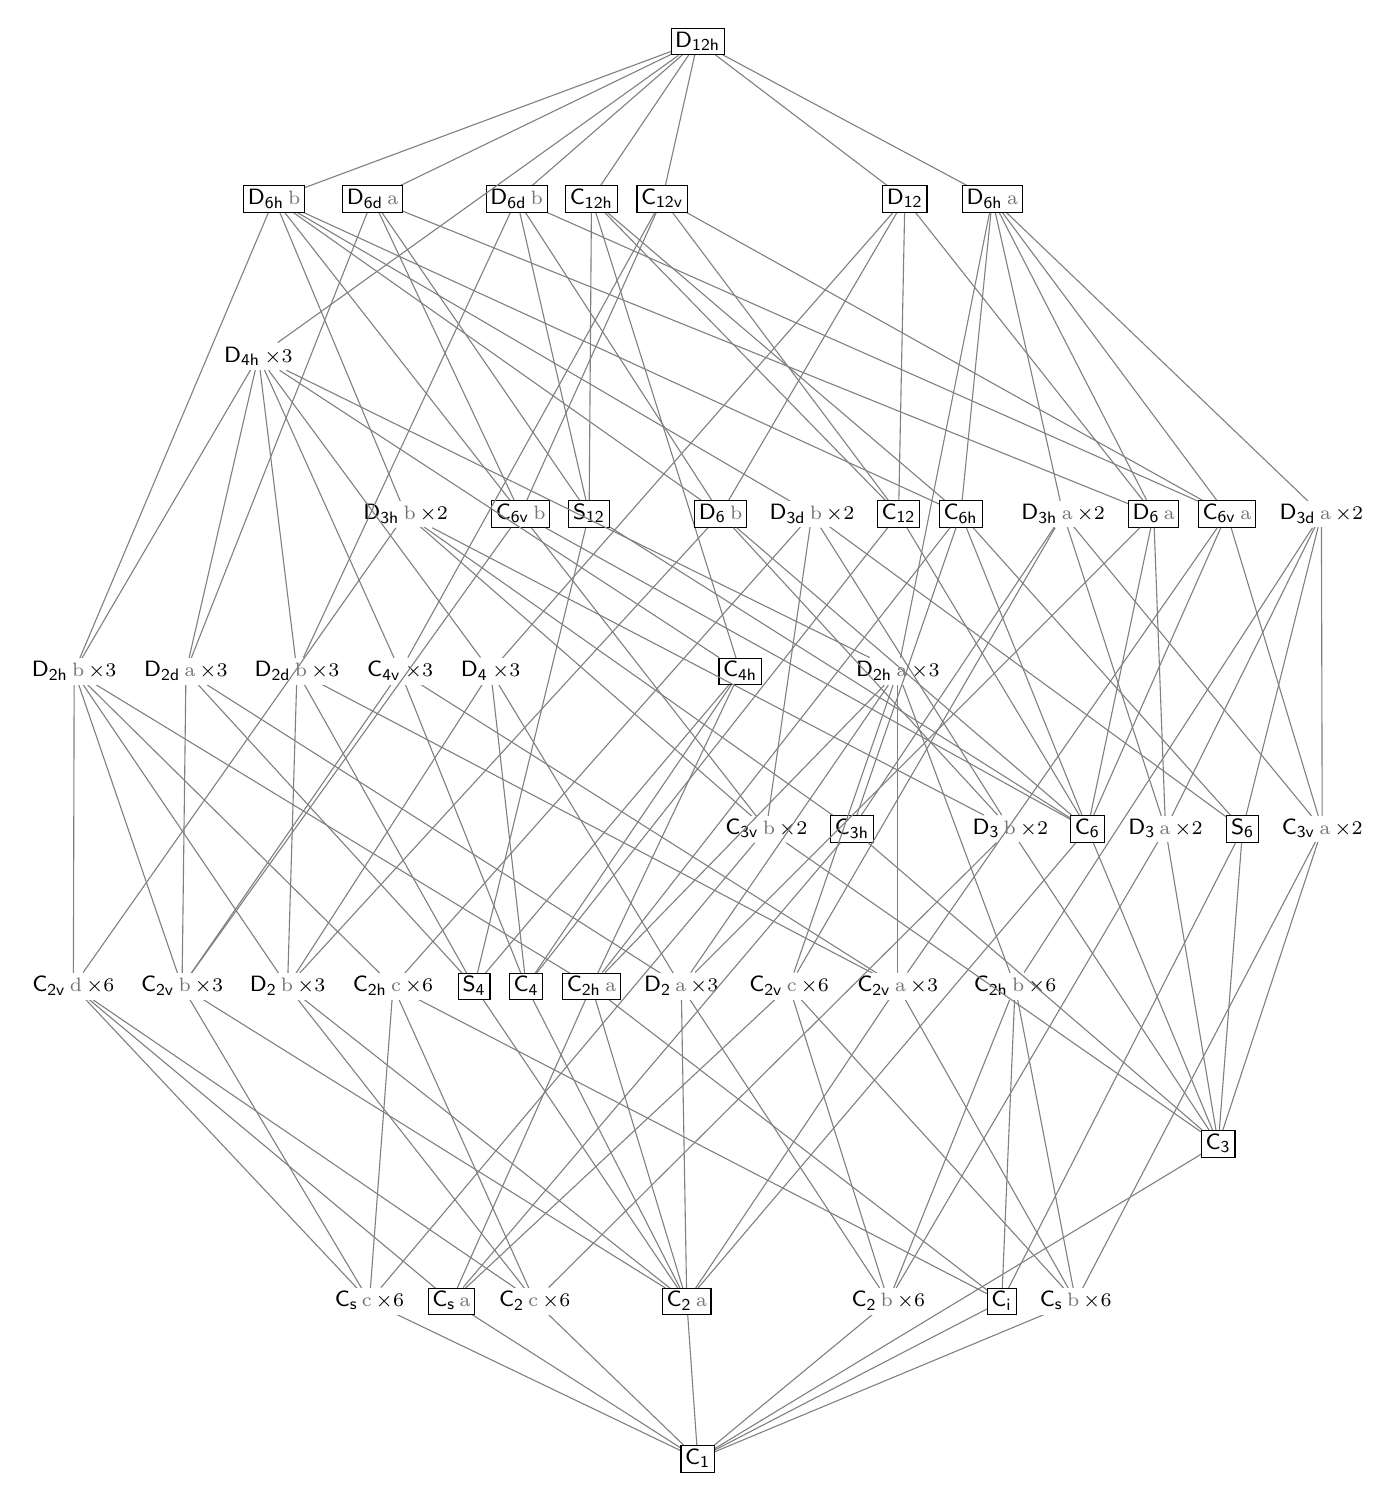
\begin{tikzpicture}[x=1cm, y=2.000cm,
  every node/.style={fill=white, font=\footnotesize, inner xsep=1.5pt, inner ysep=1.2pt, text height=5.6pt, text depth=1.6pt},
  normal/.style={draw, line width=0.4pt}, cover/.style={black!50, line width=0.4pt}]
\draw[cover] (0.00,0) -- (-0.14,1);
\draw[cover] (0.00,0) -- (2.42,1);
\draw[cover] (0.00,0) -- (-2.07,1);
\draw[cover] (0.00,0) -- (3.86,1);
\draw[cover] (0.00,0) -- (-3.13,1);
\draw[cover] (0.00,0) -- (4.80,1);
\draw[cover] (0.00,0) -- (-4.17,1);
\draw[cover] (0.00,0) -- (6.61,2);
\draw[cover] (-0.14,1) -- (-2.18,3);
\draw[cover] (-0.14,1) -- (-0.21,3);
\draw[cover] (-0.14,1) -- (-5.21,3);
\draw[cover] (-0.14,1) -- (-1.35,3);
\draw[cover] (-0.14,1) -- (-2.84,3);
\draw[cover] (-0.14,1) -- (2.54,3);
\draw[cover] (-0.14,1) -- (-6.55,3);
\draw[cover] (-0.14,1) -- (4.95,4);
\draw[cover] (2.42,1) -- (-0.21,3);
\draw[cover] (2.42,1) -- (4.03,3);
\draw[cover] (2.42,1) -- (1.16,3);
\draw[cover] (2.42,1) -- (5.94,4);
\draw[cover] (-2.07,1) -- (-5.21,3);
\draw[cover] (-2.07,1) -- (-3.87,3);
\draw[cover] (-2.07,1) -- (-7.93,3);
\draw[cover] (3.86,1) -- (-1.35,3);
\draw[cover] (3.86,1) -- (4.03,3);
\draw[cover] (3.86,1) -- (-3.87,3);
\draw[cover] (3.86,1) -- (6.92,4);
\draw[cover] (-3.13,1) -- (-1.35,3);
\draw[cover] (-3.13,1) -- (1.16,3);
\draw[cover] (-3.13,1) -- (-7.93,3);
\draw[cover] (4.80,1) -- (2.54,3);
\draw[cover] (4.80,1) -- (4.03,3);
\draw[cover] (4.80,1) -- (1.16,3);
\draw[cover] (4.80,1) -- (7.93,4);
\draw[cover] (-4.17,1) -- (-6.55,3);
\draw[cover] (-4.17,1) -- (-3.87,3);
\draw[cover] (-4.17,1) -- (-7.93,3);
\draw[cover] (6.61,2) -- (4.95,4);
\draw[cover] (6.61,2) -- (5.94,4);
\draw[cover] (6.61,2) -- (3.97,4);
\draw[cover] (6.61,2) -- (6.92,4);
\draw[cover] (6.61,2) -- (7.93,4);
\draw[cover] (-2.18,3) -- (-2.63,5);
\draw[cover] (-2.18,3) -- (0.54,5);
\draw[cover] (-2.18,3) -- (-3.78,5);
\draw[cover] (-2.18,3) -- (2.55,6);
\draw[cover] (-0.21,3) -- (-2.63,5);
\draw[cover] (-0.21,3) -- (-6.50,5);
\draw[cover] (-5.21,3) -- (-2.63,5);
\draw[cover] (-5.21,3) -- (-7.92,5);
\draw[cover] (-5.21,3) -- (-5.09,5);
\draw[cover] (-5.21,3) -- (0.29,6);
\draw[cover] (-1.35,3) -- (0.54,5);
\draw[cover] (-1.35,3) -- (-7.92,5);
\draw[cover] (-2.84,3) -- (0.54,5);
\draw[cover] (-2.84,3) -- (-6.50,5);
\draw[cover] (-2.84,3) -- (-5.09,5);
\draw[cover] (-2.84,3) -- (-1.38,6);
\draw[cover] (2.54,3) -- (-3.78,5);
\draw[cover] (2.54,3) -- (2.54,5);
\draw[cover] (2.54,3) -- (-5.09,5);
\draw[cover] (-6.55,3) -- (-3.78,5);
\draw[cover] (-6.55,3) -- (-6.50,5);
\draw[cover] (-6.55,3) -- (-7.92,5);
\draw[cover] (4.03,3) -- (2.54,5);
\draw[cover] (-3.87,3) -- (-7.92,5);
\draw[cover] (-3.87,3) -- (1.45,6);
\draw[cover] (-7.93,3) -- (-7.92,5);
\draw[cover] (4.95,4) -- (2.55,6);
\draw[cover] (4.95,4) -- (5.79,6);
\draw[cover] (4.95,4) -- (3.34,6);
\draw[cover] (4.95,4) -- (6.72,6);
\draw[cover] (4.95,4) -- (-2.25,6);
\draw[cover] (5.94,4) -- (5.79,6);
\draw[cover] (5.94,4) -- (7.92,6);
\draw[cover] (5.94,4) -- (4.64,6);
\draw[cover] (6.92,4) -- (3.34,6);
\draw[cover] (6.92,4) -- (7.92,6);
\draw[cover] (6.92,4) -- (1.45,6);
\draw[cover] (1.96,4) -- (4.64,6);
\draw[cover] (1.96,4) -- (-3.71,6);
\draw[cover] (7.93,4) -- (6.72,6);
\draw[cover] (7.93,4) -- (7.92,6);
\draw[cover] (7.93,4) -- (4.64,6);
\draw[cover] (0.87,4) -- (-2.25,6);
\draw[cover] (0.87,4) -- (1.45,6);
\draw[cover] (0.87,4) -- (-3.71,6);
\draw[cover] (-2.63,5) -- (2.63,8);
\draw[cover] (0.54,5) -- (-1.35,8);
\draw[cover] (-3.78,5) -- (-5.58,7);
\draw[cover] (2.54,5) -- (3.74,8);
\draw[cover] (-6.50,5) -- (-5.58,7);
\draw[cover] (-6.50,5) -- (-4.13,8);
\draw[cover] (-7.92,5) -- (-5.58,7);
\draw[cover] (-7.92,5) -- (-5.38,8);
\draw[cover] (-5.09,5) -- (-5.58,7);
\draw[cover] (2.55,6) -- (2.63,8);
\draw[cover] (2.55,6) -- (-1.35,8);
\draw[cover] (2.55,6) -- (-0.45,8);
\draw[cover] (5.79,6) -- (2.63,8);
\draw[cover] (5.79,6) -- (3.74,8);
\draw[cover] (5.79,6) -- (-4.13,8);
\draw[cover] (0.29,6) -- (2.63,8);
\draw[cover] (0.29,6) -- (-5.38,8);
\draw[cover] (0.29,6) -- (-2.30,8);
\draw[cover] (3.34,6) -- (-1.35,8);
\draw[cover] (3.34,6) -- (3.74,8);
\draw[cover] (3.34,6) -- (-5.38,8);
\draw[cover] (-1.38,6) -- (-1.35,8);
\draw[cover] (-1.38,6) -- (-4.13,8);
\draw[cover] (-1.38,6) -- (-2.30,8);
\draw[cover] (6.72,6) -- (-0.45,8);
\draw[cover] (6.72,6) -- (3.74,8);
\draw[cover] (6.72,6) -- (-2.30,8);
\draw[cover] (-2.25,6) -- (-0.45,8);
\draw[cover] (-2.25,6) -- (-4.13,8);
\draw[cover] (-2.25,6) -- (-5.38,8);
\draw[cover] (7.92,6) -- (3.74,8);
\draw[cover] (4.64,6) -- (3.74,8);
\draw[cover] (1.45,6) -- (-5.38,8);
\draw[cover] (-3.71,6) -- (-5.38,8);
\draw[cover] (2.63,8) -- (0.00,9);
\draw[cover] (-1.35,8) -- (0.00,9);
\draw[cover] (-0.45,8) -- (0.00,9);
\draw[cover] (3.74,8) -- (0.00,9);
\draw[cover] (-4.13,8) -- (0.00,9);
\draw[cover] (-5.38,8) -- (0.00,9);
\draw[cover] (-2.30,8) -- (0.00,9);
\node[normal] (n00) at (0.00,0) {$\grp{C_{1}}$};
\node[normal] (n01) at (-0.14,1) {$\grp{C_{2}}$\clsletter{a}};
\node (n02) at (2.42,1) {$\grp{C_{2}}$\clsletter{b}\,\nconj{6}};
\node (n03) at (-2.07,1) {$\grp{C_{2}}$\clsletter{c}\,\nconj{6}};
\node[normal] (n04) at (3.86,1) {$\grp{C_{i}}$};
\node[normal] (n05) at (-3.13,1) {$\grp{C_{s}}$\clsletter{a}};
\node (n06) at (4.80,1) {$\grp{C_{s}}$\clsletter{b}\,\nconj{6}};
\node (n07) at (-4.17,1) {$\grp{C_{s}}$\clsletter{c}\,\nconj{6}};
\node[normal] (n08) at (6.61,2) {$\grp{C_{3}}$};
\node[normal] (n09) at (-2.18,3) {$\grp{C_{4}}$};
\node (n10) at (-0.21,3) {$\grp{D_{2}}$\clsletter{a}\,\nconj{3}};
\node (n11) at (-5.21,3) {$\grp{D_{2}}$\clsletter{b}\,\nconj{3}};
\node[normal] (n12) at (-1.35,3) {$\grp{C_{2h}}$\clsletter{a}};
\node[normal] (n13) at (-2.84,3) {$\grp{S_{4}}$};
\node (n14) at (2.54,3) {$\grp{C_{2v}}$\clsletter{a}\,\nconj{3}};
\node (n15) at (-6.55,3) {$\grp{C_{2v}}$\clsletter{b}\,\nconj{3}};
\node (n16) at (4.03,3) {$\grp{C_{2h}}$\clsletter{b}\,\nconj{6}};
\node (n17) at (1.16,3) {$\grp{C_{2v}}$\clsletter{c}\,\nconj{6}};
\node (n18) at (-3.87,3) {$\grp{C_{2h}}$\clsletter{c}\,\nconj{6}};
\node (n19) at (-7.93,3) {$\grp{C_{2v}}$\clsletter{d}\,\nconj{6}};
\node[normal] (n20) at (4.95,4) {$\grp{C_{6}}$};
\node (n21) at (5.94,4) {$\grp{D_{3}}$\clsletter{a}\,\nconj{2}};
\node (n22) at (3.97,4) {$\grp{D_{3}}$\clsletter{b}\,\nconj{2}};
\node[normal] (n23) at (6.92,4) {$\grp{S_{6}}$};
\node[normal] (n24) at (1.96,4) {$\grp{C_{3h}}$};
\node (n25) at (7.93,4) {$\grp{C_{3v}}$\clsletter{a}\,\nconj{2}};
\node (n26) at (0.87,4) {$\grp{C_{3v}}$\clsletter{b}\,\nconj{2}};
\node (n27) at (-2.63,5) {$\grp{D_{4}}$\,\nconj{3}};
\node[normal] (n28) at (0.54,5) {$\grp{C_{4h}}$};
\node (n29) at (-3.78,5) {$\grp{C_{4v}}$\,\nconj{3}};
\node (n30) at (2.54,5) {$\grp{D_{2h}}$\clsletter{a}\,\nconj{3}};
\node (n31) at (-6.50,5) {$\grp{D_{2d}}$\clsletter{a}\,\nconj{3}};
\node (n32) at (-7.92,5) {$\grp{D_{2h}}$\clsletter{b}\,\nconj{3}};
\node (n33) at (-5.09,5) {$\grp{D_{2d}}$\clsletter{b}\,\nconj{3}};
\node[normal] (n34) at (2.55,6) {$\grp{C_{12}}$};
\node[normal] (n35) at (5.79,6) {$\grp{D_{6}}$\clsletter{a}};
\node[normal] (n36) at (0.29,6) {$\grp{D_{6}}$\clsletter{b}};
\node[normal] (n37) at (3.34,6) {$\grp{C_{6h}}$};
\node[normal] (n38) at (-1.38,6) {$\grp{S_{12}}$};
\node[normal] (n39) at (6.72,6) {$\grp{C_{6v}}$\clsletter{a}};
\node[normal] (n40) at (-2.25,6) {$\grp{C_{6v}}$\clsletter{b}};
\node (n41) at (7.92,6) {$\grp{D_{3d}}$\clsletter{a}\,\nconj{2}};
\node (n42) at (4.64,6) {$\grp{D_{3h}}$\clsletter{a}\,\nconj{2}};
\node (n43) at (1.45,6) {$\grp{D_{3d}}$\clsletter{b}\,\nconj{2}};
\node (n44) at (-3.71,6) {$\grp{D_{3h}}$\clsletter{b}\,\nconj{2}};
\node (n45) at (-5.58,7) {$\grp{D_{4h}}$\,\nconj{3}};
\node[normal] (n46) at (2.63,8) {$\grp{D_{12}}$};
\node[normal] (n47) at (-1.35,8) {$\grp{C_{12h}}$};
\node[normal] (n48) at (-0.45,8) {$\grp{C_{12v}}$};
\node[normal] (n49) at (3.74,8) {$\grp{D_{6h}}$\clsletter{a}};
\node[normal] (n50) at (-4.13,8) {$\grp{D_{6d}}$\clsletter{a}};
\node[normal] (n51) at (-5.38,8) {$\grp{D_{6h}}$\clsletter{b}};
\node[normal] (n52) at (-2.30,8) {$\grp{D_{6d}}$\clsletter{b}};
\node[normal] (n53) at (0.00,9) {$\grp{D_{12h}}$};
\draw[cover] (n03) -- (n22);
\draw[cover] (n05) -- (n24);
\draw[cover] (n07) -- (n26);
\draw[cover] (n08) -- (n24);
\draw[cover] (n08) -- (n26);
\draw[cover] (n10) -- (n30);
\draw[cover] (n10) -- (n35);
\draw[cover] (n12) -- (n30);
\draw[cover] (n12) -- (n37);
\draw[cover] (n14) -- (n39);
\draw[cover] (n15) -- (n40);
\draw[cover] (n16) -- (n41);
\draw[cover] (n17) -- (n30);
\draw[cover] (n17) -- (n42);
\draw[cover] (n19) -- (n44);
\draw[cover] (n20) -- (n36);
\draw[cover] (n20) -- (n38);
\draw[cover] (n22) -- (n36);
\draw[cover] (n22) -- (n43);
\draw[cover] (n22) -- (n44);
\draw[cover] (n24) -- (n37);
\draw[cover] (n27) -- (n45);
\draw[cover] (n28) -- (n45);
\draw[cover] (n29) -- (n48);
\draw[cover] (n30) -- (n45);
\draw[cover] (n33) -- (n52);
\draw[cover] (n45) -- (n53);
\end{tikzpicture}
\end{center}
{\small\setlength{\fillwidth}{\textwidth}\addtolength{\fillwidth}{-12\tabcolsep}\setlength{\colwidth}{0pt}\cellmax{$\grp{C_{s}}$\clsletter{a} $\samecls$ $\grp{C_{1v}}$ $\samecls$ $\grp{C_{1h}}$}\cellmax{$\grp{C_{s}}$\clsletter{b} $\samecls$ $\grp{C_{1v}}$ $\samecls$ $\grp{C_{1h}}$}\cellmax{$\grp{C_{s}}$\clsletter{c} $\samecls$ $\grp{C_{1v}}$ $\samecls$ $\grp{C_{1h}}$}\cellmax{$\grp{C_{2h}}$\clsletter{a} $\samecls$ $\grp{D_{1d}}$}\cellmax{$\grp{C_{2h}}$\clsletter{b} $\samecls$ $\grp{D_{1d}}$}\cellmax{$\grp{C_{2h}}$\clsletter{c} $\samecls$ $\grp{D_{1d}}$}\cellmax{$\grp{C_{2v}}$\clsletter{a} $\samecls$ $\grp{D_{1h}}$}\cellmax{$\grp{C_{2v}}$\clsletter{b} $\samecls$ $\grp{D_{1h}}$}\cellmax{$\grp{C_{2v}}$\clsletter{c} $\samecls$ $\grp{D_{1h}}$}\cellmax{$\grp{C_{2v}}$\clsletter{d} $\samecls$ $\grp{D_{1h}}$}\cellmax{$\grp{C_{2}}$\clsletter{a} $\samecls$ $\grp{D_{1}}$}\cellmax{$\grp{C_{2}}$\clsletter{b} $\samecls$ $\grp{D_{1}}$}\cellmax{$\grp{C_{2}}$\clsletter{c} $\samecls$ $\grp{D_{1}}$}\cellmax{$\grp{C_{i}}$ $\samecls$ $\grp{S_{2}}$}\cellmax{subgrp}\cellmax{$\grp{C_{12h}}$}\addtolength{\fillwidth}{-\colwidth}\setlength{\colwidth}{0pt}\cellmax{order}\cellmax{12}\cellmax{16}\cellmax{24}\cellmax{48}\cellmax{1}\cellmax{2}\cellmax{3}\cellmax{4}\cellmax{6}\cellmax{8}\addtolength{\fillwidth}{-\colwidth}\setlength{\colwidth}{0pt}\cellmax{conjugates}\cellmax{1}\cellmax{2}\cellmax{3}\cellmax{6}\addtolength{\fillwidth}{-\colwidth}\setlength{\colwidth}{0pt}\cellmax{normal}\cellmax{yes}\cellmax{no}\addtolength{\fillwidth}{-\colwidth}\setlength{\colwidth}{0pt}\cellmax{$\grp{N}_{\hairsp \grp{D_{12h}}}(\grp{H})$}\cellmax{$\grp{D_{12h}}$}\cellmax{$\grp{D_{2h}}$\clsletter{a}}\cellmax{$\grp{D_{2h}}$\clsletter{b}}\cellmax{$\grp{D_{6h}}$\clsletter{a}}\cellmax{$\grp{D_{6h}}$\clsletter{b}}\cellmax{$\grp{D_{4h}}$}\addtolength{\fillwidth}{-\colwidth}\setlength{\colwidth}{0pt}\cellmax{$\grp{C}_{\hairsp \grp{D_{12h}}}(\grp{H})$}\cellmax{$\grp{C_{12h}}$}\cellmax{$\grp{C_{2h}}$\clsletter{a}}\cellmax{$\grp{D_{12h}}$}\cellmax{$\grp{D_{2h}}$\clsletter{a}}\cellmax{$\grp{D_{2h}}$\clsletter{b}}\addtolength{\fillwidth}{-\colwidth}\setlength{\colwidth}{0pt}\cellmax{$\cls{2C_{12}}$, $\cls{2C_{6}}$, $\cls{2C_{4}}$, $\cls{2C_{3}}$, $\cls{2C_{12}^{5}}$, $\cls{C_{2}}$, $\cls{i}$, $\cls{\sigma_{h}}$, $\cls{2S_{12}}$, $\cls{2S_{6}}$, $\cls{2S_{4}}$, $\cls{2S_{3}}$, $\cls{2S_{12}^{5}}$}\cellmax{$\cls{2C_{12}}$, $\cls{2C_{6}}$, $\cls{2C_{4}}$, $\cls{2C_{3}}$, $\cls{2C_{12}^{5}}$, $\cls{C_{2}}$, $\cls{6C_{2}'}$, $\cls{6C_{2}''}$}\cellmax{$\cls{2C_{6}}$, $\cls{2C_{3}}$, $\cls{C_{2}}$, $\cls{6C_{2}''}$, $\cls{2S_{12}}$, $\cls{2S_{4}}$, $\cls{2S_{12}^{5}}$, $\cls{6\sigma_{v}}$}\cellmax{$\cls{2C_{4}}$, $\cls{C_{2}}$, $\cls{6C_{2}'}$, $\cls{6C_{2}''}$, $\cls{i}$, $\cls{\sigma_{h}}$, $\cls{2S_{4}}$, $\cls{6\sigma_{v}}$, $\cls{6\sigma_{d}}$}\cellmax{$\cls{2C_{6}}$, $\cls{2C_{3}}$, $\cls{C_{2}}$, $\cls{6C_{2}'}$, $\cls{2S_{12}}$, $\cls{2S_{4}}$, $\cls{2S_{12}^{5}}$, $\cls{6\sigma_{d}}$}\cellmax{$\cls{2C_{12}}$, $\cls{2C_{6}}$, $\cls{2C_{4}}$, $\cls{2C_{3}}$, $\cls{2C_{12}^{5}}$, $\cls{C_{2}}$, $\cls{6\sigma_{v}}$, $\cls{6\sigma_{d}}$}\cellmax{$\cls{2C_{6}}$, $\cls{2C_{3}}$, $\cls{C_{2}}$, $\cls{6C_{2}''}$, $\cls{i}$, $\cls{\sigma_{h}}$, $\cls{2S_{6}}$, $\cls{2S_{3}}$, $\cls{6\sigma_{d}}$}\cellmax{$\cls{2C_{6}}$, $\cls{2C_{3}}$, $\cls{C_{2}}$, $\cls{6C_{2}'}$, $\cls{i}$, $\cls{\sigma_{h}}$, $\cls{2S_{6}}$, $\cls{2S_{3}}$, $\cls{6\sigma_{v}}$}\cellmax{$\cls{2C_{12}}$, $\cls{2C_{6}}$, $\cls{2C_{4}}$, $\cls{2C_{3}}$, $\cls{2C_{12}^{5}}$, $\cls{C_{2}}$}\cellmax{$\cls{2C_{6}}$, $\cls{2C_{3}}$, $\cls{C_{2}}$, $\cls{2S_{12}}$, $\cls{2S_{4}}$, $\cls{2S_{12}^{5}}$}\cellmax{$\cls{2C_{6}}$, $\cls{2C_{3}}$, $\cls{C_{2}}$, $\cls{i}$, $\cls{\sigma_{h}}$, $\cls{2S_{6}}$, $\cls{2S_{3}}$}\cellmax{$\cls{2C_{3}}$, $\cls{6C_{2}''}$, $\cls{\sigma_{h}}$, $\cls{2S_{3}}$, $\cls{6\sigma_{d}}$}\cellmax{$\cls{2C_{3}}$, $\cls{6C_{2}''}$, $\cls{i}$, $\cls{2S_{6}}$, $\cls{6\sigma_{d}}$}\cellmax{$\cls{2C_{3}}$, $\cls{6C_{2}'}$, $\cls{\sigma_{h}}$, $\cls{2S_{3}}$, $\cls{6\sigma_{v}}$}\cellmax{$\cls{2C_{3}}$, $\cls{6C_{2}'}$, $\cls{i}$, $\cls{2S_{6}}$, $\cls{6\sigma_{v}}$}\cellmax{$\cls{2C_{4}}$, $\cls{C_{2}}$, $\cls{6C_{2}'}$, $\cls{6C_{2}''}$}\cellmax{$\cls{C_{2}}$, $\cls{6C_{2}''}$, $\cls{i}$, $\cls{\sigma_{h}}$, $\cls{6\sigma_{d}}$}\cellmax{$\cls{2C_{6}}$, $\cls{2C_{3}}$, $\cls{C_{2}}$, $\cls{6C_{2}''}$}\cellmax{$\cls{C_{2}}$, $\cls{6C_{2}''}$, $\cls{2S_{4}}$, $\cls{6\sigma_{v}}$}\cellmax{$\cls{C_{2}}$, $\cls{6C_{2}'}$, $\cls{i}$, $\cls{\sigma_{h}}$, $\cls{6\sigma_{v}}$}\cellmax{$\cls{2C_{4}}$, $\cls{C_{2}}$, $\cls{i}$, $\cls{\sigma_{h}}$, $\cls{2S_{4}}$}\cellmax{$\cls{2C_{6}}$, $\cls{2C_{3}}$, $\cls{C_{2}}$, $\cls{6C_{2}'}$}\cellmax{$\cls{C_{2}}$, $\cls{6C_{2}'}$, $\cls{2S_{4}}$, $\cls{6\sigma_{d}}$}\cellmax{$\cls{2C_{4}}$, $\cls{C_{2}}$, $\cls{6\sigma_{v}}$, $\cls{6\sigma_{d}}$}\cellmax{$\cls{2C_{6}}$, $\cls{2C_{3}}$, $\cls{C_{2}}$, $\cls{6\sigma_{d}}$}\cellmax{$\cls{2C_{6}}$, $\cls{2C_{3}}$, $\cls{C_{2}}$, $\cls{6\sigma_{v}}$}\cellmax{$\cls{6C_{2}''}$, $\cls{\sigma_{h}}$, $\cls{6\sigma_{d}}$}\cellmax{$\cls{6C_{2}''}$, $\cls{i}$, $\cls{6\sigma_{d}}$}\cellmax{$\cls{6C_{2}'}$, $\cls{\sigma_{h}}$, $\cls{6\sigma_{v}}$}\cellmax{$\cls{2C_{3}}$, $\cls{\sigma_{h}}$, $\cls{2S_{3}}$}\cellmax{$\cls{2C_{6}}$, $\cls{2C_{3}}$, $\cls{C_{2}}$}\cellmax{$\cls{6C_{2}'}$, $\cls{i}$, $\cls{6\sigma_{v}}$}\cellmax{$\cls{2C_{3}}$, $\cls{6C_{2}''}$}\cellmax{$\cls{2C_{3}}$, $\cls{i}$, $\cls{2S_{6}}$}\cellmax{$\cls{2C_{3}}$, $\cls{6C_{2}'}$}\cellmax{$\cls{C_{2}}$, $\cls{6C_{2}''}$}\cellmax{$\cls{2C_{3}}$, $\cls{6\sigma_{d}}$}\cellmax{$\cls{2C_{3}}$, $\cls{6\sigma_{v}}$}\cellmax{$\cls{C_{2}}$, $\cls{6C_{2}'}$}\cellmax{$\cls{C_{2}}$, $\cls{i}$, $\cls{\sigma_{h}}$}\cellmax{classes}\cellmax{$\cls{2C_{4}}$, $\cls{C_{2}}$}\cellmax{$\cls{C_{2}}$, $\cls{2S_{4}}$}\cellmax{$\cls{C_{2}}$, $\cls{6\sigma_{d}}$}\cellmax{$\cls{C_{2}}$, $\cls{6\sigma_{v}}$}\cellmax{$\cls{6C_{2}''}$}\cellmax{$\cls{6C_{2}'}$}\cellmax{$\cls{2C_{3}}$}\cellmax{$\cls{6\sigma_{d}}$}\cellmax{$\cls{6\sigma_{v}}$}\cellmax{---}\cellmax{all}\cellmax{$\cls{C_{2}}$}\cellmax{$\cls{\sigma_{h}}$}\cellmax{$\cls{i}$}\fillcap\begin{longtable}{@{}lrrlll>{\RaggedRight\arraybackslash}p{\fillwidth}@{}}\toprule
subgrp & order & conjugates & normal & $\grp{N}_{\hairsp \grp{D_{12h}}}(\grp{H})$ & $\grp{C}_{\hairsp \grp{D_{12h}}}(\grp{H})$ & classes\\\midrule\endhead
\bottomrule\endfoot\endlastfoot
\href{C1.pdf}{$\grp{C_{1}}$} & 1 & 1 & yes & \href{D12h.pdf}{$\grp{D_{12h}}$} & \href{D12h.pdf}{$\grp{D_{12h}}$} & ---\\*
\href{C2.pdf}{$\grp{C_{2}}$}\clsletter{a} $\samecls$ \href{D1.pdf}{$\grp{D_{1}}$} & 2 & 1 & yes & \href{D12h.pdf}{$\grp{D_{12h}}$} & \href{D12h.pdf}{$\grp{D_{12h}}$} & $\cls{C_{2}}$\\
\href{C2.pdf}{$\grp{C_{2}}$}\clsletter{b} $\samecls$ \href{D1.pdf}{$\grp{D_{1}}$} & 2 & 6 & no & \href{D2h.pdf}{$\grp{D_{2h}}$}\clsletter{a} & \href{D2h.pdf}{$\grp{D_{2h}}$}\clsletter{a} & $\cls{6C_{2}'}$\\
\href{C2.pdf}{$\grp{C_{2}}$}\clsletter{c} $\samecls$ \href{D1.pdf}{$\grp{D_{1}}$} & 2 & 6 & no & \href{D2h.pdf}{$\grp{D_{2h}}$}\clsletter{b} & \href{D2h.pdf}{$\grp{D_{2h}}$}\clsletter{b} & $\cls{6C_{2}''}$\\
\href{S2.pdf}{$\grp{C_{i}}$} $\samecls$ \href{S2.pdf}{$\grp{S_{2}}$} & 2 & 1 & yes & \href{D12h.pdf}{$\grp{D_{12h}}$} & \href{D12h.pdf}{$\grp{D_{12h}}$} & $\cls{i}$\\
\href{C1v.pdf}{$\grp{C_{s}}$}\clsletter{a} $\samecls$ \href{C1v.pdf}{$\grp{C_{1v}}$} $\samecls$ \href{C1h.pdf}{$\grp{C_{1h}}$} & 2 & 1 & yes & \href{D12h.pdf}{$\grp{D_{12h}}$} & \href{D12h.pdf}{$\grp{D_{12h}}$} & $\cls{\sigma_{h}}$\\
\href{C1v.pdf}{$\grp{C_{s}}$}\clsletter{b} $\samecls$ \href{C1v.pdf}{$\grp{C_{1v}}$} $\samecls$ \href{C1h.pdf}{$\grp{C_{1h}}$} & 2 & 6 & no & \href{D2h.pdf}{$\grp{D_{2h}}$}\clsletter{a} & \href{D2h.pdf}{$\grp{D_{2h}}$}\clsletter{a} & $\cls{6\sigma_{v}}$\\
\href{C1v.pdf}{$\grp{C_{s}}$}\clsletter{c} $\samecls$ \href{C1v.pdf}{$\grp{C_{1v}}$} $\samecls$ \href{C1h.pdf}{$\grp{C_{1h}}$} & 2 & 6 & no & \href{D2h.pdf}{$\grp{D_{2h}}$}\clsletter{b} & \href{D2h.pdf}{$\grp{D_{2h}}$}\clsletter{b} & $\cls{6\sigma_{d}}$\\
\href{C3.pdf}{$\grp{C_{3}}$} & 3 & 1 & yes & \href{D12h.pdf}{$\grp{D_{12h}}$} & \href{C12h.pdf}{$\grp{C_{12h}}$} & $\cls{2C_{3}}$\\
\href{C4.pdf}{$\grp{C_{4}}$} & 4 & 1 & yes & \href{D12h.pdf}{$\grp{D_{12h}}$} & \href{C12h.pdf}{$\grp{C_{12h}}$} & $\cls{2C_{4}}$, $\cls{C_{2}}$\\
\href{S4.pdf}{$\grp{S_{4}}$} & 4 & 1 & yes & \href{D12h.pdf}{$\grp{D_{12h}}$} & \href{C12h.pdf}{$\grp{C_{12h}}$} & $\cls{C_{2}}$, $\cls{2S_{4}}$\\
\href{C2h.pdf}{$\grp{C_{2h}}$}\clsletter{a} $\samecls$ \href{D1d.pdf}{$\grp{D_{1d}}$} & 4 & 1 & yes & \href{D12h.pdf}{$\grp{D_{12h}}$} & \href{D12h.pdf}{$\grp{D_{12h}}$} & $\cls{C_{2}}$, $\cls{i}$, $\cls{\sigma_{h}}$\\
\href{C2h.pdf}{$\grp{C_{2h}}$}\clsletter{b} $\samecls$ \href{D1d.pdf}{$\grp{D_{1d}}$} & 4 & 6 & no & \href{D2h.pdf}{$\grp{D_{2h}}$}\clsletter{a} & \href{D2h.pdf}{$\grp{D_{2h}}$}\clsletter{a} & $\cls{6C_{2}'}$, $\cls{i}$, $\cls{6\sigma_{v}}$\\
\href{C2h.pdf}{$\grp{C_{2h}}$}\clsletter{c} $\samecls$ \href{D1d.pdf}{$\grp{D_{1d}}$} & 4 & 6 & no & \href{D2h.pdf}{$\grp{D_{2h}}$}\clsletter{b} & \href{D2h.pdf}{$\grp{D_{2h}}$}\clsletter{b} & $\cls{6C_{2}''}$, $\cls{i}$, $\cls{6\sigma_{d}}$\\
\href{C2v.pdf}{$\grp{C_{2v}}$}\clsletter{a} $\samecls$ \href{D1h.pdf}{$\grp{D_{1h}}$} & 4 & 3 & no & \href{D4h.pdf}{$\grp{D_{4h}}$} & \href{D2h.pdf}{$\grp{D_{2h}}$}\clsletter{a} & $\cls{C_{2}}$, $\cls{6\sigma_{v}}$\\
\href{C2v.pdf}{$\grp{C_{2v}}$}\clsletter{b} $\samecls$ \href{D1h.pdf}{$\grp{D_{1h}}$} & 4 & 3 & no & \href{D4h.pdf}{$\grp{D_{4h}}$} & \href{D2h.pdf}{$\grp{D_{2h}}$}\clsletter{b} & $\cls{C_{2}}$, $\cls{6\sigma_{d}}$\\
\href{C2v.pdf}{$\grp{C_{2v}}$}\clsletter{c} $\samecls$ \href{D1h.pdf}{$\grp{D_{1h}}$} & 4 & 6 & no & \href{D2h.pdf}{$\grp{D_{2h}}$}\clsletter{a} & \href{D2h.pdf}{$\grp{D_{2h}}$}\clsletter{a} & $\cls{6C_{2}'}$, $\cls{\sigma_{h}}$, $\cls{6\sigma_{v}}$\\
\href{C2v.pdf}{$\grp{C_{2v}}$}\clsletter{d} $\samecls$ \href{D1h.pdf}{$\grp{D_{1h}}$} & 4 & 6 & no & \href{D2h.pdf}{$\grp{D_{2h}}$}\clsletter{b} & \href{D2h.pdf}{$\grp{D_{2h}}$}\clsletter{b} & $\cls{6C_{2}''}$, $\cls{\sigma_{h}}$, $\cls{6\sigma_{d}}$\\
\href{D2.pdf}{$\grp{D_{2}}$}\clsletter{a} & 4 & 3 & no & \href{D4h.pdf}{$\grp{D_{4h}}$} & \href{D2h.pdf}{$\grp{D_{2h}}$}\clsletter{a} & $\cls{C_{2}}$, $\cls{6C_{2}'}$\\
\href{D2.pdf}{$\grp{D_{2}}$}\clsletter{b} & 4 & 3 & no & \href{D4h.pdf}{$\grp{D_{4h}}$} & \href{D2h.pdf}{$\grp{D_{2h}}$}\clsletter{b} & $\cls{C_{2}}$, $\cls{6C_{2}''}$\\
\href{C6.pdf}{$\grp{C_{6}}$} & 6 & 1 & yes & \href{D12h.pdf}{$\grp{D_{12h}}$} & \href{C12h.pdf}{$\grp{C_{12h}}$} & $\cls{2C_{6}}$, $\cls{2C_{3}}$, $\cls{C_{2}}$\\
\href{S6.pdf}{$\grp{S_{6}}$} & 6 & 1 & yes & \href{D12h.pdf}{$\grp{D_{12h}}$} & \href{C12h.pdf}{$\grp{C_{12h}}$} & $\cls{2C_{3}}$, $\cls{i}$, $\cls{2S_{6}}$\\
\href{C3h.pdf}{$\grp{C_{3h}}$} & 6 & 1 & yes & \href{D12h.pdf}{$\grp{D_{12h}}$} & \href{C12h.pdf}{$\grp{C_{12h}}$} & $\cls{2C_{3}}$, $\cls{\sigma_{h}}$, $\cls{2S_{3}}$\\
\href{C3v.pdf}{$\grp{C_{3v}}$}\clsletter{a} & 6 & 2 & no & \href{D6h.pdf}{$\grp{D_{6h}}$}\clsletter{a} & \href{C2h.pdf}{$\grp{C_{2h}}$}\clsletter{a} & $\cls{2C_{3}}$, $\cls{6\sigma_{v}}$\\
\href{C3v.pdf}{$\grp{C_{3v}}$}\clsletter{b} & 6 & 2 & no & \href{D6h.pdf}{$\grp{D_{6h}}$}\clsletter{b} & \href{C2h.pdf}{$\grp{C_{2h}}$}\clsletter{a} & $\cls{2C_{3}}$, $\cls{6\sigma_{d}}$\\
\href{D3.pdf}{$\grp{D_{3}}$}\clsletter{a} & 6 & 2 & no & \href{D6h.pdf}{$\grp{D_{6h}}$}\clsletter{a} & \href{C2h.pdf}{$\grp{C_{2h}}$}\clsletter{a} & $\cls{2C_{3}}$, $\cls{6C_{2}'}$\\
\href{D3.pdf}{$\grp{D_{3}}$}\clsletter{b} & 6 & 2 & no & \href{D6h.pdf}{$\grp{D_{6h}}$}\clsletter{b} & \href{C2h.pdf}{$\grp{C_{2h}}$}\clsletter{a} & $\cls{2C_{3}}$, $\cls{6C_{2}''}$\\
\href{C4h.pdf}{$\grp{C_{4h}}$} & 8 & 1 & yes & \href{D12h.pdf}{$\grp{D_{12h}}$} & \href{C12h.pdf}{$\grp{C_{12h}}$} & $\cls{2C_{4}}$, $\cls{C_{2}}$, $\cls{i}$, $\cls{\sigma_{h}}$, $\cls{2S_{4}}$\\
\href{C4v.pdf}{$\grp{C_{4v}}$} & 8 & 3 & no & \href{D4h.pdf}{$\grp{D_{4h}}$} & \href{C2h.pdf}{$\grp{C_{2h}}$}\clsletter{a} & $\cls{2C_{4}}$, $\cls{C_{2}}$, $\cls{6\sigma_{v}}$, $\cls{6\sigma_{d}}$\\
\href{D4.pdf}{$\grp{D_{4}}$} & 8 & 3 & no & \href{D4h.pdf}{$\grp{D_{4h}}$} & \href{C2h.pdf}{$\grp{C_{2h}}$}\clsletter{a} & $\cls{2C_{4}}$, $\cls{C_{2}}$, $\cls{6C_{2}'}$, $\cls{6C_{2}''}$\\
\href{D2h.pdf}{$\grp{D_{2h}}$}\clsletter{a} & 8 & 3 & no & \href{D4h.pdf}{$\grp{D_{4h}}$} & \href{D2h.pdf}{$\grp{D_{2h}}$}\clsletter{a} & $\cls{C_{2}}$, $\cls{6C_{2}'}$, $\cls{i}$, $\cls{\sigma_{h}}$, $\cls{6\sigma_{v}}$\\
\href{D2h.pdf}{$\grp{D_{2h}}$}\clsletter{b} & 8 & 3 & no & \href{D4h.pdf}{$\grp{D_{4h}}$} & \href{D2h.pdf}{$\grp{D_{2h}}$}\clsletter{b} & $\cls{C_{2}}$, $\cls{6C_{2}''}$, $\cls{i}$, $\cls{\sigma_{h}}$, $\cls{6\sigma_{d}}$\\
\href{D2d.pdf}{$\grp{D_{2d}}$}\clsletter{a} & 8 & 3 & no & \href{D4h.pdf}{$\grp{D_{4h}}$} & \href{C2h.pdf}{$\grp{C_{2h}}$}\clsletter{a} & $\cls{C_{2}}$, $\cls{6C_{2}'}$, $\cls{2S_{4}}$, $\cls{6\sigma_{d}}$\\
\href{D2d.pdf}{$\grp{D_{2d}}$}\clsletter{b} & 8 & 3 & no & \href{D4h.pdf}{$\grp{D_{4h}}$} & \href{C2h.pdf}{$\grp{C_{2h}}$}\clsletter{a} & $\cls{C_{2}}$, $\cls{6C_{2}''}$, $\cls{2S_{4}}$, $\cls{6\sigma_{v}}$\\
\href{C12.pdf}{$\grp{C_{12}}$} & 12 & 1 & yes & \href{D12h.pdf}{$\grp{D_{12h}}$} & \href{C12h.pdf}{$\grp{C_{12h}}$} & $\cls{2C_{12}}$, $\cls{2C_{6}}$, $\cls{2C_{4}}$, $\cls{2C_{3}}$, $\cls{2C_{12}^{5}}$, $\cls{C_{2}}$\\
\href{S12.pdf}{$\grp{S_{12}}$} & 12 & 1 & yes & \href{D12h.pdf}{$\grp{D_{12h}}$} & \href{C12h.pdf}{$\grp{C_{12h}}$} & $\cls{2C_{6}}$, $\cls{2C_{3}}$, $\cls{C_{2}}$, $\cls{2S_{12}}$, $\cls{2S_{4}}$, $\cls{2S_{12}^{5}}$\\
\href{C6h.pdf}{$\grp{C_{6h}}$} & 12 & 1 & yes & \href{D12h.pdf}{$\grp{D_{12h}}$} & \href{C12h.pdf}{$\grp{C_{12h}}$} & $\cls{2C_{6}}$, $\cls{2C_{3}}$, $\cls{C_{2}}$, $\cls{i}$, $\cls{\sigma_{h}}$, $\cls{2S_{6}}$, $\cls{2S_{3}}$\\
\href{C6v.pdf}{$\grp{C_{6v}}$}\clsletter{a} & 12 & 1 & yes & \href{D12h.pdf}{$\grp{D_{12h}}$} & \href{C2h.pdf}{$\grp{C_{2h}}$}\clsletter{a} & $\cls{2C_{6}}$, $\cls{2C_{3}}$, $\cls{C_{2}}$, $\cls{6\sigma_{v}}$\\
\href{C6v.pdf}{$\grp{C_{6v}}$}\clsletter{b} & 12 & 1 & yes & \href{D12h.pdf}{$\grp{D_{12h}}$} & \href{C2h.pdf}{$\grp{C_{2h}}$}\clsletter{a} & $\cls{2C_{6}}$, $\cls{2C_{3}}$, $\cls{C_{2}}$, $\cls{6\sigma_{d}}$\\
\href{D6.pdf}{$\grp{D_{6}}$}\clsletter{a} & 12 & 1 & yes & \href{D12h.pdf}{$\grp{D_{12h}}$} & \href{C2h.pdf}{$\grp{C_{2h}}$}\clsletter{a} & $\cls{2C_{6}}$, $\cls{2C_{3}}$, $\cls{C_{2}}$, $\cls{6C_{2}'}$\\
\href{D6.pdf}{$\grp{D_{6}}$}\clsletter{b} & 12 & 1 & yes & \href{D12h.pdf}{$\grp{D_{12h}}$} & \href{C2h.pdf}{$\grp{C_{2h}}$}\clsletter{a} & $\cls{2C_{6}}$, $\cls{2C_{3}}$, $\cls{C_{2}}$, $\cls{6C_{2}''}$\\
\href{D3h.pdf}{$\grp{D_{3h}}$}\clsletter{a} & 12 & 2 & no & \href{D6h.pdf}{$\grp{D_{6h}}$}\clsletter{a} & \href{C2h.pdf}{$\grp{C_{2h}}$}\clsletter{a} & $\cls{2C_{3}}$, $\cls{6C_{2}'}$, $\cls{\sigma_{h}}$, $\cls{2S_{3}}$, $\cls{6\sigma_{v}}$\\
\href{D3h.pdf}{$\grp{D_{3h}}$}\clsletter{b} & 12 & 2 & no & \href{D6h.pdf}{$\grp{D_{6h}}$}\clsletter{b} & \href{C2h.pdf}{$\grp{C_{2h}}$}\clsletter{a} & $\cls{2C_{3}}$, $\cls{6C_{2}''}$, $\cls{\sigma_{h}}$, $\cls{2S_{3}}$, $\cls{6\sigma_{d}}$\\
\href{D3d.pdf}{$\grp{D_{3d}}$}\clsletter{a} & 12 & 2 & no & \href{D6h.pdf}{$\grp{D_{6h}}$}\clsletter{a} & \href{C2h.pdf}{$\grp{C_{2h}}$}\clsletter{a} & $\cls{2C_{3}}$, $\cls{6C_{2}'}$, $\cls{i}$, $\cls{2S_{6}}$, $\cls{6\sigma_{v}}$\\
\href{D3d.pdf}{$\grp{D_{3d}}$}\clsletter{b} & 12 & 2 & no & \href{D6h.pdf}{$\grp{D_{6h}}$}\clsletter{b} & \href{C2h.pdf}{$\grp{C_{2h}}$}\clsletter{a} & $\cls{2C_{3}}$, $\cls{6C_{2}''}$, $\cls{i}$, $\cls{2S_{6}}$, $\cls{6\sigma_{d}}$\\
\href{D4h.pdf}{$\grp{D_{4h}}$} & 16 & 3 & no & \href{D4h.pdf}{$\grp{D_{4h}}$} & \href{C2h.pdf}{$\grp{C_{2h}}$}\clsletter{a} & $\cls{2C_{4}}$, $\cls{C_{2}}$, $\cls{6C_{2}'}$, $\cls{6C_{2}''}$, $\cls{i}$, $\cls{\sigma_{h}}$, $\cls{2S_{4}}$, $\cls{6\sigma_{v}}$, $\cls{6\sigma_{d}}$\\
\href{C12h.pdf}{$\grp{C_{12h}}$} & 24 & 1 & yes & \href{D12h.pdf}{$\grp{D_{12h}}$} & \href{C12h.pdf}{$\grp{C_{12h}}$} & $\cls{2C_{12}}$, $\cls{2C_{6}}$, $\cls{2C_{4}}$, $\cls{2C_{3}}$, $\cls{2C_{12}^{5}}$, $\cls{C_{2}}$, $\cls{i}$, $\cls{\sigma_{h}}$, $\cls{2S_{12}}$, $\cls{2S_{6}}$, $\cls{2S_{4}}$, $\cls{2S_{3}}$, $\cls{2S_{12}^{5}}$\\
\href{C12v.pdf}{$\grp{C_{12v}}$} & 24 & 1 & yes & \href{D12h.pdf}{$\grp{D_{12h}}$} & \href{C2h.pdf}{$\grp{C_{2h}}$}\clsletter{a} & $\cls{2C_{12}}$, $\cls{2C_{6}}$, $\cls{2C_{4}}$, $\cls{2C_{3}}$, $\cls{2C_{12}^{5}}$, $\cls{C_{2}}$, $\cls{6\sigma_{v}}$, $\cls{6\sigma_{d}}$\\
\href{D12.pdf}{$\grp{D_{12}}$} & 24 & 1 & yes & \href{D12h.pdf}{$\grp{D_{12h}}$} & \href{C2h.pdf}{$\grp{C_{2h}}$}\clsletter{a} & $\cls{2C_{12}}$, $\cls{2C_{6}}$, $\cls{2C_{4}}$, $\cls{2C_{3}}$, $\cls{2C_{12}^{5}}$, $\cls{C_{2}}$, $\cls{6C_{2}'}$, $\cls{6C_{2}''}$\\
\href{D6h.pdf}{$\grp{D_{6h}}$}\clsletter{a} & 24 & 1 & yes & \href{D12h.pdf}{$\grp{D_{12h}}$} & \href{C2h.pdf}{$\grp{C_{2h}}$}\clsletter{a} & $\cls{2C_{6}}$, $\cls{2C_{3}}$, $\cls{C_{2}}$, $\cls{6C_{2}'}$, $\cls{i}$, $\cls{\sigma_{h}}$, $\cls{2S_{6}}$, $\cls{2S_{3}}$, $\cls{6\sigma_{v}}$\\
\href{D6h.pdf}{$\grp{D_{6h}}$}\clsletter{b} & 24 & 1 & yes & \href{D12h.pdf}{$\grp{D_{12h}}$} & \href{C2h.pdf}{$\grp{C_{2h}}$}\clsletter{a} & $\cls{2C_{6}}$, $\cls{2C_{3}}$, $\cls{C_{2}}$, $\cls{6C_{2}''}$, $\cls{i}$, $\cls{\sigma_{h}}$, $\cls{2S_{6}}$, $\cls{2S_{3}}$, $\cls{6\sigma_{d}}$\\
\href{D6d.pdf}{$\grp{D_{6d}}$}\clsletter{a} & 24 & 1 & yes & \href{D12h.pdf}{$\grp{D_{12h}}$} & \href{C2h.pdf}{$\grp{C_{2h}}$}\clsletter{a} & $\cls{2C_{6}}$, $\cls{2C_{3}}$, $\cls{C_{2}}$, $\cls{6C_{2}'}$, $\cls{2S_{12}}$, $\cls{2S_{4}}$, $\cls{2S_{12}^{5}}$, $\cls{6\sigma_{d}}$\\
\href{D6d.pdf}{$\grp{D_{6d}}$}\clsletter{b} & 24 & 1 & yes & \href{D12h.pdf}{$\grp{D_{12h}}$} & \href{C2h.pdf}{$\grp{C_{2h}}$}\clsletter{a} & $\cls{2C_{6}}$, $\cls{2C_{3}}$, $\cls{C_{2}}$, $\cls{6C_{2}''}$, $\cls{2S_{12}}$, $\cls{2S_{4}}$, $\cls{2S_{12}^{5}}$, $\cls{6\sigma_{v}}$\\*
\href{D12h.pdf}{$\grp{D_{12h}}$} & 48 & 1 & yes & \href{D12h.pdf}{$\grp{D_{12h}}$} & \href{C2h.pdf}{$\grp{C_{2h}}$}\clsletter{a} & all\\
\bottomrule\end{longtable}}
\needspace{103pt}
\section{Descent of symmetry}\label{s:subduction}
Conventions: \href{../../CONVENTIONS.pdf}{CONVENTIONS.pdf}, sections \href{../../CONVENTIONS.pdf\#conv.12.2}{12.2} and \href{../../CONVENTIONS.pdf\#conv.12.4}{12.4}.
A column is a class of subgroups $\grp{H}$, in the order of the table of section~\ref{s:subgroups}. The row subgrp names it by its symbol, as in that table, with the letter that distinguishes classes with the same symbol, which are not conjugate in $\grp{D_{12h}}$. The symbol links to the document of $\grp{H}$. The entry of row $\Gamma$ is $\restr{\Gamma}{\grp{H}}$, the restriction of $\Gamma$ along a monomorphism from the record of $\grp{H}$ onto the subgroup, as a sum of the irreps of $\grp{H}$. The monomorphism identifies the subgroup with its record, and $\grp{H}$ names both. \label{n:group.normalizer.o3}\label{n:group.centralizer.o3}The record of $\grp{H}$ maps onto the subgroup in $\grpindex{\grp{N}}{\grp{C}}$ ways, $h \mapsto g h g^{-1}$ ($h \in \grp{H}$) for the $g \in \grp{O(3)}$ that carry $\grp{H}$ to it. Here $\grp{N}$ and $\grp{C}$ are the normalizer and centralizer of $\grp{H}$ in \href{O3.pdf}{$\grp{O(3)}$}. In the section Names and structure of the document of $\grp{H}$, the row centralizer gives $\grp{C}$ and the index $\grpindex{\grp{N}}{\grp{C}}$ (the index in the row normalizer is $\grpindex{\grp{N}}{\grp{H}}$). Two maps related by a conjugation in $\grp{D_{12h}}$ give the same restriction. Thus the maps fall into $\grpindex{\grp{N}}{\grp{C}}/\grpindex{\grp{N}_{\hairsp \grp{D_{12h}}}}{\grp{C}_{\hairsp \grp{D_{12h}}}}$ classes, where $\grp{N}_{\hairsp \grp{D_{12h}}}$ and $\grp{C}_{\hairsp \grp{D_{12h}}}$ are the normalizer and centralizer of the subgroup in $\grp{D_{12h}}$ (the table of section~\ref{s:subgroups}). \label{n:head.setting}A subgroup whose classes of maps give different tables has one column for each table: setting 1 for the stored monomorphism (\texttt{monomorphism}) and settings 2, 3, \dots{} for the \texttt{alternative\symbol{95}settings}. Each setting has the images of the generators of $\grp{H}$ (\texttt{setting}). \label{n:head.images}The row images gives, under each setting, each generator whose image differs between the settings, in their order, mapped to the class of $\grp{D_{12h}}$ that contains its image. \label{n:element.generator.index}Each generator is written by the symbol of its class (\href{../../CONVENTIONS.pdf}{CONVENTIONS.pdf}, section \href{../../CONVENTIONS.pdf\#conv.5.1}{5.1}), and where two share a symbol, a superscript number in brackets gives the generator's index in the document of $\grp{H}$. \label{n:irrep.Delta}Each other setting is setting 1 with each irrep $\Lambda$ of $\grp{H}$ replaced by $\Lambda$ composed with one automorphism of $\grp{H}$ induced by a conjugation in \href{O3.pdf}{$\grp{O(3)}$} and by none in $\grp{D_{12h}}$ (\href{../../CONVENTIONS.pdf}{CONVENTIONS.pdf}, section \href{../../CONVENTIONS.pdf\#conv.12.1}{12.1}).
{\small\begin{longtable}{@{}lcccccccccc@{}}\toprule
subgrp & \href{C2.pdf}{$\grp{C_{2}}$}\clsletter{a} & \href{C2.pdf}{$\grp{C_{2}}$}\clsletter{b} & \href{C2.pdf}{$\grp{C_{2}}$}\clsletter{c} & \href{S2.pdf}{$\grp{C_{i}}$} & \href{C1v.pdf}{$\grp{C_{s}}$}\clsletter{a} & \href{C1v.pdf}{$\grp{C_{s}}$}\clsletter{b} & \href{C1v.pdf}{$\grp{C_{s}}$}\clsletter{c} & \href{C3.pdf}{$\grp{C_{3}}$} & \href{C4.pdf}{$\grp{C_{4}}$} & \href{S4.pdf}{$\grp{S_{4}}$}\\\midrule\endhead
\bottomrule\endfoot\endlastfoot
$\irr{a}_{1\ptag{g}}$ & $\irr{a}$ & $\irr{a}$ & $\irr{a}$ & $\irr{a}_{\ptag{g}}$ & $\irr{a}'$ & $\irr{a}'$ & $\irr{a}'$ & $\irr{a}$ & $\irr{a}$ & $\irr{a}$\\*
$\irr{a}_{2\ptag{g}}$ & $\irr{a}$ & $\irr{b}$ & $\irr{b}$ & $\irr{a}_{\ptag{g}}$ & $\irr{a}'$ & $\irr{a}''$ & $\irr{a}''$ & $\irr{a}$ & $\irr{a}$ & $\irr{a}$\\
$\irr{b}_{1\ptag{g}}$ & $\irr{a}$ & $\irr{a}$ & $\irr{b}$ & $\irr{a}_{\ptag{g}}$ & $\irr{a}'$ & $\irr{a}'$ & $\irr{a}''$ & $\irr{a}$ & $\irr{b}$ & $\irr{b}$\\
$\irr{b}_{2\ptag{g}}$ & $\irr{a}$ & $\irr{b}$ & $\irr{a}$ & $\irr{a}_{\ptag{g}}$ & $\irr{a}'$ & $\irr{a}''$ & $\irr{a}'$ & $\irr{a}$ & $\irr{b}$ & $\irr{b}$\\
$\irr{e}_{1\ptag{g}}$ & $2\,\irr{b}$ & $\irr{a}\oplus \irr{b}$ & $\irr{a}\oplus \irr{b}$ & $2\,\irr{a}_{\ptag{g}}$ & $2\,\irr{a}''$ & $\irr{a}'\oplus \irr{a}''$ & $\irr{a}'\oplus \irr{a}''$ & $\conjpair{1}\irr{e}\oplus \conjpair{2}\irr{e}$ & $\conjpair{1}\irr{e}\oplus \conjpair{2}\irr{e}$ & $\conjpair{1}\irr{e}\oplus \conjpair{2}\irr{e}$\\
$\irr{e}_{2\ptag{g}}$ & $2\,\irr{a}$ & $\irr{a}\oplus \irr{b}$ & $\irr{a}\oplus \irr{b}$ & $2\,\irr{a}_{\ptag{g}}$ & $2\,\irr{a}'$ & $\irr{a}'\oplus \irr{a}''$ & $\irr{a}'\oplus \irr{a}''$ & $\conjpair{1}\irr{e}\oplus \conjpair{2}\irr{e}$ & $2\,\irr{b}$ & $2\,\irr{b}$\\
$\irr{e}_{3\ptag{g}}$ & $2\,\irr{b}$ & $\irr{a}\oplus \irr{b}$ & $\irr{a}\oplus \irr{b}$ & $2\,\irr{a}_{\ptag{g}}$ & $2\,\irr{a}''$ & $\irr{a}'\oplus \irr{a}''$ & $\irr{a}'\oplus \irr{a}''$ & $2\,\irr{a}$ & $\conjpair{1}\irr{e}\oplus \conjpair{2}\irr{e}$ & $\conjpair{1}\irr{e}\oplus \conjpair{2}\irr{e}$\\
$\irr{e}_{4\ptag{g}}$ & $2\,\irr{a}$ & $\irr{a}\oplus \irr{b}$ & $\irr{a}\oplus \irr{b}$ & $2\,\irr{a}_{\ptag{g}}$ & $2\,\irr{a}'$ & $\irr{a}'\oplus \irr{a}''$ & $\irr{a}'\oplus \irr{a}''$ & $\conjpair{1}\irr{e}\oplus \conjpair{2}\irr{e}$ & $2\,\irr{a}$ & $2\,\irr{a}$\\
$\irr{e}_{5\ptag{g}}$ & $2\,\irr{b}$ & $\irr{a}\oplus \irr{b}$ & $\irr{a}\oplus \irr{b}$ & $2\,\irr{a}_{\ptag{g}}$ & $2\,\irr{a}''$ & $\irr{a}'\oplus \irr{a}''$ & $\irr{a}'\oplus \irr{a}''$ & $\conjpair{1}\irr{e}\oplus \conjpair{2}\irr{e}$ & $\conjpair{1}\irr{e}\oplus \conjpair{2}\irr{e}$ & $\conjpair{1}\irr{e}\oplus \conjpair{2}\irr{e}$\\
$\irr{a}_{1\ptag{u}}$ & $\irr{a}$ & $\irr{a}$ & $\irr{a}$ & $\irr{a}_{\ptag{u}}$ & $\irr{a}''$ & $\irr{a}''$ & $\irr{a}''$ & $\irr{a}$ & $\irr{a}$ & $\irr{b}$\\
$\irr{a}_{2\ptag{u}}$ & $\irr{a}$ & $\irr{b}$ & $\irr{b}$ & $\irr{a}_{\ptag{u}}$ & $\irr{a}''$ & $\irr{a}'$ & $\irr{a}'$ & $\irr{a}$ & $\irr{a}$ & $\irr{b}$\\
$\irr{b}_{1\ptag{u}}$ & $\irr{a}$ & $\irr{a}$ & $\irr{b}$ & $\irr{a}_{\ptag{u}}$ & $\irr{a}''$ & $\irr{a}''$ & $\irr{a}'$ & $\irr{a}$ & $\irr{b}$ & $\irr{a}$\\
$\irr{b}_{2\ptag{u}}$ & $\irr{a}$ & $\irr{b}$ & $\irr{a}$ & $\irr{a}_{\ptag{u}}$ & $\irr{a}''$ & $\irr{a}'$ & $\irr{a}''$ & $\irr{a}$ & $\irr{b}$ & $\irr{a}$\\
$\irr{e}_{1\ptag{u}}$ & $2\,\irr{b}$ & $\irr{a}\oplus \irr{b}$ & $\irr{a}\oplus \irr{b}$ & $2\,\irr{a}_{\ptag{u}}$ & $2\,\irr{a}'$ & $\irr{a}'\oplus \irr{a}''$ & $\irr{a}'\oplus \irr{a}''$ & $\conjpair{1}\irr{e}\oplus \conjpair{2}\irr{e}$ & $\conjpair{1}\irr{e}\oplus \conjpair{2}\irr{e}$ & $\conjpair{1}\irr{e}\oplus \conjpair{2}\irr{e}$\\
$\irr{e}_{2\ptag{u}}$ & $2\,\irr{a}$ & $\irr{a}\oplus \irr{b}$ & $\irr{a}\oplus \irr{b}$ & $2\,\irr{a}_{\ptag{u}}$ & $2\,\irr{a}''$ & $\irr{a}'\oplus \irr{a}''$ & $\irr{a}'\oplus \irr{a}''$ & $\conjpair{1}\irr{e}\oplus \conjpair{2}\irr{e}$ & $2\,\irr{b}$ & $2\,\irr{a}$\\
$\irr{e}_{3\ptag{u}}$ & $2\,\irr{b}$ & $\irr{a}\oplus \irr{b}$ & $\irr{a}\oplus \irr{b}$ & $2\,\irr{a}_{\ptag{u}}$ & $2\,\irr{a}'$ & $\irr{a}'\oplus \irr{a}''$ & $\irr{a}'\oplus \irr{a}''$ & $2\,\irr{a}$ & $\conjpair{1}\irr{e}\oplus \conjpair{2}\irr{e}$ & $\conjpair{1}\irr{e}\oplus \conjpair{2}\irr{e}$\\
$\irr{e}_{4\ptag{u}}$ & $2\,\irr{a}$ & $\irr{a}\oplus \irr{b}$ & $\irr{a}\oplus \irr{b}$ & $2\,\irr{a}_{\ptag{u}}$ & $2\,\irr{a}''$ & $\irr{a}'\oplus \irr{a}''$ & $\irr{a}'\oplus \irr{a}''$ & $\conjpair{1}\irr{e}\oplus \conjpair{2}\irr{e}$ & $2\,\irr{a}$ & $2\,\irr{b}$\\*
$\irr{e}_{5\ptag{u}}$ & $2\,\irr{b}$ & $\irr{a}\oplus \irr{b}$ & $\irr{a}\oplus \irr{b}$ & $2\,\irr{a}_{\ptag{u}}$ & $2\,\irr{a}'$ & $\irr{a}'\oplus \irr{a}''$ & $\irr{a}'\oplus \irr{a}''$ & $\conjpair{1}\irr{e}\oplus \conjpair{2}\irr{e}$ & $\conjpair{1}\irr{e}\oplus \conjpair{2}\irr{e}$ & $\conjpair{1}\irr{e}\oplus \conjpair{2}\irr{e}$\\
\bottomrule\end{longtable}}
{\small\begin{longtable}{@{}lccccccccc@{}}\toprule
subgrp & \href{C2h.pdf}{$\grp{C_{2h}}$}\clsletter{a} & \href{C2h.pdf}{$\grp{C_{2h}}$}\clsletter{b} & \href{C2h.pdf}{$\grp{C_{2h}}$}\clsletter{c} & \href{C2v.pdf}{$\grp{C_{2v}}$}\clsletter{a} & \href{C2v.pdf}{$\grp{C_{2v}}$}\clsletter{b} & \multicolumn{2}{c}{\href{C2v.pdf}{$\grp{C_{2v}}$}\clsletter{c}} & \multicolumn{2}{c}{\href{C2v.pdf}{$\grp{C_{2v}}$}\clsletter{d}}\\\cmidrule(lr){7-8}\cmidrule(lr){9-10}
setting &  &  &  &  &  & 1 & 2 & 1 & 2\\
images &  &  &  &  &  & {\scriptsize $\cls{\sigma_{v}} \mapsto \cls{\sigma_{h}}$} & {\scriptsize $\cls{\sigma_{v}} \mapsto \cls{6\sigma_{v}}$} & {\scriptsize $\cls{\sigma_{v}} \mapsto \cls{\sigma_{h}}$} & {\scriptsize $\cls{\sigma_{v}} \mapsto \cls{6\sigma_{d}}$}\\\midrule\endhead
\bottomrule\endfoot\endlastfoot
$\irr{a}_{1\ptag{g}}$ & $\irr{a}_{\ptag{g}}$ & $\irr{a}_{\ptag{g}}$ & $\irr{a}_{\ptag{g}}$ & $\irr{a}_{1}$ & $\irr{a}_{1}$ & $\irr{a}_{1}$ & $\irr{a}_{1}$ & $\irr{a}_{1}$ & $\irr{a}_{1}$\\*
$\irr{a}_{2\ptag{g}}$ & $\irr{a}_{\ptag{g}}$ & $\irr{b}_{\ptag{g}}$ & $\irr{b}_{\ptag{g}}$ & $\irr{a}_{2}$ & $\irr{a}_{2}$ & $\irr{b}_{1}$ & $\irr{b}_{2}$ & $\irr{b}_{1}$ & $\irr{b}_{2}$\\
$\irr{b}_{1\ptag{g}}$ & $\irr{a}_{\ptag{g}}$ & $\irr{a}_{\ptag{g}}$ & $\irr{b}_{\ptag{g}}$ & $\irr{a}_{1}$ & $\irr{a}_{2}$ & $\irr{a}_{1}$ & $\irr{a}_{1}$ & $\irr{b}_{1}$ & $\irr{b}_{2}$\\
$\irr{b}_{2\ptag{g}}$ & $\irr{a}_{\ptag{g}}$ & $\irr{b}_{\ptag{g}}$ & $\irr{a}_{\ptag{g}}$ & $\irr{a}_{2}$ & $\irr{a}_{1}$ & $\irr{b}_{1}$ & $\irr{b}_{2}$ & $\irr{a}_{1}$ & $\irr{a}_{1}$\\
$\irr{e}_{1\ptag{g}}$ & $2\,\irr{b}_{\ptag{g}}$ & $\irr{a}_{\ptag{g}}\oplus \irr{b}_{\ptag{g}}$ & $\irr{a}_{\ptag{g}}\oplus \irr{b}_{\ptag{g}}$ & $\irr{b}_{1}\oplus \irr{b}_{2}$ & $\irr{b}_{1}\oplus \irr{b}_{2}$ & $\irr{a}_{2}\oplus \irr{b}_{2}$ & $\irr{a}_{2}\oplus \irr{b}_{1}$ & $\irr{a}_{2}\oplus \irr{b}_{2}$ & $\irr{a}_{2}\oplus \irr{b}_{1}$\\
$\irr{e}_{2\ptag{g}}$ & $2\,\irr{a}_{\ptag{g}}$ & $\irr{a}_{\ptag{g}}\oplus \irr{b}_{\ptag{g}}$ & $\irr{a}_{\ptag{g}}\oplus \irr{b}_{\ptag{g}}$ & $\irr{a}_{1}\oplus \irr{a}_{2}$ & $\irr{a}_{1}\oplus \irr{a}_{2}$ & $\irr{a}_{1}\oplus \irr{b}_{1}$ & $\irr{a}_{1}\oplus \irr{b}_{2}$ & $\irr{a}_{1}\oplus \irr{b}_{1}$ & $\irr{a}_{1}\oplus \irr{b}_{2}$\\
$\irr{e}_{3\ptag{g}}$ & $2\,\irr{b}_{\ptag{g}}$ & $\irr{a}_{\ptag{g}}\oplus \irr{b}_{\ptag{g}}$ & $\irr{a}_{\ptag{g}}\oplus \irr{b}_{\ptag{g}}$ & $\irr{b}_{1}\oplus \irr{b}_{2}$ & $\irr{b}_{1}\oplus \irr{b}_{2}$ & $\irr{a}_{2}\oplus \irr{b}_{2}$ & $\irr{a}_{2}\oplus \irr{b}_{1}$ & $\irr{a}_{2}\oplus \irr{b}_{2}$ & $\irr{a}_{2}\oplus \irr{b}_{1}$\\
$\irr{e}_{4\ptag{g}}$ & $2\,\irr{a}_{\ptag{g}}$ & $\irr{a}_{\ptag{g}}\oplus \irr{b}_{\ptag{g}}$ & $\irr{a}_{\ptag{g}}\oplus \irr{b}_{\ptag{g}}$ & $\irr{a}_{1}\oplus \irr{a}_{2}$ & $\irr{a}_{1}\oplus \irr{a}_{2}$ & $\irr{a}_{1}\oplus \irr{b}_{1}$ & $\irr{a}_{1}\oplus \irr{b}_{2}$ & $\irr{a}_{1}\oplus \irr{b}_{1}$ & $\irr{a}_{1}\oplus \irr{b}_{2}$\\
$\irr{e}_{5\ptag{g}}$ & $2\,\irr{b}_{\ptag{g}}$ & $\irr{a}_{\ptag{g}}\oplus \irr{b}_{\ptag{g}}$ & $\irr{a}_{\ptag{g}}\oplus \irr{b}_{\ptag{g}}$ & $\irr{b}_{1}\oplus \irr{b}_{2}$ & $\irr{b}_{1}\oplus \irr{b}_{2}$ & $\irr{a}_{2}\oplus \irr{b}_{2}$ & $\irr{a}_{2}\oplus \irr{b}_{1}$ & $\irr{a}_{2}\oplus \irr{b}_{2}$ & $\irr{a}_{2}\oplus \irr{b}_{1}$\\
$\irr{a}_{1\ptag{u}}$ & $\irr{a}_{\ptag{u}}$ & $\irr{a}_{\ptag{u}}$ & $\irr{a}_{\ptag{u}}$ & $\irr{a}_{2}$ & $\irr{a}_{2}$ & $\irr{a}_{2}$ & $\irr{a}_{2}$ & $\irr{a}_{2}$ & $\irr{a}_{2}$\\
$\irr{a}_{2\ptag{u}}$ & $\irr{a}_{\ptag{u}}$ & $\irr{b}_{\ptag{u}}$ & $\irr{b}_{\ptag{u}}$ & $\irr{a}_{1}$ & $\irr{a}_{1}$ & $\irr{b}_{2}$ & $\irr{b}_{1}$ & $\irr{b}_{2}$ & $\irr{b}_{1}$\\
$\irr{b}_{1\ptag{u}}$ & $\irr{a}_{\ptag{u}}$ & $\irr{a}_{\ptag{u}}$ & $\irr{b}_{\ptag{u}}$ & $\irr{a}_{2}$ & $\irr{a}_{1}$ & $\irr{a}_{2}$ & $\irr{a}_{2}$ & $\irr{b}_{2}$ & $\irr{b}_{1}$\\
$\irr{b}_{2\ptag{u}}$ & $\irr{a}_{\ptag{u}}$ & $\irr{b}_{\ptag{u}}$ & $\irr{a}_{\ptag{u}}$ & $\irr{a}_{1}$ & $\irr{a}_{2}$ & $\irr{b}_{2}$ & $\irr{b}_{1}$ & $\irr{a}_{2}$ & $\irr{a}_{2}$\\
$\irr{e}_{1\ptag{u}}$ & $2\,\irr{b}_{\ptag{u}}$ & $\irr{a}_{\ptag{u}}\oplus \irr{b}_{\ptag{u}}$ & $\irr{a}_{\ptag{u}}\oplus \irr{b}_{\ptag{u}}$ & $\irr{b}_{1}\oplus \irr{b}_{2}$ & $\irr{b}_{1}\oplus \irr{b}_{2}$ & $\irr{a}_{1}\oplus \irr{b}_{1}$ & $\irr{a}_{1}\oplus \irr{b}_{2}$ & $\irr{a}_{1}\oplus \irr{b}_{1}$ & $\irr{a}_{1}\oplus \irr{b}_{2}$\\
$\irr{e}_{2\ptag{u}}$ & $2\,\irr{a}_{\ptag{u}}$ & $\irr{a}_{\ptag{u}}\oplus \irr{b}_{\ptag{u}}$ & $\irr{a}_{\ptag{u}}\oplus \irr{b}_{\ptag{u}}$ & $\irr{a}_{1}\oplus \irr{a}_{2}$ & $\irr{a}_{1}\oplus \irr{a}_{2}$ & $\irr{a}_{2}\oplus \irr{b}_{2}$ & $\irr{a}_{2}\oplus \irr{b}_{1}$ & $\irr{a}_{2}\oplus \irr{b}_{2}$ & $\irr{a}_{2}\oplus \irr{b}_{1}$\\
$\irr{e}_{3\ptag{u}}$ & $2\,\irr{b}_{\ptag{u}}$ & $\irr{a}_{\ptag{u}}\oplus \irr{b}_{\ptag{u}}$ & $\irr{a}_{\ptag{u}}\oplus \irr{b}_{\ptag{u}}$ & $\irr{b}_{1}\oplus \irr{b}_{2}$ & $\irr{b}_{1}\oplus \irr{b}_{2}$ & $\irr{a}_{1}\oplus \irr{b}_{1}$ & $\irr{a}_{1}\oplus \irr{b}_{2}$ & $\irr{a}_{1}\oplus \irr{b}_{1}$ & $\irr{a}_{1}\oplus \irr{b}_{2}$\\
$\irr{e}_{4\ptag{u}}$ & $2\,\irr{a}_{\ptag{u}}$ & $\irr{a}_{\ptag{u}}\oplus \irr{b}_{\ptag{u}}$ & $\irr{a}_{\ptag{u}}\oplus \irr{b}_{\ptag{u}}$ & $\irr{a}_{1}\oplus \irr{a}_{2}$ & $\irr{a}_{1}\oplus \irr{a}_{2}$ & $\irr{a}_{2}\oplus \irr{b}_{2}$ & $\irr{a}_{2}\oplus \irr{b}_{1}$ & $\irr{a}_{2}\oplus \irr{b}_{2}$ & $\irr{a}_{2}\oplus \irr{b}_{1}$\\*
$\irr{e}_{5\ptag{u}}$ & $2\,\irr{b}_{\ptag{u}}$ & $\irr{a}_{\ptag{u}}\oplus \irr{b}_{\ptag{u}}$ & $\irr{a}_{\ptag{u}}\oplus \irr{b}_{\ptag{u}}$ & $\irr{b}_{1}\oplus \irr{b}_{2}$ & $\irr{b}_{1}\oplus \irr{b}_{2}$ & $\irr{a}_{1}\oplus \irr{b}_{1}$ & $\irr{a}_{1}\oplus \irr{b}_{2}$ & $\irr{a}_{1}\oplus \irr{b}_{1}$ & $\irr{a}_{1}\oplus \irr{b}_{2}$\\
\bottomrule\end{longtable}}
{\small\begin{longtable}{@{}lcccccc@{}}\toprule
subgrp & \multicolumn{3}{c}{\href{D2.pdf}{$\grp{D_{2}}$}\clsletter{a}} & \multicolumn{3}{c}{\href{D2.pdf}{$\grp{D_{2}}$}\clsletter{b}}\\\cmidrule(lr){2-4}\cmidrule(lr){5-7}
setting & 1 & 2 & 3 & 1 & 2 & 3\\
images & {\scriptsize\begin{tabular}[t]{@{}c@{}}$\cls{\genidx{C_{2}}{1}} \mapsto \cls{C_{2}}$\\$\cls{\genidx{C_{2}}{2}} \mapsto \cls{6C_{2}'}$\end{tabular}} & {\scriptsize\begin{tabular}[t]{@{}c@{}}$\cls{\genidx{C_{2}}{1}} \mapsto \cls{6C_{2}'}$\\$\cls{\genidx{C_{2}}{2}} \mapsto \cls{C_{2}}$\end{tabular}} & {\scriptsize\begin{tabular}[t]{@{}c@{}}$\cls{\genidx{C_{2}}{1}} \mapsto \cls{6C_{2}'}$\\$\cls{\genidx{C_{2}}{2}} \mapsto \cls{6C_{2}'}$\end{tabular}} & {\scriptsize\begin{tabular}[t]{@{}c@{}}$\cls{\genidx{C_{2}}{1}} \mapsto \cls{C_{2}}$\\$\cls{\genidx{C_{2}}{2}} \mapsto \cls{6C_{2}''}$\end{tabular}} & {\scriptsize\begin{tabular}[t]{@{}c@{}}$\cls{\genidx{C_{2}}{1}} \mapsto \cls{6C_{2}''}$\\$\cls{\genidx{C_{2}}{2}} \mapsto \cls{C_{2}}$\end{tabular}} & {\scriptsize\begin{tabular}[t]{@{}c@{}}$\cls{\genidx{C_{2}}{1}} \mapsto \cls{6C_{2}''}$\\$\cls{\genidx{C_{2}}{2}} \mapsto \cls{6C_{2}''}$\end{tabular}}\\\midrule\endhead
\bottomrule\endfoot\endlastfoot
$\irr{a}_{1\ptag{g}}$ & $\irr{a}$ & $\irr{a}$ & $\irr{a}$ & $\irr{a}$ & $\irr{a}$ & $\irr{a}$\\*
$\irr{a}_{2\ptag{g}}$ & $\irr{b}_{1}$ & $\irr{b}_{3}$ & $\irr{b}_{2}$ & $\irr{b}_{1}$ & $\irr{b}_{3}$ & $\irr{b}_{2}$\\
$\irr{b}_{1\ptag{g}}$ & $\irr{a}$ & $\irr{a}$ & $\irr{a}$ & $\irr{b}_{1}$ & $\irr{b}_{3}$ & $\irr{b}_{2}$\\
$\irr{b}_{2\ptag{g}}$ & $\irr{b}_{1}$ & $\irr{b}_{3}$ & $\irr{b}_{2}$ & $\irr{a}$ & $\irr{a}$ & $\irr{a}$\\
$\irr{e}_{1\ptag{g}}$ & $\irr{b}_{2}\oplus \irr{b}_{3}$ & $\irr{b}_{1}\oplus \irr{b}_{2}$ & $\irr{b}_{1}\oplus \irr{b}_{3}$ & $\irr{b}_{2}\oplus \irr{b}_{3}$ & $\irr{b}_{1}\oplus \irr{b}_{2}$ & $\irr{b}_{1}\oplus \irr{b}_{3}$\\
$\irr{e}_{2\ptag{g}}$ & $\irr{a}\oplus \irr{b}_{1}$ & $\irr{a}\oplus \irr{b}_{3}$ & $\irr{a}\oplus \irr{b}_{2}$ & $\irr{a}\oplus \irr{b}_{1}$ & $\irr{a}\oplus \irr{b}_{3}$ & $\irr{a}\oplus \irr{b}_{2}$\\
$\irr{e}_{3\ptag{g}}$ & $\irr{b}_{2}\oplus \irr{b}_{3}$ & $\irr{b}_{1}\oplus \irr{b}_{2}$ & $\irr{b}_{1}\oplus \irr{b}_{3}$ & $\irr{b}_{2}\oplus \irr{b}_{3}$ & $\irr{b}_{1}\oplus \irr{b}_{2}$ & $\irr{b}_{1}\oplus \irr{b}_{3}$\\
$\irr{e}_{4\ptag{g}}$ & $\irr{a}\oplus \irr{b}_{1}$ & $\irr{a}\oplus \irr{b}_{3}$ & $\irr{a}\oplus \irr{b}_{2}$ & $\irr{a}\oplus \irr{b}_{1}$ & $\irr{a}\oplus \irr{b}_{3}$ & $\irr{a}\oplus \irr{b}_{2}$\\
$\irr{e}_{5\ptag{g}}$ & $\irr{b}_{2}\oplus \irr{b}_{3}$ & $\irr{b}_{1}\oplus \irr{b}_{2}$ & $\irr{b}_{1}\oplus \irr{b}_{3}$ & $\irr{b}_{2}\oplus \irr{b}_{3}$ & $\irr{b}_{1}\oplus \irr{b}_{2}$ & $\irr{b}_{1}\oplus \irr{b}_{3}$\\
$\irr{a}_{1\ptag{u}}$ & $\irr{a}$ & $\irr{a}$ & $\irr{a}$ & $\irr{a}$ & $\irr{a}$ & $\irr{a}$\\
$\irr{a}_{2\ptag{u}}$ & $\irr{b}_{1}$ & $\irr{b}_{3}$ & $\irr{b}_{2}$ & $\irr{b}_{1}$ & $\irr{b}_{3}$ & $\irr{b}_{2}$\\
$\irr{b}_{1\ptag{u}}$ & $\irr{a}$ & $\irr{a}$ & $\irr{a}$ & $\irr{b}_{1}$ & $\irr{b}_{3}$ & $\irr{b}_{2}$\\
$\irr{b}_{2\ptag{u}}$ & $\irr{b}_{1}$ & $\irr{b}_{3}$ & $\irr{b}_{2}$ & $\irr{a}$ & $\irr{a}$ & $\irr{a}$\\
$\irr{e}_{1\ptag{u}}$ & $\irr{b}_{2}\oplus \irr{b}_{3}$ & $\irr{b}_{1}\oplus \irr{b}_{2}$ & $\irr{b}_{1}\oplus \irr{b}_{3}$ & $\irr{b}_{2}\oplus \irr{b}_{3}$ & $\irr{b}_{1}\oplus \irr{b}_{2}$ & $\irr{b}_{1}\oplus \irr{b}_{3}$\\
$\irr{e}_{2\ptag{u}}$ & $\irr{a}\oplus \irr{b}_{1}$ & $\irr{a}\oplus \irr{b}_{3}$ & $\irr{a}\oplus \irr{b}_{2}$ & $\irr{a}\oplus \irr{b}_{1}$ & $\irr{a}\oplus \irr{b}_{3}$ & $\irr{a}\oplus \irr{b}_{2}$\\
$\irr{e}_{3\ptag{u}}$ & $\irr{b}_{2}\oplus \irr{b}_{3}$ & $\irr{b}_{1}\oplus \irr{b}_{2}$ & $\irr{b}_{1}\oplus \irr{b}_{3}$ & $\irr{b}_{2}\oplus \irr{b}_{3}$ & $\irr{b}_{1}\oplus \irr{b}_{2}$ & $\irr{b}_{1}\oplus \irr{b}_{3}$\\
$\irr{e}_{4\ptag{u}}$ & $\irr{a}\oplus \irr{b}_{1}$ & $\irr{a}\oplus \irr{b}_{3}$ & $\irr{a}\oplus \irr{b}_{2}$ & $\irr{a}\oplus \irr{b}_{1}$ & $\irr{a}\oplus \irr{b}_{3}$ & $\irr{a}\oplus \irr{b}_{2}$\\*
$\irr{e}_{5\ptag{u}}$ & $\irr{b}_{2}\oplus \irr{b}_{3}$ & $\irr{b}_{1}\oplus \irr{b}_{2}$ & $\irr{b}_{1}\oplus \irr{b}_{3}$ & $\irr{b}_{2}\oplus \irr{b}_{3}$ & $\irr{b}_{1}\oplus \irr{b}_{2}$ & $\irr{b}_{1}\oplus \irr{b}_{3}$\\
\bottomrule\end{longtable}}
{\small\begin{longtable}{@{}lcccccccc@{}}\toprule
subgrp & \href{C6.pdf}{$\grp{C_{6}}$} & \href{S6.pdf}{$\grp{S_{6}}$} & \href{C3h.pdf}{$\grp{C_{3h}}$} & \href{C3v.pdf}{$\grp{C_{3v}}$}\clsletter{a} & \href{C3v.pdf}{$\grp{C_{3v}}$}\clsletter{b} & \href{D3.pdf}{$\grp{D_{3}}$}\clsletter{a} & \href{D3.pdf}{$\grp{D_{3}}$}\clsletter{b} & \href{C4h.pdf}{$\grp{C_{4h}}$}\\\midrule\endhead
\bottomrule\endfoot\endlastfoot
$\irr{a}_{1\ptag{g}}$ & $\irr{a}$ & $\irr{a}_{\ptag{g}}$ & $\irr{a}'$ & $\irr{a}_{1}$ & $\irr{a}_{1}$ & $\irr{a}_{1}$ & $\irr{a}_{1}$ & $\irr{a}_{\ptag{g}}$\\*
$\irr{a}_{2\ptag{g}}$ & $\irr{a}$ & $\irr{a}_{\ptag{g}}$ & $\irr{a}'$ & $\irr{a}_{2}$ & $\irr{a}_{2}$ & $\irr{a}_{2}$ & $\irr{a}_{2}$ & $\irr{a}_{\ptag{g}}$\\
$\irr{b}_{1\ptag{g}}$ & $\irr{a}$ & $\irr{a}_{\ptag{g}}$ & $\irr{a}'$ & $\irr{a}_{1}$ & $\irr{a}_{2}$ & $\irr{a}_{1}$ & $\irr{a}_{2}$ & $\irr{b}_{\ptag{g}}$\\
$\irr{b}_{2\ptag{g}}$ & $\irr{a}$ & $\irr{a}_{\ptag{g}}$ & $\irr{a}'$ & $\irr{a}_{2}$ & $\irr{a}_{1}$ & $\irr{a}_{2}$ & $\irr{a}_{1}$ & $\irr{b}_{\ptag{g}}$\\
$\irr{e}_{1\ptag{g}}$ & $\conjpair{1}\irr{e}_{1}\oplus \conjpair{2}\irr{e}_{1}$ & $\conjpair{1}\irr{e}_{\ptag{g}}\oplus \conjpair{2}\irr{e}_{\ptag{g}}$ & $\conjpair{1}\irr{e}''\oplus \conjpair{2}\irr{e}''$ & $\irr{e}$ & $\irr{e}$ & $\irr{e}$ & $\irr{e}$ & $\conjpair{1}\irr{e}_{\ptag{g}}\oplus \conjpair{2}\irr{e}_{\ptag{g}}$\\
$\irr{e}_{2\ptag{g}}$ & $\conjpair{1}\irr{e}_{2}\oplus \conjpair{2}\irr{e}_{2}$ & $\conjpair{1}\irr{e}_{\ptag{g}}\oplus \conjpair{2}\irr{e}_{\ptag{g}}$ & $\conjpair{1}\irr{e}'\oplus \conjpair{2}\irr{e}'$ & $\irr{e}$ & $\irr{e}$ & $\irr{e}$ & $\irr{e}$ & $2\,\irr{b}_{\ptag{g}}$\\
$\irr{e}_{3\ptag{g}}$ & $2\,\irr{b}$ & $2\,\irr{a}_{\ptag{g}}$ & $2\,\irr{a}''$ & $\irr{a}_{1}\oplus \irr{a}_{2}$ & $\irr{a}_{1}\oplus \irr{a}_{2}$ & $\irr{a}_{1}\oplus \irr{a}_{2}$ & $\irr{a}_{1}\oplus \irr{a}_{2}$ & $\conjpair{1}\irr{e}_{\ptag{g}}\oplus \conjpair{2}\irr{e}_{\ptag{g}}$\\
$\irr{e}_{4\ptag{g}}$ & $\conjpair{1}\irr{e}_{2}\oplus \conjpair{2}\irr{e}_{2}$ & $\conjpair{1}\irr{e}_{\ptag{g}}\oplus \conjpair{2}\irr{e}_{\ptag{g}}$ & $\conjpair{1}\irr{e}'\oplus \conjpair{2}\irr{e}'$ & $\irr{e}$ & $\irr{e}$ & $\irr{e}$ & $\irr{e}$ & $2\,\irr{a}_{\ptag{g}}$\\
$\irr{e}_{5\ptag{g}}$ & $\conjpair{1}\irr{e}_{1}\oplus \conjpair{2}\irr{e}_{1}$ & $\conjpair{1}\irr{e}_{\ptag{g}}\oplus \conjpair{2}\irr{e}_{\ptag{g}}$ & $\conjpair{1}\irr{e}''\oplus \conjpair{2}\irr{e}''$ & $\irr{e}$ & $\irr{e}$ & $\irr{e}$ & $\irr{e}$ & $\conjpair{1}\irr{e}_{\ptag{g}}\oplus \conjpair{2}\irr{e}_{\ptag{g}}$\\
$\irr{a}_{1\ptag{u}}$ & $\irr{a}$ & $\irr{a}_{\ptag{u}}$ & $\irr{a}''$ & $\irr{a}_{2}$ & $\irr{a}_{2}$ & $\irr{a}_{1}$ & $\irr{a}_{1}$ & $\irr{a}_{\ptag{u}}$\\
$\irr{a}_{2\ptag{u}}$ & $\irr{a}$ & $\irr{a}_{\ptag{u}}$ & $\irr{a}''$ & $\irr{a}_{1}$ & $\irr{a}_{1}$ & $\irr{a}_{2}$ & $\irr{a}_{2}$ & $\irr{a}_{\ptag{u}}$\\
$\irr{b}_{1\ptag{u}}$ & $\irr{a}$ & $\irr{a}_{\ptag{u}}$ & $\irr{a}''$ & $\irr{a}_{2}$ & $\irr{a}_{1}$ & $\irr{a}_{1}$ & $\irr{a}_{2}$ & $\irr{b}_{\ptag{u}}$\\
$\irr{b}_{2\ptag{u}}$ & $\irr{a}$ & $\irr{a}_{\ptag{u}}$ & $\irr{a}''$ & $\irr{a}_{1}$ & $\irr{a}_{2}$ & $\irr{a}_{2}$ & $\irr{a}_{1}$ & $\irr{b}_{\ptag{u}}$\\
$\irr{e}_{1\ptag{u}}$ & $\conjpair{1}\irr{e}_{1}\oplus \conjpair{2}\irr{e}_{1}$ & $\conjpair{1}\irr{e}_{\ptag{u}}\oplus \conjpair{2}\irr{e}_{\ptag{u}}$ & $\conjpair{1}\irr{e}'\oplus \conjpair{2}\irr{e}'$ & $\irr{e}$ & $\irr{e}$ & $\irr{e}$ & $\irr{e}$ & $\conjpair{1}\irr{e}_{\ptag{u}}\oplus \conjpair{2}\irr{e}_{\ptag{u}}$\\
$\irr{e}_{2\ptag{u}}$ & $\conjpair{1}\irr{e}_{2}\oplus \conjpair{2}\irr{e}_{2}$ & $\conjpair{1}\irr{e}_{\ptag{u}}\oplus \conjpair{2}\irr{e}_{\ptag{u}}$ & $\conjpair{1}\irr{e}''\oplus \conjpair{2}\irr{e}''$ & $\irr{e}$ & $\irr{e}$ & $\irr{e}$ & $\irr{e}$ & $2\,\irr{b}_{\ptag{u}}$\\
$\irr{e}_{3\ptag{u}}$ & $2\,\irr{b}$ & $2\,\irr{a}_{\ptag{u}}$ & $2\,\irr{a}'$ & $\irr{a}_{1}\oplus \irr{a}_{2}$ & $\irr{a}_{1}\oplus \irr{a}_{2}$ & $\irr{a}_{1}\oplus \irr{a}_{2}$ & $\irr{a}_{1}\oplus \irr{a}_{2}$ & $\conjpair{1}\irr{e}_{\ptag{u}}\oplus \conjpair{2}\irr{e}_{\ptag{u}}$\\
$\irr{e}_{4\ptag{u}}$ & $\conjpair{1}\irr{e}_{2}\oplus \conjpair{2}\irr{e}_{2}$ & $\conjpair{1}\irr{e}_{\ptag{u}}\oplus \conjpair{2}\irr{e}_{\ptag{u}}$ & $\conjpair{1}\irr{e}''\oplus \conjpair{2}\irr{e}''$ & $\irr{e}$ & $\irr{e}$ & $\irr{e}$ & $\irr{e}$ & $2\,\irr{a}_{\ptag{u}}$\\*
$\irr{e}_{5\ptag{u}}$ & $\conjpair{1}\irr{e}_{1}\oplus \conjpair{2}\irr{e}_{1}$ & $\conjpair{1}\irr{e}_{\ptag{u}}\oplus \conjpair{2}\irr{e}_{\ptag{u}}$ & $\conjpair{1}\irr{e}'\oplus \conjpair{2}\irr{e}'$ & $\irr{e}$ & $\irr{e}$ & $\irr{e}$ & $\irr{e}$ & $\conjpair{1}\irr{e}_{\ptag{u}}\oplus \conjpair{2}\irr{e}_{\ptag{u}}$\\
\bottomrule\end{longtable}}
{\small\begin{longtable}{@{}lccccccc@{}}\toprule
subgrp & \multicolumn{2}{c}{\href{C4v.pdf}{$\grp{C_{4v}}$}} & \multicolumn{2}{c}{\href{D4.pdf}{$\grp{D_{4}}$}} & \multicolumn{3}{c}{\href{D2h.pdf}{$\grp{D_{2h}}$}\clsletter{a}}\\\cmidrule(lr){2-3}\cmidrule(lr){4-5}\cmidrule(lr){6-8}
setting & 1 & 2 & 1 & 2 & 1 & 2 & 3\\
images & {\scriptsize $\cls{\sigma_{v}} \mapsto \cls{6\sigma_{v}}$} & {\scriptsize $\cls{\sigma_{v}} \mapsto \cls{6\sigma_{d}}$} & {\scriptsize $\cls{C_{2}} \mapsto \cls{6C_{2}'}$} & {\scriptsize $\cls{C_{2}} \mapsto \cls{6C_{2}''}$} & {\scriptsize\begin{tabular}[t]{@{}c@{}}$\cls{\genidx{C_{2}}{1}} \mapsto \cls{C_{2}}$\\$\cls{\genidx{C_{2}}{2}} \mapsto \cls{6C_{2}'}$\end{tabular}} & {\scriptsize\begin{tabular}[t]{@{}c@{}}$\cls{\genidx{C_{2}}{1}} \mapsto \cls{6C_{2}'}$\\$\cls{\genidx{C_{2}}{2}} \mapsto \cls{C_{2}}$\end{tabular}} & {\scriptsize\begin{tabular}[t]{@{}c@{}}$\cls{\genidx{C_{2}}{1}} \mapsto \cls{6C_{2}'}$\\$\cls{\genidx{C_{2}}{2}} \mapsto \cls{6C_{2}'}$\end{tabular}}\\\midrule\endhead
\bottomrule\endfoot\endlastfoot
$\irr{a}_{1\ptag{g}}$ & $\irr{a}_{1}$ & $\irr{a}_{1}$ & $\irr{a}_{1}$ & $\irr{a}_{1}$ & $\irr{a}_{\ptag{g}}$ & $\irr{a}_{\ptag{g}}$ & $\irr{a}_{\ptag{g}}$\\*
$\irr{a}_{2\ptag{g}}$ & $\irr{a}_{2}$ & $\irr{a}_{2}$ & $\irr{a}_{2}$ & $\irr{a}_{2}$ & $\irr{b}_{1\ptag{g}}$ & $\irr{b}_{3\ptag{g}}$ & $\irr{b}_{2\ptag{g}}$\\
$\irr{b}_{1\ptag{g}}$ & $\irr{b}_{1}$ & $\irr{b}_{2}$ & $\irr{b}_{1}$ & $\irr{b}_{2}$ & $\irr{a}_{\ptag{g}}$ & $\irr{a}_{\ptag{g}}$ & $\irr{a}_{\ptag{g}}$\\
$\irr{b}_{2\ptag{g}}$ & $\irr{b}_{2}$ & $\irr{b}_{1}$ & $\irr{b}_{2}$ & $\irr{b}_{1}$ & $\irr{b}_{1\ptag{g}}$ & $\irr{b}_{3\ptag{g}}$ & $\irr{b}_{2\ptag{g}}$\\
$\irr{e}_{1\ptag{g}}$ & $\irr{e}$ & $\irr{e}$ & $\irr{e}$ & $\irr{e}$ & $\irr{b}_{2\ptag{g}}\oplus \irr{b}_{3\ptag{g}}$ & $\irr{b}_{1\ptag{g}}\oplus \irr{b}_{2\ptag{g}}$ & $\irr{b}_{1\ptag{g}}\oplus \irr{b}_{3\ptag{g}}$\\
$\irr{e}_{2\ptag{g}}$ & $\irr{b}_{1}\oplus \irr{b}_{2}$ & $\irr{b}_{1}\oplus \irr{b}_{2}$ & $\irr{b}_{1}\oplus \irr{b}_{2}$ & $\irr{b}_{1}\oplus \irr{b}_{2}$ & $\irr{a}_{\ptag{g}}\oplus \irr{b}_{1\ptag{g}}$ & $\irr{a}_{\ptag{g}}\oplus \irr{b}_{3\ptag{g}}$ & $\irr{a}_{\ptag{g}}\oplus \irr{b}_{2\ptag{g}}$\\
$\irr{e}_{3\ptag{g}}$ & $\irr{e}$ & $\irr{e}$ & $\irr{e}$ & $\irr{e}$ & $\irr{b}_{2\ptag{g}}\oplus \irr{b}_{3\ptag{g}}$ & $\irr{b}_{1\ptag{g}}\oplus \irr{b}_{2\ptag{g}}$ & $\irr{b}_{1\ptag{g}}\oplus \irr{b}_{3\ptag{g}}$\\
$\irr{e}_{4\ptag{g}}$ & $\irr{a}_{1}\oplus \irr{a}_{2}$ & $\irr{a}_{1}\oplus \irr{a}_{2}$ & $\irr{a}_{1}\oplus \irr{a}_{2}$ & $\irr{a}_{1}\oplus \irr{a}_{2}$ & $\irr{a}_{\ptag{g}}\oplus \irr{b}_{1\ptag{g}}$ & $\irr{a}_{\ptag{g}}\oplus \irr{b}_{3\ptag{g}}$ & $\irr{a}_{\ptag{g}}\oplus \irr{b}_{2\ptag{g}}$\\
$\irr{e}_{5\ptag{g}}$ & $\irr{e}$ & $\irr{e}$ & $\irr{e}$ & $\irr{e}$ & $\irr{b}_{2\ptag{g}}\oplus \irr{b}_{3\ptag{g}}$ & $\irr{b}_{1\ptag{g}}\oplus \irr{b}_{2\ptag{g}}$ & $\irr{b}_{1\ptag{g}}\oplus \irr{b}_{3\ptag{g}}$\\
$\irr{a}_{1\ptag{u}}$ & $\irr{a}_{2}$ & $\irr{a}_{2}$ & $\irr{a}_{1}$ & $\irr{a}_{1}$ & $\irr{a}_{\ptag{u}}$ & $\irr{a}_{\ptag{u}}$ & $\irr{a}_{\ptag{u}}$\\
$\irr{a}_{2\ptag{u}}$ & $\irr{a}_{1}$ & $\irr{a}_{1}$ & $\irr{a}_{2}$ & $\irr{a}_{2}$ & $\irr{b}_{1\ptag{u}}$ & $\irr{b}_{3\ptag{u}}$ & $\irr{b}_{2\ptag{u}}$\\
$\irr{b}_{1\ptag{u}}$ & $\irr{b}_{2}$ & $\irr{b}_{1}$ & $\irr{b}_{1}$ & $\irr{b}_{2}$ & $\irr{a}_{\ptag{u}}$ & $\irr{a}_{\ptag{u}}$ & $\irr{a}_{\ptag{u}}$\\
$\irr{b}_{2\ptag{u}}$ & $\irr{b}_{1}$ & $\irr{b}_{2}$ & $\irr{b}_{2}$ & $\irr{b}_{1}$ & $\irr{b}_{1\ptag{u}}$ & $\irr{b}_{3\ptag{u}}$ & $\irr{b}_{2\ptag{u}}$\\
$\irr{e}_{1\ptag{u}}$ & $\irr{e}$ & $\irr{e}$ & $\irr{e}$ & $\irr{e}$ & $\irr{b}_{2\ptag{u}}\oplus \irr{b}_{3\ptag{u}}$ & $\irr{b}_{1\ptag{u}}\oplus \irr{b}_{2\ptag{u}}$ & $\irr{b}_{1\ptag{u}}\oplus \irr{b}_{3\ptag{u}}$\\
$\irr{e}_{2\ptag{u}}$ & $\irr{b}_{1}\oplus \irr{b}_{2}$ & $\irr{b}_{1}\oplus \irr{b}_{2}$ & $\irr{b}_{1}\oplus \irr{b}_{2}$ & $\irr{b}_{1}\oplus \irr{b}_{2}$ & $\irr{a}_{\ptag{u}}\oplus \irr{b}_{1\ptag{u}}$ & $\irr{a}_{\ptag{u}}\oplus \irr{b}_{3\ptag{u}}$ & $\irr{a}_{\ptag{u}}\oplus \irr{b}_{2\ptag{u}}$\\
$\irr{e}_{3\ptag{u}}$ & $\irr{e}$ & $\irr{e}$ & $\irr{e}$ & $\irr{e}$ & $\irr{b}_{2\ptag{u}}\oplus \irr{b}_{3\ptag{u}}$ & $\irr{b}_{1\ptag{u}}\oplus \irr{b}_{2\ptag{u}}$ & $\irr{b}_{1\ptag{u}}\oplus \irr{b}_{3\ptag{u}}$\\
$\irr{e}_{4\ptag{u}}$ & $\irr{a}_{1}\oplus \irr{a}_{2}$ & $\irr{a}_{1}\oplus \irr{a}_{2}$ & $\irr{a}_{1}\oplus \irr{a}_{2}$ & $\irr{a}_{1}\oplus \irr{a}_{2}$ & $\irr{a}_{\ptag{u}}\oplus \irr{b}_{1\ptag{u}}$ & $\irr{a}_{\ptag{u}}\oplus \irr{b}_{3\ptag{u}}$ & $\irr{a}_{\ptag{u}}\oplus \irr{b}_{2\ptag{u}}$\\*
$\irr{e}_{5\ptag{u}}$ & $\irr{e}$ & $\irr{e}$ & $\irr{e}$ & $\irr{e}$ & $\irr{b}_{2\ptag{u}}\oplus \irr{b}_{3\ptag{u}}$ & $\irr{b}_{1\ptag{u}}\oplus \irr{b}_{2\ptag{u}}$ & $\irr{b}_{1\ptag{u}}\oplus \irr{b}_{3\ptag{u}}$\\
\bottomrule\end{longtable}}
{\small\begin{longtable}{@{}lccccccc@{}}\toprule
subgrp & \multicolumn{3}{c}{\href{D2h.pdf}{$\grp{D_{2h}}$}\clsletter{b}} & \href{D2d.pdf}{$\grp{D_{2d}}$}\clsletter{a} & \href{D2d.pdf}{$\grp{D_{2d}}$}\clsletter{b} & \href{C12.pdf}{$\grp{C_{12}}$} & \href{S12.pdf}{$\grp{S_{12}}$}\\\cmidrule(lr){2-4}
setting & 1 & 2 & 3 &  &  &  & \\
images & {\scriptsize\begin{tabular}[t]{@{}c@{}}$\cls{\genidx{C_{2}}{1}} \mapsto \cls{C_{2}}$\\$\cls{\genidx{C_{2}}{2}} \mapsto \cls{6C_{2}''}$\end{tabular}} & {\scriptsize\begin{tabular}[t]{@{}c@{}}$\cls{\genidx{C_{2}}{1}} \mapsto \cls{6C_{2}''}$\\$\cls{\genidx{C_{2}}{2}} \mapsto \cls{C_{2}}$\end{tabular}} & {\scriptsize\begin{tabular}[t]{@{}c@{}}$\cls{\genidx{C_{2}}{1}} \mapsto \cls{6C_{2}''}$\\$\cls{\genidx{C_{2}}{2}} \mapsto \cls{6C_{2}''}$\end{tabular}} &  &  &  & \\\midrule\endhead
\bottomrule\endfoot\endlastfoot
$\irr{a}_{1\ptag{g}}$ & $\irr{a}_{\ptag{g}}$ & $\irr{a}_{\ptag{g}}$ & $\irr{a}_{\ptag{g}}$ & $\irr{a}_{1}$ & $\irr{a}_{1}$ & $\irr{a}$ & $\irr{a}$\\*
$\irr{a}_{2\ptag{g}}$ & $\irr{b}_{1\ptag{g}}$ & $\irr{b}_{3\ptag{g}}$ & $\irr{b}_{2\ptag{g}}$ & $\irr{a}_{2}$ & $\irr{a}_{2}$ & $\irr{a}$ & $\irr{a}$\\
$\irr{b}_{1\ptag{g}}$ & $\irr{b}_{1\ptag{g}}$ & $\irr{b}_{3\ptag{g}}$ & $\irr{b}_{2\ptag{g}}$ & $\irr{b}_{1}$ & $\irr{b}_{2}$ & $\irr{b}$ & $\irr{b}$\\
$\irr{b}_{2\ptag{g}}$ & $\irr{a}_{\ptag{g}}$ & $\irr{a}_{\ptag{g}}$ & $\irr{a}_{\ptag{g}}$ & $\irr{b}_{2}$ & $\irr{b}_{1}$ & $\irr{b}$ & $\irr{b}$\\
$\irr{e}_{1\ptag{g}}$ & $\irr{b}_{2\ptag{g}}\oplus \irr{b}_{3\ptag{g}}$ & $\irr{b}_{1\ptag{g}}\oplus \irr{b}_{2\ptag{g}}$ & $\irr{b}_{1\ptag{g}}\oplus \irr{b}_{3\ptag{g}}$ & $\irr{e}$ & $\irr{e}$ & $\conjpair{1}\irr{e}_{1}\oplus \conjpair{2}\irr{e}_{1}$ & $\conjpair{1}\irr{e}_{5}\oplus \conjpair{2}\irr{e}_{5}$\\
$\irr{e}_{2\ptag{g}}$ & $\irr{a}_{\ptag{g}}\oplus \irr{b}_{1\ptag{g}}$ & $\irr{a}_{\ptag{g}}\oplus \irr{b}_{3\ptag{g}}$ & $\irr{a}_{\ptag{g}}\oplus \irr{b}_{2\ptag{g}}$ & $\irr{b}_{1}\oplus \irr{b}_{2}$ & $\irr{b}_{1}\oplus \irr{b}_{2}$ & $\conjpair{1}\irr{e}_{2}\oplus \conjpair{2}\irr{e}_{2}$ & $\conjpair{1}\irr{e}_{2}\oplus \conjpair{2}\irr{e}_{2}$\\
$\irr{e}_{3\ptag{g}}$ & $\irr{b}_{2\ptag{g}}\oplus \irr{b}_{3\ptag{g}}$ & $\irr{b}_{1\ptag{g}}\oplus \irr{b}_{2\ptag{g}}$ & $\irr{b}_{1\ptag{g}}\oplus \irr{b}_{3\ptag{g}}$ & $\irr{e}$ & $\irr{e}$ & $\conjpair{1}\irr{e}_{3}\oplus \conjpair{2}\irr{e}_{3}$ & $\conjpair{1}\irr{e}_{3}\oplus \conjpair{2}\irr{e}_{3}$\\
$\irr{e}_{4\ptag{g}}$ & $\irr{a}_{\ptag{g}}\oplus \irr{b}_{1\ptag{g}}$ & $\irr{a}_{\ptag{g}}\oplus \irr{b}_{3\ptag{g}}$ & $\irr{a}_{\ptag{g}}\oplus \irr{b}_{2\ptag{g}}$ & $\irr{a}_{1}\oplus \irr{a}_{2}$ & $\irr{a}_{1}\oplus \irr{a}_{2}$ & $\conjpair{1}\irr{e}_{4}\oplus \conjpair{2}\irr{e}_{4}$ & $\conjpair{1}\irr{e}_{4}\oplus \conjpair{2}\irr{e}_{4}$\\
$\irr{e}_{5\ptag{g}}$ & $\irr{b}_{2\ptag{g}}\oplus \irr{b}_{3\ptag{g}}$ & $\irr{b}_{1\ptag{g}}\oplus \irr{b}_{2\ptag{g}}$ & $\irr{b}_{1\ptag{g}}\oplus \irr{b}_{3\ptag{g}}$ & $\irr{e}$ & $\irr{e}$ & $\conjpair{1}\irr{e}_{5}\oplus \conjpair{2}\irr{e}_{5}$ & $\conjpair{1}\irr{e}_{1}\oplus \conjpair{2}\irr{e}_{1}$\\
$\irr{a}_{1\ptag{u}}$ & $\irr{a}_{\ptag{u}}$ & $\irr{a}_{\ptag{u}}$ & $\irr{a}_{\ptag{u}}$ & $\irr{b}_{1}$ & $\irr{b}_{1}$ & $\irr{a}$ & $\irr{b}$\\
$\irr{a}_{2\ptag{u}}$ & $\irr{b}_{1\ptag{u}}$ & $\irr{b}_{3\ptag{u}}$ & $\irr{b}_{2\ptag{u}}$ & $\irr{b}_{2}$ & $\irr{b}_{2}$ & $\irr{a}$ & $\irr{b}$\\
$\irr{b}_{1\ptag{u}}$ & $\irr{b}_{1\ptag{u}}$ & $\irr{b}_{3\ptag{u}}$ & $\irr{b}_{2\ptag{u}}$ & $\irr{a}_{1}$ & $\irr{a}_{2}$ & $\irr{b}$ & $\irr{a}$\\
$\irr{b}_{2\ptag{u}}$ & $\irr{a}_{\ptag{u}}$ & $\irr{a}_{\ptag{u}}$ & $\irr{a}_{\ptag{u}}$ & $\irr{a}_{2}$ & $\irr{a}_{1}$ & $\irr{b}$ & $\irr{a}$\\
$\irr{e}_{1\ptag{u}}$ & $\irr{b}_{2\ptag{u}}\oplus \irr{b}_{3\ptag{u}}$ & $\irr{b}_{1\ptag{u}}\oplus \irr{b}_{2\ptag{u}}$ & $\irr{b}_{1\ptag{u}}\oplus \irr{b}_{3\ptag{u}}$ & $\irr{e}$ & $\irr{e}$ & $\conjpair{1}\irr{e}_{1}\oplus \conjpair{2}\irr{e}_{1}$ & $\conjpair{1}\irr{e}_{1}\oplus \conjpair{2}\irr{e}_{1}$\\
$\irr{e}_{2\ptag{u}}$ & $\irr{a}_{\ptag{u}}\oplus \irr{b}_{1\ptag{u}}$ & $\irr{a}_{\ptag{u}}\oplus \irr{b}_{3\ptag{u}}$ & $\irr{a}_{\ptag{u}}\oplus \irr{b}_{2\ptag{u}}$ & $\irr{a}_{1}\oplus \irr{a}_{2}$ & $\irr{a}_{1}\oplus \irr{a}_{2}$ & $\conjpair{1}\irr{e}_{2}\oplus \conjpair{2}\irr{e}_{2}$ & $\conjpair{1}\irr{e}_{4}\oplus \conjpair{2}\irr{e}_{4}$\\
$\irr{e}_{3\ptag{u}}$ & $\irr{b}_{2\ptag{u}}\oplus \irr{b}_{3\ptag{u}}$ & $\irr{b}_{1\ptag{u}}\oplus \irr{b}_{2\ptag{u}}$ & $\irr{b}_{1\ptag{u}}\oplus \irr{b}_{3\ptag{u}}$ & $\irr{e}$ & $\irr{e}$ & $\conjpair{1}\irr{e}_{3}\oplus \conjpair{2}\irr{e}_{3}$ & $\conjpair{1}\irr{e}_{3}\oplus \conjpair{2}\irr{e}_{3}$\\
$\irr{e}_{4\ptag{u}}$ & $\irr{a}_{\ptag{u}}\oplus \irr{b}_{1\ptag{u}}$ & $\irr{a}_{\ptag{u}}\oplus \irr{b}_{3\ptag{u}}$ & $\irr{a}_{\ptag{u}}\oplus \irr{b}_{2\ptag{u}}$ & $\irr{b}_{1}\oplus \irr{b}_{2}$ & $\irr{b}_{1}\oplus \irr{b}_{2}$ & $\conjpair{1}\irr{e}_{4}\oplus \conjpair{2}\irr{e}_{4}$ & $\conjpair{1}\irr{e}_{2}\oplus \conjpair{2}\irr{e}_{2}$\\*
$\irr{e}_{5\ptag{u}}$ & $\irr{b}_{2\ptag{u}}\oplus \irr{b}_{3\ptag{u}}$ & $\irr{b}_{1\ptag{u}}\oplus \irr{b}_{2\ptag{u}}$ & $\irr{b}_{1\ptag{u}}\oplus \irr{b}_{3\ptag{u}}$ & $\irr{e}$ & $\irr{e}$ & $\conjpair{1}\irr{e}_{5}\oplus \conjpair{2}\irr{e}_{5}$ & $\conjpair{1}\irr{e}_{5}\oplus \conjpair{2}\irr{e}_{5}$\\
\bottomrule\end{longtable}}
{\small\begin{longtable}{@{}lccccccc@{}}\toprule
subgrp & \href{C6h.pdf}{$\grp{C_{6h}}$} & \href{C6v.pdf}{$\grp{C_{6v}}$}\clsletter{a} & \href{C6v.pdf}{$\grp{C_{6v}}$}\clsletter{b} & \href{D6.pdf}{$\grp{D_{6}}$}\clsletter{a} & \href{D6.pdf}{$\grp{D_{6}}$}\clsletter{b} & \href{D3h.pdf}{$\grp{D_{3h}}$}\clsletter{a} & \href{D3h.pdf}{$\grp{D_{3h}}$}\clsletter{b}\\\midrule\endhead
\bottomrule\endfoot\endlastfoot
$\irr{a}_{1\ptag{g}}$ & $\irr{a}_{\ptag{g}}$ & $\irr{a}_{1}$ & $\irr{a}_{1}$ & $\irr{a}_{1}$ & $\irr{a}_{1}$ & $\irr{a}_{1}'$ & $\irr{a}_{1}'$\\*
$\irr{a}_{2\ptag{g}}$ & $\irr{a}_{\ptag{g}}$ & $\irr{a}_{2}$ & $\irr{a}_{2}$ & $\irr{a}_{2}$ & $\irr{a}_{2}$ & $\irr{a}_{2}'$ & $\irr{a}_{2}'$\\
$\irr{b}_{1\ptag{g}}$ & $\irr{a}_{\ptag{g}}$ & $\irr{a}_{1}$ & $\irr{a}_{2}$ & $\irr{a}_{1}$ & $\irr{a}_{2}$ & $\irr{a}_{1}'$ & $\irr{a}_{2}'$\\
$\irr{b}_{2\ptag{g}}$ & $\irr{a}_{\ptag{g}}$ & $\irr{a}_{2}$ & $\irr{a}_{1}$ & $\irr{a}_{2}$ & $\irr{a}_{1}$ & $\irr{a}_{2}'$ & $\irr{a}_{1}'$\\
$\irr{e}_{1\ptag{g}}$ & $\conjpair{1}\irr{e}_{1\ptag{g}}\oplus \conjpair{2}\irr{e}_{1\ptag{g}}$ & $\irr{e}_{1}$ & $\irr{e}_{1}$ & $\irr{e}_{1}$ & $\irr{e}_{1}$ & $\irr{e}''$ & $\irr{e}''$\\
$\irr{e}_{2\ptag{g}}$ & $\conjpair{1}\irr{e}_{2\ptag{g}}\oplus \conjpair{2}\irr{e}_{2\ptag{g}}$ & $\irr{e}_{2}$ & $\irr{e}_{2}$ & $\irr{e}_{2}$ & $\irr{e}_{2}$ & $\irr{e}'$ & $\irr{e}'$\\
$\irr{e}_{3\ptag{g}}$ & $2\,\irr{b}_{\ptag{g}}$ & $\irr{b}_{1}\oplus \irr{b}_{2}$ & $\irr{b}_{1}\oplus \irr{b}_{2}$ & $\irr{b}_{1}\oplus \irr{b}_{2}$ & $\irr{b}_{1}\oplus \irr{b}_{2}$ & $\irr{a}_{1}''\oplus \irr{a}_{2}''$ & $\irr{a}_{1}''\oplus \irr{a}_{2}''$\\
$\irr{e}_{4\ptag{g}}$ & $\conjpair{1}\irr{e}_{2\ptag{g}}\oplus \conjpair{2}\irr{e}_{2\ptag{g}}$ & $\irr{e}_{2}$ & $\irr{e}_{2}$ & $\irr{e}_{2}$ & $\irr{e}_{2}$ & $\irr{e}'$ & $\irr{e}'$\\
$\irr{e}_{5\ptag{g}}$ & $\conjpair{1}\irr{e}_{1\ptag{g}}\oplus \conjpair{2}\irr{e}_{1\ptag{g}}$ & $\irr{e}_{1}$ & $\irr{e}_{1}$ & $\irr{e}_{1}$ & $\irr{e}_{1}$ & $\irr{e}''$ & $\irr{e}''$\\
$\irr{a}_{1\ptag{u}}$ & $\irr{a}_{\ptag{u}}$ & $\irr{a}_{2}$ & $\irr{a}_{2}$ & $\irr{a}_{1}$ & $\irr{a}_{1}$ & $\irr{a}_{1}''$ & $\irr{a}_{1}''$\\
$\irr{a}_{2\ptag{u}}$ & $\irr{a}_{\ptag{u}}$ & $\irr{a}_{1}$ & $\irr{a}_{1}$ & $\irr{a}_{2}$ & $\irr{a}_{2}$ & $\irr{a}_{2}''$ & $\irr{a}_{2}''$\\
$\irr{b}_{1\ptag{u}}$ & $\irr{a}_{\ptag{u}}$ & $\irr{a}_{2}$ & $\irr{a}_{1}$ & $\irr{a}_{1}$ & $\irr{a}_{2}$ & $\irr{a}_{1}''$ & $\irr{a}_{2}''$\\
$\irr{b}_{2\ptag{u}}$ & $\irr{a}_{\ptag{u}}$ & $\irr{a}_{1}$ & $\irr{a}_{2}$ & $\irr{a}_{2}$ & $\irr{a}_{1}$ & $\irr{a}_{2}''$ & $\irr{a}_{1}''$\\
$\irr{e}_{1\ptag{u}}$ & $\conjpair{1}\irr{e}_{1\ptag{u}}\oplus \conjpair{2}\irr{e}_{1\ptag{u}}$ & $\irr{e}_{1}$ & $\irr{e}_{1}$ & $\irr{e}_{1}$ & $\irr{e}_{1}$ & $\irr{e}'$ & $\irr{e}'$\\
$\irr{e}_{2\ptag{u}}$ & $\conjpair{1}\irr{e}_{2\ptag{u}}\oplus \conjpair{2}\irr{e}_{2\ptag{u}}$ & $\irr{e}_{2}$ & $\irr{e}_{2}$ & $\irr{e}_{2}$ & $\irr{e}_{2}$ & $\irr{e}''$ & $\irr{e}''$\\
$\irr{e}_{3\ptag{u}}$ & $2\,\irr{b}_{\ptag{u}}$ & $\irr{b}_{1}\oplus \irr{b}_{2}$ & $\irr{b}_{1}\oplus \irr{b}_{2}$ & $\irr{b}_{1}\oplus \irr{b}_{2}$ & $\irr{b}_{1}\oplus \irr{b}_{2}$ & $\irr{a}_{1}'\oplus \irr{a}_{2}'$ & $\irr{a}_{1}'\oplus \irr{a}_{2}'$\\
$\irr{e}_{4\ptag{u}}$ & $\conjpair{1}\irr{e}_{2\ptag{u}}\oplus \conjpair{2}\irr{e}_{2\ptag{u}}$ & $\irr{e}_{2}$ & $\irr{e}_{2}$ & $\irr{e}_{2}$ & $\irr{e}_{2}$ & $\irr{e}''$ & $\irr{e}''$\\*
$\irr{e}_{5\ptag{u}}$ & $\conjpair{1}\irr{e}_{1\ptag{u}}\oplus \conjpair{2}\irr{e}_{1\ptag{u}}$ & $\irr{e}_{1}$ & $\irr{e}_{1}$ & $\irr{e}_{1}$ & $\irr{e}_{1}$ & $\irr{e}'$ & $\irr{e}'$\\
\bottomrule\end{longtable}}
{\small\begin{longtable}{@{}lccccccc@{}}\toprule
subgrp & \href{D3d.pdf}{$\grp{D_{3d}}$}\clsletter{a} & \href{D3d.pdf}{$\grp{D_{3d}}$}\clsletter{b} & \multicolumn{2}{c}{\href{D4h.pdf}{$\grp{D_{4h}}$}} & \href{C12h.pdf}{$\grp{C_{12h}}$} & \multicolumn{2}{c}{\href{C12v.pdf}{$\grp{C_{12v}}$}}\\\cmidrule(lr){4-5}\cmidrule(lr){7-8}
setting &  &  & 1 & 2 &  & 1 & 2\\
images &  &  & {\scriptsize $\cls{C_{2}} \mapsto \cls{6C_{2}'}$} & {\scriptsize $\cls{C_{2}} \mapsto \cls{6C_{2}''}$} &  & {\scriptsize $\cls{\sigma_{v}} \mapsto \cls{6\sigma_{v}}$} & {\scriptsize $\cls{\sigma_{v}} \mapsto \cls{6\sigma_{d}}$}\\\midrule\endhead
\bottomrule\endfoot\endlastfoot
$\irr{a}_{1\ptag{g}}$ & $\irr{a}_{1\ptag{g}}$ & $\irr{a}_{1\ptag{g}}$ & $\irr{a}_{1\ptag{g}}$ & $\irr{a}_{1\ptag{g}}$ & $\irr{a}_{\ptag{g}}$ & $\irr{a}_{1}$ & $\irr{a}_{1}$\\*
$\irr{a}_{2\ptag{g}}$ & $\irr{a}_{2\ptag{g}}$ & $\irr{a}_{2\ptag{g}}$ & $\irr{a}_{2\ptag{g}}$ & $\irr{a}_{2\ptag{g}}$ & $\irr{a}_{\ptag{g}}$ & $\irr{a}_{2}$ & $\irr{a}_{2}$\\
$\irr{b}_{1\ptag{g}}$ & $\irr{a}_{1\ptag{g}}$ & $\irr{a}_{2\ptag{g}}$ & $\irr{b}_{1\ptag{g}}$ & $\irr{b}_{2\ptag{g}}$ & $\irr{b}_{\ptag{g}}$ & $\irr{b}_{1}$ & $\irr{b}_{2}$\\
$\irr{b}_{2\ptag{g}}$ & $\irr{a}_{2\ptag{g}}$ & $\irr{a}_{1\ptag{g}}$ & $\irr{b}_{2\ptag{g}}$ & $\irr{b}_{1\ptag{g}}$ & $\irr{b}_{\ptag{g}}$ & $\irr{b}_{2}$ & $\irr{b}_{1}$\\
$\irr{e}_{1\ptag{g}}$ & $\irr{e}_{\ptag{g}}$ & $\irr{e}_{\ptag{g}}$ & $\irr{e}_{\ptag{g}}$ & $\irr{e}_{\ptag{g}}$ & $\conjpair{1}\irr{e}_{1\ptag{g}}\oplus \conjpair{2}\irr{e}_{1\ptag{g}}$ & $\irr{e}_{1}$ & $\irr{e}_{1}$\\
$\irr{e}_{2\ptag{g}}$ & $\irr{e}_{\ptag{g}}$ & $\irr{e}_{\ptag{g}}$ & $\irr{b}_{1\ptag{g}}\oplus \irr{b}_{2\ptag{g}}$ & $\irr{b}_{1\ptag{g}}\oplus \irr{b}_{2\ptag{g}}$ & $\conjpair{1}\irr{e}_{2\ptag{g}}\oplus \conjpair{2}\irr{e}_{2\ptag{g}}$ & $\irr{e}_{2}$ & $\irr{e}_{2}$\\
$\irr{e}_{3\ptag{g}}$ & $\irr{a}_{1\ptag{g}}\oplus \irr{a}_{2\ptag{g}}$ & $\irr{a}_{1\ptag{g}}\oplus \irr{a}_{2\ptag{g}}$ & $\irr{e}_{\ptag{g}}$ & $\irr{e}_{\ptag{g}}$ & $\conjpair{1}\irr{e}_{3\ptag{g}}\oplus \conjpair{2}\irr{e}_{3\ptag{g}}$ & $\irr{e}_{3}$ & $\irr{e}_{3}$\\
$\irr{e}_{4\ptag{g}}$ & $\irr{e}_{\ptag{g}}$ & $\irr{e}_{\ptag{g}}$ & $\irr{a}_{1\ptag{g}}\oplus \irr{a}_{2\ptag{g}}$ & $\irr{a}_{1\ptag{g}}\oplus \irr{a}_{2\ptag{g}}$ & $\conjpair{1}\irr{e}_{4\ptag{g}}\oplus \conjpair{2}\irr{e}_{4\ptag{g}}$ & $\irr{e}_{4}$ & $\irr{e}_{4}$\\
$\irr{e}_{5\ptag{g}}$ & $\irr{e}_{\ptag{g}}$ & $\irr{e}_{\ptag{g}}$ & $\irr{e}_{\ptag{g}}$ & $\irr{e}_{\ptag{g}}$ & $\conjpair{1}\irr{e}_{5\ptag{g}}\oplus \conjpair{2}\irr{e}_{5\ptag{g}}$ & $\irr{e}_{5}$ & $\irr{e}_{5}$\\
$\irr{a}_{1\ptag{u}}$ & $\irr{a}_{1\ptag{u}}$ & $\irr{a}_{1\ptag{u}}$ & $\irr{a}_{1\ptag{u}}$ & $\irr{a}_{1\ptag{u}}$ & $\irr{a}_{\ptag{u}}$ & $\irr{a}_{2}$ & $\irr{a}_{2}$\\
$\irr{a}_{2\ptag{u}}$ & $\irr{a}_{2\ptag{u}}$ & $\irr{a}_{2\ptag{u}}$ & $\irr{a}_{2\ptag{u}}$ & $\irr{a}_{2\ptag{u}}$ & $\irr{a}_{\ptag{u}}$ & $\irr{a}_{1}$ & $\irr{a}_{1}$\\
$\irr{b}_{1\ptag{u}}$ & $\irr{a}_{1\ptag{u}}$ & $\irr{a}_{2\ptag{u}}$ & $\irr{b}_{1\ptag{u}}$ & $\irr{b}_{2\ptag{u}}$ & $\irr{b}_{\ptag{u}}$ & $\irr{b}_{2}$ & $\irr{b}_{1}$\\
$\irr{b}_{2\ptag{u}}$ & $\irr{a}_{2\ptag{u}}$ & $\irr{a}_{1\ptag{u}}$ & $\irr{b}_{2\ptag{u}}$ & $\irr{b}_{1\ptag{u}}$ & $\irr{b}_{\ptag{u}}$ & $\irr{b}_{1}$ & $\irr{b}_{2}$\\
$\irr{e}_{1\ptag{u}}$ & $\irr{e}_{\ptag{u}}$ & $\irr{e}_{\ptag{u}}$ & $\irr{e}_{\ptag{u}}$ & $\irr{e}_{\ptag{u}}$ & $\conjpair{1}\irr{e}_{1\ptag{u}}\oplus \conjpair{2}\irr{e}_{1\ptag{u}}$ & $\irr{e}_{1}$ & $\irr{e}_{1}$\\
$\irr{e}_{2\ptag{u}}$ & $\irr{e}_{\ptag{u}}$ & $\irr{e}_{\ptag{u}}$ & $\irr{b}_{1\ptag{u}}\oplus \irr{b}_{2\ptag{u}}$ & $\irr{b}_{1\ptag{u}}\oplus \irr{b}_{2\ptag{u}}$ & $\conjpair{1}\irr{e}_{2\ptag{u}}\oplus \conjpair{2}\irr{e}_{2\ptag{u}}$ & $\irr{e}_{2}$ & $\irr{e}_{2}$\\
$\irr{e}_{3\ptag{u}}$ & $\irr{a}_{1\ptag{u}}\oplus \irr{a}_{2\ptag{u}}$ & $\irr{a}_{1\ptag{u}}\oplus \irr{a}_{2\ptag{u}}$ & $\irr{e}_{\ptag{u}}$ & $\irr{e}_{\ptag{u}}$ & $\conjpair{1}\irr{e}_{3\ptag{u}}\oplus \conjpair{2}\irr{e}_{3\ptag{u}}$ & $\irr{e}_{3}$ & $\irr{e}_{3}$\\
$\irr{e}_{4\ptag{u}}$ & $\irr{e}_{\ptag{u}}$ & $\irr{e}_{\ptag{u}}$ & $\irr{a}_{1\ptag{u}}\oplus \irr{a}_{2\ptag{u}}$ & $\irr{a}_{1\ptag{u}}\oplus \irr{a}_{2\ptag{u}}$ & $\conjpair{1}\irr{e}_{4\ptag{u}}\oplus \conjpair{2}\irr{e}_{4\ptag{u}}$ & $\irr{e}_{4}$ & $\irr{e}_{4}$\\*
$\irr{e}_{5\ptag{u}}$ & $\irr{e}_{\ptag{u}}$ & $\irr{e}_{\ptag{u}}$ & $\irr{e}_{\ptag{u}}$ & $\irr{e}_{\ptag{u}}$ & $\conjpair{1}\irr{e}_{5\ptag{u}}\oplus \conjpair{2}\irr{e}_{5\ptag{u}}$ & $\irr{e}_{5}$ & $\irr{e}_{5}$\\
\bottomrule\end{longtable}}
{\small\begin{longtable}{@{}lcccccc@{}}\toprule
subgrp & \multicolumn{2}{c}{\href{D12.pdf}{$\grp{D_{12}}$}} & \href{D6h.pdf}{$\grp{D_{6h}}$}\clsletter{a} & \href{D6h.pdf}{$\grp{D_{6h}}$}\clsletter{b} & \href{D6d.pdf}{$\grp{D_{6d}}$}\clsletter{a} & \href{D6d.pdf}{$\grp{D_{6d}}$}\clsletter{b}\\\cmidrule(lr){2-3}
setting & 1 & 2 &  &  &  & \\
images & {\scriptsize $\cls{C_{2}} \mapsto \cls{6C_{2}'}$} & {\scriptsize $\cls{C_{2}} \mapsto \cls{6C_{2}''}$} &  &  &  & \\\midrule\endhead
\bottomrule\endfoot\endlastfoot
$\irr{a}_{1\ptag{g}}$ & $\irr{a}_{1}$ & $\irr{a}_{1}$ & $\irr{a}_{1\ptag{g}}$ & $\irr{a}_{1\ptag{g}}$ & $\irr{a}_{1}$ & $\irr{a}_{1}$\\*
$\irr{a}_{2\ptag{g}}$ & $\irr{a}_{2}$ & $\irr{a}_{2}$ & $\irr{a}_{2\ptag{g}}$ & $\irr{a}_{2\ptag{g}}$ & $\irr{a}_{2}$ & $\irr{a}_{2}$\\
$\irr{b}_{1\ptag{g}}$ & $\irr{b}_{1}$ & $\irr{b}_{2}$ & $\irr{a}_{1\ptag{g}}$ & $\irr{a}_{2\ptag{g}}$ & $\irr{b}_{1}$ & $\irr{b}_{2}$\\
$\irr{b}_{2\ptag{g}}$ & $\irr{b}_{2}$ & $\irr{b}_{1}$ & $\irr{a}_{2\ptag{g}}$ & $\irr{a}_{1\ptag{g}}$ & $\irr{b}_{2}$ & $\irr{b}_{1}$\\
$\irr{e}_{1\ptag{g}}$ & $\irr{e}_{1}$ & $\irr{e}_{1}$ & $\irr{e}_{1\ptag{g}}$ & $\irr{e}_{1\ptag{g}}$ & $\irr{e}_{5}$ & $\irr{e}_{5}$\\
$\irr{e}_{2\ptag{g}}$ & $\irr{e}_{2}$ & $\irr{e}_{2}$ & $\irr{e}_{2\ptag{g}}$ & $\irr{e}_{2\ptag{g}}$ & $\irr{e}_{2}$ & $\irr{e}_{2}$\\
$\irr{e}_{3\ptag{g}}$ & $\irr{e}_{3}$ & $\irr{e}_{3}$ & $\irr{b}_{1\ptag{g}}\oplus \irr{b}_{2\ptag{g}}$ & $\irr{b}_{1\ptag{g}}\oplus \irr{b}_{2\ptag{g}}$ & $\irr{e}_{3}$ & $\irr{e}_{3}$\\
$\irr{e}_{4\ptag{g}}$ & $\irr{e}_{4}$ & $\irr{e}_{4}$ & $\irr{e}_{2\ptag{g}}$ & $\irr{e}_{2\ptag{g}}$ & $\irr{e}_{4}$ & $\irr{e}_{4}$\\
$\irr{e}_{5\ptag{g}}$ & $\irr{e}_{5}$ & $\irr{e}_{5}$ & $\irr{e}_{1\ptag{g}}$ & $\irr{e}_{1\ptag{g}}$ & $\irr{e}_{1}$ & $\irr{e}_{1}$\\
$\irr{a}_{1\ptag{u}}$ & $\irr{a}_{1}$ & $\irr{a}_{1}$ & $\irr{a}_{1\ptag{u}}$ & $\irr{a}_{1\ptag{u}}$ & $\irr{b}_{1}$ & $\irr{b}_{1}$\\
$\irr{a}_{2\ptag{u}}$ & $\irr{a}_{2}$ & $\irr{a}_{2}$ & $\irr{a}_{2\ptag{u}}$ & $\irr{a}_{2\ptag{u}}$ & $\irr{b}_{2}$ & $\irr{b}_{2}$\\
$\irr{b}_{1\ptag{u}}$ & $\irr{b}_{1}$ & $\irr{b}_{2}$ & $\irr{a}_{1\ptag{u}}$ & $\irr{a}_{2\ptag{u}}$ & $\irr{a}_{1}$ & $\irr{a}_{2}$\\
$\irr{b}_{2\ptag{u}}$ & $\irr{b}_{2}$ & $\irr{b}_{1}$ & $\irr{a}_{2\ptag{u}}$ & $\irr{a}_{1\ptag{u}}$ & $\irr{a}_{2}$ & $\irr{a}_{1}$\\
$\irr{e}_{1\ptag{u}}$ & $\irr{e}_{1}$ & $\irr{e}_{1}$ & $\irr{e}_{1\ptag{u}}$ & $\irr{e}_{1\ptag{u}}$ & $\irr{e}_{1}$ & $\irr{e}_{1}$\\
$\irr{e}_{2\ptag{u}}$ & $\irr{e}_{2}$ & $\irr{e}_{2}$ & $\irr{e}_{2\ptag{u}}$ & $\irr{e}_{2\ptag{u}}$ & $\irr{e}_{4}$ & $\irr{e}_{4}$\\
$\irr{e}_{3\ptag{u}}$ & $\irr{e}_{3}$ & $\irr{e}_{3}$ & $\irr{b}_{1\ptag{u}}\oplus \irr{b}_{2\ptag{u}}$ & $\irr{b}_{1\ptag{u}}\oplus \irr{b}_{2\ptag{u}}$ & $\irr{e}_{3}$ & $\irr{e}_{3}$\\
$\irr{e}_{4\ptag{u}}$ & $\irr{e}_{4}$ & $\irr{e}_{4}$ & $\irr{e}_{2\ptag{u}}$ & $\irr{e}_{2\ptag{u}}$ & $\irr{e}_{2}$ & $\irr{e}_{2}$\\*
$\irr{e}_{5\ptag{u}}$ & $\irr{e}_{5}$ & $\irr{e}_{5}$ & $\irr{e}_{1\ptag{u}}$ & $\irr{e}_{1\ptag{u}}$ & $\irr{e}_{5}$ & $\irr{e}_{5}$\\
\bottomrule\end{longtable}}
Read down a column, a table gives induction (Frobenius reciprocity): $\Gamma$ occurs in $\Ind{\grp{H}}{\grp{D_{12h}}} \Lambda$ as often as $\Lambda$ occurs in the entry of row $\Gamma$. For every entry, the record holds the unitary matrix that carries $\restr{\Gamma}{\grp{H}}$ into the direct sum of the matrices of $\grp{H}$ (\texttt{subduction[].blocks}). For every class $\grp{H}$ it holds the left coset representatives (\texttt{transversal}). From both, $\Ind{\grp{H}}{\grp{D_{12h}}} \Lambda$ and its intertwiners follow as in \href{../../CONVENTIONS.pdf}{CONVENTIONS.pdf}, section \href{../../CONVENTIONS.pdf\#conv.12.4}{12.4}.
\needspace{171pt}
\partbox{Permutation representations}
\section{Figures}\label{s:permutation}
Conventions: \href{../../CONVENTIONS.pdf}{CONVENTIONS.pdf}, sections \href{../../CONVENTIONS.pdf\#conv.12.4}{12.4} to \href{../../CONVENTIONS.pdf\#conv.12.6}{12.6}.
Every class of subgroups $\grp{H}$ is the stabilizer of a figure in space, the subgroup of the elements that carry it into itself. \label{n:local.orbit.size}\label{n:element.coset.least}\label{n:index.coset}The group $\grp{D_{12h}}$ permutes the $N = [\grp{D_{12h}} : \grp{H}]$ copies of the figure as it permutes the right cosets $\grp{H}\xi_j$, $j = 0, 1, \dots, N - 1$, ordered by the indices of their least elements $\xi_j$ ($\xi_0 = \cls{E}$). The copy $j$ is the figure moved by $\xi_j$. The matrices $P(g)$ of the defining representation of $\grp{D_{12h}}$ (section~\ref{s:elements}) generate the copies, and the root point $\pointr_0$ of the figure moves to the point $\pointr_j = \pointr_0\, P(\xi_j)$ of the copy $j$. \label{n:local.coset.image}The element $g$ moves the copy $j$ to the copy $j'$, where $\grp{H}\xi_j g = \grp{H}\xi_{j'}$. \label{n:local.matrix.permutation}Its permutation matrix $D(g)$ has the one nonzero entry of row $j$ in column $j'$,
\begin{equation}\label{e:perm.matrix}\pointr_j\, P(g) = \pointr_{j'}, \qquad D(g)_{j,j'} = 1,\end{equation}
and it obeys $D(g)\, D(h) = D(gh)$. The record holds the coordinates of the points of every copy, the images $j'$ of every copy under every element and the table of marks (\href{../../CONVENTIONS.pdf}{CONVENTIONS.pdf}, sections \href{../../CONVENTIONS.pdf\#conv.12.5}{12.5} and \href{../../CONVENTIONS.pdf\#conv.12.6}{12.6}).
\leavevmode\label{n:head.figure}The figure of a class is the first of these whose stabilizer is $\grp{H}$: the point $\pointr_0$, the line through the origin along $\pointr_0$, a spin, a spinning arrow and a helix. Otherwise the figure is the least orbit of $\pointr_0$ under $\grp{H}$ whose stabilizer is $\grp{H}$, a segment, a polygon or a polyhedron. A spin is the axial vector $\pointr_0$, a sense of rotation about its line. A spinning arrow is the arrow $\pointr_0$ with a sense of rotation about itself, and a helix is the line along $\pointr_0$ with a handedness. These two figures are tried only when $\grp{H}$ has no improper element and $\grp{D_{12h}}$ has one. The table lists the classes of subgroups in the order and with the names of the table of section~\ref{s:subgroups}. \label{n:head.site}A row gives $N$, the figure by its shape or number of points, the stabilizer of the point $\pointr_0$ (site), which tells the symmetry elements of $\grp{D_{12h}}$ that the figure lies on, and $\pointr_0$. \label{n:head.vertices}The column vertices gives what the points of all the copies form (the tips of the arrows and spins, both ends of the lines and helices), with ${\times}k$ when $k > 1$ copies pass through each. \label{n:head.rank}The rank counts the classes of pairs of copies under $\grp{D_{12h}}$, including that of a copy with itself. \label{n:head.cos}For a point, line or spin of rank at most 5, the column cos gives the cosine of the angle between two copies (of the acute angle, for lines) for each remaining class of pairs. \label{n:head.hand}The column hand gives 2 when $\grp{H}$ has no improper element and $\grp{D_{12h}}$ has one, so that the rotations of $\grp{D_{12h}}$ leave the copies in two classes, mirror images of each other. These classes are the left- and the right-handed copies of a chiral figure.
{\small\setlength{\tabcolsep}{4pt}\setlength{\fillwidth}{\textwidth}\addtolength{\fillwidth}{-16\tabcolsep}\setlength{\colwidth}{0pt}\cellmax{subgrp}\cellmax{$\grp{C_{12h}}$}\cellmax{$\grp{C_{12v}}$}\cellmax{$\grp{C_{2h}}$\clsletter{a}}\cellmax{$\grp{C_{2h}}$\clsletter{b}}\cellmax{$\grp{C_{2h}}$\clsletter{c}}\cellmax{$\grp{C_{2v}}$\clsletter{a}}\cellmax{$\grp{C_{2v}}$\clsletter{b}}\cellmax{$\grp{C_{2v}}$\clsletter{c}}\cellmax{$\grp{C_{2v}}$\clsletter{d}}\cellmax{$\grp{C_{3v}}$\clsletter{a}}\cellmax{$\grp{C_{3v}}$\clsletter{b}}\cellmax{$\grp{C_{6v}}$\clsletter{a}}\cellmax{$\grp{C_{6v}}$\clsletter{b}}\cellmax{$\grp{D_{12h}}$}\cellmax{$\grp{D_{2d}}$\clsletter{a}}\addtolength{\fillwidth}{-\colwidth}\setlength{\colwidth}{0pt}\cellmax{12}\cellmax{16}\cellmax{24}\cellmax{48}\cellmax{$N$}\cellmax{1}\cellmax{2}\cellmax{3}\cellmax{4}\cellmax{6}\cellmax{8}\addtolength{\fillwidth}{-\colwidth}\setlength{\colwidth}{0pt}\cellmax{equilateral triangle}\cellmax{regular hexagon}\cellmax{spinning arrow}\cellmax{disphenoid}\cellmax{12 points}\cellmax{6 points}\cellmax{8 points}\cellmax{segment}\cellmax{figure}\cellmax{origin}\cellmax{square}\cellmax{helix}\cellmax{point}\cellmax{line}\cellmax{spin}\addtolength{\fillwidth}{-\colwidth}\setlength{\colwidth}{0pt}\cellmax{$\grp{C_{12v}}$}\cellmax{$\grp{C_{2v}}$\clsletter{c}}\cellmax{$\grp{C_{2v}}$\clsletter{d}}\cellmax{$\grp{D_{12h}}$}\cellmax{$\grp{C_{s}}$\clsletter{a}}\cellmax{$\grp{C_{s}}$\clsletter{b}}\cellmax{$\grp{C_{s}}$\clsletter{c}}\cellmax{site}\cellmax{$\grp{C_{1}}$}\addtolength{\fillwidth}{-\colwidth}\setlength{\colwidth}{0pt}\cellmax{$(\cos\tfrac{\pi}{12}, \sin\tfrac{\pi}{12}, 0)$}\cellmax{$(-\tfrac{1}{3}\sqrt{3}, 1, 2)$}\cellmax{$(2 + \sqrt{3}, 1, 0)$}\cellmax{$(2 + \sqrt{3}, 1, 2)$}\cellmax{$(\sqrt{3} - 2, 1, 2)$}\cellmax{$(-\sqrt{3}, 1, 2)$}\cellmax{$(-1, 1, 2)$}\cellmax{$(0, 0, 0)$}\cellmax{$(0, 0, 1)$}\cellmax{$(0, 1, 2)$}\cellmax{$(1, 0, 0)$}\cellmax{$(1, 0, 2)$}\cellmax{$(1, 2, 0)$}\cellmax{$(1, 2, 4)$}\cellmax{$(1, 2, 5)$}\cellmax{$\pointr_0$}\addtolength{\fillwidth}{-\colwidth}\setlength{\colwidth}{0pt}\cellmax{regular dodecagon (${\times}2$)}\cellmax{regular dodecagon}\cellmax{24 points (${\times}2$)}\cellmax{segment (${\times}2$)}\cellmax{24 points}\cellmax{48 points}\cellmax{vertices}\cellmax{segment}\cellmax{origin}\addtolength{\fillwidth}{-\colwidth}\setlength{\colwidth}{0pt}\cellmax{rank}\cellmax{12}\cellmax{14}\cellmax{16}\cellmax{24}\cellmax{48}\cellmax{1}\cellmax{2}\cellmax{3}\cellmax{4}\cellmax{6}\cellmax{7}\cellmax{8}\addtolength{\fillwidth}{-\colwidth}\setlength{\colwidth}{0pt}\cellmax{hand}\cellmax{2}\cellmax{}\addtolength{\fillwidth}{-\colwidth}\setlength{\colwidth}{0pt}\cellmax{${\tfrac{1}{2}\sqrt{3}}$, ${\tfrac{1}{2}}$, ${0}$}\cellmax{cos}\cellmax{${-1}$}\fillcap{\renewcommand{\arraystretch}{1.3}\begin{longtable}{@{}lrllllr>{\RaggedRight\arraybackslash}p{\fillwidth}r@{}}\toprule
subgrp & $N$ & figure & site & $\pointr_0$ & vertices & rank & cos & hand\\\midrule\endhead
\bottomrule\endfoot\endlastfoot
\href{C1.pdf}{$\grp{C_{1}}$} & 48 & point & \href{C1.pdf}{$\grp{C_{1}}$} & $(1, 2, 4)$ & 48 points & 48 &  & 2\\*
\href{C2.pdf}{$\grp{C_{2}}$}\clsletter{a} & 24 & helix & \href{C1v.pdf}{$\grp{C_{s}}$}\clsletter{a} & $(1, 2, 0)$ & 24 points (${\times}2$) & 24 &  & 2\\
\href{C2.pdf}{$\grp{C_{2}}$}\clsletter{b} & 24 & spinning arrow & \href{C2v.pdf}{$\grp{C_{2v}}$}\clsletter{c} & $(1, 0, 0)$ & regular dodecagon (${\times}2$) & 14 &  & 2\\
\href{C2.pdf}{$\grp{C_{2}}$}\clsletter{c} & 24 & spinning arrow & \href{C2v.pdf}{$\grp{C_{2v}}$}\clsletter{d} & $(2 + \sqrt{3}, 1, 0)$ & regular dodecagon (${\times}2$) & 14 &  & 2\\
\href{S2.pdf}{$\grp{C_{i}}$} & 24 & line & \href{C1.pdf}{$\grp{C_{1}}$} & $(1, 2, 4)$ & 48 points & 24 &  & \\
\href{C1v.pdf}{$\grp{C_{s}}$}\clsletter{a} & 24 & point & \href{C1v.pdf}{$\grp{C_{s}}$}\clsletter{a} & $(1, 2, 0)$ & 24 points & 24 &  & \\
\href{C1v.pdf}{$\grp{C_{s}}$}\clsletter{b} & 24 & point & \href{C1v.pdf}{$\grp{C_{s}}$}\clsletter{b} & $(1, 0, 2)$ & 24 points & 14 &  & \\
\href{C1v.pdf}{$\grp{C_{s}}$}\clsletter{c} & 24 & point & \href{C1v.pdf}{$\grp{C_{s}}$}\clsletter{c} & $(2 + \sqrt{3}, 1, 2)$ & 24 points & 14 &  & \\
\href{C3.pdf}{$\grp{C_{3}}$} & 16 & equilateral triangle & \href{C1.pdf}{$\grp{C_{1}}$} & $(1, 2, 5)$ & 48 points & 16 &  & 2\\
\href{C4.pdf}{$\grp{C_{4}}$} & 12 & square & \href{C1.pdf}{$\grp{C_{1}}$} & $(1, 2, 5)$ & 48 points & 12 &  & 2\\
\href{D2.pdf}{$\grp{D_{2}}$}\clsletter{a} & 12 & helix & \href{C2v.pdf}{$\grp{C_{2v}}$}\clsletter{c} & $(1, 0, 0)$ & regular dodecagon (${\times}2$) & 8 &  & 2\\
\href{D2.pdf}{$\grp{D_{2}}$}\clsletter{b} & 12 & helix & \href{C2v.pdf}{$\grp{C_{2v}}$}\clsletter{d} & $(2 + \sqrt{3}, 1, 0)$ & regular dodecagon (${\times}2$) & 8 &  & 2\\
\href{C2h.pdf}{$\grp{C_{2h}}$}\clsletter{a} & 12 & line & \href{C1v.pdf}{$\grp{C_{s}}$}\clsletter{a} & $(1, 2, 0)$ & 24 points & 12 &  & \\
\href{S4.pdf}{$\grp{S_{4}}$} & 12 & disphenoid & \href{C1.pdf}{$\grp{C_{1}}$} & $(1, 2, 5)$ & 48 points & 12 &  & \\
\href{C2v.pdf}{$\grp{C_{2v}}$}\clsletter{a} & 12 & segment & \href{C1v.pdf}{$\grp{C_{s}}$}\clsletter{b} & $(0, 1, 2)$ & 24 points & 8 &  & \\
\href{C2v.pdf}{$\grp{C_{2v}}$}\clsletter{b} & 12 & segment & \href{C1v.pdf}{$\grp{C_{s}}$}\clsletter{c} & $(\sqrt{3} - 2, 1, 2)$ & 24 points & 8 &  & \\
\href{C2h.pdf}{$\grp{C_{2h}}$}\clsletter{b} & 12 & line & \href{C1v.pdf}{$\grp{C_{s}}$}\clsletter{b} & $(0, 1, 2)$ & 24 points & 7 &  & \\
\href{C2v.pdf}{$\grp{C_{2v}}$}\clsletter{c} & 12 & point & \href{C2v.pdf}{$\grp{C_{2v}}$}\clsletter{c} & $(1, 0, 0)$ & regular dodecagon & 7 &  & \\
\href{C2h.pdf}{$\grp{C_{2h}}$}\clsletter{c} & 12 & line & \href{C1v.pdf}{$\grp{C_{s}}$}\clsletter{c} & $(\sqrt{3} - 2, 1, 2)$ & 24 points & 7 &  & \\
\href{C2v.pdf}{$\grp{C_{2v}}$}\clsletter{d} & 12 & point & \href{C2v.pdf}{$\grp{C_{2v}}$}\clsletter{d} & $(2 + \sqrt{3}, 1, 0)$ & regular dodecagon & 7 &  & \\
\href{C6.pdf}{$\grp{C_{6}}$} & 8 & regular hexagon & \href{C1.pdf}{$\grp{C_{1}}$} & $(1, 2, 5)$ & 48 points & 8 &  & 2\\
\href{D3.pdf}{$\grp{D_{3}}$}\clsletter{a} & 8 & 6 points & \href{C1v.pdf}{$\grp{C_{s}}$}\clsletter{c} & $(\sqrt{3} - 2, 1, 2)$ & 24 points (${\times}2$) & 6 &  & 2\\
\href{D3.pdf}{$\grp{D_{3}}$}\clsletter{b} & 8 & 6 points & \href{C1v.pdf}{$\grp{C_{s}}$}\clsletter{b} & $(0, 1, 2)$ & 24 points (${\times}2$) & 6 &  & 2\\
\href{S6.pdf}{$\grp{S_{6}}$} & 8 & 6 points & \href{C1.pdf}{$\grp{C_{1}}$} & $(1, 2, 5)$ & 48 points & 8 &  & \\
\href{C3h.pdf}{$\grp{C_{3h}}$} & 8 & equilateral triangle & \href{C1v.pdf}{$\grp{C_{s}}$}\clsletter{a} & $(1, 2, 0)$ & 24 points & 8 &  & \\
\href{C3v.pdf}{$\grp{C_{3v}}$}\clsletter{a} & 8 & equilateral triangle & \href{C1v.pdf}{$\grp{C_{s}}$}\clsletter{b} & $(-\tfrac{1}{3}\sqrt{3}, 1, 2)$ & 24 points & 6 &  & \\
\href{C3v.pdf}{$\grp{C_{3v}}$}\clsletter{b} & 8 & equilateral triangle & \href{C1v.pdf}{$\grp{C_{s}}$}\clsletter{c} & $(-1, 1, 2)$ & 24 points & 6 &  & \\
\href{D4.pdf}{$\grp{D_{4}}$} & 6 & 8 points & \href{C1v.pdf}{$\grp{C_{s}}$}\clsletter{b} & $(-\tfrac{1}{3}\sqrt{3}, 1, 2)$ & 24 points (${\times}2$) & 4 &  & 2\\
\href{C4h.pdf}{$\grp{C_{4h}}$} & 6 & square & \href{C1v.pdf}{$\grp{C_{s}}$}\clsletter{a} & $(1, 2, 0)$ & 24 points & 6 &  & \\
\href{C4v.pdf}{$\grp{C_{4v}}$} & 6 & square & \href{C1v.pdf}{$\grp{C_{s}}$}\clsletter{b} & $(0, 1, 2)$ & 24 points & 4 &  & \\
\href{D2h.pdf}{$\grp{D_{2h}}$}\clsletter{a} & 6 & line & \href{C2v.pdf}{$\grp{C_{2v}}$}\clsletter{c} & $(1, 0, 0)$ & regular dodecagon & 4 & ${\tfrac{1}{2}\sqrt{3}}$, ${\tfrac{1}{2}}$, ${0}$ & \\
\href{D2d.pdf}{$\grp{D_{2d}}$}\clsletter{a} & 6 & disphenoid & \href{C1v.pdf}{$\grp{C_{s}}$}\clsletter{c} & $(-1, 1, 2)$ & 24 points & 4 &  & \\
\href{D2h.pdf}{$\grp{D_{2h}}$}\clsletter{b} & 6 & line & \href{C2v.pdf}{$\grp{C_{2v}}$}\clsletter{d} & $(2 + \sqrt{3}, 1, 0)$ & regular dodecagon & 4 & ${\tfrac{1}{2}\sqrt{3}}$, ${\tfrac{1}{2}}$, ${0}$ & \\
\href{D2d.pdf}{$\grp{D_{2d}}$}\clsletter{b} & 6 & disphenoid & \href{C1v.pdf}{$\grp{C_{s}}$}\clsletter{b} & $(-\sqrt{3}, 1, 2)$ & 24 points & 4 &  & \\
\href{C12.pdf}{$\grp{C_{12}}$} & 4 & spinning arrow & \href{C12v.pdf}{$\grp{C_{12v}}$} & $(0, 0, 1)$ & segment (${\times}2$) & 4 &  & 2\\
\href{D6.pdf}{$\grp{D_{6}}$}\clsletter{a} & 4 & 12 points & \href{C1.pdf}{$\grp{C_{1}}$} & $(1, 2, 5)$ & 48 points & 4 &  & 2\\
\href{D6.pdf}{$\grp{D_{6}}$}\clsletter{b} & 4 & 12 points & \href{C1.pdf}{$\grp{C_{1}}$} & $(1, 2, 5)$ & 48 points & 4 &  & 2\\
\href{C6h.pdf}{$\grp{C_{6h}}$} & 4 & regular hexagon & \href{C1v.pdf}{$\grp{C_{s}}$}\clsletter{a} & $(1, 2, 0)$ & 24 points & 4 &  & \\
\href{S12.pdf}{$\grp{S_{12}}$} & 4 & 12 points & \href{C1.pdf}{$\grp{C_{1}}$} & $(1, 2, 5)$ & 48 points & 4 &  & \\
\href{C6v.pdf}{$\grp{C_{6v}}$}\clsletter{a} & 4 & regular hexagon & \href{C1v.pdf}{$\grp{C_{s}}$}\clsletter{b} & $(0, 1, 2)$ & 24 points & 4 &  & \\
\href{C6v.pdf}{$\grp{C_{6v}}$}\clsletter{b} & 4 & regular hexagon & \href{C1v.pdf}{$\grp{C_{s}}$}\clsletter{c} & $(\sqrt{3} - 2, 1, 2)$ & 24 points & 4 &  & \\
\href{D3d.pdf}{$\grp{D_{3d}}$}\clsletter{a} & 4 & 6 points & \href{C1v.pdf}{$\grp{C_{s}}$}\clsletter{b} & $(0, 1, 2)$ & 24 points & 3 &  & \\
\href{D3h.pdf}{$\grp{D_{3h}}$}\clsletter{a} & 4 & equilateral triangle & \href{C2v.pdf}{$\grp{C_{2v}}$}\clsletter{c} & $(1, 0, 0)$ & regular dodecagon & 3 &  & \\
\href{D3d.pdf}{$\grp{D_{3d}}$}\clsletter{b} & 4 & 6 points & \href{C1v.pdf}{$\grp{C_{s}}$}\clsletter{c} & $(\sqrt{3} - 2, 1, 2)$ & 24 points & 3 &  & \\
\href{D3h.pdf}{$\grp{D_{3h}}$}\clsletter{b} & 4 & equilateral triangle & \href{C2v.pdf}{$\grp{C_{2v}}$}\clsletter{d} & $(\cos\tfrac{\pi}{12}, \sin\tfrac{\pi}{12}, 0)$ & regular dodecagon & 3 &  & \\
\href{D4h.pdf}{$\grp{D_{4h}}$} & 3 & square & \href{C2v.pdf}{$\grp{C_{2v}}$}\clsletter{c} & $(1, 0, 0)$ & regular dodecagon & 2 &  & \\
\href{D12.pdf}{$\grp{D_{12}}$} & 2 & helix & \href{C12v.pdf}{$\grp{C_{12v}}$} & $(0, 0, 1)$ & segment (${\times}2$) & 2 &  & 2\\
\href{C12h.pdf}{$\grp{C_{12h}}$} & 2 & spin & \href{C12v.pdf}{$\grp{C_{12v}}$} & $(0, 0, 1)$ & segment & 2 & ${-1}$ & \\
\href{C12v.pdf}{$\grp{C_{12v}}$} & 2 & point & \href{C12v.pdf}{$\grp{C_{12v}}$} & $(0, 0, 1)$ & segment & 2 & ${-1}$ & \\
\href{D6h.pdf}{$\grp{D_{6h}}$}\clsletter{a} & 2 & regular hexagon & \href{C2v.pdf}{$\grp{C_{2v}}$}\clsletter{c} & $(1, 0, 0)$ & regular dodecagon & 2 &  & \\
\href{D6d.pdf}{$\grp{D_{6d}}$}\clsletter{a} & 2 & 12 points & \href{C1v.pdf}{$\grp{C_{s}}$}\clsletter{c} & $(\sqrt{3} - 2, 1, 2)$ & 24 points & 2 &  & \\
\href{D6h.pdf}{$\grp{D_{6h}}$}\clsletter{b} & 2 & regular hexagon & \href{C2v.pdf}{$\grp{C_{2v}}$}\clsletter{d} & $(\cos\tfrac{\pi}{12}, \sin\tfrac{\pi}{12}, 0)$ & regular dodecagon & 2 &  & \\
\href{D6d.pdf}{$\grp{D_{6d}}$}\clsletter{b} & 2 & 12 points & \href{C1v.pdf}{$\grp{C_{s}}$}\clsletter{b} & $(0, 1, 2)$ & 24 points & 2 &  & \\*
\href{D12h.pdf}{$\grp{D_{12h}}$} & 1 & origin & \href{D12h.pdf}{$\grp{D_{12h}}$} & $(0, 0, 0)$ & origin & 1 &  & \\
\bottomrule\end{longtable}}}
A uniform polyhedron has regular faces and all its vertices alike. Some points give orbits that are uniform polyhedra or regular polygons: a 24-gonal prism for \href{C1.pdf}{$\grp{C_{1}}$} and a regular 24-gon for \href{C1v.pdf}{$\grp{C_{s}}$}\clsletter{a}.
\needspace{153pt}
\section{Decompositions}\label{s:decompositions}
Conventions: \href{../../CONVENTIONS.pdf}{CONVENTIONS.pdf}, sections \href{../../CONVENTIONS.pdf\#conv.12.4}{12.4} and \href{../../CONVENTIONS.pdf\#conv.12.5}{12.5}.
The kernel of the permutation representation of a class of subgroups is the subgroup of the elements that leave every copy in place. The decomposition is that of $D$, whose character at $g$ is the number of copies that $g$ leaves in place. An irrep occurs in $D$ as often as the trivial irrep of $\grp{H}$ occurs in its restriction to $\grp{H}$ (section~\ref{s:subduction}).
{\small\medmuskip=4mu plus 2mu\relax\setlength{\fillwidth}{\textwidth}\addtolength{\fillwidth}{-6\tabcolsep}\setlength{\colwidth}{0pt}\cellmax{subgrp}\cellmax{$\grp{C_{12h}}$}\cellmax{$\grp{C_{12v}}$}\cellmax{$\grp{C_{2h}}$\clsletter{a}}\cellmax{$\grp{C_{2h}}$\clsletter{b}}\cellmax{$\grp{C_{2h}}$\clsletter{c}}\cellmax{$\grp{C_{2v}}$\clsletter{a}}\cellmax{$\grp{C_{2v}}$\clsletter{b}}\cellmax{$\grp{C_{2v}}$\clsletter{c}}\cellmax{$\grp{C_{2v}}$\clsletter{d}}\cellmax{$\grp{C_{3v}}$\clsletter{a}}\cellmax{$\grp{C_{3v}}$\clsletter{b}}\cellmax{$\grp{C_{6v}}$\clsletter{a}}\cellmax{$\grp{C_{6v}}$\clsletter{b}}\cellmax{$\grp{D_{12h}}$}\cellmax{$\grp{D_{2d}}$\clsletter{a}}\addtolength{\fillwidth}{-\colwidth}\setlength{\colwidth}{0pt}\cellmax{12}\cellmax{16}\cellmax{24}\cellmax{48}\cellmax{$N$}\cellmax{1}\cellmax{2}\cellmax{3}\cellmax{4}\cellmax{6}\cellmax{8}\addtolength{\fillwidth}{-\colwidth}\setlength{\colwidth}{0pt}\cellmax{kernel}\cellmax{$\grp{C_{12h}}$}\cellmax{$\grp{C_{12v}}$}\cellmax{$\grp{C_{2h}}$\clsletter{a}}\cellmax{$\grp{C_{6v}}$\clsletter{a}}\cellmax{$\grp{C_{6v}}$\clsletter{b}}\cellmax{$\grp{D_{12h}}$}\cellmax{$\grp{D_{6d}}$\clsletter{a}}\cellmax{$\grp{D_{6d}}$\clsletter{b}}\cellmax{$\grp{D_{6h}}$\clsletter{a}}\cellmax{$\grp{D_{6h}}$\clsletter{b}}\cellmax{$\grp{C_{12}}$}\cellmax{$\grp{C_{2}}$\clsletter{a}}\cellmax{$\grp{C_{3h}}$}\cellmax{$\grp{C_{4h}}$}\cellmax{$\grp{C_{6h}}$}\cellmax{$\grp{C_{s}}$\clsletter{a}}\cellmax{$\grp{D_{12}}$}\cellmax{$\grp{D_{6}}$\clsletter{a}}\cellmax{$\grp{D_{6}}$\clsletter{b}}\cellmax{$\grp{S_{12}}$}\cellmax{$\grp{C_{1}}$}\cellmax{$\grp{C_{3}}$}\cellmax{$\grp{C_{4}}$}\cellmax{$\grp{C_{6}}$}\cellmax{$\grp{C_{i}}$}\cellmax{$\grp{S_{4}}$}\cellmax{$\grp{S_{6}}$}\addtolength{\fillwidth}{-\colwidth}\setlength{\colwidth}{0pt}\cellmax{$\irr{a}_{1\ptag{g}}\oplus \irr{a}_{2\ptag{g}}\oplus \irr{b}_{1\ptag{g}}\oplus \irr{b}_{2\ptag{g}}\oplus 2\,\irr{e}_{1\ptag{g}}\oplus 2\,\irr{e}_{2\ptag{g}}\oplus 2\,\irr{e}_{3\ptag{g}}\oplus 2\,\irr{e}_{4\ptag{g}}\oplus 2\,\irr{e}_{5\ptag{g}}\oplus \irr{a}_{1\ptag{u}}\oplus \irr{a}_{2\ptag{u}}\oplus \irr{b}_{1\ptag{u}}\oplus \irr{b}_{2\ptag{u}}\oplus 2\,\irr{e}_{1\ptag{u}}\oplus 2\,\irr{e}_{2\ptag{u}}\oplus 2\,\irr{e}_{3\ptag{u}}\oplus 2\,\irr{e}_{4\ptag{u}}\oplus 2\,\irr{e}_{5\ptag{u}}$}\cellmax{$\irr{a}_{1\ptag{g}}\oplus \irr{b}_{1\ptag{g}}\oplus \irr{e}_{1\ptag{g}}\oplus \irr{e}_{2\ptag{g}}\oplus \irr{e}_{3\ptag{g}}\oplus \irr{e}_{4\ptag{g}}\oplus \irr{e}_{5\ptag{g}}\oplus \irr{a}_{1\ptag{u}}\oplus \irr{b}_{1\ptag{u}}\oplus \irr{e}_{1\ptag{u}}\oplus \irr{e}_{2\ptag{u}}\oplus \irr{e}_{3\ptag{u}}\oplus \irr{e}_{4\ptag{u}}\oplus \irr{e}_{5\ptag{u}}$}\cellmax{$\irr{a}_{1\ptag{g}}\oplus \irr{b}_{1\ptag{g}}\oplus \irr{e}_{1\ptag{g}}\oplus \irr{e}_{2\ptag{g}}\oplus \irr{e}_{3\ptag{g}}\oplus \irr{e}_{4\ptag{g}}\oplus \irr{e}_{5\ptag{g}}\oplus \irr{a}_{2\ptag{u}}\oplus \irr{b}_{2\ptag{u}}\oplus \irr{e}_{1\ptag{u}}\oplus \irr{e}_{2\ptag{u}}\oplus \irr{e}_{3\ptag{u}}\oplus \irr{e}_{4\ptag{u}}\oplus \irr{e}_{5\ptag{u}}$}\cellmax{$\irr{a}_{1\ptag{g}}\oplus \irr{b}_{2\ptag{g}}\oplus \irr{e}_{1\ptag{g}}\oplus \irr{e}_{2\ptag{g}}\oplus \irr{e}_{3\ptag{g}}\oplus \irr{e}_{4\ptag{g}}\oplus \irr{e}_{5\ptag{g}}\oplus \irr{a}_{1\ptag{u}}\oplus \irr{b}_{2\ptag{u}}\oplus \irr{e}_{1\ptag{u}}\oplus \irr{e}_{2\ptag{u}}\oplus \irr{e}_{3\ptag{u}}\oplus \irr{e}_{4\ptag{u}}\oplus \irr{e}_{5\ptag{u}}$}\cellmax{$\irr{a}_{1\ptag{g}}\oplus \irr{b}_{2\ptag{g}}\oplus \irr{e}_{1\ptag{g}}\oplus \irr{e}_{2\ptag{g}}\oplus \irr{e}_{3\ptag{g}}\oplus \irr{e}_{4\ptag{g}}\oplus \irr{e}_{5\ptag{g}}\oplus \irr{a}_{2\ptag{u}}\oplus \irr{b}_{1\ptag{u}}\oplus \irr{e}_{1\ptag{u}}\oplus \irr{e}_{2\ptag{u}}\oplus \irr{e}_{3\ptag{u}}\oplus \irr{e}_{4\ptag{u}}\oplus \irr{e}_{5\ptag{u}}$}\cellmax{$\irr{a}_{1\ptag{g}}\oplus \irr{a}_{2\ptag{g}}\oplus \irr{b}_{1\ptag{g}}\oplus \irr{b}_{2\ptag{g}}\oplus 2\,\irr{e}_{2\ptag{g}}\oplus 2\,\irr{e}_{4\ptag{g}}\oplus \irr{a}_{1\ptag{u}}\oplus \irr{a}_{2\ptag{u}}\oplus \irr{b}_{1\ptag{u}}\oplus \irr{b}_{2\ptag{u}}\oplus 2\,\irr{e}_{2\ptag{u}}\oplus 2\,\irr{e}_{4\ptag{u}}$}\cellmax{$\irr{a}_{1\ptag{g}}\oplus \irr{a}_{2\ptag{g}}\oplus \irr{b}_{1\ptag{g}}\oplus \irr{b}_{2\ptag{g}}\oplus 2\,\irr{e}_{3\ptag{g}}\oplus \irr{a}_{1\ptag{u}}\oplus \irr{a}_{2\ptag{u}}\oplus \irr{b}_{1\ptag{u}}\oplus \irr{b}_{2\ptag{u}}\oplus 2\,\irr{e}_{3\ptag{u}}$}\cellmax{$\irr{a}_{1\ptag{g}}\oplus \irr{a}_{2\ptag{g}}\oplus \irr{b}_{1\ptag{g}}\oplus \irr{b}_{2\ptag{g}}\oplus 2\,\irr{e}_{1\ptag{g}}\oplus 2\,\irr{e}_{2\ptag{g}}\oplus 2\,\irr{e}_{3\ptag{g}}\oplus 2\,\irr{e}_{4\ptag{g}}\oplus 2\,\irr{e}_{5\ptag{g}}$}\cellmax{$\irr{a}_{1\ptag{g}}\oplus \irr{a}_{2\ptag{g}}\oplus \irr{b}_{1\ptag{g}}\oplus \irr{b}_{2\ptag{g}}\oplus 2\,\irr{e}_{2\ptag{g}}\oplus 2\,\irr{e}_{4\ptag{g}}\oplus 2\,\irr{e}_{1\ptag{u}}\oplus 2\,\irr{e}_{3\ptag{u}}\oplus 2\,\irr{e}_{5\ptag{u}}$}\cellmax{$\irr{a}_{1\ptag{g}}\oplus \irr{a}_{2\ptag{g}}\oplus \irr{b}_{1\ptag{g}}\oplus \irr{b}_{2\ptag{g}}\oplus \irr{a}_{1\ptag{u}}\oplus \irr{a}_{2\ptag{u}}\oplus \irr{b}_{1\ptag{u}}\oplus \irr{b}_{2\ptag{u}}$}\cellmax{$\irr{a}_{1\ptag{g}}\oplus \irr{b}_{1\ptag{g}}\oplus \irr{e}_{2\ptag{g}}\oplus \irr{e}_{4\ptag{g}}\oplus \irr{a}_{1\ptag{u}}\oplus \irr{b}_{1\ptag{u}}\oplus \irr{e}_{2\ptag{u}}\oplus \irr{e}_{4\ptag{u}}$}\cellmax{$\irr{a}_{1\ptag{g}}\oplus \irr{b}_{1\ptag{g}}\oplus \irr{e}_{2\ptag{g}}\oplus \irr{e}_{4\ptag{g}}\oplus \irr{a}_{2\ptag{u}}\oplus \irr{b}_{2\ptag{u}}\oplus \irr{e}_{2\ptag{u}}\oplus \irr{e}_{4\ptag{u}}$}\cellmax{$\irr{a}_{1\ptag{g}}\oplus \irr{b}_{2\ptag{g}}\oplus \irr{e}_{2\ptag{g}}\oplus \irr{e}_{4\ptag{g}}\oplus \irr{a}_{1\ptag{u}}\oplus \irr{b}_{2\ptag{u}}\oplus \irr{e}_{2\ptag{u}}\oplus \irr{e}_{4\ptag{u}}$}\cellmax{$\irr{a}_{1\ptag{g}}\oplus \irr{b}_{2\ptag{g}}\oplus \irr{e}_{2\ptag{g}}\oplus \irr{e}_{4\ptag{g}}\oplus \irr{a}_{2\ptag{u}}\oplus \irr{b}_{1\ptag{u}}\oplus \irr{e}_{2\ptag{u}}\oplus \irr{e}_{4\ptag{u}}$}\cellmax{$\irr{a}_{1\ptag{g}}\oplus \irr{b}_{1\ptag{g}}\oplus \irr{e}_{1\ptag{g}}\oplus \irr{e}_{2\ptag{g}}\oplus \irr{e}_{3\ptag{g}}\oplus \irr{e}_{4\ptag{g}}\oplus \irr{e}_{5\ptag{g}}$}\cellmax{$\irr{a}_{1\ptag{g}}\oplus \irr{b}_{1\ptag{g}}\oplus \irr{e}_{2\ptag{g}}\oplus \irr{e}_{4\ptag{g}}\oplus \irr{e}_{1\ptag{u}}\oplus \irr{e}_{3\ptag{u}}\oplus \irr{e}_{5\ptag{u}}$}\cellmax{$\irr{a}_{1\ptag{g}}\oplus \irr{b}_{2\ptag{g}}\oplus \irr{e}_{1\ptag{g}}\oplus \irr{e}_{2\ptag{g}}\oplus \irr{e}_{3\ptag{g}}\oplus \irr{e}_{4\ptag{g}}\oplus \irr{e}_{5\ptag{g}}$}\cellmax{$\irr{a}_{1\ptag{g}}\oplus \irr{b}_{2\ptag{g}}\oplus \irr{e}_{2\ptag{g}}\oplus \irr{e}_{4\ptag{g}}\oplus \irr{e}_{1\ptag{u}}\oplus \irr{e}_{3\ptag{u}}\oplus \irr{e}_{5\ptag{u}}$}\cellmax{$\irr{a}_{1\ptag{g}}\oplus \irr{a}_{2\ptag{g}}\oplus 2\,\irr{e}_{4\ptag{g}}\oplus \irr{a}_{1\ptag{u}}\oplus \irr{a}_{2\ptag{u}}\oplus 2\,\irr{e}_{4\ptag{u}}$}\cellmax{$\irr{a}_{1\ptag{g}}\oplus \irr{a}_{2\ptag{g}}\oplus 2\,\irr{e}_{4\ptag{g}}\oplus \irr{b}_{1\ptag{u}}\oplus \irr{b}_{2\ptag{u}}\oplus 2\,\irr{e}_{2\ptag{u}}$}\cellmax{$\irr{a}_{1\ptag{g}}\oplus \irr{a}_{2\ptag{g}}\oplus \irr{b}_{1\ptag{g}}\oplus \irr{b}_{2\ptag{g}}\oplus 2\,\irr{e}_{2\ptag{g}}\oplus 2\,\irr{e}_{4\ptag{g}}$}\cellmax{$\irr{a}_{1\ptag{g}}\oplus \irr{b}_{1\ptag{g}}\oplus \irr{e}_{3\ptag{g}}\oplus \irr{a}_{1\ptag{u}}\oplus \irr{b}_{1\ptag{u}}\oplus \irr{e}_{3\ptag{u}}$}\cellmax{$\irr{a}_{1\ptag{g}}\oplus \irr{b}_{1\ptag{g}}\oplus \irr{e}_{3\ptag{g}}\oplus \irr{a}_{2\ptag{u}}\oplus \irr{b}_{2\ptag{u}}\oplus \irr{e}_{3\ptag{u}}$}\cellmax{$\irr{a}_{1\ptag{g}}\oplus \irr{b}_{2\ptag{g}}\oplus \irr{e}_{3\ptag{g}}\oplus \irr{a}_{1\ptag{u}}\oplus \irr{b}_{2\ptag{u}}\oplus \irr{e}_{3\ptag{u}}$}\cellmax{$\irr{a}_{1\ptag{g}}\oplus \irr{b}_{2\ptag{g}}\oplus \irr{e}_{3\ptag{g}}\oplus \irr{a}_{2\ptag{u}}\oplus \irr{b}_{1\ptag{u}}\oplus \irr{e}_{3\ptag{u}}$}\cellmax{$\irr{a}_{1\ptag{g}}\oplus \irr{a}_{2\ptag{g}}\oplus \irr{b}_{1\ptag{g}}\oplus \irr{b}_{2\ptag{g}}\oplus 2\,\irr{e}_{3\ptag{g}}$}\cellmax{$\irr{a}_{1\ptag{g}}\oplus \irr{a}_{2\ptag{g}}\oplus \irr{b}_{1\ptag{g}}\oplus \irr{b}_{2\ptag{g}}\oplus 2\,\irr{e}_{3\ptag{u}}$}\cellmax{$\irr{a}_{1\ptag{g}}\oplus \irr{a}_{2\ptag{g}}\oplus \irr{a}_{1\ptag{u}}\oplus \irr{a}_{2\ptag{u}}$}\cellmax{$\irr{a}_{1\ptag{g}}\oplus \irr{a}_{2\ptag{g}}\oplus \irr{b}_{1\ptag{g}}\oplus \irr{b}_{2\ptag{g}}$}\cellmax{$\irr{a}_{1\ptag{g}}\oplus \irr{a}_{2\ptag{g}}\oplus \irr{b}_{1\ptag{u}}\oplus \irr{b}_{2\ptag{u}}$}\cellmax{$\irr{a}_{1\ptag{g}}\oplus \irr{b}_{1\ptag{g}}\oplus \irr{a}_{1\ptag{u}}\oplus \irr{b}_{1\ptag{u}}$}\cellmax{$\irr{a}_{1\ptag{g}}\oplus \irr{b}_{1\ptag{g}}\oplus \irr{a}_{2\ptag{u}}\oplus \irr{b}_{2\ptag{u}}$}\cellmax{$\irr{a}_{1\ptag{g}}\oplus \irr{b}_{1\ptag{g}}\oplus \irr{e}_{2\ptag{g}}\oplus \irr{e}_{4\ptag{g}}$}\cellmax{$\irr{a}_{1\ptag{g}}\oplus \irr{b}_{2\ptag{g}}\oplus \irr{a}_{1\ptag{u}}\oplus \irr{b}_{2\ptag{u}}$}\cellmax{$\irr{a}_{1\ptag{g}}\oplus \irr{b}_{2\ptag{g}}\oplus \irr{a}_{2\ptag{u}}\oplus \irr{b}_{1\ptag{u}}$}\cellmax{$\irr{a}_{1\ptag{g}}\oplus \irr{b}_{2\ptag{g}}\oplus \irr{e}_{2\ptag{g}}\oplus \irr{e}_{4\ptag{g}}$}\cellmax{$\irr{a}_{1\ptag{g}}\oplus \irr{e}_{4\ptag{g}}\oplus \irr{a}_{1\ptag{u}}\oplus \irr{e}_{4\ptag{u}}$}\cellmax{$\irr{a}_{1\ptag{g}}\oplus \irr{e}_{4\ptag{g}}\oplus \irr{a}_{2\ptag{u}}\oplus \irr{e}_{4\ptag{u}}$}\cellmax{$\irr{a}_{1\ptag{g}}\oplus \irr{e}_{4\ptag{g}}\oplus \irr{b}_{1\ptag{u}}\oplus \irr{e}_{2\ptag{u}}$}\cellmax{$\irr{a}_{1\ptag{g}}\oplus \irr{e}_{4\ptag{g}}\oplus \irr{b}_{2\ptag{u}}\oplus \irr{e}_{2\ptag{u}}$}\cellmax{$\irr{a}_{1\ptag{g}}\oplus \irr{a}_{2\ptag{g}}\oplus 2\,\irr{e}_{4\ptag{g}}$}\cellmax{$\irr{a}_{1\ptag{g}}\oplus \irr{b}_{1\ptag{g}}\oplus \irr{e}_{3\ptag{g}}$}\cellmax{$\irr{a}_{1\ptag{g}}\oplus \irr{b}_{1\ptag{g}}\oplus \irr{e}_{3\ptag{u}}$}\cellmax{$\irr{a}_{1\ptag{g}}\oplus \irr{b}_{2\ptag{g}}\oplus \irr{e}_{3\ptag{g}}$}\cellmax{$\irr{a}_{1\ptag{g}}\oplus \irr{b}_{2\ptag{g}}\oplus \irr{e}_{3\ptag{u}}$}\cellmax{decomposition}\cellmax{$\irr{a}_{1\ptag{g}}\oplus \irr{a}_{1\ptag{u}}$}\cellmax{$\irr{a}_{1\ptag{g}}\oplus \irr{a}_{2\ptag{g}}$}\cellmax{$\irr{a}_{1\ptag{g}}\oplus \irr{a}_{2\ptag{u}}$}\cellmax{$\irr{a}_{1\ptag{g}}\oplus \irr{b}_{1\ptag{g}}$}\cellmax{$\irr{a}_{1\ptag{g}}\oplus \irr{b}_{1\ptag{u}}$}\cellmax{$\irr{a}_{1\ptag{g}}\oplus \irr{b}_{2\ptag{g}}$}\cellmax{$\irr{a}_{1\ptag{g}}\oplus \irr{b}_{2\ptag{u}}$}\cellmax{$\irr{a}_{1\ptag{g}}\oplus \irr{e}_{4\ptag{g}}$}\cellmax{$\irr{a}_{1\ptag{g}}$}\fillcap\begin{longtable}{@{}lrl>{\RaggedRight\arraybackslash}p{\fillwidth}@{}}\toprule
subgrp & $N$ & kernel & decomposition\\\midrule\endhead
\bottomrule\endfoot\endlastfoot
\href{C1.pdf}{$\grp{C_{1}}$} & 48 & \href{C1.pdf}{$\grp{C_{1}}$} & $\irr{a}_{1\ptag{g}}\oplus \irr{a}_{2\ptag{g}}\oplus \irr{b}_{1\ptag{g}}\oplus \irr{b}_{2\ptag{g}}\oplus 2\,\irr{e}_{1\ptag{g}}\oplus 2\,\irr{e}_{2\ptag{g}}\oplus 2\,\irr{e}_{3\ptag{g}}\oplus 2\,\irr{e}_{4\ptag{g}}\oplus 2\,\irr{e}_{5\ptag{g}}\oplus \irr{a}_{1\ptag{u}}\oplus \irr{a}_{2\ptag{u}}\oplus \irr{b}_{1\ptag{u}}\oplus \irr{b}_{2\ptag{u}}\oplus 2\,\irr{e}_{1\ptag{u}}\oplus 2\,\irr{e}_{2\ptag{u}}\oplus 2\,\irr{e}_{3\ptag{u}}\oplus 2\,\irr{e}_{4\ptag{u}}\oplus 2\,\irr{e}_{5\ptag{u}}$\\*
\href{C2.pdf}{$\grp{C_{2}}$}\clsletter{a} & 24 & \href{C2.pdf}{$\grp{C_{2}}$}\clsletter{a} & $\irr{a}_{1\ptag{g}}\oplus \irr{a}_{2\ptag{g}}\oplus \irr{b}_{1\ptag{g}}\oplus \irr{b}_{2\ptag{g}}\oplus 2\,\irr{e}_{2\ptag{g}}\oplus 2\,\irr{e}_{4\ptag{g}}\oplus \irr{a}_{1\ptag{u}}\oplus \irr{a}_{2\ptag{u}}\oplus \irr{b}_{1\ptag{u}}\oplus \irr{b}_{2\ptag{u}}\oplus 2\,\irr{e}_{2\ptag{u}}\oplus 2\,\irr{e}_{4\ptag{u}}$\\
\href{C2.pdf}{$\grp{C_{2}}$}\clsletter{b} & 24 & \href{C1.pdf}{$\grp{C_{1}}$} & $\irr{a}_{1\ptag{g}}\oplus \irr{b}_{1\ptag{g}}\oplus \irr{e}_{1\ptag{g}}\oplus \irr{e}_{2\ptag{g}}\oplus \irr{e}_{3\ptag{g}}\oplus \irr{e}_{4\ptag{g}}\oplus \irr{e}_{5\ptag{g}}\oplus \irr{a}_{1\ptag{u}}\oplus \irr{b}_{1\ptag{u}}\oplus \irr{e}_{1\ptag{u}}\oplus \irr{e}_{2\ptag{u}}\oplus \irr{e}_{3\ptag{u}}\oplus \irr{e}_{4\ptag{u}}\oplus \irr{e}_{5\ptag{u}}$\\
\href{C2.pdf}{$\grp{C_{2}}$}\clsletter{c} & 24 & \href{C1.pdf}{$\grp{C_{1}}$} & $\irr{a}_{1\ptag{g}}\oplus \irr{b}_{2\ptag{g}}\oplus \irr{e}_{1\ptag{g}}\oplus \irr{e}_{2\ptag{g}}\oplus \irr{e}_{3\ptag{g}}\oplus \irr{e}_{4\ptag{g}}\oplus \irr{e}_{5\ptag{g}}\oplus \irr{a}_{1\ptag{u}}\oplus \irr{b}_{2\ptag{u}}\oplus \irr{e}_{1\ptag{u}}\oplus \irr{e}_{2\ptag{u}}\oplus \irr{e}_{3\ptag{u}}\oplus \irr{e}_{4\ptag{u}}\oplus \irr{e}_{5\ptag{u}}$\\
\href{S2.pdf}{$\grp{C_{i}}$} & 24 & \href{S2.pdf}{$\grp{C_{i}}$} & $\irr{a}_{1\ptag{g}}\oplus \irr{a}_{2\ptag{g}}\oplus \irr{b}_{1\ptag{g}}\oplus \irr{b}_{2\ptag{g}}\oplus 2\,\irr{e}_{1\ptag{g}}\oplus 2\,\irr{e}_{2\ptag{g}}\oplus 2\,\irr{e}_{3\ptag{g}}\oplus 2\,\irr{e}_{4\ptag{g}}\oplus 2\,\irr{e}_{5\ptag{g}}$\\
\href{C1v.pdf}{$\grp{C_{s}}$}\clsletter{a} & 24 & \href{C1v.pdf}{$\grp{C_{s}}$}\clsletter{a} & $\irr{a}_{1\ptag{g}}\oplus \irr{a}_{2\ptag{g}}\oplus \irr{b}_{1\ptag{g}}\oplus \irr{b}_{2\ptag{g}}\oplus 2\,\irr{e}_{2\ptag{g}}\oplus 2\,\irr{e}_{4\ptag{g}}\oplus 2\,\irr{e}_{1\ptag{u}}\oplus 2\,\irr{e}_{3\ptag{u}}\oplus 2\,\irr{e}_{5\ptag{u}}$\\
\href{C1v.pdf}{$\grp{C_{s}}$}\clsletter{b} & 24 & \href{C1.pdf}{$\grp{C_{1}}$} & $\irr{a}_{1\ptag{g}}\oplus \irr{b}_{1\ptag{g}}\oplus \irr{e}_{1\ptag{g}}\oplus \irr{e}_{2\ptag{g}}\oplus \irr{e}_{3\ptag{g}}\oplus \irr{e}_{4\ptag{g}}\oplus \irr{e}_{5\ptag{g}}\oplus \irr{a}_{2\ptag{u}}\oplus \irr{b}_{2\ptag{u}}\oplus \irr{e}_{1\ptag{u}}\oplus \irr{e}_{2\ptag{u}}\oplus \irr{e}_{3\ptag{u}}\oplus \irr{e}_{4\ptag{u}}\oplus \irr{e}_{5\ptag{u}}$\\
\href{C1v.pdf}{$\grp{C_{s}}$}\clsletter{c} & 24 & \href{C1.pdf}{$\grp{C_{1}}$} & $\irr{a}_{1\ptag{g}}\oplus \irr{b}_{2\ptag{g}}\oplus \irr{e}_{1\ptag{g}}\oplus \irr{e}_{2\ptag{g}}\oplus \irr{e}_{3\ptag{g}}\oplus \irr{e}_{4\ptag{g}}\oplus \irr{e}_{5\ptag{g}}\oplus \irr{a}_{2\ptag{u}}\oplus \irr{b}_{1\ptag{u}}\oplus \irr{e}_{1\ptag{u}}\oplus \irr{e}_{2\ptag{u}}\oplus \irr{e}_{3\ptag{u}}\oplus \irr{e}_{4\ptag{u}}\oplus \irr{e}_{5\ptag{u}}$\\
\href{C3.pdf}{$\grp{C_{3}}$} & 16 & \href{C3.pdf}{$\grp{C_{3}}$} & $\irr{a}_{1\ptag{g}}\oplus \irr{a}_{2\ptag{g}}\oplus \irr{b}_{1\ptag{g}}\oplus \irr{b}_{2\ptag{g}}\oplus 2\,\irr{e}_{3\ptag{g}}\oplus \irr{a}_{1\ptag{u}}\oplus \irr{a}_{2\ptag{u}}\oplus \irr{b}_{1\ptag{u}}\oplus \irr{b}_{2\ptag{u}}\oplus 2\,\irr{e}_{3\ptag{u}}$\\
\href{C4.pdf}{$\grp{C_{4}}$} & 12 & \href{C4.pdf}{$\grp{C_{4}}$} & $\irr{a}_{1\ptag{g}}\oplus \irr{a}_{2\ptag{g}}\oplus 2\,\irr{e}_{4\ptag{g}}\oplus \irr{a}_{1\ptag{u}}\oplus \irr{a}_{2\ptag{u}}\oplus 2\,\irr{e}_{4\ptag{u}}$\\
\href{D2.pdf}{$\grp{D_{2}}$}\clsletter{a} & 12 & \href{C2.pdf}{$\grp{C_{2}}$}\clsletter{a} & $\irr{a}_{1\ptag{g}}\oplus \irr{b}_{1\ptag{g}}\oplus \irr{e}_{2\ptag{g}}\oplus \irr{e}_{4\ptag{g}}\oplus \irr{a}_{1\ptag{u}}\oplus \irr{b}_{1\ptag{u}}\oplus \irr{e}_{2\ptag{u}}\oplus \irr{e}_{4\ptag{u}}$\\
\href{D2.pdf}{$\grp{D_{2}}$}\clsletter{b} & 12 & \href{C2.pdf}{$\grp{C_{2}}$}\clsletter{a} & $\irr{a}_{1\ptag{g}}\oplus \irr{b}_{2\ptag{g}}\oplus \irr{e}_{2\ptag{g}}\oplus \irr{e}_{4\ptag{g}}\oplus \irr{a}_{1\ptag{u}}\oplus \irr{b}_{2\ptag{u}}\oplus \irr{e}_{2\ptag{u}}\oplus \irr{e}_{4\ptag{u}}$\\
\href{C2h.pdf}{$\grp{C_{2h}}$}\clsletter{a} & 12 & \href{C2h.pdf}{$\grp{C_{2h}}$}\clsletter{a} & $\irr{a}_{1\ptag{g}}\oplus \irr{a}_{2\ptag{g}}\oplus \irr{b}_{1\ptag{g}}\oplus \irr{b}_{2\ptag{g}}\oplus 2\,\irr{e}_{2\ptag{g}}\oplus 2\,\irr{e}_{4\ptag{g}}$\\
\href{S4.pdf}{$\grp{S_{4}}$} & 12 & \href{S4.pdf}{$\grp{S_{4}}$} & $\irr{a}_{1\ptag{g}}\oplus \irr{a}_{2\ptag{g}}\oplus 2\,\irr{e}_{4\ptag{g}}\oplus \irr{b}_{1\ptag{u}}\oplus \irr{b}_{2\ptag{u}}\oplus 2\,\irr{e}_{2\ptag{u}}$\\
\href{C2v.pdf}{$\grp{C_{2v}}$}\clsletter{a} & 12 & \href{C2.pdf}{$\grp{C_{2}}$}\clsletter{a} & $\irr{a}_{1\ptag{g}}\oplus \irr{b}_{1\ptag{g}}\oplus \irr{e}_{2\ptag{g}}\oplus \irr{e}_{4\ptag{g}}\oplus \irr{a}_{2\ptag{u}}\oplus \irr{b}_{2\ptag{u}}\oplus \irr{e}_{2\ptag{u}}\oplus \irr{e}_{4\ptag{u}}$\\
\href{C2v.pdf}{$\grp{C_{2v}}$}\clsletter{b} & 12 & \href{C2.pdf}{$\grp{C_{2}}$}\clsletter{a} & $\irr{a}_{1\ptag{g}}\oplus \irr{b}_{2\ptag{g}}\oplus \irr{e}_{2\ptag{g}}\oplus \irr{e}_{4\ptag{g}}\oplus \irr{a}_{2\ptag{u}}\oplus \irr{b}_{1\ptag{u}}\oplus \irr{e}_{2\ptag{u}}\oplus \irr{e}_{4\ptag{u}}$\\
\href{C2h.pdf}{$\grp{C_{2h}}$}\clsletter{b} & 12 & \href{S2.pdf}{$\grp{C_{i}}$} & $\irr{a}_{1\ptag{g}}\oplus \irr{b}_{1\ptag{g}}\oplus \irr{e}_{1\ptag{g}}\oplus \irr{e}_{2\ptag{g}}\oplus \irr{e}_{3\ptag{g}}\oplus \irr{e}_{4\ptag{g}}\oplus \irr{e}_{5\ptag{g}}$\\
\href{C2v.pdf}{$\grp{C_{2v}}$}\clsletter{c} & 12 & \href{C1v.pdf}{$\grp{C_{s}}$}\clsletter{a} & $\irr{a}_{1\ptag{g}}\oplus \irr{b}_{1\ptag{g}}\oplus \irr{e}_{2\ptag{g}}\oplus \irr{e}_{4\ptag{g}}\oplus \irr{e}_{1\ptag{u}}\oplus \irr{e}_{3\ptag{u}}\oplus \irr{e}_{5\ptag{u}}$\\
\href{C2h.pdf}{$\grp{C_{2h}}$}\clsletter{c} & 12 & \href{S2.pdf}{$\grp{C_{i}}$} & $\irr{a}_{1\ptag{g}}\oplus \irr{b}_{2\ptag{g}}\oplus \irr{e}_{1\ptag{g}}\oplus \irr{e}_{2\ptag{g}}\oplus \irr{e}_{3\ptag{g}}\oplus \irr{e}_{4\ptag{g}}\oplus \irr{e}_{5\ptag{g}}$\\
\href{C2v.pdf}{$\grp{C_{2v}}$}\clsletter{d} & 12 & \href{C1v.pdf}{$\grp{C_{s}}$}\clsletter{a} & $\irr{a}_{1\ptag{g}}\oplus \irr{b}_{2\ptag{g}}\oplus \irr{e}_{2\ptag{g}}\oplus \irr{e}_{4\ptag{g}}\oplus \irr{e}_{1\ptag{u}}\oplus \irr{e}_{3\ptag{u}}\oplus \irr{e}_{5\ptag{u}}$\\
\href{C6.pdf}{$\grp{C_{6}}$} & 8 & \href{C6.pdf}{$\grp{C_{6}}$} & $\irr{a}_{1\ptag{g}}\oplus \irr{a}_{2\ptag{g}}\oplus \irr{b}_{1\ptag{g}}\oplus \irr{b}_{2\ptag{g}}\oplus \irr{a}_{1\ptag{u}}\oplus \irr{a}_{2\ptag{u}}\oplus \irr{b}_{1\ptag{u}}\oplus \irr{b}_{2\ptag{u}}$\\
\href{D3.pdf}{$\grp{D_{3}}$}\clsletter{a} & 8 & \href{C3.pdf}{$\grp{C_{3}}$} & $\irr{a}_{1\ptag{g}}\oplus \irr{b}_{1\ptag{g}}\oplus \irr{e}_{3\ptag{g}}\oplus \irr{a}_{1\ptag{u}}\oplus \irr{b}_{1\ptag{u}}\oplus \irr{e}_{3\ptag{u}}$\\
\href{D3.pdf}{$\grp{D_{3}}$}\clsletter{b} & 8 & \href{C3.pdf}{$\grp{C_{3}}$} & $\irr{a}_{1\ptag{g}}\oplus \irr{b}_{2\ptag{g}}\oplus \irr{e}_{3\ptag{g}}\oplus \irr{a}_{1\ptag{u}}\oplus \irr{b}_{2\ptag{u}}\oplus \irr{e}_{3\ptag{u}}$\\
\href{S6.pdf}{$\grp{S_{6}}$} & 8 & \href{S6.pdf}{$\grp{S_{6}}$} & $\irr{a}_{1\ptag{g}}\oplus \irr{a}_{2\ptag{g}}\oplus \irr{b}_{1\ptag{g}}\oplus \irr{b}_{2\ptag{g}}\oplus 2\,\irr{e}_{3\ptag{g}}$\\
\href{C3h.pdf}{$\grp{C_{3h}}$} & 8 & \href{C3h.pdf}{$\grp{C_{3h}}$} & $\irr{a}_{1\ptag{g}}\oplus \irr{a}_{2\ptag{g}}\oplus \irr{b}_{1\ptag{g}}\oplus \irr{b}_{2\ptag{g}}\oplus 2\,\irr{e}_{3\ptag{u}}$\\
\href{C3v.pdf}{$\grp{C_{3v}}$}\clsletter{a} & 8 & \href{C3.pdf}{$\grp{C_{3}}$} & $\irr{a}_{1\ptag{g}}\oplus \irr{b}_{1\ptag{g}}\oplus \irr{e}_{3\ptag{g}}\oplus \irr{a}_{2\ptag{u}}\oplus \irr{b}_{2\ptag{u}}\oplus \irr{e}_{3\ptag{u}}$\\
\href{C3v.pdf}{$\grp{C_{3v}}$}\clsletter{b} & 8 & \href{C3.pdf}{$\grp{C_{3}}$} & $\irr{a}_{1\ptag{g}}\oplus \irr{b}_{2\ptag{g}}\oplus \irr{e}_{3\ptag{g}}\oplus \irr{a}_{2\ptag{u}}\oplus \irr{b}_{1\ptag{u}}\oplus \irr{e}_{3\ptag{u}}$\\
\href{D4.pdf}{$\grp{D_{4}}$} & 6 & \href{C4.pdf}{$\grp{C_{4}}$} & $\irr{a}_{1\ptag{g}}\oplus \irr{e}_{4\ptag{g}}\oplus \irr{a}_{1\ptag{u}}\oplus \irr{e}_{4\ptag{u}}$\\
\href{C4h.pdf}{$\grp{C_{4h}}$} & 6 & \href{C4h.pdf}{$\grp{C_{4h}}$} & $\irr{a}_{1\ptag{g}}\oplus \irr{a}_{2\ptag{g}}\oplus 2\,\irr{e}_{4\ptag{g}}$\\
\href{C4v.pdf}{$\grp{C_{4v}}$} & 6 & \href{C4.pdf}{$\grp{C_{4}}$} & $\irr{a}_{1\ptag{g}}\oplus \irr{e}_{4\ptag{g}}\oplus \irr{a}_{2\ptag{u}}\oplus \irr{e}_{4\ptag{u}}$\\
\href{D2h.pdf}{$\grp{D_{2h}}$}\clsletter{a} & 6 & \href{C2h.pdf}{$\grp{C_{2h}}$}\clsletter{a} & $\irr{a}_{1\ptag{g}}\oplus \irr{b}_{1\ptag{g}}\oplus \irr{e}_{2\ptag{g}}\oplus \irr{e}_{4\ptag{g}}$\\
\href{D2d.pdf}{$\grp{D_{2d}}$}\clsletter{a} & 6 & \href{S4.pdf}{$\grp{S_{4}}$} & $\irr{a}_{1\ptag{g}}\oplus \irr{e}_{4\ptag{g}}\oplus \irr{b}_{1\ptag{u}}\oplus \irr{e}_{2\ptag{u}}$\\
\href{D2h.pdf}{$\grp{D_{2h}}$}\clsletter{b} & 6 & \href{C2h.pdf}{$\grp{C_{2h}}$}\clsletter{a} & $\irr{a}_{1\ptag{g}}\oplus \irr{b}_{2\ptag{g}}\oplus \irr{e}_{2\ptag{g}}\oplus \irr{e}_{4\ptag{g}}$\\
\href{D2d.pdf}{$\grp{D_{2d}}$}\clsletter{b} & 6 & \href{S4.pdf}{$\grp{S_{4}}$} & $\irr{a}_{1\ptag{g}}\oplus \irr{e}_{4\ptag{g}}\oplus \irr{b}_{2\ptag{u}}\oplus \irr{e}_{2\ptag{u}}$\\
\href{C12.pdf}{$\grp{C_{12}}$} & 4 & \href{C12.pdf}{$\grp{C_{12}}$} & $\irr{a}_{1\ptag{g}}\oplus \irr{a}_{2\ptag{g}}\oplus \irr{a}_{1\ptag{u}}\oplus \irr{a}_{2\ptag{u}}$\\
\href{D6.pdf}{$\grp{D_{6}}$}\clsletter{a} & 4 & \href{D6.pdf}{$\grp{D_{6}}$}\clsletter{a} & $\irr{a}_{1\ptag{g}}\oplus \irr{b}_{1\ptag{g}}\oplus \irr{a}_{1\ptag{u}}\oplus \irr{b}_{1\ptag{u}}$\\
\href{D6.pdf}{$\grp{D_{6}}$}\clsletter{b} & 4 & \href{D6.pdf}{$\grp{D_{6}}$}\clsletter{b} & $\irr{a}_{1\ptag{g}}\oplus \irr{b}_{2\ptag{g}}\oplus \irr{a}_{1\ptag{u}}\oplus \irr{b}_{2\ptag{u}}$\\
\href{C6h.pdf}{$\grp{C_{6h}}$} & 4 & \href{C6h.pdf}{$\grp{C_{6h}}$} & $\irr{a}_{1\ptag{g}}\oplus \irr{a}_{2\ptag{g}}\oplus \irr{b}_{1\ptag{g}}\oplus \irr{b}_{2\ptag{g}}$\\
\href{S12.pdf}{$\grp{S_{12}}$} & 4 & \href{S12.pdf}{$\grp{S_{12}}$} & $\irr{a}_{1\ptag{g}}\oplus \irr{a}_{2\ptag{g}}\oplus \irr{b}_{1\ptag{u}}\oplus \irr{b}_{2\ptag{u}}$\\
\href{C6v.pdf}{$\grp{C_{6v}}$}\clsletter{a} & 4 & \href{C6v.pdf}{$\grp{C_{6v}}$}\clsletter{a} & $\irr{a}_{1\ptag{g}}\oplus \irr{b}_{1\ptag{g}}\oplus \irr{a}_{2\ptag{u}}\oplus \irr{b}_{2\ptag{u}}$\\
\href{C6v.pdf}{$\grp{C_{6v}}$}\clsletter{b} & 4 & \href{C6v.pdf}{$\grp{C_{6v}}$}\clsletter{b} & $\irr{a}_{1\ptag{g}}\oplus \irr{b}_{2\ptag{g}}\oplus \irr{a}_{2\ptag{u}}\oplus \irr{b}_{1\ptag{u}}$\\
\href{D3d.pdf}{$\grp{D_{3d}}$}\clsletter{a} & 4 & \href{S6.pdf}{$\grp{S_{6}}$} & $\irr{a}_{1\ptag{g}}\oplus \irr{b}_{1\ptag{g}}\oplus \irr{e}_{3\ptag{g}}$\\
\href{D3h.pdf}{$\grp{D_{3h}}$}\clsletter{a} & 4 & \href{C3h.pdf}{$\grp{C_{3h}}$} & $\irr{a}_{1\ptag{g}}\oplus \irr{b}_{1\ptag{g}}\oplus \irr{e}_{3\ptag{u}}$\\
\href{D3d.pdf}{$\grp{D_{3d}}$}\clsletter{b} & 4 & \href{S6.pdf}{$\grp{S_{6}}$} & $\irr{a}_{1\ptag{g}}\oplus \irr{b}_{2\ptag{g}}\oplus \irr{e}_{3\ptag{g}}$\\
\href{D3h.pdf}{$\grp{D_{3h}}$}\clsletter{b} & 4 & \href{C3h.pdf}{$\grp{C_{3h}}$} & $\irr{a}_{1\ptag{g}}\oplus \irr{b}_{2\ptag{g}}\oplus \irr{e}_{3\ptag{u}}$\\
\href{D4h.pdf}{$\grp{D_{4h}}$} & 3 & \href{C4h.pdf}{$\grp{C_{4h}}$} & $\irr{a}_{1\ptag{g}}\oplus \irr{e}_{4\ptag{g}}$\\
\href{D12.pdf}{$\grp{D_{12}}$} & 2 & \href{D12.pdf}{$\grp{D_{12}}$} & $\irr{a}_{1\ptag{g}}\oplus \irr{a}_{1\ptag{u}}$\\
\href{C12h.pdf}{$\grp{C_{12h}}$} & 2 & \href{C12h.pdf}{$\grp{C_{12h}}$} & $\irr{a}_{1\ptag{g}}\oplus \irr{a}_{2\ptag{g}}$\\
\href{C12v.pdf}{$\grp{C_{12v}}$} & 2 & \href{C12v.pdf}{$\grp{C_{12v}}$} & $\irr{a}_{1\ptag{g}}\oplus \irr{a}_{2\ptag{u}}$\\
\href{D6h.pdf}{$\grp{D_{6h}}$}\clsletter{a} & 2 & \href{D6h.pdf}{$\grp{D_{6h}}$}\clsletter{a} & $\irr{a}_{1\ptag{g}}\oplus \irr{b}_{1\ptag{g}}$\\
\href{D6d.pdf}{$\grp{D_{6d}}$}\clsletter{a} & 2 & \href{D6d.pdf}{$\grp{D_{6d}}$}\clsletter{a} & $\irr{a}_{1\ptag{g}}\oplus \irr{b}_{1\ptag{u}}$\\
\href{D6h.pdf}{$\grp{D_{6h}}$}\clsletter{b} & 2 & \href{D6h.pdf}{$\grp{D_{6h}}$}\clsletter{b} & $\irr{a}_{1\ptag{g}}\oplus \irr{b}_{2\ptag{g}}$\\
\href{D6d.pdf}{$\grp{D_{6d}}$}\clsletter{b} & 2 & \href{D6d.pdf}{$\grp{D_{6d}}$}\clsletter{b} & $\irr{a}_{1\ptag{g}}\oplus \irr{b}_{2\ptag{u}}$\\*
\href{D12h.pdf}{$\grp{D_{12h}}$} & 1 & \href{D12h.pdf}{$\grp{D_{12h}}$} & $\irr{a}_{1\ptag{g}}$\\
\bottomrule\end{longtable}}
\needspace{103pt}
\section{Cycle types}\label{s:cycle_types}
Conventions: \href{../../CONVENTIONS.pdf}{CONVENTIONS.pdf}, section \href{../../CONVENTIONS.pdf\#conv.12.5}{12.5}.
\leavevmode\label{n:local.cycle.type}\label{n:local.cycle.length}\label{n:local.cycle.count}The entry in the row of a class of subgroups and the column of a class of elements is the cycle type of $j \mapsto j'$ for these elements, written $\ell^{c}$ for $c$ cycles of length $\ell$. The cycles of length 1 are the copies that the element leaves in place, whose number is the character of $D$. \label{n:local.cycles}\label{n:local.states}With $c(g)$ cycles in all, $g$ has the character $q^{c(g)}$ on the $q^N$ products of one of $q$ states of each copy (\href{../../CONVENTIONS.pdf}{CONVENTIONS.pdf}, section \href{../../CONVENTIONS.pdf\#conv.12.5}{12.5}).
{\small\setlength{\tabcolsep}{4pt}\begin{longtable}{@{}lrccccccccc@{}}\toprule
subgrp & $N$ & $\cls{E}$ & $\cls{2C_{12}}$ & $\cls{2C_{6}}$ & $\cls{2C_{4}}$ & $\cls{2C_{3}}$ & $\cls{2C_{12}^{5}}$ & $\cls{C_{2}}$ & $\cls{6C_{2}'}$ & $\cls{6C_{2}''}$\\\midrule\endhead
\bottomrule\endfoot\endlastfoot
\href{C1.pdf}{$\grp{C_{1}}$} & 48 & $1^{48}$ & $12^{4}$ & $6^{8}$ & $4^{12}$ & $3^{16}$ & $12^{4}$ & $2^{24}$ & $2^{24}$ & $2^{24}$\\*
\href{C2.pdf}{$\grp{C_{2}}$}\clsletter{a} & 24 & $1^{24}$ & $6^{4}$ & $3^{8}$ & $2^{12}$ & $3^{8}$ & $6^{4}$ & $1^{24}$ & $2^{12}$ & $2^{12}$\\
\href{C2.pdf}{$\grp{C_{2}}$}\clsletter{b} & 24 & $1^{24}$ & $12^{2}$ & $6^{4}$ & $4^{6}$ & $3^{8}$ & $12^{2}$ & $2^{12}$ & $1^{4}\,2^{10}$ & $2^{12}$\\
\href{C2.pdf}{$\grp{C_{2}}$}\clsletter{c} & 24 & $1^{24}$ & $12^{2}$ & $6^{4}$ & $4^{6}$ & $3^{8}$ & $12^{2}$ & $2^{12}$ & $2^{12}$ & $1^{4}\,2^{10}$\\
\href{S2.pdf}{$\grp{C_{i}}$} & 24 & $1^{24}$ & $12^{2}$ & $6^{4}$ & $4^{6}$ & $3^{8}$ & $12^{2}$ & $2^{12}$ & $2^{12}$ & $2^{12}$\\
\href{C1v.pdf}{$\grp{C_{s}}$}\clsletter{a} & 24 & $1^{24}$ & $12^{2}$ & $6^{4}$ & $4^{6}$ & $3^{8}$ & $12^{2}$ & $2^{12}$ & $2^{12}$ & $2^{12}$\\
\href{C1v.pdf}{$\grp{C_{s}}$}\clsletter{b} & 24 & $1^{24}$ & $12^{2}$ & $6^{4}$ & $4^{6}$ & $3^{8}$ & $12^{2}$ & $2^{12}$ & $2^{12}$ & $2^{12}$\\
\href{C1v.pdf}{$\grp{C_{s}}$}\clsletter{c} & 24 & $1^{24}$ & $12^{2}$ & $6^{4}$ & $4^{6}$ & $3^{8}$ & $12^{2}$ & $2^{12}$ & $2^{12}$ & $2^{12}$\\
\href{C3.pdf}{$\grp{C_{3}}$} & 16 & $1^{16}$ & $4^{4}$ & $2^{8}$ & $4^{4}$ & $1^{16}$ & $4^{4}$ & $2^{8}$ & $2^{8}$ & $2^{8}$\\
\href{C4.pdf}{$\grp{C_{4}}$} & 12 & $1^{12}$ & $3^{4}$ & $3^{4}$ & $1^{12}$ & $3^{4}$ & $3^{4}$ & $1^{12}$ & $2^{6}$ & $2^{6}$\\
\href{D2.pdf}{$\grp{D_{2}}$}\clsletter{a} & 12 & $1^{12}$ & $6^{2}$ & $3^{4}$ & $2^{6}$ & $3^{4}$ & $6^{2}$ & $1^{12}$ & $1^{4}\,2^{4}$ & $2^{6}$\\
\href{D2.pdf}{$\grp{D_{2}}$}\clsletter{b} & 12 & $1^{12}$ & $6^{2}$ & $3^{4}$ & $2^{6}$ & $3^{4}$ & $6^{2}$ & $1^{12}$ & $2^{6}$ & $1^{4}\,2^{4}$\\
\href{C2h.pdf}{$\grp{C_{2h}}$}\clsletter{a} & 12 & $1^{12}$ & $6^{2}$ & $3^{4}$ & $2^{6}$ & $3^{4}$ & $6^{2}$ & $1^{12}$ & $2^{6}$ & $2^{6}$\\
\href{S4.pdf}{$\grp{S_{4}}$} & 12 & $1^{12}$ & $6^{2}$ & $3^{4}$ & $2^{6}$ & $3^{4}$ & $6^{2}$ & $1^{12}$ & $2^{6}$ & $2^{6}$\\
\href{C2v.pdf}{$\grp{C_{2v}}$}\clsletter{a} & 12 & $1^{12}$ & $6^{2}$ & $3^{4}$ & $2^{6}$ & $3^{4}$ & $6^{2}$ & $1^{12}$ & $2^{6}$ & $2^{6}$\\
\href{C2v.pdf}{$\grp{C_{2v}}$}\clsletter{b} & 12 & $1^{12}$ & $6^{2}$ & $3^{4}$ & $2^{6}$ & $3^{4}$ & $6^{2}$ & $1^{12}$ & $2^{6}$ & $2^{6}$\\
\href{C2h.pdf}{$\grp{C_{2h}}$}\clsletter{b} & 12 & $1^{12}$ & $12$ & $6^{2}$ & $4^{3}$ & $3^{4}$ & $12$ & $2^{6}$ & $1^{2}\,2^{5}$ & $2^{6}$\\
\href{C2v.pdf}{$\grp{C_{2v}}$}\clsletter{c} & 12 & $1^{12}$ & $12$ & $6^{2}$ & $4^{3}$ & $3^{4}$ & $12$ & $2^{6}$ & $1^{2}\,2^{5}$ & $2^{6}$\\
\href{C2h.pdf}{$\grp{C_{2h}}$}\clsletter{c} & 12 & $1^{12}$ & $12$ & $6^{2}$ & $4^{3}$ & $3^{4}$ & $12$ & $2^{6}$ & $2^{6}$ & $1^{2}\,2^{5}$\\
\href{C2v.pdf}{$\grp{C_{2v}}$}\clsletter{d} & 12 & $1^{12}$ & $12$ & $6^{2}$ & $4^{3}$ & $3^{4}$ & $12$ & $2^{6}$ & $2^{6}$ & $1^{2}\,2^{5}$\\
\href{C6.pdf}{$\grp{C_{6}}$} & 8 & $1^{8}$ & $2^{4}$ & $1^{8}$ & $2^{4}$ & $1^{8}$ & $2^{4}$ & $1^{8}$ & $2^{4}$ & $2^{4}$\\
\href{D3.pdf}{$\grp{D_{3}}$}\clsletter{a} & 8 & $1^{8}$ & $4^{2}$ & $2^{4}$ & $4^{2}$ & $1^{8}$ & $4^{2}$ & $2^{4}$ & $1^{4}\,2^{2}$ & $2^{4}$\\
\href{D3.pdf}{$\grp{D_{3}}$}\clsletter{b} & 8 & $1^{8}$ & $4^{2}$ & $2^{4}$ & $4^{2}$ & $1^{8}$ & $4^{2}$ & $2^{4}$ & $2^{4}$ & $1^{4}\,2^{2}$\\
\href{S6.pdf}{$\grp{S_{6}}$} & 8 & $1^{8}$ & $4^{2}$ & $2^{4}$ & $4^{2}$ & $1^{8}$ & $4^{2}$ & $2^{4}$ & $2^{4}$ & $2^{4}$\\
\href{C3h.pdf}{$\grp{C_{3h}}$} & 8 & $1^{8}$ & $4^{2}$ & $2^{4}$ & $4^{2}$ & $1^{8}$ & $4^{2}$ & $2^{4}$ & $2^{4}$ & $2^{4}$\\
\href{C3v.pdf}{$\grp{C_{3v}}$}\clsletter{a} & 8 & $1^{8}$ & $4^{2}$ & $2^{4}$ & $4^{2}$ & $1^{8}$ & $4^{2}$ & $2^{4}$ & $2^{4}$ & $2^{4}$\\
\href{C3v.pdf}{$\grp{C_{3v}}$}\clsletter{b} & 8 & $1^{8}$ & $4^{2}$ & $2^{4}$ & $4^{2}$ & $1^{8}$ & $4^{2}$ & $2^{4}$ & $2^{4}$ & $2^{4}$\\
\href{D4.pdf}{$\grp{D_{4}}$} & 6 & $1^{6}$ & $3^{2}$ & $3^{2}$ & $1^{6}$ & $3^{2}$ & $3^{2}$ & $1^{6}$ & $1^{2}\,2^{2}$ & $1^{2}\,2^{2}$\\
\href{C4h.pdf}{$\grp{C_{4h}}$} & 6 & $1^{6}$ & $3^{2}$ & $3^{2}$ & $1^{6}$ & $3^{2}$ & $3^{2}$ & $1^{6}$ & $2^{3}$ & $2^{3}$\\
\href{C4v.pdf}{$\grp{C_{4v}}$} & 6 & $1^{6}$ & $3^{2}$ & $3^{2}$ & $1^{6}$ & $3^{2}$ & $3^{2}$ & $1^{6}$ & $2^{3}$ & $2^{3}$\\
\href{D2h.pdf}{$\grp{D_{2h}}$}\clsletter{a} & 6 & $1^{6}$ & $6$ & $3^{2}$ & $2^{3}$ & $3^{2}$ & $6$ & $1^{6}$ & $1^{2}\,2^{2}$ & $2^{3}$\\
\href{D2d.pdf}{$\grp{D_{2d}}$}\clsletter{a} & 6 & $1^{6}$ & $6$ & $3^{2}$ & $2^{3}$ & $3^{2}$ & $6$ & $1^{6}$ & $1^{2}\,2^{2}$ & $2^{3}$\\
\href{D2h.pdf}{$\grp{D_{2h}}$}\clsletter{b} & 6 & $1^{6}$ & $6$ & $3^{2}$ & $2^{3}$ & $3^{2}$ & $6$ & $1^{6}$ & $2^{3}$ & $1^{2}\,2^{2}$\\
\href{D2d.pdf}{$\grp{D_{2d}}$}\clsletter{b} & 6 & $1^{6}$ & $6$ & $3^{2}$ & $2^{3}$ & $3^{2}$ & $6$ & $1^{6}$ & $2^{3}$ & $1^{2}\,2^{2}$\\
\href{C12.pdf}{$\grp{C_{12}}$} & 4 & $1^{4}$ & $1^{4}$ & $1^{4}$ & $1^{4}$ & $1^{4}$ & $1^{4}$ & $1^{4}$ & $2^{2}$ & $2^{2}$\\
\href{D6.pdf}{$\grp{D_{6}}$}\clsletter{a} & 4 & $1^{4}$ & $2^{2}$ & $1^{4}$ & $2^{2}$ & $1^{4}$ & $2^{2}$ & $1^{4}$ & $1^{4}$ & $2^{2}$\\
\href{D6.pdf}{$\grp{D_{6}}$}\clsletter{b} & 4 & $1^{4}$ & $2^{2}$ & $1^{4}$ & $2^{2}$ & $1^{4}$ & $2^{2}$ & $1^{4}$ & $2^{2}$ & $1^{4}$\\
\href{C6h.pdf}{$\grp{C_{6h}}$} & 4 & $1^{4}$ & $2^{2}$ & $1^{4}$ & $2^{2}$ & $1^{4}$ & $2^{2}$ & $1^{4}$ & $2^{2}$ & $2^{2}$\\
\href{S12.pdf}{$\grp{S_{12}}$} & 4 & $1^{4}$ & $2^{2}$ & $1^{4}$ & $2^{2}$ & $1^{4}$ & $2^{2}$ & $1^{4}$ & $2^{2}$ & $2^{2}$\\
\href{C6v.pdf}{$\grp{C_{6v}}$}\clsletter{a} & 4 & $1^{4}$ & $2^{2}$ & $1^{4}$ & $2^{2}$ & $1^{4}$ & $2^{2}$ & $1^{4}$ & $2^{2}$ & $2^{2}$\\
\href{C6v.pdf}{$\grp{C_{6v}}$}\clsletter{b} & 4 & $1^{4}$ & $2^{2}$ & $1^{4}$ & $2^{2}$ & $1^{4}$ & $2^{2}$ & $1^{4}$ & $2^{2}$ & $2^{2}$\\
\href{D3d.pdf}{$\grp{D_{3d}}$}\clsletter{a} & 4 & $1^{4}$ & $4$ & $2^{2}$ & $4$ & $1^{4}$ & $4$ & $2^{2}$ & $1^{2}\,2$ & $2^{2}$\\
\href{D3h.pdf}{$\grp{D_{3h}}$}\clsletter{a} & 4 & $1^{4}$ & $4$ & $2^{2}$ & $4$ & $1^{4}$ & $4$ & $2^{2}$ & $1^{2}\,2$ & $2^{2}$\\
\href{D3d.pdf}{$\grp{D_{3d}}$}\clsletter{b} & 4 & $1^{4}$ & $4$ & $2^{2}$ & $4$ & $1^{4}$ & $4$ & $2^{2}$ & $2^{2}$ & $1^{2}\,2$\\
\href{D3h.pdf}{$\grp{D_{3h}}$}\clsletter{b} & 4 & $1^{4}$ & $4$ & $2^{2}$ & $4$ & $1^{4}$ & $4$ & $2^{2}$ & $2^{2}$ & $1^{2}\,2$\\
\href{D4h.pdf}{$\grp{D_{4h}}$} & 3 & $1^{3}$ & $3$ & $3$ & $1^{3}$ & $3$ & $3$ & $1^{3}$ & $1\,2$ & $1\,2$\\
\href{D12.pdf}{$\grp{D_{12}}$} & 2 & $1^{2}$ & $1^{2}$ & $1^{2}$ & $1^{2}$ & $1^{2}$ & $1^{2}$ & $1^{2}$ & $1^{2}$ & $1^{2}$\\
\href{C12h.pdf}{$\grp{C_{12h}}$} & 2 & $1^{2}$ & $1^{2}$ & $1^{2}$ & $1^{2}$ & $1^{2}$ & $1^{2}$ & $1^{2}$ & $2$ & $2$\\
\href{C12v.pdf}{$\grp{C_{12v}}$} & 2 & $1^{2}$ & $1^{2}$ & $1^{2}$ & $1^{2}$ & $1^{2}$ & $1^{2}$ & $1^{2}$ & $2$ & $2$\\
\href{D6h.pdf}{$\grp{D_{6h}}$}\clsletter{a} & 2 & $1^{2}$ & $2$ & $1^{2}$ & $2$ & $1^{2}$ & $2$ & $1^{2}$ & $1^{2}$ & $2$\\
\href{D6d.pdf}{$\grp{D_{6d}}$}\clsletter{a} & 2 & $1^{2}$ & $2$ & $1^{2}$ & $2$ & $1^{2}$ & $2$ & $1^{2}$ & $1^{2}$ & $2$\\
\href{D6h.pdf}{$\grp{D_{6h}}$}\clsletter{b} & 2 & $1^{2}$ & $2$ & $1^{2}$ & $2$ & $1^{2}$ & $2$ & $1^{2}$ & $2$ & $1^{2}$\\*
\href{D6d.pdf}{$\grp{D_{6d}}$}\clsletter{b} & 2 & $1^{2}$ & $2$ & $1^{2}$ & $2$ & $1^{2}$ & $2$ & $1^{2}$ & $2$ & $1^{2}$\\
\bottomrule\end{longtable}}
{\small\setlength{\tabcolsep}{4pt}\begin{longtable}{@{}lrccccccccc@{}}\toprule
subgrp & $N$ & $\cls{i}$ & $\cls{\sigma_{h}}$ & $\cls{2S_{12}}$ & $\cls{2S_{6}}$ & $\cls{2S_{4}}$ & $\cls{2S_{3}}$ & $\cls{2S_{12}^{5}}$ & $\cls{6\sigma_{v}}$ & $\cls{6\sigma_{d}}$\\\midrule\endhead
\bottomrule\endfoot\endlastfoot
\href{C1.pdf}{$\grp{C_{1}}$} & 48 & $2^{24}$ & $2^{24}$ & $12^{4}$ & $6^{8}$ & $4^{12}$ & $6^{8}$ & $12^{4}$ & $2^{24}$ & $2^{24}$\\*
\href{C2.pdf}{$\grp{C_{2}}$}\clsletter{a} & 24 & $2^{12}$ & $2^{12}$ & $6^{4}$ & $6^{4}$ & $2^{12}$ & $6^{4}$ & $6^{4}$ & $2^{12}$ & $2^{12}$\\
\href{C2.pdf}{$\grp{C_{2}}$}\clsletter{b} & 24 & $2^{12}$ & $2^{12}$ & $12^{2}$ & $6^{4}$ & $4^{6}$ & $6^{4}$ & $12^{2}$ & $2^{12}$ & $2^{12}$\\
\href{C2.pdf}{$\grp{C_{2}}$}\clsletter{c} & 24 & $2^{12}$ & $2^{12}$ & $12^{2}$ & $6^{4}$ & $4^{6}$ & $6^{4}$ & $12^{2}$ & $2^{12}$ & $2^{12}$\\
\href{S2.pdf}{$\grp{C_{i}}$} & 24 & $1^{24}$ & $2^{12}$ & $12^{2}$ & $3^{8}$ & $4^{6}$ & $6^{4}$ & $12^{2}$ & $2^{12}$ & $2^{12}$\\
\href{C1v.pdf}{$\grp{C_{s}}$}\clsletter{a} & 24 & $2^{12}$ & $1^{24}$ & $12^{2}$ & $6^{4}$ & $4^{6}$ & $3^{8}$ & $12^{2}$ & $2^{12}$ & $2^{12}$\\
\href{C1v.pdf}{$\grp{C_{s}}$}\clsletter{b} & 24 & $2^{12}$ & $2^{12}$ & $12^{2}$ & $6^{4}$ & $4^{6}$ & $6^{4}$ & $12^{2}$ & $1^{4}\,2^{10}$ & $2^{12}$\\
\href{C1v.pdf}{$\grp{C_{s}}$}\clsletter{c} & 24 & $2^{12}$ & $2^{12}$ & $12^{2}$ & $6^{4}$ & $4^{6}$ & $6^{4}$ & $12^{2}$ & $2^{12}$ & $1^{4}\,2^{10}$\\
\href{C3.pdf}{$\grp{C_{3}}$} & 16 & $2^{8}$ & $2^{8}$ & $4^{4}$ & $2^{8}$ & $4^{4}$ & $2^{8}$ & $4^{4}$ & $2^{8}$ & $2^{8}$\\
\href{C4.pdf}{$\grp{C_{4}}$} & 12 & $2^{6}$ & $2^{6}$ & $6^{2}$ & $6^{2}$ & $2^{6}$ & $6^{2}$ & $6^{2}$ & $2^{6}$ & $2^{6}$\\
\href{D2.pdf}{$\grp{D_{2}}$}\clsletter{a} & 12 & $2^{6}$ & $2^{6}$ & $6^{2}$ & $6^{2}$ & $2^{6}$ & $6^{2}$ & $6^{2}$ & $2^{6}$ & $2^{6}$\\
\href{D2.pdf}{$\grp{D_{2}}$}\clsletter{b} & 12 & $2^{6}$ & $2^{6}$ & $6^{2}$ & $6^{2}$ & $2^{6}$ & $6^{2}$ & $6^{2}$ & $2^{6}$ & $2^{6}$\\
\href{C2h.pdf}{$\grp{C_{2h}}$}\clsletter{a} & 12 & $1^{12}$ & $1^{12}$ & $6^{2}$ & $3^{4}$ & $2^{6}$ & $3^{4}$ & $6^{2}$ & $2^{6}$ & $2^{6}$\\
\href{S4.pdf}{$\grp{S_{4}}$} & 12 & $2^{6}$ & $2^{6}$ & $3^{4}$ & $6^{2}$ & $1^{12}$ & $6^{2}$ & $3^{4}$ & $2^{6}$ & $2^{6}$\\
\href{C2v.pdf}{$\grp{C_{2v}}$}\clsletter{a} & 12 & $2^{6}$ & $2^{6}$ & $6^{2}$ & $6^{2}$ & $2^{6}$ & $6^{2}$ & $6^{2}$ & $1^{4}\,2^{4}$ & $2^{6}$\\
\href{C2v.pdf}{$\grp{C_{2v}}$}\clsletter{b} & 12 & $2^{6}$ & $2^{6}$ & $6^{2}$ & $6^{2}$ & $2^{6}$ & $6^{2}$ & $6^{2}$ & $2^{6}$ & $1^{4}\,2^{4}$\\
\href{C2h.pdf}{$\grp{C_{2h}}$}\clsletter{b} & 12 & $1^{12}$ & $2^{6}$ & $12$ & $3^{4}$ & $4^{3}$ & $6^{2}$ & $12$ & $1^{2}\,2^{5}$ & $2^{6}$\\
\href{C2v.pdf}{$\grp{C_{2v}}$}\clsletter{c} & 12 & $2^{6}$ & $1^{12}$ & $12$ & $6^{2}$ & $4^{3}$ & $3^{4}$ & $12$ & $1^{2}\,2^{5}$ & $2^{6}$\\
\href{C2h.pdf}{$\grp{C_{2h}}$}\clsletter{c} & 12 & $1^{12}$ & $2^{6}$ & $12$ & $3^{4}$ & $4^{3}$ & $6^{2}$ & $12$ & $2^{6}$ & $1^{2}\,2^{5}$\\
\href{C2v.pdf}{$\grp{C_{2v}}$}\clsletter{d} & 12 & $2^{6}$ & $1^{12}$ & $12$ & $6^{2}$ & $4^{3}$ & $3^{4}$ & $12$ & $2^{6}$ & $1^{2}\,2^{5}$\\
\href{C6.pdf}{$\grp{C_{6}}$} & 8 & $2^{4}$ & $2^{4}$ & $2^{4}$ & $2^{4}$ & $2^{4}$ & $2^{4}$ & $2^{4}$ & $2^{4}$ & $2^{4}$\\
\href{D3.pdf}{$\grp{D_{3}}$}\clsletter{a} & 8 & $2^{4}$ & $2^{4}$ & $4^{2}$ & $2^{4}$ & $4^{2}$ & $2^{4}$ & $4^{2}$ & $2^{4}$ & $2^{4}$\\
\href{D3.pdf}{$\grp{D_{3}}$}\clsletter{b} & 8 & $2^{4}$ & $2^{4}$ & $4^{2}$ & $2^{4}$ & $4^{2}$ & $2^{4}$ & $4^{2}$ & $2^{4}$ & $2^{4}$\\
\href{S6.pdf}{$\grp{S_{6}}$} & 8 & $1^{8}$ & $2^{4}$ & $4^{2}$ & $1^{8}$ & $4^{2}$ & $2^{4}$ & $4^{2}$ & $2^{4}$ & $2^{4}$\\
\href{C3h.pdf}{$\grp{C_{3h}}$} & 8 & $2^{4}$ & $1^{8}$ & $4^{2}$ & $2^{4}$ & $4^{2}$ & $1^{8}$ & $4^{2}$ & $2^{4}$ & $2^{4}$\\
\href{C3v.pdf}{$\grp{C_{3v}}$}\clsletter{a} & 8 & $2^{4}$ & $2^{4}$ & $4^{2}$ & $2^{4}$ & $4^{2}$ & $2^{4}$ & $4^{2}$ & $1^{4}\,2^{2}$ & $2^{4}$\\
\href{C3v.pdf}{$\grp{C_{3v}}$}\clsletter{b} & 8 & $2^{4}$ & $2^{4}$ & $4^{2}$ & $2^{4}$ & $4^{2}$ & $2^{4}$ & $4^{2}$ & $2^{4}$ & $1^{4}\,2^{2}$\\
\href{D4.pdf}{$\grp{D_{4}}$} & 6 & $2^{3}$ & $2^{3}$ & $6$ & $6$ & $2^{3}$ & $6$ & $6$ & $2^{3}$ & $2^{3}$\\
\href{C4h.pdf}{$\grp{C_{4h}}$} & 6 & $1^{6}$ & $1^{6}$ & $3^{2}$ & $3^{2}$ & $1^{6}$ & $3^{2}$ & $3^{2}$ & $2^{3}$ & $2^{3}$\\
\href{C4v.pdf}{$\grp{C_{4v}}$} & 6 & $2^{3}$ & $2^{3}$ & $6$ & $6$ & $2^{3}$ & $6$ & $6$ & $1^{2}\,2^{2}$ & $1^{2}\,2^{2}$\\
\href{D2h.pdf}{$\grp{D_{2h}}$}\clsletter{a} & 6 & $1^{6}$ & $1^{6}$ & $6$ & $3^{2}$ & $2^{3}$ & $3^{2}$ & $6$ & $1^{2}\,2^{2}$ & $2^{3}$\\
\href{D2d.pdf}{$\grp{D_{2d}}$}\clsletter{a} & 6 & $2^{3}$ & $2^{3}$ & $3^{2}$ & $6$ & $1^{6}$ & $6$ & $3^{2}$ & $2^{3}$ & $1^{2}\,2^{2}$\\
\href{D2h.pdf}{$\grp{D_{2h}}$}\clsletter{b} & 6 & $1^{6}$ & $1^{6}$ & $6$ & $3^{2}$ & $2^{3}$ & $3^{2}$ & $6$ & $2^{3}$ & $1^{2}\,2^{2}$\\
\href{D2d.pdf}{$\grp{D_{2d}}$}\clsletter{b} & 6 & $2^{3}$ & $2^{3}$ & $3^{2}$ & $6$ & $1^{6}$ & $6$ & $3^{2}$ & $1^{2}\,2^{2}$ & $2^{3}$\\
\href{C12.pdf}{$\grp{C_{12}}$} & 4 & $2^{2}$ & $2^{2}$ & $2^{2}$ & $2^{2}$ & $2^{2}$ & $2^{2}$ & $2^{2}$ & $2^{2}$ & $2^{2}$\\
\href{D6.pdf}{$\grp{D_{6}}$}\clsletter{a} & 4 & $2^{2}$ & $2^{2}$ & $2^{2}$ & $2^{2}$ & $2^{2}$ & $2^{2}$ & $2^{2}$ & $2^{2}$ & $2^{2}$\\
\href{D6.pdf}{$\grp{D_{6}}$}\clsletter{b} & 4 & $2^{2}$ & $2^{2}$ & $2^{2}$ & $2^{2}$ & $2^{2}$ & $2^{2}$ & $2^{2}$ & $2^{2}$ & $2^{2}$\\
\href{C6h.pdf}{$\grp{C_{6h}}$} & 4 & $1^{4}$ & $1^{4}$ & $2^{2}$ & $1^{4}$ & $2^{2}$ & $1^{4}$ & $2^{2}$ & $2^{2}$ & $2^{2}$\\
\href{S12.pdf}{$\grp{S_{12}}$} & 4 & $2^{2}$ & $2^{2}$ & $1^{4}$ & $2^{2}$ & $1^{4}$ & $2^{2}$ & $1^{4}$ & $2^{2}$ & $2^{2}$\\
\href{C6v.pdf}{$\grp{C_{6v}}$}\clsletter{a} & 4 & $2^{2}$ & $2^{2}$ & $2^{2}$ & $2^{2}$ & $2^{2}$ & $2^{2}$ & $2^{2}$ & $1^{4}$ & $2^{2}$\\
\href{C6v.pdf}{$\grp{C_{6v}}$}\clsletter{b} & 4 & $2^{2}$ & $2^{2}$ & $2^{2}$ & $2^{2}$ & $2^{2}$ & $2^{2}$ & $2^{2}$ & $2^{2}$ & $1^{4}$\\
\href{D3d.pdf}{$\grp{D_{3d}}$}\clsletter{a} & 4 & $1^{4}$ & $2^{2}$ & $4$ & $1^{4}$ & $4$ & $2^{2}$ & $4$ & $1^{2}\,2$ & $2^{2}$\\
\href{D3h.pdf}{$\grp{D_{3h}}$}\clsletter{a} & 4 & $2^{2}$ & $1^{4}$ & $4$ & $2^{2}$ & $4$ & $1^{4}$ & $4$ & $1^{2}\,2$ & $2^{2}$\\
\href{D3d.pdf}{$\grp{D_{3d}}$}\clsletter{b} & 4 & $1^{4}$ & $2^{2}$ & $4$ & $1^{4}$ & $4$ & $2^{2}$ & $4$ & $2^{2}$ & $1^{2}\,2$\\
\href{D3h.pdf}{$\grp{D_{3h}}$}\clsletter{b} & 4 & $2^{2}$ & $1^{4}$ & $4$ & $2^{2}$ & $4$ & $1^{4}$ & $4$ & $2^{2}$ & $1^{2}\,2$\\
\href{D4h.pdf}{$\grp{D_{4h}}$} & 3 & $1^{3}$ & $1^{3}$ & $3$ & $3$ & $1^{3}$ & $3$ & $3$ & $1\,2$ & $1\,2$\\
\href{D12.pdf}{$\grp{D_{12}}$} & 2 & $2$ & $2$ & $2$ & $2$ & $2$ & $2$ & $2$ & $2$ & $2$\\
\href{C12h.pdf}{$\grp{C_{12h}}$} & 2 & $1^{2}$ & $1^{2}$ & $1^{2}$ & $1^{2}$ & $1^{2}$ & $1^{2}$ & $1^{2}$ & $2$ & $2$\\
\href{C12v.pdf}{$\grp{C_{12v}}$} & 2 & $2$ & $2$ & $2$ & $2$ & $2$ & $2$ & $2$ & $1^{2}$ & $1^{2}$\\
\href{D6h.pdf}{$\grp{D_{6h}}$}\clsletter{a} & 2 & $1^{2}$ & $1^{2}$ & $2$ & $1^{2}$ & $2$ & $1^{2}$ & $2$ & $1^{2}$ & $2$\\
\href{D6d.pdf}{$\grp{D_{6d}}$}\clsletter{a} & 2 & $2$ & $2$ & $1^{2}$ & $2$ & $1^{2}$ & $2$ & $1^{2}$ & $2$ & $1^{2}$\\
\href{D6h.pdf}{$\grp{D_{6h}}$}\clsletter{b} & 2 & $1^{2}$ & $1^{2}$ & $2$ & $1^{2}$ & $2$ & $1^{2}$ & $2$ & $2$ & $1^{2}$\\*
\href{D6d.pdf}{$\grp{D_{6d}}$}\clsletter{b} & 2 & $2$ & $2$ & $1^{2}$ & $2$ & $1^{2}$ & $2$ & $1^{2}$ & $1^{2}$ & $2$\\
\bottomrule\end{longtable}}
\needspace{177pt}
\partbox{Angular momentum}
\section{Subduction from \texorpdfstring{$\grp{O(3)}$}{O(3)}}\label{s:subduction_o3}
Conventions: \href{../../CONVENTIONS.pdf}{CONVENTIONS.pdf}, sections \href{../../CONVENTIONS.pdf\#conv.11}{11} and \href{../../CONVENTIONS.pdf\#conv.14.1}{14.1}.
\leavevmode\label{n:index.J}\label{n:index.parity}\label{n:function.multiplicity}The irrep $\irrJp{J}{p}$ of \href{O3.pdf}{$\grp{O(3)}$} has angular momentum $J$ and parity $p$ ($\ptag{g}$ for $p = +1$, $\ptag{u}$ for $p = -1$), and $b_\Gamma(J, p)$ is the multiplicity of $\Gamma$ in
\begin{equation}\label{e:o3}\restr{\irrJp{J}{p}}{\grp{D_{12h}}} .\end{equation}
\leavevmode\label{n:index.increment}Each table gives $b_\Gamma(J, p)$ for $J \le 20$, and $b_\Gamma(J + 12, p) = b_\Gamma(J, p) + \Delta_\Gamma$ for every $J$, where $\Delta_\Gamma$ is the last row of the table of parity $p$. A table leaves out irreps of multiplicity 0 at every $J$. As $\elt{i} \in \grp{D_{12h}}$ acts on $\irrJp{J}{p}$ as $p$, these irreps are the $\ptag{u}$ irreps at $p = +1$ and the $\ptag{g}$ irreps at $p = -1$.
The determinant exchanges the parities: $\irrJp{J}{-1} = \irrJp{J}{+1} \irrprod \det$, so that $b_\Gamma(J, -1) = b_{\Gamma \irrprod \det_{\grp{D_{12h}}}}(J, +1)$.
\needspace{82pt}
\paragraph{Parity $\ptag{g}$ ($p = +1$).}
{\small\begin{longtable}{@{}rrrrrrrrrr@{}}\toprule
$J$ & $\irr{a}_{1\ptag{g}}$ & $\irr{a}_{2\ptag{g}}$ & $\irr{b}_{1\ptag{g}}$ & $\irr{b}_{2\ptag{g}}$ & $\irr{e}_{1\ptag{g}}$ & $\irr{e}_{2\ptag{g}}$ & $\irr{e}_{3\ptag{g}}$ & $\irr{e}_{4\ptag{g}}$ & $\irr{e}_{5\ptag{g}}$\\\midrule\endhead
\bottomrule\endfoot\endlastfoot
0 & 1 & 0 & 0 & 0 & 0 & 0 & 0 & 0 & 0\\*
1 & 0 & 1 & 0 & 0 & 1 & 0 & 0 & 0 & 0\\
2 & 1 & 0 & 0 & 0 & 1 & 1 & 0 & 0 & 0\\
3 & 0 & 1 & 0 & 0 & 1 & 1 & 1 & 0 & 0\\
4 & 1 & 0 & 0 & 0 & 1 & 1 & 1 & 1 & 0\\
5 & 0 & 1 & 0 & 0 & 1 & 1 & 1 & 1 & 1\\
6 & 1 & 0 & 1 & 1 & 1 & 1 & 1 & 1 & 1\\
7 & 0 & 1 & 1 & 1 & 1 & 1 & 1 & 1 & 2\\
8 & 1 & 0 & 1 & 1 & 1 & 1 & 1 & 2 & 2\\
9 & 0 & 1 & 1 & 1 & 1 & 1 & 2 & 2 & 2\\
10 & 1 & 0 & 1 & 1 & 1 & 2 & 2 & 2 & 2\\
11 & 0 & 1 & 1 & 1 & 2 & 2 & 2 & 2 & 2\\
12 & 2 & 1 & 1 & 1 & 2 & 2 & 2 & 2 & 2\\
13 & 1 & 2 & 1 & 1 & 3 & 2 & 2 & 2 & 2\\
14 & 2 & 1 & 1 & 1 & 3 & 3 & 2 & 2 & 2\\
15 & 1 & 2 & 1 & 1 & 3 & 3 & 3 & 2 & 2\\
16 & 2 & 1 & 1 & 1 & 3 & 3 & 3 & 3 & 2\\
17 & 1 & 2 & 1 & 1 & 3 & 3 & 3 & 3 & 3\\
18 & 2 & 1 & 2 & 2 & 3 & 3 & 3 & 3 & 3\\
19 & 1 & 2 & 2 & 2 & 3 & 3 & 3 & 3 & 4\\
20 & 2 & 1 & 2 & 2 & 3 & 3 & 3 & 4 & 4\\*
\grouprule{0pt}{\lightrulewidth} $\Delta_\Gamma$ & 1 & 1 & 1 & 1 & 2 & 2 & 2 & 2 & 2\\
\bottomrule\end{longtable}}
\needspace{82pt}
\paragraph{Parity $\ptag{u}$ ($p = -1$).}
{\small\begin{longtable}{@{}rrrrrrrrrr@{}}\toprule
$J$ & $\irr{a}_{1\ptag{u}}$ & $\irr{a}_{2\ptag{u}}$ & $\irr{b}_{1\ptag{u}}$ & $\irr{b}_{2\ptag{u}}$ & $\irr{e}_{1\ptag{u}}$ & $\irr{e}_{2\ptag{u}}$ & $\irr{e}_{3\ptag{u}}$ & $\irr{e}_{4\ptag{u}}$ & $\irr{e}_{5\ptag{u}}$\\\midrule\endhead
\bottomrule\endfoot\endlastfoot
0 & 1 & 0 & 0 & 0 & 0 & 0 & 0 & 0 & 0\\*
1 & 0 & 1 & 0 & 0 & 1 & 0 & 0 & 0 & 0\\
2 & 1 & 0 & 0 & 0 & 1 & 1 & 0 & 0 & 0\\
3 & 0 & 1 & 0 & 0 & 1 & 1 & 1 & 0 & 0\\
4 & 1 & 0 & 0 & 0 & 1 & 1 & 1 & 1 & 0\\
5 & 0 & 1 & 0 & 0 & 1 & 1 & 1 & 1 & 1\\
6 & 1 & 0 & 1 & 1 & 1 & 1 & 1 & 1 & 1\\
7 & 0 & 1 & 1 & 1 & 1 & 1 & 1 & 1 & 2\\
8 & 1 & 0 & 1 & 1 & 1 & 1 & 1 & 2 & 2\\
9 & 0 & 1 & 1 & 1 & 1 & 1 & 2 & 2 & 2\\
10 & 1 & 0 & 1 & 1 & 1 & 2 & 2 & 2 & 2\\
11 & 0 & 1 & 1 & 1 & 2 & 2 & 2 & 2 & 2\\
12 & 2 & 1 & 1 & 1 & 2 & 2 & 2 & 2 & 2\\
13 & 1 & 2 & 1 & 1 & 3 & 2 & 2 & 2 & 2\\
14 & 2 & 1 & 1 & 1 & 3 & 3 & 2 & 2 & 2\\
15 & 1 & 2 & 1 & 1 & 3 & 3 & 3 & 2 & 2\\
16 & 2 & 1 & 1 & 1 & 3 & 3 & 3 & 3 & 2\\
17 & 1 & 2 & 1 & 1 & 3 & 3 & 3 & 3 & 3\\
18 & 2 & 1 & 2 & 2 & 3 & 3 & 3 & 3 & 3\\
19 & 1 & 2 & 2 & 2 & 3 & 3 & 3 & 3 & 4\\
20 & 2 & 1 & 2 & 2 & 3 & 3 & 3 & 4 & 4\\*
\grouprule{0pt}{\lightrulewidth} $\Delta_\Gamma$ & 1 & 1 & 1 & 1 & 2 & 2 & 2 & 2 & 2\\
\bottomrule\end{longtable}}
\needspace{110pt}
\section{Multiplicities and allowed \texorpdfstring{$m$}{m}}\label{s:multiplicities}
Conventions: \href{../../CONVENTIONS.pdf}{CONVENTIONS.pdf}, section \href{../../CONVENTIONS.pdf\#conv.14}{14}.
\leavevmode\label{n:function.generating}\label{n:index.generating.variable}\label{n:function.generating.numerator}The multiplicity $b_\Gamma(J) = b_\Gamma(J, (-1)^J)$ is the number of blocks of $\Gamma$ at $J$, with the generating function
\begin{equation}\label{e:gf}H_\Gamma(t) = \sum_{J\ge0} b_\Gamma(J)\,t^J = P_\Gamma(t)/((1-t^{2})(1-t^{12})).\end{equation}
\leavevmode\label{n:delimiter.floor}\label{n:local.floor.x}\label{n:function.count}\label{n:index.modulus.K}\label{n:index.residue}The closed forms of $b_\Gamma(J)$ use the floor $\lfloor x\rfloor$, the greatest integer $\le x$, and
\begin{equation}\label{e:count}n_K(J,q) = \Bigl\lfloor\frac{J-q}{K}\Bigr\rfloor + \Bigl\lfloor\frac{J+q}{K}\Bigr\rfloor + 1 = \#\{m\in[-J,J] : m\equiv q \pmod{K}\}.\end{equation}
\leavevmode\label{n:head.parity}The listed residues are the $m \bmod 12$ of the nonzero components of the vectors of $\Gamma$. A dash means no block of $\Gamma$ at that parity of $J$.
{\small{\renewcommand{\arraystretch}{1.3}\begin{longtable}{@{}llllll@{}}\toprule
$\Gamma$ & $P_\Gamma(t)$ & $b_\Gamma(J)$, $J$ even & $J$ odd & $m \bmod 12$, $J$ even & $J$ odd\\\midrule\endhead
\bottomrule\endfoot\endlastfoot
$\irr{a}_{1\ptag{g}}$ & $1$ & $\bigl\lfloor\tfrac{J}{12}\bigr\rfloor + 1$ & $0$ & 0 & ---\\*
$\irr{a}_{2\ptag{g}}$ & $t^{12}$ & $\bigl\lfloor\tfrac{J}{12}\bigr\rfloor$ & $0$ & 0 & ---\\
$\irr{b}_{1\ptag{g}}$ & $t^{6}$ & $\bigl\lfloor\tfrac{J+6}{12}\bigr\rfloor$ & $0$ & 6 & ---\\
$\irr{b}_{2\ptag{g}}$ & $t^{6}$ & $\bigl\lfloor\tfrac{J+6}{12}\bigr\rfloor$ & $0$ & 6 & ---\\
$\irr{e}_{1\ptag{g}}$ & $t^{2} + t^{12}$ & $n_{12}(J,1)$ & $0$ & 1, 11 & ---\\
$\irr{e}_{2\ptag{g}}$ & $t^{2} + t^{10}$ & $n_{12}(J,2)$ & $0$ & 2, 10 & ---\\
$\irr{e}_{3\ptag{g}}$ & $t^{4} + t^{10}$ & $n_{12}(J,3)$ & $0$ & 3, 9 & ---\\
$\irr{e}_{4\ptag{g}}$ & $t^{4} + t^{8}$ & $n_{12}(J,4)$ & $0$ & 4, 8 & ---\\
$\irr{e}_{5\ptag{g}}$ & $t^{6} + t^{8}$ & $n_{12}(J,5)$ & $0$ & 5, 7 & ---\\
$\irr{a}_{1\ptag{u}}$ & $t^{13}$ & $0$ & $\bigl\lfloor\tfrac{J}{12}\bigr\rfloor$ & --- & 0\\
$\irr{a}_{2\ptag{u}}$ & $t$ & $0$ & $\bigl\lfloor\tfrac{J}{12}\bigr\rfloor + 1$ & --- & 0\\
$\irr{b}_{1\ptag{u}}$ & $t^{7}$ & $0$ & $\bigl\lfloor\tfrac{J+6}{12}\bigr\rfloor$ & --- & 6\\
$\irr{b}_{2\ptag{u}}$ & $t^{7}$ & $0$ & $\bigl\lfloor\tfrac{J+6}{12}\bigr\rfloor$ & --- & 6\\
$\irr{e}_{1\ptag{u}}$ & $t + t^{11}$ & $0$ & $n_{12}(J,1)$ & --- & 1, 11\\
$\irr{e}_{2\ptag{u}}$ & $t^{3} + t^{11}$ & $0$ & $n_{12}(J,2)$ & --- & 2, 10\\
$\irr{e}_{3\ptag{u}}$ & $t^{3} + t^{9}$ & $0$ & $n_{12}(J,3)$ & --- & 3, 9\\
$\irr{e}_{4\ptag{u}}$ & $t^{5} + t^{9}$ & $0$ & $n_{12}(J,4)$ & --- & 4, 8\\*
$\irr{e}_{5\ptag{u}}$ & $t^{5} + t^{7}$ & $0$ & $n_{12}(J,5)$ & --- & 5, 7\\
\bottomrule\end{longtable}}}
\needspace{110pt}
\section{Symmetry-adapted bases}\label{s:bases}
Conventions: \href{../../CONVENTIONS.pdf}{CONVENTIONS.pdf}, section \href{../../CONVENTIONS.pdf\#conv.14.1}{14.1}.
\leavevmode\label{n:index.m}\label{n:vector.ket}The kets $\jm{J}{m}$ are the spherical harmonics (the inversion acts as $(-1)^J$). \label{n:index.ketcoefficient}\label{n:vector.basis.symmetry}\label{n:index.ketweight}\label{n:index.total}A vector is listed by its coefficients $e_m$:
\begin{equation}\label{e:ket}v = \frac{1}{\sqrt{\mathrm{tot}}}\sum_m e_m\sqrt{F_m}\;\jm{J}{m},\qquad F_m = (J+m)!\,(J-m)!,\qquad \mathrm{tot} = \sum_m |e_m|^2F_m,\end{equation}
\leavevmode\label{n:index.pair.sign}so a single ket has amplitude $\pm1$, and from $J = 6$ on a pair $\jm{J}{m} + s\,\jm{J}{-m}$, $s = \pm1$, has amplitudes $\tfrac{1}{2}\sqrt{2}$ and $\tfrac{1}{2}s\sqrt{2}$. Each $e_m$ is $+1$, except that it may be $-1$ on the second partner of a two-dimensional block and on $\jm{J}{-m}$ in a pair with $s = -1$.
\leavevmode\label{n:group.A}\label{n:function.character.abelian}The subgroup $\grp{A} = \grp{D_{12h}}\cap\grp{C_{\infty h}}$ acts diagonally on the kets, on $\jm{J}{m}$ by the character $\chiA(m)$, and $\grpindex{\grp{D_{12h}}}{\grp{A}} = 2$. The flip $\elt{C_{2x}}$ sends $m$ to $-m$. \label{n:index.partner.sign}By the rule of \href{../../CONVENTIONS.pdf}{CONVENTIONS.pdf}, section \href{../../CONVENTIONS.pdf\#conv.14.1}{14.1}, a two-dimensional block has $e = +1$ on partner 1 and $e = c = \pm1$ on partner 2. Its first partner is $v_1 = \jm{J}{m}$ with $m \equiv -\ell \pmod{12}$, and the second $v_2 = c\,\jm{J}{-m}$ with $c = (-1)^{J+\delta}$, where $(\ell, \delta)$ are the parameters of the block's irrep (section~\ref{s:irreps2}). Blocks are ordered by $J$, then $|m|$, a pair with $s = +1$ first.
\leavevmode\label{n:head.case}\label{n:head.partners}The table lists every case of block, its dimension $d$ and its partners in order.
\begin{center}\begin{tabular}{@{}lrl@{}}\toprule
case & $d$ & partners\\\midrule
$\chiA(m) \ne \chiA(-m)$ & 2 & $\jm{J}{m}$;\ $c\,\jm{J}{-m}$\\
$\chiA(m) = \chiA(-m)$, $m > 0$ & 1 & $\jm{J}{m} + s\,\jm{J}{-m}$, $s = \pm1$\\
$m = 0$ & 1 & $\jm{J}{0}$\\
\bottomrule\end{tabular}\end{center}
The bases have 71 blocks and 121 vectors at $J = 0, 1, \dots, 10$. \label{n:head.vector}A row gives a vector of a block at $J$: the block's irrep and copy index $\mult$, the partner index $\intx$ and the vector.
{\small\setlength{\tabcolsep}{3pt}\begin{longtable}{@{}rlrr@{\hspace{4pt}}l@{\hspace{18pt}}rlrr@{\hspace{4pt}}l@{\hspace{18pt}}rlrr@{\hspace{4pt}}l@{}}\toprule
$J$ & irrep & $\mult$ & $\intx$ & vector & $J$ & irrep & $\mult$ & $\intx$ & vector & $J$ & irrep & $\mult$ & $\intx$ & vector\\\midrule\endhead
\bottomrule\endfoot\endlastfoot
0 & $\irr{a}_{1\ptag{g}}$ & 1 & 1 & $\jm{0}{0}$ & 3 & $\irr{e}_{1\ptag{u}}$ & 1 & 1 & $\jm{3}{-1}$ & 4 & $\irr{e}_{3\ptag{g}}$ & 1 & 1 & $\jm{4}{-3}$\\*\noalign{\vskip 1.5pt}\multispan{5}\leaders\hrule height\cmidrulewidth\hfill\kern0pt\hskip18pt & \multispan{5} & \multispan{5}\\*\noalign{\vskip 1.5pt}
1 & $\irr{a}_{2\ptag{u}}$ & 1 & 1 & $\jm{1}{0}$ & 3 & $\irr{e}_{1\ptag{u}}$ & 1 & 2 & $-\jm{3}{1}$ & 4 & $\irr{e}_{3\ptag{g}}$ & 1 & 2 & $-\jm{4}{3}$\\*
1 & $\irr{e}_{1\ptag{u}}$ & 1 & 1 & $\jm{1}{-1}$ & 3 & $\irr{e}_{2\ptag{u}}$ & 1 & 1 & $\jm{3}{-2}$ & 4 & $\irr{e}_{4\ptag{g}}$ & 1 & 1 & $\jm{4}{-4}$\\*
1 & $\irr{e}_{1\ptag{u}}$ & 1 & 2 & $-\jm{1}{1}$ & 3 & $\irr{e}_{2\ptag{u}}$ & 1 & 2 & $\jm{3}{2}$ & 4 & $\irr{e}_{4\ptag{g}}$ & 1 & 2 & $\jm{4}{4}$\\*\noalign{\vskip 1.5pt}\multispan{5}\leaders\hrule height\cmidrulewidth\hfill\kern0pt\hskip18pt & \multispan{5} & \multispan{5}\leaders\hrule height\cmidrulewidth\hfill\kern0pt\\*\noalign{\vskip 1.5pt}
2 & $\irr{a}_{1\ptag{g}}$ & 1 & 1 & $\jm{2}{0}$ & 3 & $\irr{e}_{3\ptag{u}}$ & 1 & 1 & $\jm{3}{-3}$ & 5 & $\irr{a}_{2\ptag{u}}$ & 1 & 1 & $\jm{5}{0}$\\*
2 & $\irr{e}_{1\ptag{g}}$ & 1 & 1 & $\jm{2}{-1}$ & 3 & $\irr{e}_{3\ptag{u}}$ & 1 & 2 & $-\jm{3}{3}$ & 5 & $\irr{e}_{1\ptag{u}}$ & 1 & 1 & $\jm{5}{-1}$\\*\noalign{\vskip 1.5pt}\multispan{5} & \multispan{5}\leaders\hrule height\cmidrulewidth\hfill\kern0pt\hskip18pt & \multispan{5}\\*\noalign{\vskip 1.5pt}
2 & $\irr{e}_{1\ptag{g}}$ & 1 & 2 & $-\jm{2}{1}$ & 4 & $\irr{a}_{1\ptag{g}}$ & 1 & 1 & $\jm{4}{0}$ & 5 & $\irr{e}_{1\ptag{u}}$ & 1 & 2 & $-\jm{5}{1}$\\*
2 & $\irr{e}_{2\ptag{g}}$ & 1 & 1 & $\jm{2}{-2}$ & 4 & $\irr{e}_{1\ptag{g}}$ & 1 & 1 & $\jm{4}{-1}$ & 5 & $\irr{e}_{2\ptag{u}}$ & 1 & 1 & $\jm{5}{-2}$\\*
2 & $\irr{e}_{2\ptag{g}}$ & 1 & 2 & $\jm{2}{2}$ & 4 & $\irr{e}_{1\ptag{g}}$ & 1 & 2 & $-\jm{4}{1}$ & 5 & $\irr{e}_{2\ptag{u}}$ & 1 & 2 & $\jm{5}{2}$\\*\noalign{\vskip 1.5pt}\multispan{5}\leaders\hrule height\cmidrulewidth\hfill\kern0pt\hskip18pt & \multispan{5} & \multispan{5}\\*\noalign{\vskip 1.5pt}
3 & $\irr{a}_{2\ptag{u}}$ & 1 & 1 & $\jm{3}{0}$ & 4 & $\irr{e}_{2\ptag{g}}$ & 1 & 1 & $\jm{4}{-2}$ & 5 & $\irr{e}_{3\ptag{u}}$ & 1 & 1 & $\jm{5}{-3}$\\*
 &  &  &  &  & 4 & $\irr{e}_{2\ptag{g}}$ & 1 & 2 & $\jm{4}{2}$ & 5 & $\irr{e}_{3\ptag{u}}$ & 1 & 2 & $-\jm{5}{3}$\\
\grouprule{0pt}{\heavyrulewidth}
5 & $\irr{e}_{4\ptag{u}}$ & 1 & 1 & $\jm{5}{-4}$ & 6 & $\irr{e}_{4\ptag{g}}$ & 1 & 1 & $\jm{6}{-4}$ & 7 & $\irr{e}_{3\ptag{u}}$ & 1 & 1 & $\jm{7}{-3}$\\*
5 & $\irr{e}_{4\ptag{u}}$ & 1 & 2 & $\jm{5}{4}$ & 6 & $\irr{e}_{4\ptag{g}}$ & 1 & 2 & $\jm{6}{4}$ & 7 & $\irr{e}_{3\ptag{u}}$ & 1 & 2 & $-\jm{7}{3}$\\*
5 & $\irr{e}_{5\ptag{u}}$ & 1 & 1 & $\jm{5}{-5}$ & 6 & $\irr{e}_{5\ptag{g}}$ & 1 & 1 & $\jm{6}{-5}$ & 7 & $\irr{e}_{4\ptag{u}}$ & 1 & 1 & $\jm{7}{-4}$\\*
5 & $\irr{e}_{5\ptag{u}}$ & 1 & 2 & $-\jm{5}{5}$ & 6 & $\irr{e}_{5\ptag{g}}$ & 1 & 2 & $-\jm{6}{5}$ & 7 & $\irr{e}_{4\ptag{u}}$ & 1 & 2 & $\jm{7}{4}$\\*\noalign{\vskip 1.5pt}\multispan{5}\leaders\hrule height\cmidrulewidth\hfill\kern0pt\hskip18pt & \multispan{5} & \multispan{5}\\*\noalign{\vskip 1.5pt}
6 & $\irr{a}_{1\ptag{g}}$ & 1 & 1 & $\jm{6}{0}$ & 6 & $\irr{b}_{1\ptag{g}}$ & 1 & 1 & $\jm{6}{6}$ $+$ $\jm{6}{-6}$ & 7 & $\irr{e}_{5\ptag{u}}$ & 1 & 1 & $\jm{7}{-5}$\\*
6 & $\irr{e}_{1\ptag{g}}$ & 1 & 1 & $\jm{6}{-1}$ & 6 & $\irr{b}_{2\ptag{g}}$ & 1 & 1 & $\jm{6}{6}$ $-\jm{6}{-6}$ & 7 & $\irr{e}_{5\ptag{u}}$ & 1 & 2 & $-\jm{7}{5}$\\*\noalign{\vskip 1.5pt}\multispan{5} & \multispan{5}\leaders\hrule height\cmidrulewidth\hfill\kern0pt\hskip18pt & \multispan{5}\\*\noalign{\vskip 1.5pt}
6 & $\irr{e}_{1\ptag{g}}$ & 1 & 2 & $-\jm{6}{1}$ & 7 & $\irr{a}_{2\ptag{u}}$ & 1 & 1 & $\jm{7}{0}$ & 7 & $\irr{b}_{2\ptag{u}}$ & 1 & 1 & $\jm{7}{6}$ $+$ $\jm{7}{-6}$\\*
6 & $\irr{e}_{2\ptag{g}}$ & 1 & 1 & $\jm{6}{-2}$ & 7 & $\irr{e}_{1\ptag{u}}$ & 1 & 1 & $\jm{7}{-1}$ & 7 & $\irr{b}_{1\ptag{u}}$ & 1 & 1 & $\jm{7}{6}$ $-\jm{7}{-6}$\\*
6 & $\irr{e}_{2\ptag{g}}$ & 1 & 2 & $\jm{6}{2}$ & 7 & $\irr{e}_{1\ptag{u}}$ & 1 & 2 & $-\jm{7}{1}$ & 7 & $\irr{e}_{5\ptag{u}}$ & 2 & 1 & $\jm{7}{7}$\\*
6 & $\irr{e}_{3\ptag{g}}$ & 1 & 1 & $\jm{6}{-3}$ & 7 & $\irr{e}_{2\ptag{u}}$ & 1 & 1 & $\jm{7}{-2}$ & 7 & $\irr{e}_{5\ptag{u}}$ & 2 & 2 & $-\jm{7}{-7}$\\*\noalign{\vskip 1.5pt}\multispan{5} & \multispan{5} & \multispan{5}\leaders\hrule height\cmidrulewidth\hfill\kern0pt\\*\noalign{\vskip 1.5pt}
6 & $\irr{e}_{3\ptag{g}}$ & 1 & 2 & $-\jm{6}{3}$ & 7 & $\irr{e}_{2\ptag{u}}$ & 1 & 2 & $\jm{7}{2}$ & 8 & $\irr{a}_{1\ptag{g}}$ & 1 & 1 & $\jm{8}{0}$\\
\grouprule{0pt}{\heavyrulewidth}
8 & $\irr{e}_{1\ptag{g}}$ & 1 & 1 & $\jm{8}{-1}$ & 8 & $\irr{b}_{2\ptag{g}}$ & 1 & 1 & $\jm{8}{6}$ $-\jm{8}{-6}$ & 9 & $\irr{e}_{3\ptag{u}}$ & 1 & 1 & $\jm{9}{-3}$\\*
8 & $\irr{e}_{1\ptag{g}}$ & 1 & 2 & $-\jm{8}{1}$ & 8 & $\irr{e}_{5\ptag{g}}$ & 2 & 1 & $\jm{8}{7}$ & 9 & $\irr{e}_{3\ptag{u}}$ & 1 & 2 & $-\jm{9}{3}$\\*
8 & $\irr{e}_{2\ptag{g}}$ & 1 & 1 & $\jm{8}{-2}$ & 8 & $\irr{e}_{5\ptag{g}}$ & 2 & 2 & $-\jm{8}{-7}$ & 9 & $\irr{e}_{4\ptag{u}}$ & 1 & 1 & $\jm{9}{-4}$\\*
8 & $\irr{e}_{2\ptag{g}}$ & 1 & 2 & $\jm{8}{2}$ & 8 & $\irr{e}_{4\ptag{g}}$ & 2 & 1 & $\jm{8}{8}$ & 9 & $\irr{e}_{4\ptag{u}}$ & 1 & 2 & $\jm{9}{4}$\\*
8 & $\irr{e}_{3\ptag{g}}$ & 1 & 1 & $\jm{8}{-3}$ & 8 & $\irr{e}_{4\ptag{g}}$ & 2 & 2 & $\jm{8}{-8}$ & 9 & $\irr{e}_{5\ptag{u}}$ & 1 & 1 & $\jm{9}{-5}$\\*\noalign{\vskip 1.5pt}\multispan{5} & \multispan{5}\leaders\hrule height\cmidrulewidth\hfill\kern0pt\hskip18pt & \multispan{5}\\*\noalign{\vskip 1.5pt}
8 & $\irr{e}_{3\ptag{g}}$ & 1 & 2 & $-\jm{8}{3}$ & 9 & $\irr{a}_{2\ptag{u}}$ & 1 & 1 & $\jm{9}{0}$ & 9 & $\irr{e}_{5\ptag{u}}$ & 1 & 2 & $-\jm{9}{5}$\\*
8 & $\irr{e}_{4\ptag{g}}$ & 1 & 1 & $\jm{8}{-4}$ & 9 & $\irr{e}_{1\ptag{u}}$ & 1 & 1 & $\jm{9}{-1}$ & 9 & $\irr{b}_{2\ptag{u}}$ & 1 & 1 & $\jm{9}{6}$ $+$ $\jm{9}{-6}$\\*
8 & $\irr{e}_{4\ptag{g}}$ & 1 & 2 & $\jm{8}{4}$ & 9 & $\irr{e}_{1\ptag{u}}$ & 1 & 2 & $-\jm{9}{1}$ & 9 & $\irr{b}_{1\ptag{u}}$ & 1 & 1 & $\jm{9}{6}$ $-\jm{9}{-6}$\\*
8 & $\irr{e}_{5\ptag{g}}$ & 1 & 1 & $\jm{8}{-5}$ & 9 & $\irr{e}_{2\ptag{u}}$ & 1 & 1 & $\jm{9}{-2}$ & 9 & $\irr{e}_{5\ptag{u}}$ & 2 & 1 & $\jm{9}{7}$\\*
8 & $\irr{e}_{5\ptag{g}}$ & 1 & 2 & $-\jm{8}{5}$ & 9 & $\irr{e}_{2\ptag{u}}$ & 1 & 2 & $\jm{9}{2}$ & 9 & $\irr{e}_{5\ptag{u}}$ & 2 & 2 & $-\jm{9}{-7}$\\*
8 & $\irr{b}_{1\ptag{g}}$ & 1 & 1 & $\jm{8}{6}$ $+$ $\jm{8}{-6}$ &  &  &  &  &  &  &  &  &  & \\
\grouprule{0pt}{\heavyrulewidth}
9 & $\irr{e}_{4\ptag{u}}$ & 2 & 1 & $\jm{9}{8}$ & 10 & $\irr{e}_{3\ptag{g}}$ & 1 & 1 & $\jm{10}{-3}$ & 10 & $\irr{e}_{5\ptag{g}}$ & 2 & 1 & $\jm{10}{7}$\\*
9 & $\irr{e}_{4\ptag{u}}$ & 2 & 2 & $\jm{9}{-8}$ & 10 & $\irr{e}_{3\ptag{g}}$ & 1 & 2 & $-\jm{10}{3}$ & 10 & $\irr{e}_{5\ptag{g}}$ & 2 & 2 & $-\jm{10}{-7}$\\*
9 & $\irr{e}_{3\ptag{u}}$ & 2 & 1 & $\jm{9}{9}$ & 10 & $\irr{e}_{4\ptag{g}}$ & 1 & 1 & $\jm{10}{-4}$ & 10 & $\irr{e}_{4\ptag{g}}$ & 2 & 1 & $\jm{10}{8}$\\*
9 & $\irr{e}_{3\ptag{u}}$ & 2 & 2 & $-\jm{9}{-9}$ & 10 & $\irr{e}_{4\ptag{g}}$ & 1 & 2 & $\jm{10}{4}$ & 10 & $\irr{e}_{4\ptag{g}}$ & 2 & 2 & $\jm{10}{-8}$\\*\noalign{\vskip 1.5pt}\multispan{5}\leaders\hrule height\cmidrulewidth\hfill\kern0pt\hskip18pt & \multispan{5} & \multispan{5}\\*\noalign{\vskip 1.5pt}
10 & $\irr{a}_{1\ptag{g}}$ & 1 & 1 & $\jm{10}{0}$ & 10 & $\irr{e}_{5\ptag{g}}$ & 1 & 1 & $\jm{10}{-5}$ & 10 & $\irr{e}_{3\ptag{g}}$ & 2 & 1 & $\jm{10}{9}$\\*
10 & $\irr{e}_{1\ptag{g}}$ & 1 & 1 & $\jm{10}{-1}$ & 10 & $\irr{e}_{5\ptag{g}}$ & 1 & 2 & $-\jm{10}{5}$ & 10 & $\irr{e}_{3\ptag{g}}$ & 2 & 2 & $-\jm{10}{-9}$\\*
10 & $\irr{e}_{1\ptag{g}}$ & 1 & 2 & $-\jm{10}{1}$ & 10 & $\irr{b}_{1\ptag{g}}$ & 1 & 1 & $\jm{10}{6}$ $+$ $\jm{10}{-6}$ & 10 & $\irr{e}_{2\ptag{g}}$ & 2 & 1 & $\jm{10}{10}$\\*
10 & $\irr{e}_{2\ptag{g}}$ & 1 & 1 & $\jm{10}{-2}$ & 10 & $\irr{b}_{2\ptag{g}}$ & 1 & 1 & $\jm{10}{6}$ $-\jm{10}{-6}$ & 10 & $\irr{e}_{2\ptag{g}}$ & 2 & 2 & $\jm{10}{-10}$\\*
10 & $\irr{e}_{2\ptag{g}}$ & 1 & 2 & $\jm{10}{2}$ &  &  &  &  &  &  &  &  &  & \\
\bottomrule\end{longtable}}
\needspace{323pt}
\partbox{Tensors}
\section{\texorpdfstring{$\orbital{s}$, $\orbital{p}$, $\orbital{d}$, $\orbital{f}$}{s, p, d, f} functions}\label{s:orbitals}
Conventions: \href{../../CONVENTIONS.pdf}{CONVENTIONS.pdf}, section \href{../../CONVENTIONS.pdf\#conv.13}{13}.
\leavevmode\label{n:head.function}A function is a real solid harmonic $\orbital{s}$, $\orbital{p}$, $\orbital{d}$ or $\orbital{f}$, of degree 0 to 3 with coprime integer coefficients, or a component $\orbital{R}_{x}$, $\orbital{R}_{y}$, $\orbital{R}_{z}$ of an axial vector. \label{n:head.polynomial}\label{n:head.irreps}A row gives the function, its polynomial in $x$, $y$ and $z$, and the irreps of its nonzero isotypic components.
{\small\begin{longtable}{@{}lll@{\hspace{18pt}}lll@{}}\toprule
function & polynomial & irreps & function & polynomial & irreps\\\midrule\endhead
\bottomrule\endfoot\endlastfoot
$\orbital{s}$ & $1$ & $\irr{a}_{1\ptag{g}}$ & $\orbital{f}_{xz^2}$ & $-x^{3} - xy^{2} + 4xz^{2}$ & $\irr{e}_{1\ptag{u}}$\\*
$\orbital{p}_{x}$ & $x$ & $\irr{e}_{1\ptag{u}}$ & $\orbital{f}_{yz^2}$ & $-x^{2}y - y^{3} + 4yz^{2}$ & $\irr{e}_{1\ptag{u}}$\\*
$\orbital{p}_{y}$ & $y$ & $\irr{e}_{1\ptag{u}}$ & $\orbital{f}_{z(x^2-y^2)}$ & $x^{2}z - y^{2}z$ & $\irr{e}_{2\ptag{u}}$\\*
$\orbital{p}_{z}$ & $z$ & $\irr{a}_{2\ptag{u}}$ & $\orbital{f}_{xyz}$ & $xyz$ & $\irr{e}_{2\ptag{u}}$\\*
$\orbital{d}_{z^2}$ & $-x^{2} - y^{2} + 2z^{2}$ & $\irr{a}_{1\ptag{g}}$ & $\orbital{f}_{x(x^2-3y^2)}$ & $x^{3} - 3xy^{2}$ & $\irr{e}_{3\ptag{u}}$\\*
$\orbital{d}_{x^2-y^2}$ & $x^{2} - y^{2}$ & $\irr{e}_{2\ptag{g}}$ & $\orbital{f}_{y(3x^2-y^2)}$ & $3x^{2}y - y^{3}$ & $\irr{e}_{3\ptag{u}}$\\*
$\orbital{d}_{xy}$ & $xy$ & $\irr{e}_{2\ptag{g}}$ & $\orbital{R}_{x}$ & $x$ & $\irr{e}_{1\ptag{g}}$\\*
$\orbital{d}_{yz}$ & $yz$ & $\irr{e}_{1\ptag{g}}$ & $\orbital{R}_{y}$ & $y$ & $\irr{e}_{1\ptag{g}}$\\*
$\orbital{d}_{zx}$ & $xz$ & $\irr{e}_{1\ptag{g}}$ & $\orbital{R}_{z}$ & $z$ & $\irr{a}_{2\ptag{g}}$\\*
$\orbital{f}_{z^3}$ & $-3x^{2}z - 3y^{2}z + 2z^{3}$ & $\irr{a}_{2\ptag{u}}$ &  &  & \\
\bottomrule\end{longtable}}
\needspace{247pt}
\needspace{103pt}
\section{Tensor spaces}\label{s:tensor_spaces}
Conventions: \href{../../CONVENTIONS.pdf}{CONVENTIONS.pdf}, section \href{../../CONVENTIONS.pdf\#conv.13}{13}.
\leavevmode\label{n:head.name}\label{n:head.description}\label{n:head.dim}\label{n:head.decomposition}A row is a space of Cartesian tensors, with its Jahn symbol (name), its description in words, its dimension (dim) and the irreps of $\grp{D_{12h}}$ that it carries, with their multiplicities (decomposition). \label{n:label.jahn}The same symbol names the space in the isotypic components (V a polar vector, e an axial factor, a power the number of factors, brackets their symmetrized product). The descriptions name the symmetric polar tensors of a rank (the homogeneous polynomials of that degree), the axial vectors and the symmetric axial tensors of ranks 2 (optical activity) and 3. The elastic stiffness tensors are symmetric in their first two indices, in their last two and under the exchange of the two pairs. The photoelastic tensors are symmetric in their first two and in their last two indices, as are the electrostriction and the quadratic electro-optic tensors. The piezoelectric tensors are symmetric in their last two indices, the third-harmonic susceptibilities in their last three and the electrogyration tensors, which are axial, in their first two. The general polar tensors of rank 4 have no symmetry.
{\small\setlength{\fillwidth}{\textwidth}\addtolength{\fillwidth}{-6\tabcolsep}\setlength{\colwidth}{0pt}\cellmax{$\jahn{[[V^{2}]^{2}]}$}\cellmax{$\jahn{e[V^{2}]V}$}\cellmax{$\jahn{V[V^{2}]}$}\cellmax{$\jahn{V[V^{3}]}$}\cellmax{$\jahn{[V^{2}]^{2}}$}\cellmax{$\jahn{e[V^{2}]}$}\cellmax{$\jahn{e[V^{3}]}$}\cellmax{$\jahn{[V^{2}]}$}\cellmax{$\jahn{[V^{3}]}$}\cellmax{$\jahn{[V^{4}]}$}\cellmax{name}\cellmax{$\jahn{V^{0}}$}\cellmax{$\jahn{V^{4}}$}\cellmax{$\jahn{eV}$}\cellmax{$\jahn{V}$}\addtolength{\fillwidth}{-\colwidth}\setlength{\colwidth}{0pt}\cellmax{third-harmonic susceptibilities}\cellmax{symmetric axial tensors, rank 2}\cellmax{symmetric axial tensors, rank 3}\cellmax{symmetric polar tensors, rank 2}\cellmax{symmetric polar tensors, rank 3}\cellmax{symmetric polar tensors, rank 4}\cellmax{general polar tensors, rank 4}\cellmax{elastic stiffness tensors}\cellmax{electrogyration tensors}\cellmax{piezoelectric tensors}\cellmax{photoelastic tensors}\cellmax{axial vectors}\cellmax{polar vectors}\cellmax{description}\cellmax{scalars}\addtolength{\fillwidth}{-\colwidth}\setlength{\colwidth}{0pt}\cellmax{dim}\cellmax{10}\cellmax{15}\cellmax{18}\cellmax{21}\cellmax{30}\cellmax{36}\cellmax{81}\cellmax{1}\cellmax{3}\cellmax{6}\addtolength{\fillwidth}{-\colwidth}\setlength{\colwidth}{0pt}\cellmax{$10\,\irr{a}_{1\ptag{g}} \oplus\allowbreak 9\,\irr{a}_{2\ptag{g}} \oplus\allowbreak 16\,\irr{e}_{1\ptag{g}} \oplus\allowbreak 10\,\irr{e}_{2\ptag{g}} \oplus\allowbreak 4\,\irr{e}_{3\ptag{g}} \oplus\allowbreak \irr{e}_{4\ptag{g}}$}\cellmax{$4\,\irr{a}_{1\ptag{g}} \oplus\allowbreak 2\,\irr{a}_{2\ptag{g}} \oplus\allowbreak 5\,\irr{e}_{1\ptag{g}} \oplus\allowbreak 4\,\irr{e}_{2\ptag{g}} \oplus\allowbreak 2\,\irr{e}_{3\ptag{g}} \oplus\allowbreak \irr{e}_{4\ptag{g}}$}\cellmax{$6\,\irr{a}_{1\ptag{g}} \oplus\allowbreak 2\,\irr{a}_{2\ptag{g}} \oplus\allowbreak 6\,\irr{e}_{1\ptag{g}} \oplus\allowbreak 5\,\irr{e}_{2\ptag{g}} \oplus\allowbreak 2\,\irr{e}_{3\ptag{g}} \oplus\allowbreak \irr{e}_{4\ptag{g}}$}\cellmax{$3\,\irr{a}_{1\ptag{g}} \oplus\allowbreak 2\,\irr{e}_{1\ptag{g}} \oplus\allowbreak 2\,\irr{e}_{2\ptag{g}} \oplus\allowbreak \irr{e}_{3\ptag{g}} \oplus\allowbreak \irr{e}_{4\ptag{g}}$}\cellmax{$5\,\irr{a}_{1\ptag{g}} \oplus\allowbreak 3\,\irr{e}_{1\ptag{g}} \oplus\allowbreak 3\,\irr{e}_{2\ptag{g}} \oplus\allowbreak \irr{e}_{3\ptag{g}} \oplus\allowbreak \irr{e}_{4\ptag{g}}$}\cellmax{$\irr{a}_{1\ptag{g}} \oplus\allowbreak 3\,\irr{a}_{2\ptag{g}} \oplus\allowbreak 4\,\irr{e}_{1\ptag{g}} \oplus\allowbreak 2\,\irr{e}_{2\ptag{g}} \oplus\allowbreak \irr{e}_{3\ptag{g}}$}\cellmax{$\irr{a}_{1\ptag{u}} \oplus\allowbreak 3\,\irr{a}_{2\ptag{u}} \oplus\allowbreak 4\,\irr{e}_{1\ptag{u}} \oplus\allowbreak 2\,\irr{e}_{2\ptag{u}} \oplus\allowbreak \irr{e}_{3\ptag{u}}$}\cellmax{$2\,\irr{a}_{2\ptag{g}} \oplus\allowbreak 2\,\irr{e}_{1\ptag{g}} \oplus\allowbreak \irr{e}_{2\ptag{g}} \oplus\allowbreak \irr{e}_{3\ptag{g}}$}\cellmax{$2\,\irr{a}_{2\ptag{u}} \oplus\allowbreak 2\,\irr{e}_{1\ptag{u}} \oplus\allowbreak \irr{e}_{2\ptag{u}} \oplus\allowbreak \irr{e}_{3\ptag{u}}$}\cellmax{$2\,\irr{a}_{1\ptag{g}} \oplus\allowbreak \irr{e}_{1\ptag{g}} \oplus\allowbreak \irr{e}_{2\ptag{g}}$}\cellmax{$2\,\irr{a}_{1\ptag{u}} \oplus\allowbreak \irr{e}_{1\ptag{u}} \oplus\allowbreak \irr{e}_{2\ptag{u}}$}\cellmax{decomposition}\cellmax{$\irr{a}_{2\ptag{g}} \oplus\allowbreak \irr{e}_{1\ptag{g}}$}\cellmax{$\irr{a}_{2\ptag{u}} \oplus\allowbreak \irr{e}_{1\ptag{u}}$}\cellmax{$\irr{a}_{1\ptag{g}}$}\fillcap\begin{longtable}{@{}llr>{\RaggedRight\arraybackslash}p{\fillwidth}@{}}\toprule
name & description & dim & decomposition\\\midrule\endhead
\bottomrule\endfoot\endlastfoot
$\jahn{V^{0}}$ & scalars & 1 & $\irr{a}_{1\ptag{g}}$\\*
$\jahn{V}$ & polar vectors & 3 & $\irr{a}_{2\ptag{u}} \oplus\allowbreak \irr{e}_{1\ptag{u}}$\\
$\jahn{[V^{2}]}$ & symmetric polar tensors, rank 2 & 6 & $2\,\irr{a}_{1\ptag{g}} \oplus\allowbreak \irr{e}_{1\ptag{g}} \oplus\allowbreak \irr{e}_{2\ptag{g}}$\\
$\jahn{[V^{3}]}$ & symmetric polar tensors, rank 3 & 10 & $2\,\irr{a}_{2\ptag{u}} \oplus\allowbreak 2\,\irr{e}_{1\ptag{u}} \oplus\allowbreak \irr{e}_{2\ptag{u}} \oplus\allowbreak \irr{e}_{3\ptag{u}}$\\
$\jahn{[V^{4}]}$ & symmetric polar tensors, rank 4 & 15 & $3\,\irr{a}_{1\ptag{g}} \oplus\allowbreak 2\,\irr{e}_{1\ptag{g}} \oplus\allowbreak 2\,\irr{e}_{2\ptag{g}} \oplus\allowbreak \irr{e}_{3\ptag{g}} \oplus\allowbreak \irr{e}_{4\ptag{g}}$\\
$\jahn{eV}$ & axial vectors & 3 & $\irr{a}_{2\ptag{g}} \oplus\allowbreak \irr{e}_{1\ptag{g}}$\\
$\jahn{e[V^{2}]}$ & symmetric axial tensors, rank 2 & 6 & $2\,\irr{a}_{1\ptag{u}} \oplus\allowbreak \irr{e}_{1\ptag{u}} \oplus\allowbreak \irr{e}_{2\ptag{u}}$\\
$\jahn{e[V^{3}]}$ & symmetric axial tensors, rank 3 & 10 & $2\,\irr{a}_{2\ptag{g}} \oplus\allowbreak 2\,\irr{e}_{1\ptag{g}} \oplus\allowbreak \irr{e}_{2\ptag{g}} \oplus\allowbreak \irr{e}_{3\ptag{g}}$\\
$\jahn{[[V^{2}]^{2}]}$ & elastic stiffness tensors & 21 & $5\,\irr{a}_{1\ptag{g}} \oplus\allowbreak 3\,\irr{e}_{1\ptag{g}} \oplus\allowbreak 3\,\irr{e}_{2\ptag{g}} \oplus\allowbreak \irr{e}_{3\ptag{g}} \oplus\allowbreak \irr{e}_{4\ptag{g}}$\\
$\jahn{V[V^{2}]}$ & piezoelectric tensors & 18 & $\irr{a}_{1\ptag{u}} \oplus\allowbreak 3\,\irr{a}_{2\ptag{u}} \oplus\allowbreak 4\,\irr{e}_{1\ptag{u}} \oplus\allowbreak 2\,\irr{e}_{2\ptag{u}} \oplus\allowbreak \irr{e}_{3\ptag{u}}$\\
$\jahn{e[V^{2}]V}$ & electrogyration tensors & 18 & $\irr{a}_{1\ptag{g}} \oplus\allowbreak 3\,\irr{a}_{2\ptag{g}} \oplus\allowbreak 4\,\irr{e}_{1\ptag{g}} \oplus\allowbreak 2\,\irr{e}_{2\ptag{g}} \oplus\allowbreak \irr{e}_{3\ptag{g}}$\\
$\jahn{[V^{2}]^{2}}$ & photoelastic tensors & 36 & $6\,\irr{a}_{1\ptag{g}} \oplus\allowbreak 2\,\irr{a}_{2\ptag{g}} \oplus\allowbreak 6\,\irr{e}_{1\ptag{g}} \oplus\allowbreak 5\,\irr{e}_{2\ptag{g}} \oplus\allowbreak 2\,\irr{e}_{3\ptag{g}} \oplus\allowbreak \irr{e}_{4\ptag{g}}$\\
$\jahn{V[V^{3}]}$ & third-harmonic susceptibilities & 30 & $4\,\irr{a}_{1\ptag{g}} \oplus\allowbreak 2\,\irr{a}_{2\ptag{g}} \oplus\allowbreak 5\,\irr{e}_{1\ptag{g}} \oplus\allowbreak 4\,\irr{e}_{2\ptag{g}} \oplus\allowbreak 2\,\irr{e}_{3\ptag{g}} \oplus\allowbreak \irr{e}_{4\ptag{g}}$\\*
$\jahn{V^{4}}$ & general polar tensors, rank 4 & 81 & $10\,\irr{a}_{1\ptag{g}} \oplus\allowbreak 9\,\irr{a}_{2\ptag{g}} \oplus\allowbreak 16\,\irr{e}_{1\ptag{g}} \oplus\allowbreak 10\,\irr{e}_{2\ptag{g}} \oplus\allowbreak 4\,\irr{e}_{3\ptag{g}} \oplus\allowbreak \irr{e}_{4\ptag{g}}$\\
\bottomrule\end{longtable}}
\needspace{235pt}
\needspace{103pt}
\section{Isotypic components}\label{s:isotypic}
Conventions: \href{../../CONVENTIONS.pdf}{CONVENTIONS.pdf}, section \href{../../CONVENTIONS.pdf\#conv.13}{13}.
\leavevmode\label{n:head.multiplicity}A row is an isotypic component, with the Jahn symbol of its space (name, as in the tensor spaces), its irrep, the multiplicity of the irrep in the space (mult.) and the component's dimension (dim). \label{n:head.coefficients}\label{n:head.basis}It also gives the field of the coefficients of its basis, rational or cyclotomic, and its reduced row echelon basis. \label{n:matrix.elastic}\label{n:matrix.piezoelectric}\label{n:matrix.electrogyration}\label{n:matrix.photoelastic}\label{n:matrix.susceptibility}A basis tensor of the elastic, piezoelectric, electrogyration or photoelastic tensors or of the third-harmonic susceptibilities is a combination of their coordinates, in this order, $c_{11}, \dots, c_{66}$, $d_{11}, \dots, d_{36}$, $\mathnormal{g}_{11}, \dots, \mathnormal{g}_{63}$, $p_{11}, \dots, p_{66}$ or $\chi^{(3)}_{1111}, \dots, \chi^{(3)}_{3333}$ (\href{../../CONVENTIONS.pdf}{CONVENTIONS.pdf}, section \href{../../CONVENTIONS.pdf\#conv.13}{13}). Each coordinate stands for the tensor with that coordinate 1 and every other coordinate 0. The symmetric axial tensors of ranks 2 and 3, the electrogyration and photoelastic tensors and the third-harmonic susceptibilities have only the trivial irrep's row, where they contain that irrep. The general polar tensors of rank 4 have none.
{\small\setlength{\fillwidth}{\textwidth}\addtolength{\fillwidth}{-10\tabcolsep}\setlength{\colwidth}{0pt}\cellmax{$\jahn{[[V^{2}]^{2}]}$}\cellmax{$\jahn{e[V^{2}]V}$}\cellmax{$\jahn{V[V^{2}]}$}\cellmax{$\jahn{V[V^{3}]}$}\cellmax{$\jahn{[V^{2}]^{2}}$}\cellmax{$\jahn{[V^{2}]}$}\cellmax{$\jahn{[V^{3}]}$}\cellmax{$\jahn{[V^{4}]}$}\cellmax{name}\cellmax{$\jahn{V^{0}}$}\cellmax{$\jahn{eV}$}\cellmax{$\jahn{V}$}\addtolength{\fillwidth}{-\colwidth}\setlength{\colwidth}{0pt}\cellmax{irrep}\cellmax{$\irr{a}_{1\ptag{g}}$}\cellmax{$\irr{a}_{1\ptag{u}}$}\cellmax{$\irr{a}_{2\ptag{g}}$}\cellmax{$\irr{a}_{2\ptag{u}}$}\cellmax{$\irr{e}_{1\ptag{g}}$}\cellmax{$\irr{e}_{1\ptag{u}}$}\cellmax{$\irr{e}_{2\ptag{g}}$}\cellmax{$\irr{e}_{2\ptag{u}}$}\cellmax{$\irr{e}_{3\ptag{g}}$}\cellmax{$\irr{e}_{3\ptag{u}}$}\cellmax{$\irr{e}_{4\ptag{g}}$}\addtolength{\fillwidth}{-\colwidth}\setlength{\colwidth}{0pt}\cellmax{mult.}\cellmax{1}\cellmax{2}\cellmax{3}\cellmax{4}\cellmax{5}\cellmax{6}\addtolength{\fillwidth}{-\colwidth}\setlength{\colwidth}{0pt}\cellmax{dim}\cellmax{1}\cellmax{2}\cellmax{3}\cellmax{4}\cellmax{5}\cellmax{6}\cellmax{8}\addtolength{\fillwidth}{-\colwidth}\setlength{\colwidth}{0pt}\cellmax{coefficients}\cellmax{rational}\addtolength{\fillwidth}{-\colwidth}\setlength{\colwidth}{0pt}\cellmax{$3\chi^{(3)}_{1111} +\signbreak \chi^{(3)}_{1122} +\signbreak \chi^{(3)}_{2112} +\signbreak 3\chi^{(3)}_{2222}$, $\chi^{(3)}_{1133} +\signbreak \chi^{(3)}_{2233}$, $\chi^{(3)}_{3113} +\signbreak \chi^{(3)}_{3223}$, $\chi^{(3)}_{3333}$}\cellmax{$2p_{11} +\signbreak 2p_{22} +\signbreak p_{66}$, $2p_{12} +\signbreak 2p_{21} -\signbreak p_{66}$, $p_{13} +\signbreak p_{23}$, $p_{31} +\signbreak p_{32}$, $p_{33}$, $p_{44} +\signbreak p_{55}$}\cellmax{$d_{11} +\signbreak d_{26}$, $d_{12} -\signbreak d_{26}$, $d_{13}$, $d_{16} +\signbreak d_{22}$, $d_{21} +\signbreak d_{22}$, $d_{23}$, $d_{34}$, $d_{35}$}\cellmax{$2c_{11} +\signbreak 2c_{22} +\signbreak c_{66}$, $2c_{12} -\signbreak c_{66}$, $c_{13} +\signbreak c_{23}$, $c_{33}$, $c_{44} +\signbreak c_{55}$}\cellmax{$2c_{14} -\signbreak c_{56}$, $2c_{15} +\signbreak c_{46}$, $2c_{24} +\signbreak c_{56}$, $2c_{25} -\signbreak c_{46}$, $c_{34}$, $c_{35}$}\cellmax{$c_{11} -\signbreak c_{22}$, $c_{13} -\signbreak c_{23}$, $c_{16} +\signbreak c_{26}$, $c_{36}$, $c_{44} -\signbreak c_{55}$, $c_{45}$}\cellmax{$d_{14} +\signbreak d_{25}$, $d_{15} -\signbreak d_{24}$, $d_{31} -\signbreak d_{32}$, $d_{36}$}\cellmax{$d_{11} -\signbreak d_{12} -\signbreak 2d_{26}$, $2d_{16} +\signbreak d_{21} -\signbreak d_{22}$}\cellmax{$x^{4} - y^{4}$, $x^{3}y + xy^{3}$, $x^{2}z^{2} - y^{2}z^{2}$, $xyz^{2}$}\cellmax{$c_{11} -\signbreak c_{12} +\signbreak c_{22} -\signbreak c_{66}$, $c_{16} -\signbreak c_{26}$}\cellmax{$c_{14} -\signbreak c_{24} +\signbreak c_{56}$, $c_{15} -\signbreak c_{25} -\signbreak c_{46}$}\cellmax{$x^{3}z + xy^{2}z$, $x^{2}yz + y^{3}z$, $xz^{3}$, $yz^{3}$}\cellmax{$x^{4} + 2x^{2}y^{2} + y^{4}$, $x^{2}z^{2} + y^{2}z^{2}$, $z^{4}$}\cellmax{$d_{15} +\signbreak d_{24}$, $d_{31} +\signbreak d_{32}$, $d_{33}$}\cellmax{$x^{3} + xy^{2}$, $x^{2}y + y^{3}$, $xz^{2}$, $yz^{2}$}\cellmax{$x^{3}z - 3xy^{2}z$, $3x^{2}yz - y^{3}z$}\cellmax{$x^{4} - 6x^{2}y^{2} + y^{4}$, $x^{3}y - xy^{3}$}\cellmax{$x^{3} - 3xy^{2}$, $3x^{2}y - y^{3}$}\cellmax{$x^{2}z - y^{2}z$, $xyz$}\cellmax{$x^{2}z + y^{2}z$, $z^{3}$}\cellmax{$\mathnormal{g}_{41} -\signbreak \mathnormal{g}_{52}$}\cellmax{$d_{14} -\signbreak d_{25}$}\cellmax{$x^{2} + y^{2}$, $z^{2}$}\cellmax{$x^{2} - y^{2}$, $xy$}\cellmax{$xz$, $yz$}\cellmax{basis}\cellmax{$x$, $y$}\cellmax{$1$}\cellmax{$z$}\fillcap\begin{longtable}{@{}llrrl>{\RaggedRight\arraybackslash}p{\fillwidth}@{}}\toprule
name & irrep & mult. & dim & coefficients & basis\\\midrule\endhead
\bottomrule\endfoot\endlastfoot
$\jahn{V^{0}}$ & $\irr{a}_{1\ptag{g}}$ & 1 & 1 & rational & $1$\\*
$\jahn{V}$ & $\irr{a}_{2\ptag{u}}$ & 1 & 1 & rational & $z$\\
$\jahn{V}$ & $\irr{e}_{1\ptag{u}}$ & 1 & 2 & rational & $x$, $y$\\
$\jahn{[V^{2}]}$ & $\irr{a}_{1\ptag{g}}$ & 2 & 2 & rational & $x^{2} + y^{2}$, $z^{2}$\\
$\jahn{[V^{2}]}$ & $\irr{e}_{1\ptag{g}}$ & 1 & 2 & rational & $xz$, $yz$\\
$\jahn{[V^{2}]}$ & $\irr{e}_{2\ptag{g}}$ & 1 & 2 & rational & $x^{2} - y^{2}$, $xy$\\
$\jahn{[V^{3}]}$ & $\irr{a}_{2\ptag{u}}$ & 2 & 2 & rational & $x^{2}z + y^{2}z$, $z^{3}$\\
$\jahn{[V^{3}]}$ & $\irr{e}_{1\ptag{u}}$ & 2 & 4 & rational & $x^{3} + xy^{2}$, $x^{2}y + y^{3}$, $xz^{2}$, $yz^{2}$\\
$\jahn{[V^{3}]}$ & $\irr{e}_{2\ptag{u}}$ & 1 & 2 & rational & $x^{2}z - y^{2}z$, $xyz$\\
$\jahn{[V^{3}]}$ & $\irr{e}_{3\ptag{u}}$ & 1 & 2 & rational & $x^{3} - 3xy^{2}$, $3x^{2}y - y^{3}$\\
$\jahn{[V^{4}]}$ & $\irr{a}_{1\ptag{g}}$ & 3 & 3 & rational & $x^{4} + 2x^{2}y^{2} + y^{4}$, $x^{2}z^{2} + y^{2}z^{2}$, $z^{4}$\\
$\jahn{[V^{4}]}$ & $\irr{e}_{1\ptag{g}}$ & 2 & 4 & rational & $x^{3}z + xy^{2}z$, $x^{2}yz + y^{3}z$, $xz^{3}$, $yz^{3}$\\
$\jahn{[V^{4}]}$ & $\irr{e}_{2\ptag{g}}$ & 2 & 4 & rational & $x^{4} - y^{4}$, $x^{3}y + xy^{3}$, $x^{2}z^{2} - y^{2}z^{2}$, $xyz^{2}$\\
$\jahn{[V^{4}]}$ & $\irr{e}_{3\ptag{g}}$ & 1 & 2 & rational & $x^{3}z - 3xy^{2}z$, $3x^{2}yz - y^{3}z$\\
$\jahn{[V^{4}]}$ & $\irr{e}_{4\ptag{g}}$ & 1 & 2 & rational & $x^{4} - 6x^{2}y^{2} + y^{4}$, $x^{3}y - xy^{3}$\\
$\jahn{eV}$ & $\irr{a}_{2\ptag{g}}$ & 1 & 1 & rational & $z$\\
$\jahn{eV}$ & $\irr{e}_{1\ptag{g}}$ & 1 & 2 & rational & $x$, $y$\\
$\jahn{[[V^{2}]^{2}]}$ & $\irr{a}_{1\ptag{g}}$ & 5 & 5 & rational & $2c_{11} +\signbreak 2c_{22} +\signbreak c_{66}$, $2c_{12} -\signbreak c_{66}$, $c_{13} +\signbreak c_{23}$, $c_{33}$, $c_{44} +\signbreak c_{55}$\\
$\jahn{[[V^{2}]^{2}]}$ & $\irr{e}_{1\ptag{g}}$ & 3 & 6 & rational & $2c_{14} -\signbreak c_{56}$, $2c_{15} +\signbreak c_{46}$, $2c_{24} +\signbreak c_{56}$, $2c_{25} -\signbreak c_{46}$, $c_{34}$, $c_{35}$\\
$\jahn{[[V^{2}]^{2}]}$ & $\irr{e}_{2\ptag{g}}$ & 3 & 6 & rational & $c_{11} -\signbreak c_{22}$, $c_{13} -\signbreak c_{23}$, $c_{16} +\signbreak c_{26}$, $c_{36}$, $c_{44} -\signbreak c_{55}$, $c_{45}$\\
$\jahn{[[V^{2}]^{2}]}$ & $\irr{e}_{3\ptag{g}}$ & 1 & 2 & rational & $c_{14} -\signbreak c_{24} +\signbreak c_{56}$, $c_{15} -\signbreak c_{25} -\signbreak c_{46}$\\
$\jahn{[[V^{2}]^{2}]}$ & $\irr{e}_{4\ptag{g}}$ & 1 & 2 & rational & $c_{11} -\signbreak c_{12} +\signbreak c_{22} -\signbreak c_{66}$, $c_{16} -\signbreak c_{26}$\\
$\jahn{V[V^{2}]}$ & $\irr{a}_{1\ptag{u}}$ & 1 & 1 & rational & $d_{14} -\signbreak d_{25}$\\
$\jahn{V[V^{2}]}$ & $\irr{a}_{2\ptag{u}}$ & 3 & 3 & rational & $d_{15} +\signbreak d_{24}$, $d_{31} +\signbreak d_{32}$, $d_{33}$\\
$\jahn{V[V^{2}]}$ & $\irr{e}_{1\ptag{u}}$ & 4 & 8 & rational & $d_{11} +\signbreak d_{26}$, $d_{12} -\signbreak d_{26}$, $d_{13}$, $d_{16} +\signbreak d_{22}$, $d_{21} +\signbreak d_{22}$, $d_{23}$, $d_{34}$, $d_{35}$\\
$\jahn{V[V^{2}]}$ & $\irr{e}_{2\ptag{u}}$ & 2 & 4 & rational & $d_{14} +\signbreak d_{25}$, $d_{15} -\signbreak d_{24}$, $d_{31} -\signbreak d_{32}$, $d_{36}$\\
$\jahn{V[V^{2}]}$ & $\irr{e}_{3\ptag{u}}$ & 1 & 2 & rational & $d_{11} -\signbreak d_{12} -\signbreak 2d_{26}$, $2d_{16} +\signbreak d_{21} -\signbreak d_{22}$\\
$\jahn{e[V^{2}]V}$ & $\irr{a}_{1\ptag{g}}$ & 1 & 1 & rational & $\mathnormal{g}_{41} -\signbreak \mathnormal{g}_{52}$\\
$\jahn{[V^{2}]^{2}}$ & $\irr{a}_{1\ptag{g}}$ & 6 & 6 & rational & $2p_{11} +\signbreak 2p_{22} +\signbreak p_{66}$, $2p_{12} +\signbreak 2p_{21} -\signbreak p_{66}$, $p_{13} +\signbreak p_{23}$, $p_{31} +\signbreak p_{32}$, $p_{33}$, $p_{44} +\signbreak p_{55}$\\*
$\jahn{V[V^{3}]}$ & $\irr{a}_{1\ptag{g}}$ & 4 & 4 & rational & $3\chi^{(3)}_{1111} +\signbreak \chi^{(3)}_{1122} +\signbreak \chi^{(3)}_{2112} +\signbreak 3\chi^{(3)}_{2222}$, $\chi^{(3)}_{1133} +\signbreak \chi^{(3)}_{2233}$, $\chi^{(3)}_{3113} +\signbreak \chi^{(3)}_{3223}$, $\chi^{(3)}_{3333}$\\
\bottomrule\end{longtable}}
\needspace{199pt}
\needspace{103pt}
\section{Invariant polynomials}\label{s:invariant_polynomials}
Conventions: \href{../../CONVENTIONS.pdf}{CONVENTIONS.pdf}, section \href{../../CONVENTIONS.pdf\#conv.13.1}{13.1}.
The invariants are the polynomials in $x$, $y$, $z$ that take the same value at $\pointr$ and at $\pointr\,P(g)$ for every point $\pointr$ and every element $g$. They form a ring with the Hilbert series $H_{\irr{a}_{1\ptag{g}}}(t)/(1-t^{2}) = 1/((1-t^{2})(1-t^{2})(1-t^{12}))$, whose coefficient of a power of $t$ is the number of linearly independent invariants of that degree. \label{n:head.degree}\label{n:head.role}A row is an invariant of a minimal generating set of the ring (\href{../../CONVENTIONS.pdf}{CONVENTIONS.pdf}, section \href{../../CONVENTIONS.pdf\#conv.13.1}{13.1}), with its degree, the invariant (polynomial) and its role, primary or secondary. Every row is primary, and the ring is the polynomial ring in them.
{\small\begin{longtable}{@{}rll@{}}\toprule
degree & polynomial & role\\\midrule\endhead
\bottomrule\endfoot\endlastfoot
2 & $x^{2} + y^{2} + z^{2}$ & primary\\*
2 & $x^{2} + y^{2} - 2z^{2}$ & primary\\*
12 & $x^{12} - 66x^{10}y^{2} + 495x^{8}y^{4} - 924x^{6}y^{6} + 495x^{4}y^{8} - 66x^{2}y^{10} + y^{12}$ & primary\\
\bottomrule\end{longtable}}
\needspace{171pt}
\partbox{Vibrational and electronic levels}
\section{Subduction from \texorpdfstring{$\grp{U(\mathnormal{N})}$}{U(N)}}\label{s:unitary}
Conventions: \href{../../CONVENTIONS.pdf}{CONVENTIONS.pdf}, section \href{../../CONVENTIONS.pdf\#conv.19}{19}.
\leavevmode\label{n:local.level.dimension}A level of $\grp{D_{12h}}$ is a real irrep $\Gamma$ of dimension $N \ge 2$: a degenerate mode of vibration, or a set of degenerate orbitals. \label{n:group.unitary}Its matrices $\repD{\Gamma}(g)$ lie in $\grp{U(\mathnormal{N})}$. \label{n:irrep.schur}\label{n:shape.partition}\label{n:local.partition}\label{n:function.multiplicity.unitary}The branching rule $\grp{U(\mathnormal{N})} \supset \grp{D_{12h}}$ gives the multiplicity $b_\Lambda(\lambda)$ of the irrep $\Lambda$ of $\grp{D_{12h}}$ in the irrep $\schur{\lambda}$ of $\grp{U(\mathnormal{N})}$ of highest weight $\lambda = \shape{\lambda_1, \lambda_2, \dots}$, restricted along $\repD{\Gamma}$. \label{n:local.partition.power}\label{n:local.electrons}\label{n:local.spin}The quanta of a degenerate mode fill the one-row shapes $\schur{\shape{v}}\Gamma = \operatorname{Sym}^{v}\Gamma$ (section~\ref{s:overtones}), and $n$ electrons of spin $S$ fill the two-column shapes $\lambda = \shape{2^{n/2-S}, 1^{2S}}$ (section~\ref{s:terms}).
The table lists the levels by dimension. \label{n:head.level}\label{n:head.denominator}\label{n:index.overtone.denominator}\label{n:head.chain}A row gives the level $\Gamma$, the denominator $\prod_k (1 - t^{a_k})$ of the generating functions (\ref{e:molien}) of its overtones and the subgroups through which $\grp{U(\mathnormal{N})}$ restricts to $\grp{D_{12h}}$ (chain). The chain ends at the image of $\Gamma$, the group formed by the matrices $\repD{\Gamma}(g)$, isomorphic to $\grp{D_{12h}}/\ker\Gamma$ (the column kernel of the table of irreps, section~\ref{s:irreps}). The image leaves a quadratic form invariant, and $\grp{O(\mathnormal{N})}$ is the orthogonal group of that form.
{\small\begin{longtable}{@{}lrll@{}}\toprule
level & $N$ & denominator & chain\\\midrule\endhead
\bottomrule\endfoot\endlastfoot
$\irr{e}_{1\ptag{g}}$ & 2 & $(1-t^{2})(1-t^{12})$ & $\grp{U(2)} \supset \grp{O(2)} \supset$ \href{C12v.pdf}{$\grp{C_{12v}}$}\\*
$\irr{e}_{2\ptag{g}}$ & 2 & $(1-t^{2})(1-t^{6})$ & $\grp{U(2)} \supset \grp{O(2)} \supset$ \href{C6v.pdf}{$\grp{C_{6v}}$}\\*
$\irr{e}_{3\ptag{g}}$ & 2 & $(1-t^{2})(1-t^{4})$ & $\grp{U(2)} \supset \grp{O(2)} \supset$ \href{C4v.pdf}{$\grp{C_{4v}}$}\\*
$\irr{e}_{4\ptag{g}}$ & 2 & $(1-t^{2})(1-t^{3})$ & $\grp{U(2)} \supset \grp{O(2)} \supset$ \href{C3v.pdf}{$\grp{C_{3v}}$}\\*
$\irr{e}_{5\ptag{g}}$ & 2 & $(1-t^{2})(1-t^{12})$ & $\grp{U(2)} \supset \grp{O(2)} \supset$ \href{C12v.pdf}{$\grp{C_{12v}}$}\\*
$\irr{e}_{1\ptag{u}}$ & 2 & $(1-t^{2})(1-t^{12})$ & $\grp{U(2)} \supset \grp{O(2)} \supset$ \href{C12v.pdf}{$\grp{C_{12v}}$}\\*
$\irr{e}_{2\ptag{u}}$ & 2 & $(1-t^{2})(1-t^{6})$ & $\grp{U(2)} \supset \grp{O(2)} \supset$ \href{C6v.pdf}{$\grp{C_{6v}}$}\\*
$\irr{e}_{3\ptag{u}}$ & 2 & $(1-t^{2})(1-t^{4})$ & $\grp{U(2)} \supset \grp{O(2)} \supset$ \href{C4v.pdf}{$\grp{C_{4v}}$}\\*
$\irr{e}_{4\ptag{u}}$ & 2 & $(1-t^{2})(1-t^{6})$ & $\grp{U(2)} \supset \grp{O(2)} \supset$ \href{C6v.pdf}{$\grp{C_{6v}}$}\\*
$\irr{e}_{5\ptag{u}}$ & 2 & $(1-t^{2})(1-t^{12})$ & $\grp{U(2)} \supset \grp{O(2)} \supset$ \href{C12v.pdf}{$\grp{C_{12v}}$}\\
\bottomrule\end{longtable}}
A level of dimension 2 has its image in $\grp{O(2)}$, which is \href{Cinfv.pdf}{$\grp{C_{\infty v}}$} acting on the plane. \label{n:index.harmonic.degree}Its states of harmonic degree $\ell$ (section~\ref{s:overtones}) carry the irrep $\irr{e}_{\ell}$ of \href{Cinfv.pdf}{$\grp{C_{\infty v}}$} ($\ell > 0$) or $\irr{a}_{1}$ ($\ell = 0$), restricted to the image (\href{../../CONVENTIONS.pdf}{CONVENTIONS.pdf}, section \href{../../CONVENTIONS.pdf\#conv.16.1}{16.1}).
\needspace{103pt}
\section{Vibrational overtone levels}\label{s:overtones}
Conventions: \href{../../CONVENTIONS.pdf}{CONVENTIONS.pdf}, section \href{../../CONVENTIONS.pdf\#conv.19}{19}.
\leavevmode\label{n:index.quanta}\label{n:operator.symmetric.power}The states of $v$ quanta of a degenerate mode $\Gamma$, a level of section~\ref{s:unitary}, carry $\operatorname{Sym}^{v}\Gamma = \schur{\shape{v}}\Gamma$, and $b_\Lambda(v) = b_\Lambda(\shape{v})$. \label{n:local.quadratic.form}\label{n:set.harmonic}They split by harmonic degree $\ell = v, v - 2, \dots$ into $r^{v-\ell}H_\ell$, where $r^2$ is the invariant quadratic form of the level and $H_\ell$ consists of the states of $\ell$ quanta annihilated by the invariant Laplacian. \label{n:function.multiplicity.harmonic}Thus the multiplicity $\mathnormal{h}_\Lambda(\ell)$ of $\Lambda$ in $H_\ell$ is the same at every $v$, and $b_\Lambda(v) = \mathnormal{h}_\Lambda(v) + \mathnormal{h}_\Lambda(v - 2) + \dots$. \label{n:function.generating.level}With $H^{\Gamma}_\Lambda(t) = \sum_{\ell\ge0} \mathnormal{h}_\Lambda(\ell)\,t^{\ell}$, Molien's formula reads
\begin{equation}\label{e:molien}\frac{H^{\Gamma}_\Lambda(t)}{1 - t^2} = \sum_{v\ge0} b_\Lambda(v)\,t^v = \frac{1}{|\grp{D_{12h}}|}\sum_{g}\frac{\conj{\irchar{\Lambda}(g)}}{\det\bigl(1 - t\,\repD{\Gamma}(g)\bigr)} = \frac{P_\Lambda(t)}{\prod_k (1-t^{a_k})},\end{equation}
where the factor $1/(1 - t^2) = 1 + t^2 + t^4 + \dots$ counts the powers of $r^2$, which raise $v$ by 2 and keep the irrep. The denominator is that of least $\prod_k a_k$ for which every $P_\Lambda(t)$ has nonnegative integer coefficients. Here $a_1 = 2$ is the degree of $r^2$, so that $H^{\Gamma}_\Lambda(t) = P_\Lambda(t)/\prod_{k\ge2}(1 - t^{a_k})$. The Hilbert series of the polynomials in the partners of the level that $\grp{D_{12h}}$ leaves invariant is $H^{\Gamma}_{\irr{a}_{1\ptag{g}}}(t)/(1 - t^2)$. For a level of dimension 2 the invariants are the polynomials in $r^2$ and in one invariant of degree $a_2$. \label{n:index.overtone.period}\label{n:index.increment.unitary}For such a level, $\ell$ is the vibrational angular momentum, and $b_\Lambda(v + L) = b_\Lambda(v) + \Delta_\Lambda$ at the $v$ of the parity at which $\Lambda$ occurs, where $L$ is the least common multiple of the $a_k$. \label{n:local.torsion.angle}The functions $\expe^{\mp\iunit\tau}$ of a torsion angle $\tau$ that $\grp{D_{12h}}$ maps affinely may transform as the partners of such a level (\href{../../CONVENTIONS.pdf}{CONVENTIONS.pdf}, section \href{../../CONVENTIONS.pdf\#conv.19}{19}). The angle's free-rotor states $\expe^{\mp\iunit\ell\tau}$ are then $\occ{\ell 0}$ and $\occ{0 \ell}$, of harmonic degree $\ell$. A table of numerators leaves out the irreps that occur at no $v$. The table after it gives $\operatorname{Sym}^{v}\Gamma$ and, in the same row, $H_\ell$ at $\ell = v$: $\operatorname{Sym}^{v}\Gamma = H_\ell \oplus r^2\operatorname{Sym}^{v-2}\Gamma$ at $\ell = v$.
\needspace{125pt}
\paragraph{The level $\Gamma = \irr{e}_{1\ptag{g}}$.} Its denominator is $(1-t^{2})(1-t^{12})$, and $L = 12$.
{\small\begin{longtable}{@{}llr@{\hspace{18pt}}llr@{}}\toprule
$\Lambda$ & $P_\Lambda(t)$ & $\Delta_\Lambda$ & $\Lambda$ & $P_\Lambda(t)$ & $\Delta_\Lambda$\\\midrule\endhead
\bottomrule\endfoot\endlastfoot
$\irr{a}_{1\ptag{g}}$ & $1$ & 1 & $\irr{e}_{2\ptag{g}}$ & $t^{2} + t^{10}$ & 2\\*
$\irr{a}_{2\ptag{g}}$ & $t^{12}$ & 1 & $\irr{e}_{3\ptag{g}}$ & $t^{3} + t^{9}$ & 2\\*
$\irr{b}_{1\ptag{g}}$ & $t^{6}$ & 1 & $\irr{e}_{4\ptag{g}}$ & $t^{4} + t^{8}$ & 2\\*
$\irr{b}_{2\ptag{g}}$ & $t^{6}$ & 1 & $\irr{e}_{5\ptag{g}}$ & $t^{5} + t^{7}$ & 2\\*
$\irr{e}_{1\ptag{g}}$ & $t + t^{11}$ & 2 &  &  & \\
\bottomrule\end{longtable}}
{\small\begin{longtable}{@{}rll@{}}\toprule
$v$ & $\operatorname{Sym}^{v}\irr{e}_{1\ptag{g}}$ & $H_\ell$, $\ell = v$\\\midrule\endhead
\bottomrule\endfoot\endlastfoot
0 & $\irr{a}_{1\ptag{g}}$ & $\irr{a}_{1\ptag{g}}$\\*
1 & $\irr{e}_{1\ptag{g}}$ & $\irr{e}_{1\ptag{g}}$\\
2 & $\irr{a}_{1\ptag{g}} \oplus \irr{e}_{2\ptag{g}}$ & $\irr{e}_{2\ptag{g}}$\\
3 & $\irr{e}_{1\ptag{g}} \oplus \irr{e}_{3\ptag{g}}$ & $\irr{e}_{3\ptag{g}}$\\
4 & $\irr{a}_{1\ptag{g}} \oplus \irr{e}_{2\ptag{g}} \oplus \irr{e}_{4\ptag{g}}$ & $\irr{e}_{4\ptag{g}}$\\
5 & $\irr{e}_{1\ptag{g}} \oplus \irr{e}_{3\ptag{g}} \oplus \irr{e}_{5\ptag{g}}$ & $\irr{e}_{5\ptag{g}}$\\
6 & $\irr{a}_{1\ptag{g}} \oplus \irr{b}_{1\ptag{g}} \oplus \irr{b}_{2\ptag{g}} \oplus \irr{e}_{2\ptag{g}} \oplus \irr{e}_{4\ptag{g}}$ & $\irr{b}_{1\ptag{g}} \oplus \irr{b}_{2\ptag{g}}$\\
7 & $\irr{e}_{1\ptag{g}} \oplus \irr{e}_{3\ptag{g}} \oplus 2\,\irr{e}_{5\ptag{g}}$ & $\irr{e}_{5\ptag{g}}$\\
8 & $\irr{a}_{1\ptag{g}} \oplus \irr{b}_{1\ptag{g}} \oplus \irr{b}_{2\ptag{g}} \oplus \irr{e}_{2\ptag{g}} \oplus 2\,\irr{e}_{4\ptag{g}}$ & $\irr{e}_{4\ptag{g}}$\\
9 & $\irr{e}_{1\ptag{g}} \oplus 2\,\irr{e}_{3\ptag{g}} \oplus 2\,\irr{e}_{5\ptag{g}}$ & $\irr{e}_{3\ptag{g}}$\\
10 & $\irr{a}_{1\ptag{g}} \oplus \irr{b}_{1\ptag{g}} \oplus \irr{b}_{2\ptag{g}} \oplus 2\,\irr{e}_{2\ptag{g}} \oplus 2\,\irr{e}_{4\ptag{g}}$ & $\irr{e}_{2\ptag{g}}$\\
11 & $2\,\irr{e}_{1\ptag{g}} \oplus 2\,\irr{e}_{3\ptag{g}} \oplus 2\,\irr{e}_{5\ptag{g}}$ & $\irr{e}_{1\ptag{g}}$\\*
12 & $2\,\irr{a}_{1\ptag{g}} \oplus \irr{a}_{2\ptag{g}} \oplus \irr{b}_{1\ptag{g}} \oplus \irr{b}_{2\ptag{g}} \oplus 2\,\irr{e}_{2\ptag{g}} \oplus 2\,\irr{e}_{4\ptag{g}}$ & $\irr{a}_{1\ptag{g}} \oplus \irr{a}_{2\ptag{g}}$\\
\bottomrule\end{longtable}}
\needspace{137pt}
\paragraph{The level $\Gamma = \irr{e}_{2\ptag{g}}$.} Its denominator is $(1-t^{2})(1-t^{6})$, and $L = 6$.
{\small\begin{longtable}{@{}llr@{}}\toprule
$\Lambda$ & $P_\Lambda(t)$ & $\Delta_\Lambda$\\\midrule\endhead
\bottomrule\endfoot\endlastfoot
$\irr{a}_{1\ptag{g}}$ & $1$ & 1\\*
$\irr{a}_{2\ptag{g}}$ & $t^{6}$ & 1\\*
$\irr{b}_{1\ptag{g}}$ & $t^{3}$ & 1\\*
$\irr{b}_{2\ptag{g}}$ & $t^{3}$ & 1\\*
$\irr{e}_{2\ptag{g}}$ & $t + t^{5}$ & 2\\*
$\irr{e}_{4\ptag{g}}$ & $t^{2} + t^{4}$ & 2\\
\bottomrule\end{longtable}}
{\small\begin{longtable}{@{}rll@{\hspace{18pt}}rll@{}}\toprule
$v$ & $\operatorname{Sym}^{v}\irr{e}_{2\ptag{g}}$ & $H_\ell$, $\ell = v$ & $v$ & $\operatorname{Sym}^{v}\irr{e}_{2\ptag{g}}$ & $H_\ell$, $\ell = v$\\\midrule\endhead
\bottomrule\endfoot\endlastfoot
0 & $\irr{a}_{1\ptag{g}}$ & $\irr{a}_{1\ptag{g}}$ & 7 & $\irr{b}_{1\ptag{g}} \oplus \irr{b}_{2\ptag{g}} \oplus 3\,\irr{e}_{2\ptag{g}}$ & $\irr{e}_{2\ptag{g}}$\\*
1 & $\irr{e}_{2\ptag{g}}$ & $\irr{e}_{2\ptag{g}}$ & 8 & $2\,\irr{a}_{1\ptag{g}} \oplus \irr{a}_{2\ptag{g}} \oplus 3\,\irr{e}_{4\ptag{g}}$ & $\irr{e}_{4\ptag{g}}$\\*
2 & $\irr{a}_{1\ptag{g}} \oplus \irr{e}_{4\ptag{g}}$ & $\irr{e}_{4\ptag{g}}$ & 9 & $2\,\irr{b}_{1\ptag{g}} \oplus 2\,\irr{b}_{2\ptag{g}} \oplus 3\,\irr{e}_{2\ptag{g}}$ & $\irr{b}_{1\ptag{g}} \oplus \irr{b}_{2\ptag{g}}$\\*
3 & $\irr{b}_{1\ptag{g}} \oplus \irr{b}_{2\ptag{g}} \oplus \irr{e}_{2\ptag{g}}$ & $\irr{b}_{1\ptag{g}} \oplus \irr{b}_{2\ptag{g}}$ & 10 & $2\,\irr{a}_{1\ptag{g}} \oplus \irr{a}_{2\ptag{g}} \oplus 4\,\irr{e}_{4\ptag{g}}$ & $\irr{e}_{4\ptag{g}}$\\*
4 & $\irr{a}_{1\ptag{g}} \oplus 2\,\irr{e}_{4\ptag{g}}$ & $\irr{e}_{4\ptag{g}}$ & 11 & $2\,\irr{b}_{1\ptag{g}} \oplus 2\,\irr{b}_{2\ptag{g}} \oplus 4\,\irr{e}_{2\ptag{g}}$ & $\irr{e}_{2\ptag{g}}$\\*
5 & $\irr{b}_{1\ptag{g}} \oplus \irr{b}_{2\ptag{g}} \oplus 2\,\irr{e}_{2\ptag{g}}$ & $\irr{e}_{2\ptag{g}}$ & 12 & $3\,\irr{a}_{1\ptag{g}} \oplus 2\,\irr{a}_{2\ptag{g}} \oplus 4\,\irr{e}_{4\ptag{g}}$ & $\irr{a}_{1\ptag{g}} \oplus \irr{a}_{2\ptag{g}}$\\*
6 & $2\,\irr{a}_{1\ptag{g}} \oplus \irr{a}_{2\ptag{g}} \oplus 2\,\irr{e}_{4\ptag{g}}$ & $\irr{a}_{1\ptag{g}} \oplus \irr{a}_{2\ptag{g}}$ &  &  & \\
\bottomrule\end{longtable}}
\needspace{125pt}
\paragraph{The level $\Gamma = \irr{e}_{3\ptag{g}}$.} Its denominator is $(1-t^{2})(1-t^{4})$, and $L = 4$.
{\small\begin{longtable}{@{}llr@{}}\toprule
$\Lambda$ & $P_\Lambda(t)$ & $\Delta_\Lambda$\\\midrule\endhead
\bottomrule\endfoot\endlastfoot
$\irr{a}_{1\ptag{g}}$ & $1$ & 1\\*
$\irr{a}_{2\ptag{g}}$ & $t^{4}$ & 1\\*
$\irr{b}_{1\ptag{g}}$ & $t^{2}$ & 1\\*
$\irr{b}_{2\ptag{g}}$ & $t^{2}$ & 1\\*
$\irr{e}_{3\ptag{g}}$ & $t + t^{3}$ & 2\\
\bottomrule\end{longtable}}
{\small\begin{longtable}{@{}rll@{\hspace{18pt}}rll@{}}\toprule
$v$ & $\operatorname{Sym}^{v}\irr{e}_{3\ptag{g}}$ & $H_\ell$, $\ell = v$ & $v$ & $\operatorname{Sym}^{v}\irr{e}_{3\ptag{g}}$ & $H_\ell$, $\ell = v$\\\midrule\endhead
\bottomrule\endfoot\endlastfoot
0 & $\irr{a}_{1\ptag{g}}$ & $\irr{a}_{1\ptag{g}}$ & 7 & $4\,\irr{e}_{3\ptag{g}}$ & $\irr{e}_{3\ptag{g}}$\\*
1 & $\irr{e}_{3\ptag{g}}$ & $\irr{e}_{3\ptag{g}}$ & 8 & $3\,\irr{a}_{1\ptag{g}} \oplus 2\,\irr{a}_{2\ptag{g}} \oplus 2\,\irr{b}_{1\ptag{g}} \oplus 2\,\irr{b}_{2\ptag{g}}$ & $\irr{a}_{1\ptag{g}} \oplus \irr{a}_{2\ptag{g}}$\\*
2 & $\irr{a}_{1\ptag{g}} \oplus \irr{b}_{1\ptag{g}} \oplus \irr{b}_{2\ptag{g}}$ & $\irr{b}_{1\ptag{g}} \oplus \irr{b}_{2\ptag{g}}$ & 9 & $5\,\irr{e}_{3\ptag{g}}$ & $\irr{e}_{3\ptag{g}}$\\*
3 & $2\,\irr{e}_{3\ptag{g}}$ & $\irr{e}_{3\ptag{g}}$ & 10 & $3\,\irr{a}_{1\ptag{g}} \oplus 2\,\irr{a}_{2\ptag{g}} \oplus 3\,\irr{b}_{1\ptag{g}} \oplus 3\,\irr{b}_{2\ptag{g}}$ & $\irr{b}_{1\ptag{g}} \oplus \irr{b}_{2\ptag{g}}$\\*
4 & $2\,\irr{a}_{1\ptag{g}} \oplus \irr{a}_{2\ptag{g}} \oplus \irr{b}_{1\ptag{g}} \oplus \irr{b}_{2\ptag{g}}$ & $\irr{a}_{1\ptag{g}} \oplus \irr{a}_{2\ptag{g}}$ & 11 & $6\,\irr{e}_{3\ptag{g}}$ & $\irr{e}_{3\ptag{g}}$\\*
5 & $3\,\irr{e}_{3\ptag{g}}$ & $\irr{e}_{3\ptag{g}}$ & 12 & $4\,\irr{a}_{1\ptag{g}} \oplus 3\,\irr{a}_{2\ptag{g}} \oplus 3\,\irr{b}_{1\ptag{g}} \oplus 3\,\irr{b}_{2\ptag{g}}$ & $\irr{a}_{1\ptag{g}} \oplus \irr{a}_{2\ptag{g}}$\\*
6 & $2\,\irr{a}_{1\ptag{g}} \oplus \irr{a}_{2\ptag{g}} \oplus 2\,\irr{b}_{1\ptag{g}} \oplus 2\,\irr{b}_{2\ptag{g}}$ & $\irr{b}_{1\ptag{g}} \oplus \irr{b}_{2\ptag{g}}$ &  &  & \\
\bottomrule\end{longtable}}
\needspace{101pt}
\paragraph{The level $\Gamma = \irr{e}_{4\ptag{g}}$.} Its denominator is $(1-t^{2})(1-t^{3})$, and $L = 6$.
{\small\begin{longtable}{@{}llr@{}}\toprule
$\Lambda$ & $P_\Lambda(t)$ & $\Delta_\Lambda$\\\midrule\endhead
\bottomrule\endfoot\endlastfoot
$\irr{a}_{1\ptag{g}}$ & $1$ & 1\\*
$\irr{a}_{2\ptag{g}}$ & $t^{3}$ & 1\\*
$\irr{e}_{4\ptag{g}}$ & $t + t^{2}$ & 2\\
\bottomrule\end{longtable}}
{\small\begin{longtable}{@{}rll@{\hspace{18pt}}rll@{}}\toprule
$v$ & $\operatorname{Sym}^{v}\irr{e}_{4\ptag{g}}$ & $H_\ell$, $\ell = v$ & $v$ & $\operatorname{Sym}^{v}\irr{e}_{4\ptag{g}}$ & $H_\ell$, $\ell = v$\\\midrule\endhead
\bottomrule\endfoot\endlastfoot
0 & $\irr{a}_{1\ptag{g}}$ & $\irr{a}_{1\ptag{g}}$ & 7 & $\irr{a}_{1\ptag{g}} \oplus \irr{a}_{2\ptag{g}} \oplus 3\,\irr{e}_{4\ptag{g}}$ & $\irr{e}_{4\ptag{g}}$\\*
1 & $\irr{e}_{4\ptag{g}}$ & $\irr{e}_{4\ptag{g}}$ & 8 & $2\,\irr{a}_{1\ptag{g}} \oplus \irr{a}_{2\ptag{g}} \oplus 3\,\irr{e}_{4\ptag{g}}$ & $\irr{e}_{4\ptag{g}}$\\*
2 & $\irr{a}_{1\ptag{g}} \oplus \irr{e}_{4\ptag{g}}$ & $\irr{e}_{4\ptag{g}}$ & 9 & $2\,\irr{a}_{1\ptag{g}} \oplus 2\,\irr{a}_{2\ptag{g}} \oplus 3\,\irr{e}_{4\ptag{g}}$ & $\irr{a}_{1\ptag{g}} \oplus \irr{a}_{2\ptag{g}}$\\*
3 & $\irr{a}_{1\ptag{g}} \oplus \irr{a}_{2\ptag{g}} \oplus \irr{e}_{4\ptag{g}}$ & $\irr{a}_{1\ptag{g}} \oplus \irr{a}_{2\ptag{g}}$ & 10 & $2\,\irr{a}_{1\ptag{g}} \oplus \irr{a}_{2\ptag{g}} \oplus 4\,\irr{e}_{4\ptag{g}}$ & $\irr{e}_{4\ptag{g}}$\\*
4 & $\irr{a}_{1\ptag{g}} \oplus 2\,\irr{e}_{4\ptag{g}}$ & $\irr{e}_{4\ptag{g}}$ & 11 & $2\,\irr{a}_{1\ptag{g}} \oplus 2\,\irr{a}_{2\ptag{g}} \oplus 4\,\irr{e}_{4\ptag{g}}$ & $\irr{e}_{4\ptag{g}}$\\*
5 & $\irr{a}_{1\ptag{g}} \oplus \irr{a}_{2\ptag{g}} \oplus 2\,\irr{e}_{4\ptag{g}}$ & $\irr{e}_{4\ptag{g}}$ & 12 & $3\,\irr{a}_{1\ptag{g}} \oplus 2\,\irr{a}_{2\ptag{g}} \oplus 4\,\irr{e}_{4\ptag{g}}$ & $\irr{a}_{1\ptag{g}} \oplus \irr{a}_{2\ptag{g}}$\\*
6 & $2\,\irr{a}_{1\ptag{g}} \oplus \irr{a}_{2\ptag{g}} \oplus 2\,\irr{e}_{4\ptag{g}}$ & $\irr{a}_{1\ptag{g}} \oplus \irr{a}_{2\ptag{g}}$ &  &  & \\
\bottomrule\end{longtable}}
\needspace{125pt}
\paragraph{The level $\Gamma = \irr{e}_{5\ptag{g}}$.} Its denominator is $(1-t^{2})(1-t^{12})$, and $L = 12$.
{\small\begin{longtable}{@{}llr@{\hspace{18pt}}llr@{}}\toprule
$\Lambda$ & $P_\Lambda(t)$ & $\Delta_\Lambda$ & $\Lambda$ & $P_\Lambda(t)$ & $\Delta_\Lambda$\\\midrule\endhead
\bottomrule\endfoot\endlastfoot
$\irr{a}_{1\ptag{g}}$ & $1$ & 1 & $\irr{e}_{2\ptag{g}}$ & $t^{2} + t^{10}$ & 2\\*
$\irr{a}_{2\ptag{g}}$ & $t^{12}$ & 1 & $\irr{e}_{3\ptag{g}}$ & $t^{3} + t^{9}$ & 2\\*
$\irr{b}_{1\ptag{g}}$ & $t^{6}$ & 1 & $\irr{e}_{4\ptag{g}}$ & $t^{4} + t^{8}$ & 2\\*
$\irr{b}_{2\ptag{g}}$ & $t^{6}$ & 1 & $\irr{e}_{5\ptag{g}}$ & $t + t^{11}$ & 2\\*
$\irr{e}_{1\ptag{g}}$ & $t^{5} + t^{7}$ & 2 &  &  & \\
\bottomrule\end{longtable}}
{\small\begin{longtable}{@{}rll@{}}\toprule
$v$ & $\operatorname{Sym}^{v}\irr{e}_{5\ptag{g}}$ & $H_\ell$, $\ell = v$\\\midrule\endhead
\bottomrule\endfoot\endlastfoot
0 & $\irr{a}_{1\ptag{g}}$ & $\irr{a}_{1\ptag{g}}$\\*
1 & $\irr{e}_{5\ptag{g}}$ & $\irr{e}_{5\ptag{g}}$\\
2 & $\irr{a}_{1\ptag{g}} \oplus \irr{e}_{2\ptag{g}}$ & $\irr{e}_{2\ptag{g}}$\\
3 & $\irr{e}_{3\ptag{g}} \oplus \irr{e}_{5\ptag{g}}$ & $\irr{e}_{3\ptag{g}}$\\
4 & $\irr{a}_{1\ptag{g}} \oplus \irr{e}_{2\ptag{g}} \oplus \irr{e}_{4\ptag{g}}$ & $\irr{e}_{4\ptag{g}}$\\
5 & $\irr{e}_{1\ptag{g}} \oplus \irr{e}_{3\ptag{g}} \oplus \irr{e}_{5\ptag{g}}$ & $\irr{e}_{1\ptag{g}}$\\
6 & $\irr{a}_{1\ptag{g}} \oplus \irr{b}_{1\ptag{g}} \oplus \irr{b}_{2\ptag{g}} \oplus \irr{e}_{2\ptag{g}} \oplus \irr{e}_{4\ptag{g}}$ & $\irr{b}_{1\ptag{g}} \oplus \irr{b}_{2\ptag{g}}$\\
7 & $2\,\irr{e}_{1\ptag{g}} \oplus \irr{e}_{3\ptag{g}} \oplus \irr{e}_{5\ptag{g}}$ & $\irr{e}_{1\ptag{g}}$\\
8 & $\irr{a}_{1\ptag{g}} \oplus \irr{b}_{1\ptag{g}} \oplus \irr{b}_{2\ptag{g}} \oplus \irr{e}_{2\ptag{g}} \oplus 2\,\irr{e}_{4\ptag{g}}$ & $\irr{e}_{4\ptag{g}}$\\
9 & $2\,\irr{e}_{1\ptag{g}} \oplus 2\,\irr{e}_{3\ptag{g}} \oplus \irr{e}_{5\ptag{g}}$ & $\irr{e}_{3\ptag{g}}$\\
10 & $\irr{a}_{1\ptag{g}} \oplus \irr{b}_{1\ptag{g}} \oplus \irr{b}_{2\ptag{g}} \oplus 2\,\irr{e}_{2\ptag{g}} \oplus 2\,\irr{e}_{4\ptag{g}}$ & $\irr{e}_{2\ptag{g}}$\\
11 & $2\,\irr{e}_{1\ptag{g}} \oplus 2\,\irr{e}_{3\ptag{g}} \oplus 2\,\irr{e}_{5\ptag{g}}$ & $\irr{e}_{5\ptag{g}}$\\*
12 & $2\,\irr{a}_{1\ptag{g}} \oplus \irr{a}_{2\ptag{g}} \oplus \irr{b}_{1\ptag{g}} \oplus \irr{b}_{2\ptag{g}} \oplus 2\,\irr{e}_{2\ptag{g}} \oplus 2\,\irr{e}_{4\ptag{g}}$ & $\irr{a}_{1\ptag{g}} \oplus \irr{a}_{2\ptag{g}}$\\
\bottomrule\end{longtable}}
\needspace{125pt}
\paragraph{The level $\Gamma = \irr{e}_{1\ptag{u}}$.} Its denominator is $(1-t^{2})(1-t^{12})$, and $L = 12$.
{\small\begin{longtable}{@{}llr@{\hspace{18pt}}llr@{}}\toprule
$\Lambda$ & $P_\Lambda(t)$ & $\Delta_\Lambda$ & $\Lambda$ & $P_\Lambda(t)$ & $\Delta_\Lambda$\\\midrule\endhead
\bottomrule\endfoot\endlastfoot
$\irr{a}_{1\ptag{g}}$ & $1$ & 1 & $\irr{e}_{4\ptag{g}}$ & $t^{4} + t^{8}$ & 2\\*
$\irr{a}_{2\ptag{g}}$ & $t^{12}$ & 1 & $\irr{e}_{1\ptag{u}}$ & $t + t^{11}$ & 2\\*
$\irr{b}_{1\ptag{g}}$ & $t^{6}$ & 1 & $\irr{e}_{3\ptag{u}}$ & $t^{3} + t^{9}$ & 2\\*
$\irr{b}_{2\ptag{g}}$ & $t^{6}$ & 1 & $\irr{e}_{5\ptag{u}}$ & $t^{5} + t^{7}$ & 2\\*
$\irr{e}_{2\ptag{g}}$ & $t^{2} + t^{10}$ & 2 &  &  & \\
\bottomrule\end{longtable}}
{\small\begin{longtable}{@{}rll@{}}\toprule
$v$ & $\operatorname{Sym}^{v}\irr{e}_{1\ptag{u}}$ & $H_\ell$, $\ell = v$\\\midrule\endhead
\bottomrule\endfoot\endlastfoot
0 & $\irr{a}_{1\ptag{g}}$ & $\irr{a}_{1\ptag{g}}$\\*
1 & $\irr{e}_{1\ptag{u}}$ & $\irr{e}_{1\ptag{u}}$\\
2 & $\irr{a}_{1\ptag{g}} \oplus \irr{e}_{2\ptag{g}}$ & $\irr{e}_{2\ptag{g}}$\\
3 & $\irr{e}_{1\ptag{u}} \oplus \irr{e}_{3\ptag{u}}$ & $\irr{e}_{3\ptag{u}}$\\
4 & $\irr{a}_{1\ptag{g}} \oplus \irr{e}_{2\ptag{g}} \oplus \irr{e}_{4\ptag{g}}$ & $\irr{e}_{4\ptag{g}}$\\
5 & $\irr{e}_{1\ptag{u}} \oplus \irr{e}_{3\ptag{u}} \oplus \irr{e}_{5\ptag{u}}$ & $\irr{e}_{5\ptag{u}}$\\
6 & $\irr{a}_{1\ptag{g}} \oplus \irr{b}_{1\ptag{g}} \oplus \irr{b}_{2\ptag{g}} \oplus \irr{e}_{2\ptag{g}} \oplus \irr{e}_{4\ptag{g}}$ & $\irr{b}_{1\ptag{g}} \oplus \irr{b}_{2\ptag{g}}$\\
7 & $\irr{e}_{1\ptag{u}} \oplus \irr{e}_{3\ptag{u}} \oplus 2\,\irr{e}_{5\ptag{u}}$ & $\irr{e}_{5\ptag{u}}$\\
8 & $\irr{a}_{1\ptag{g}} \oplus \irr{b}_{1\ptag{g}} \oplus \irr{b}_{2\ptag{g}} \oplus \irr{e}_{2\ptag{g}} \oplus 2\,\irr{e}_{4\ptag{g}}$ & $\irr{e}_{4\ptag{g}}$\\
9 & $\irr{e}_{1\ptag{u}} \oplus 2\,\irr{e}_{3\ptag{u}} \oplus 2\,\irr{e}_{5\ptag{u}}$ & $\irr{e}_{3\ptag{u}}$\\
10 & $\irr{a}_{1\ptag{g}} \oplus \irr{b}_{1\ptag{g}} \oplus \irr{b}_{2\ptag{g}} \oplus 2\,\irr{e}_{2\ptag{g}} \oplus 2\,\irr{e}_{4\ptag{g}}$ & $\irr{e}_{2\ptag{g}}$\\
11 & $2\,\irr{e}_{1\ptag{u}} \oplus 2\,\irr{e}_{3\ptag{u}} \oplus 2\,\irr{e}_{5\ptag{u}}$ & $\irr{e}_{1\ptag{u}}$\\*
12 & $2\,\irr{a}_{1\ptag{g}} \oplus \irr{a}_{2\ptag{g}} \oplus \irr{b}_{1\ptag{g}} \oplus \irr{b}_{2\ptag{g}} \oplus 2\,\irr{e}_{2\ptag{g}} \oplus 2\,\irr{e}_{4\ptag{g}}$ & $\irr{a}_{1\ptag{g}} \oplus \irr{a}_{2\ptag{g}}$\\
\bottomrule\end{longtable}}
\needspace{137pt}
\paragraph{The level $\Gamma = \irr{e}_{2\ptag{u}}$.} Its denominator is $(1-t^{2})(1-t^{6})$, and $L = 6$.
{\small\begin{longtable}{@{}llr@{}}\toprule
$\Lambda$ & $P_\Lambda(t)$ & $\Delta_\Lambda$\\\midrule\endhead
\bottomrule\endfoot\endlastfoot
$\irr{a}_{1\ptag{g}}$ & $1$ & 1\\*
$\irr{a}_{2\ptag{g}}$ & $t^{6}$ & 1\\*
$\irr{e}_{4\ptag{g}}$ & $t^{2} + t^{4}$ & 2\\*
$\irr{b}_{1\ptag{u}}$ & $t^{3}$ & 1\\*
$\irr{b}_{2\ptag{u}}$ & $t^{3}$ & 1\\*
$\irr{e}_{2\ptag{u}}$ & $t + t^{5}$ & 2\\
\bottomrule\end{longtable}}
{\small\begin{longtable}{@{}rll@{\hspace{18pt}}rll@{}}\toprule
$v$ & $\operatorname{Sym}^{v}\irr{e}_{2\ptag{u}}$ & $H_\ell$, $\ell = v$ & $v$ & $\operatorname{Sym}^{v}\irr{e}_{2\ptag{u}}$ & $H_\ell$, $\ell = v$\\\midrule\endhead
\bottomrule\endfoot\endlastfoot
0 & $\irr{a}_{1\ptag{g}}$ & $\irr{a}_{1\ptag{g}}$ & 7 & $\irr{b}_{1\ptag{u}} \oplus \irr{b}_{2\ptag{u}} \oplus 3\,\irr{e}_{2\ptag{u}}$ & $\irr{e}_{2\ptag{u}}$\\*
1 & $\irr{e}_{2\ptag{u}}$ & $\irr{e}_{2\ptag{u}}$ & 8 & $2\,\irr{a}_{1\ptag{g}} \oplus \irr{a}_{2\ptag{g}} \oplus 3\,\irr{e}_{4\ptag{g}}$ & $\irr{e}_{4\ptag{g}}$\\*
2 & $\irr{a}_{1\ptag{g}} \oplus \irr{e}_{4\ptag{g}}$ & $\irr{e}_{4\ptag{g}}$ & 9 & $2\,\irr{b}_{1\ptag{u}} \oplus 2\,\irr{b}_{2\ptag{u}} \oplus 3\,\irr{e}_{2\ptag{u}}$ & $\irr{b}_{1\ptag{u}} \oplus \irr{b}_{2\ptag{u}}$\\*
3 & $\irr{b}_{1\ptag{u}} \oplus \irr{b}_{2\ptag{u}} \oplus \irr{e}_{2\ptag{u}}$ & $\irr{b}_{1\ptag{u}} \oplus \irr{b}_{2\ptag{u}}$ & 10 & $2\,\irr{a}_{1\ptag{g}} \oplus \irr{a}_{2\ptag{g}} \oplus 4\,\irr{e}_{4\ptag{g}}$ & $\irr{e}_{4\ptag{g}}$\\*
4 & $\irr{a}_{1\ptag{g}} \oplus 2\,\irr{e}_{4\ptag{g}}$ & $\irr{e}_{4\ptag{g}}$ & 11 & $2\,\irr{b}_{1\ptag{u}} \oplus 2\,\irr{b}_{2\ptag{u}} \oplus 4\,\irr{e}_{2\ptag{u}}$ & $\irr{e}_{2\ptag{u}}$\\*
5 & $\irr{b}_{1\ptag{u}} \oplus \irr{b}_{2\ptag{u}} \oplus 2\,\irr{e}_{2\ptag{u}}$ & $\irr{e}_{2\ptag{u}}$ & 12 & $3\,\irr{a}_{1\ptag{g}} \oplus 2\,\irr{a}_{2\ptag{g}} \oplus 4\,\irr{e}_{4\ptag{g}}$ & $\irr{a}_{1\ptag{g}} \oplus \irr{a}_{2\ptag{g}}$\\*
6 & $2\,\irr{a}_{1\ptag{g}} \oplus \irr{a}_{2\ptag{g}} \oplus 2\,\irr{e}_{4\ptag{g}}$ & $\irr{a}_{1\ptag{g}} \oplus \irr{a}_{2\ptag{g}}$ &  &  & \\
\bottomrule\end{longtable}}
\needspace{125pt}
\paragraph{The level $\Gamma = \irr{e}_{3\ptag{u}}$.} Its denominator is $(1-t^{2})(1-t^{4})$, and $L = 4$.
{\small\begin{longtable}{@{}llr@{}}\toprule
$\Lambda$ & $P_\Lambda(t)$ & $\Delta_\Lambda$\\\midrule\endhead
\bottomrule\endfoot\endlastfoot
$\irr{a}_{1\ptag{g}}$ & $1$ & 1\\*
$\irr{a}_{2\ptag{g}}$ & $t^{4}$ & 1\\*
$\irr{b}_{1\ptag{g}}$ & $t^{2}$ & 1\\*
$\irr{b}_{2\ptag{g}}$ & $t^{2}$ & 1\\*
$\irr{e}_{3\ptag{u}}$ & $t + t^{3}$ & 2\\
\bottomrule\end{longtable}}
{\small\begin{longtable}{@{}rll@{\hspace{18pt}}rll@{}}\toprule
$v$ & $\operatorname{Sym}^{v}\irr{e}_{3\ptag{u}}$ & $H_\ell$, $\ell = v$ & $v$ & $\operatorname{Sym}^{v}\irr{e}_{3\ptag{u}}$ & $H_\ell$, $\ell = v$\\\midrule\endhead
\bottomrule\endfoot\endlastfoot
0 & $\irr{a}_{1\ptag{g}}$ & $\irr{a}_{1\ptag{g}}$ & 7 & $4\,\irr{e}_{3\ptag{u}}$ & $\irr{e}_{3\ptag{u}}$\\*
1 & $\irr{e}_{3\ptag{u}}$ & $\irr{e}_{3\ptag{u}}$ & 8 & $3\,\irr{a}_{1\ptag{g}} \oplus 2\,\irr{a}_{2\ptag{g}} \oplus 2\,\irr{b}_{1\ptag{g}} \oplus 2\,\irr{b}_{2\ptag{g}}$ & $\irr{a}_{1\ptag{g}} \oplus \irr{a}_{2\ptag{g}}$\\*
2 & $\irr{a}_{1\ptag{g}} \oplus \irr{b}_{1\ptag{g}} \oplus \irr{b}_{2\ptag{g}}$ & $\irr{b}_{1\ptag{g}} \oplus \irr{b}_{2\ptag{g}}$ & 9 & $5\,\irr{e}_{3\ptag{u}}$ & $\irr{e}_{3\ptag{u}}$\\*
3 & $2\,\irr{e}_{3\ptag{u}}$ & $\irr{e}_{3\ptag{u}}$ & 10 & $3\,\irr{a}_{1\ptag{g}} \oplus 2\,\irr{a}_{2\ptag{g}} \oplus 3\,\irr{b}_{1\ptag{g}} \oplus 3\,\irr{b}_{2\ptag{g}}$ & $\irr{b}_{1\ptag{g}} \oplus \irr{b}_{2\ptag{g}}$\\*
4 & $2\,\irr{a}_{1\ptag{g}} \oplus \irr{a}_{2\ptag{g}} \oplus \irr{b}_{1\ptag{g}} \oplus \irr{b}_{2\ptag{g}}$ & $\irr{a}_{1\ptag{g}} \oplus \irr{a}_{2\ptag{g}}$ & 11 & $6\,\irr{e}_{3\ptag{u}}$ & $\irr{e}_{3\ptag{u}}$\\*
5 & $3\,\irr{e}_{3\ptag{u}}$ & $\irr{e}_{3\ptag{u}}$ & 12 & $4\,\irr{a}_{1\ptag{g}} \oplus 3\,\irr{a}_{2\ptag{g}} \oplus 3\,\irr{b}_{1\ptag{g}} \oplus 3\,\irr{b}_{2\ptag{g}}$ & $\irr{a}_{1\ptag{g}} \oplus \irr{a}_{2\ptag{g}}$\\*
6 & $2\,\irr{a}_{1\ptag{g}} \oplus \irr{a}_{2\ptag{g}} \oplus 2\,\irr{b}_{1\ptag{g}} \oplus 2\,\irr{b}_{2\ptag{g}}$ & $\irr{b}_{1\ptag{g}} \oplus \irr{b}_{2\ptag{g}}$ &  &  & \\
\bottomrule\end{longtable}}
\needspace{137pt}
\paragraph{The level $\Gamma = \irr{e}_{4\ptag{u}}$.} Its denominator is $(1-t^{2})(1-t^{6})$, and $L = 6$.
{\small\begin{longtable}{@{}llr@{}}\toprule
$\Lambda$ & $P_\Lambda(t)$ & $\Delta_\Lambda$\\\midrule\endhead
\bottomrule\endfoot\endlastfoot
$\irr{a}_{1\ptag{g}}$ & $1$ & 1\\*
$\irr{a}_{2\ptag{g}}$ & $t^{6}$ & 1\\*
$\irr{e}_{4\ptag{g}}$ & $t^{2} + t^{4}$ & 2\\*
$\irr{a}_{1\ptag{u}}$ & $t^{3}$ & 1\\*
$\irr{a}_{2\ptag{u}}$ & $t^{3}$ & 1\\*
$\irr{e}_{4\ptag{u}}$ & $t + t^{5}$ & 2\\
\bottomrule\end{longtable}}
{\small\begin{longtable}{@{}rll@{\hspace{18pt}}rll@{}}\toprule
$v$ & $\operatorname{Sym}^{v}\irr{e}_{4\ptag{u}}$ & $H_\ell$, $\ell = v$ & $v$ & $\operatorname{Sym}^{v}\irr{e}_{4\ptag{u}}$ & $H_\ell$, $\ell = v$\\\midrule\endhead
\bottomrule\endfoot\endlastfoot
0 & $\irr{a}_{1\ptag{g}}$ & $\irr{a}_{1\ptag{g}}$ & 7 & $\irr{a}_{1\ptag{u}} \oplus \irr{a}_{2\ptag{u}} \oplus 3\,\irr{e}_{4\ptag{u}}$ & $\irr{e}_{4\ptag{u}}$\\*
1 & $\irr{e}_{4\ptag{u}}$ & $\irr{e}_{4\ptag{u}}$ & 8 & $2\,\irr{a}_{1\ptag{g}} \oplus \irr{a}_{2\ptag{g}} \oplus 3\,\irr{e}_{4\ptag{g}}$ & $\irr{e}_{4\ptag{g}}$\\*
2 & $\irr{a}_{1\ptag{g}} \oplus \irr{e}_{4\ptag{g}}$ & $\irr{e}_{4\ptag{g}}$ & 9 & $2\,\irr{a}_{1\ptag{u}} \oplus 2\,\irr{a}_{2\ptag{u}} \oplus 3\,\irr{e}_{4\ptag{u}}$ & $\irr{a}_{1\ptag{u}} \oplus \irr{a}_{2\ptag{u}}$\\*
3 & $\irr{a}_{1\ptag{u}} \oplus \irr{a}_{2\ptag{u}} \oplus \irr{e}_{4\ptag{u}}$ & $\irr{a}_{1\ptag{u}} \oplus \irr{a}_{2\ptag{u}}$ & 10 & $2\,\irr{a}_{1\ptag{g}} \oplus \irr{a}_{2\ptag{g}} \oplus 4\,\irr{e}_{4\ptag{g}}$ & $\irr{e}_{4\ptag{g}}$\\*
4 & $\irr{a}_{1\ptag{g}} \oplus 2\,\irr{e}_{4\ptag{g}}$ & $\irr{e}_{4\ptag{g}}$ & 11 & $2\,\irr{a}_{1\ptag{u}} \oplus 2\,\irr{a}_{2\ptag{u}} \oplus 4\,\irr{e}_{4\ptag{u}}$ & $\irr{e}_{4\ptag{u}}$\\*
5 & $\irr{a}_{1\ptag{u}} \oplus \irr{a}_{2\ptag{u}} \oplus 2\,\irr{e}_{4\ptag{u}}$ & $\irr{e}_{4\ptag{u}}$ & 12 & $3\,\irr{a}_{1\ptag{g}} \oplus 2\,\irr{a}_{2\ptag{g}} \oplus 4\,\irr{e}_{4\ptag{g}}$ & $\irr{a}_{1\ptag{g}} \oplus \irr{a}_{2\ptag{g}}$\\*
6 & $2\,\irr{a}_{1\ptag{g}} \oplus \irr{a}_{2\ptag{g}} \oplus 2\,\irr{e}_{4\ptag{g}}$ & $\irr{a}_{1\ptag{g}} \oplus \irr{a}_{2\ptag{g}}$ &  &  & \\
\bottomrule\end{longtable}}
\needspace{125pt}
\paragraph{The level $\Gamma = \irr{e}_{5\ptag{u}}$.} Its denominator is $(1-t^{2})(1-t^{12})$, and $L = 12$.
{\small\begin{longtable}{@{}llr@{\hspace{18pt}}llr@{}}\toprule
$\Lambda$ & $P_\Lambda(t)$ & $\Delta_\Lambda$ & $\Lambda$ & $P_\Lambda(t)$ & $\Delta_\Lambda$\\\midrule\endhead
\bottomrule\endfoot\endlastfoot
$\irr{a}_{1\ptag{g}}$ & $1$ & 1 & $\irr{e}_{4\ptag{g}}$ & $t^{4} + t^{8}$ & 2\\*
$\irr{a}_{2\ptag{g}}$ & $t^{12}$ & 1 & $\irr{e}_{1\ptag{u}}$ & $t^{5} + t^{7}$ & 2\\*
$\irr{b}_{1\ptag{g}}$ & $t^{6}$ & 1 & $\irr{e}_{3\ptag{u}}$ & $t^{3} + t^{9}$ & 2\\*
$\irr{b}_{2\ptag{g}}$ & $t^{6}$ & 1 & $\irr{e}_{5\ptag{u}}$ & $t + t^{11}$ & 2\\*
$\irr{e}_{2\ptag{g}}$ & $t^{2} + t^{10}$ & 2 &  &  & \\
\bottomrule\end{longtable}}
{\small\begin{longtable}{@{}rll@{}}\toprule
$v$ & $\operatorname{Sym}^{v}\irr{e}_{5\ptag{u}}$ & $H_\ell$, $\ell = v$\\\midrule\endhead
\bottomrule\endfoot\endlastfoot
0 & $\irr{a}_{1\ptag{g}}$ & $\irr{a}_{1\ptag{g}}$\\*
1 & $\irr{e}_{5\ptag{u}}$ & $\irr{e}_{5\ptag{u}}$\\
2 & $\irr{a}_{1\ptag{g}} \oplus \irr{e}_{2\ptag{g}}$ & $\irr{e}_{2\ptag{g}}$\\
3 & $\irr{e}_{3\ptag{u}} \oplus \irr{e}_{5\ptag{u}}$ & $\irr{e}_{3\ptag{u}}$\\
4 & $\irr{a}_{1\ptag{g}} \oplus \irr{e}_{2\ptag{g}} \oplus \irr{e}_{4\ptag{g}}$ & $\irr{e}_{4\ptag{g}}$\\
5 & $\irr{e}_{1\ptag{u}} \oplus \irr{e}_{3\ptag{u}} \oplus \irr{e}_{5\ptag{u}}$ & $\irr{e}_{1\ptag{u}}$\\
6 & $\irr{a}_{1\ptag{g}} \oplus \irr{b}_{1\ptag{g}} \oplus \irr{b}_{2\ptag{g}} \oplus \irr{e}_{2\ptag{g}} \oplus \irr{e}_{4\ptag{g}}$ & $\irr{b}_{1\ptag{g}} \oplus \irr{b}_{2\ptag{g}}$\\
7 & $2\,\irr{e}_{1\ptag{u}} \oplus \irr{e}_{3\ptag{u}} \oplus \irr{e}_{5\ptag{u}}$ & $\irr{e}_{1\ptag{u}}$\\
8 & $\irr{a}_{1\ptag{g}} \oplus \irr{b}_{1\ptag{g}} \oplus \irr{b}_{2\ptag{g}} \oplus \irr{e}_{2\ptag{g}} \oplus 2\,\irr{e}_{4\ptag{g}}$ & $\irr{e}_{4\ptag{g}}$\\
9 & $2\,\irr{e}_{1\ptag{u}} \oplus 2\,\irr{e}_{3\ptag{u}} \oplus \irr{e}_{5\ptag{u}}$ & $\irr{e}_{3\ptag{u}}$\\
10 & $\irr{a}_{1\ptag{g}} \oplus \irr{b}_{1\ptag{g}} \oplus \irr{b}_{2\ptag{g}} \oplus 2\,\irr{e}_{2\ptag{g}} \oplus 2\,\irr{e}_{4\ptag{g}}$ & $\irr{e}_{2\ptag{g}}$\\
11 & $2\,\irr{e}_{1\ptag{u}} \oplus 2\,\irr{e}_{3\ptag{u}} \oplus 2\,\irr{e}_{5\ptag{u}}$ & $\irr{e}_{5\ptag{u}}$\\*
12 & $2\,\irr{a}_{1\ptag{g}} \oplus \irr{a}_{2\ptag{g}} \oplus \irr{b}_{1\ptag{g}} \oplus \irr{b}_{2\ptag{g}} \oplus 2\,\irr{e}_{2\ptag{g}} \oplus 2\,\irr{e}_{4\ptag{g}}$ & $\irr{a}_{1\ptag{g}} \oplus \irr{a}_{2\ptag{g}}$\\
\bottomrule\end{longtable}}
\needspace{122pt}
\section{Overtone states for \texorpdfstring{$v \le 6$}{v \textleq\ 6}}\label{s:overtone_states}
Conventions: \href{../../CONVENTIONS.pdf}{CONVENTIONS.pdf}, section \href{../../CONVENTIONS.pdf\#conv.19}{19}.
\leavevmode\label{n:vector.occupation}\label{n:local.quanta.partner}\label{n:local.weight.occupation}The occupation state $\occ{v_1, \dots, v_N}$ is the state of $v_1$ quanta in partner 1 of the level, \dots, $v_N$ in partner $N$, with $v = v_1 + \dots + v_N$. The tables set occupation states such as $\occ{03}$ without commas. The partners and the creation operators of the quanta transform by the matrices $\repD{\Gamma}(g)$ of the level. A vector is listed by its coefficients $e$:
\begin{equation}\label{e:occupation}\frac{1}{\sqrt{\mathrm{tot}}}\sum e\sqrt{F}\;\occ{v_1, \dots, v_N},\qquad F = v_1!\dots v_N!,\qquad \mathrm{tot} = \sum |e|^2F,\end{equation}
so that $e$ is the coefficient of the product of the creation operators, like $e_m$ in section~\ref{s:bases}. The partners of the level $\irr{e}_{1\ptag{g}}$ transform as $(x - \iunit y) z$ and $(x + \iunit y) z$. The partners of the level $\irr{e}_{2\ptag{g}}$ transform as $(x - \iunit y)^{2}$ and $(x + \iunit y)^{2}$. The partners of the level $\irr{e}_{3\ptag{g}}$ transform as $(x - \iunit y)^{3} z$ and $(x + \iunit y)^{3} z$. The partners of the level $\irr{e}_{4\ptag{g}}$ transform as $(x - \iunit y)^{4}$ and $(x + \iunit y)^{4}$. The partners of the level $\irr{e}_{5\ptag{g}}$ transform as $(x - \iunit y)^{5} z$ and $(x + \iunit y)^{5} z$. The partners of the level $\irr{e}_{1\ptag{u}}$ transform as $x - \iunit y$ and $x + \iunit y$. The partners of the level $\irr{e}_{2\ptag{u}}$ transform as $(x - \iunit y)^{2} z$ and $(x + \iunit y)^{2} z$. The partners of the level $\irr{e}_{3\ptag{u}}$ transform as $(x - \iunit y)^{3}$ and $(x + \iunit y)^{3}$. The partners of the level $\irr{e}_{4\ptag{u}}$ transform as $(x - \iunit y)^{4} z$ and $(x + \iunit y)^{4} z$. The partners of the level $\irr{e}_{5\ptag{u}}$ transform as $(x - \iunit y)^{5}$ and $(x + \iunit y)^{5}$. A row gives one partner of one copy of an irrep: the harmonic degree $\ell$, the irrep, the copy index $\mult$ (as in \href{../../CONVENTIONS.pdf}{CONVENTIONS.pdf}, section \href{../../CONVENTIONS.pdf\#conv.19}{19}), the partner index $\intx$ and the state at $v = \ell, \ell + 2, \dots$. Since $r^2 = \occ{11}$, every number of quanta rises by 1 from one column to the next.
{\small\setlength{\tabcolsep}{3pt}\begin{longtable}{@{}rlrr@{\hspace{4pt}}llll@{}}\toprule
$\ell$ & irrep & $\mult$ & $\intx$ & $v = \ell$ & $\ell + 2$ & $\ell + 4$ & $\ell + 6$\\\midrule\endhead
\bottomrule\endfoot\endlastfoot
\multicolumn{8}{@{}c@{}}{$\Gamma = \irr{e}_{1\ptag{g}}$}\\*
0 & $\irr{a}_{1\ptag{g}}$ & 1 & 1 & $\occ{00}$ & $\occ{11}$ & $\occ{22}$ & $\occ{33}$\\
\grouprule{0pt}{\lightrulewidth}
1 & $\irr{e}_{1\ptag{g}}$ & 1 & 1 & $\occ{10}$ & $\occ{21}$ & $\occ{32}$ & \\*
1 & $\irr{e}_{1\ptag{g}}$ & 1 & 2 & $\occ{01}$ & $\occ{12}$ & $\occ{23}$ & \\
\grouprule{0pt}{\lightrulewidth}
2 & $\irr{e}_{2\ptag{g}}$ & 1 & 1 & $\occ{20}$ & $\occ{31}$ & $\occ{42}$ & \\*
2 & $\irr{e}_{2\ptag{g}}$ & 1 & 2 & $\occ{02}$ & $\occ{13}$ & $\occ{24}$ & \\
\grouprule{0pt}{\lightrulewidth}
3 & $\irr{e}_{3\ptag{g}}$ & 1 & 1 & $\occ{30}$ & $\occ{41}$ &  & \\*
3 & $\irr{e}_{3\ptag{g}}$ & 1 & 2 & $\occ{03}$ & $\occ{14}$ &  & \\
\grouprule{0pt}{\lightrulewidth}
4 & $\irr{e}_{4\ptag{g}}$ & 1 & 1 & $\occ{40}$ & $\occ{51}$ &  & \\*
4 & $\irr{e}_{4\ptag{g}}$ & 1 & 2 & $\occ{04}$ & $\occ{15}$ &  & \\
\grouprule{0pt}{\lightrulewidth}
5 & $\irr{e}_{5\ptag{g}}$ & 1 & 1 & $\occ{50}$ &  &  & \\*
5 & $\irr{e}_{5\ptag{g}}$ & 1 & 2 & $\occ{05}$ &  &  & \\
\grouprule{0pt}{\lightrulewidth}
6 & $\irr{b}_{1\ptag{g}}$ & 1 & 1 & $\occ{60}$ $+$ $\occ{06}$ &  &  & \\
6 & $\irr{b}_{2\ptag{g}}$ & 1 & 1 & $\occ{60}$ $-$ $\occ{06}$ &  &  & \\
\grouprule{0pt}{\lightrulewidth}
\multicolumn{8}{@{}c@{}}{$\Gamma = \irr{e}_{2\ptag{g}}$}\\*
0 & $\irr{a}_{1\ptag{g}}$ & 1 & 1 & $\occ{00}$ & $\occ{11}$ & $\occ{22}$ & $\occ{33}$\\
\grouprule{0pt}{\lightrulewidth}
1 & $\irr{e}_{2\ptag{g}}$ & 1 & 1 & $\occ{10}$ & $\occ{21}$ & $\occ{32}$ & \\*
1 & $\irr{e}_{2\ptag{g}}$ & 1 & 2 & $\occ{01}$ & $\occ{12}$ & $\occ{23}$ & \\
\grouprule{0pt}{\lightrulewidth}
2 & $\irr{e}_{4\ptag{g}}$ & 1 & 1 & $\occ{20}$ & $\occ{31}$ & $\occ{42}$ & \\*
2 & $\irr{e}_{4\ptag{g}}$ & 1 & 2 & $\occ{02}$ & $\occ{13}$ & $\occ{24}$ & \\
\grouprule{0pt}{\lightrulewidth}
3 & $\irr{b}_{1\ptag{g}}$ & 1 & 1 & $\occ{30}$ $+$ $\occ{03}$ & $\occ{41}$ $+$ $\occ{14}$ &  & \\
3 & $\irr{b}_{2\ptag{g}}$ & 1 & 1 & $\occ{30}$ $-$ $\occ{03}$ & $\occ{41}$ $-$ $\occ{14}$ &  & \\
\grouprule{0pt}{\lightrulewidth}
4 & $\irr{e}_{4\ptag{g}}$ & 1 & 1 & $\occ{04}$ & $\occ{15}$ &  & \\*
4 & $\irr{e}_{4\ptag{g}}$ & 1 & 2 & $\occ{40}$ & $\occ{51}$ &  & \\
\grouprule{0pt}{\lightrulewidth}
5 & $\irr{e}_{2\ptag{g}}$ & 1 & 1 & $\occ{05}$ &  &  & \\*
5 & $\irr{e}_{2\ptag{g}}$ & 1 & 2 & $\occ{50}$ &  &  & \\
\grouprule{0pt}{\lightrulewidth}
6 & $\irr{a}_{1\ptag{g}}$ & 1 & 1 & $\occ{60}$ $+$ $\occ{06}$ &  &  & \\
6 & $\irr{a}_{2\ptag{g}}$ & 1 & 1 & $\occ{60}$ $-$ $\occ{06}$ &  &  & \\
\grouprule{0pt}{\lightrulewidth}
\multicolumn{8}{@{}c@{}}{$\Gamma = \irr{e}_{3\ptag{g}}$}\\*
0 & $\irr{a}_{1\ptag{g}}$ & 1 & 1 & $\occ{00}$ & $\occ{11}$ & $\occ{22}$ & $\occ{33}$\\
\grouprule{0pt}{\lightrulewidth}
1 & $\irr{e}_{3\ptag{g}}$ & 1 & 1 & $\occ{10}$ & $\occ{21}$ & $\occ{32}$ & \\*
1 & $\irr{e}_{3\ptag{g}}$ & 1 & 2 & $\occ{01}$ & $\occ{12}$ & $\occ{23}$ & \\
\grouprule{0pt}{\lightrulewidth}
2 & $\irr{b}_{1\ptag{g}}$ & 1 & 1 & $\occ{20}$ $+$ $\occ{02}$ & $\occ{31}$ $+$ $\occ{13}$ & $\occ{42}$ $+$ $\occ{24}$ & \\
2 & $\irr{b}_{2\ptag{g}}$ & 1 & 1 & $\occ{20}$ $-$ $\occ{02}$ & $\occ{31}$ $-$ $\occ{13}$ & $\occ{42}$ $-$ $\occ{24}$ & \\
\grouprule{0pt}{\lightrulewidth}
3 & $\irr{e}_{3\ptag{g}}$ & 1 & 1 & $\occ{03}$ & $\occ{14}$ &  & \\*
3 & $\irr{e}_{3\ptag{g}}$ & 1 & 2 & $\occ{30}$ & $\occ{41}$ &  & \\
\grouprule{0pt}{\lightrulewidth}
4 & $\irr{a}_{1\ptag{g}}$ & 1 & 1 & $\occ{40}$ $+$ $\occ{04}$ & $\occ{51}$ $+$ $\occ{15}$ &  & \\
4 & $\irr{a}_{2\ptag{g}}$ & 1 & 1 & $\occ{40}$ $-$ $\occ{04}$ & $\occ{51}$ $-$ $\occ{15}$ &  & \\
\grouprule{0pt}{\lightrulewidth}
5 & $\irr{e}_{3\ptag{g}}$ & 1 & 1 & $\occ{50}$ &  &  & \\*
5 & $\irr{e}_{3\ptag{g}}$ & 1 & 2 & $\occ{05}$ &  &  & \\
\grouprule{0pt}{\lightrulewidth}
6 & $\irr{b}_{1\ptag{g}}$ & 1 & 1 & $\occ{60}$ $+$ $\occ{06}$ &  &  & \\
6 & $\irr{b}_{2\ptag{g}}$ & 1 & 1 & $\occ{60}$ $-$ $\occ{06}$ &  &  & \\
\grouprule{0pt}{\lightrulewidth}
\multicolumn{8}{@{}c@{}}{$\Gamma = \irr{e}_{4\ptag{g}}$}\\*
0 & $\irr{a}_{1\ptag{g}}$ & 1 & 1 & $\occ{00}$ & $\occ{11}$ & $\occ{22}$ & $\occ{33}$\\
\grouprule{0pt}{\lightrulewidth}
1 & $\irr{e}_{4\ptag{g}}$ & 1 & 1 & $\occ{10}$ & $\occ{21}$ & $\occ{32}$ & \\*
1 & $\irr{e}_{4\ptag{g}}$ & 1 & 2 & $\occ{01}$ & $\occ{12}$ & $\occ{23}$ & \\
\grouprule{0pt}{\lightrulewidth}
2 & $\irr{e}_{4\ptag{g}}$ & 1 & 1 & $\occ{02}$ & $\occ{13}$ & $\occ{24}$ & \\*
2 & $\irr{e}_{4\ptag{g}}$ & 1 & 2 & $\occ{20}$ & $\occ{31}$ & $\occ{42}$ & \\
\grouprule{0pt}{\lightrulewidth}
3 & $\irr{a}_{1\ptag{g}}$ & 1 & 1 & $\occ{30}$ $+$ $\occ{03}$ & $\occ{41}$ $+$ $\occ{14}$ &  & \\
3 & $\irr{a}_{2\ptag{g}}$ & 1 & 1 & $\occ{30}$ $-$ $\occ{03}$ & $\occ{41}$ $-$ $\occ{14}$ &  & \\
\grouprule{0pt}{\lightrulewidth}
4 & $\irr{e}_{4\ptag{g}}$ & 1 & 1 & $\occ{40}$ & $\occ{51}$ &  & \\*
4 & $\irr{e}_{4\ptag{g}}$ & 1 & 2 & $\occ{04}$ & $\occ{15}$ &  & \\
\grouprule{0pt}{\lightrulewidth}
5 & $\irr{e}_{4\ptag{g}}$ & 1 & 1 & $\occ{05}$ &  &  & \\*
5 & $\irr{e}_{4\ptag{g}}$ & 1 & 2 & $\occ{50}$ &  &  & \\
\grouprule{0pt}{\lightrulewidth}
6 & $\irr{a}_{1\ptag{g}}$ & 1 & 1 & $\occ{60}$ $+$ $\occ{06}$ &  &  & \\
6 & $\irr{a}_{2\ptag{g}}$ & 1 & 1 & $\occ{60}$ $-$ $\occ{06}$ &  &  & \\
\grouprule{0pt}{\lightrulewidth}
\multicolumn{8}{@{}c@{}}{$\Gamma = \irr{e}_{5\ptag{g}}$}\\*
0 & $\irr{a}_{1\ptag{g}}$ & 1 & 1 & $\occ{00}$ & $\occ{11}$ & $\occ{22}$ & $\occ{33}$\\
\grouprule{0pt}{\lightrulewidth}
1 & $\irr{e}_{5\ptag{g}}$ & 1 & 1 & $\occ{10}$ & $\occ{21}$ & $\occ{32}$ & \\*
1 & $\irr{e}_{5\ptag{g}}$ & 1 & 2 & $\occ{01}$ & $\occ{12}$ & $\occ{23}$ & \\
\grouprule{0pt}{\lightrulewidth}
2 & $\irr{e}_{2\ptag{g}}$ & 1 & 1 & $\occ{02}$ & $\occ{13}$ & $\occ{24}$ & \\*
2 & $\irr{e}_{2\ptag{g}}$ & 1 & 2 & $\occ{20}$ & $\occ{31}$ & $\occ{42}$ & \\
\grouprule{0pt}{\lightrulewidth}
3 & $\irr{e}_{3\ptag{g}}$ & 1 & 1 & $\occ{30}$ & $\occ{41}$ &  & \\*
3 & $\irr{e}_{3\ptag{g}}$ & 1 & 2 & $\occ{03}$ & $\occ{14}$ &  & \\
\grouprule{0pt}{\lightrulewidth}
4 & $\irr{e}_{4\ptag{g}}$ & 1 & 1 & $\occ{04}$ & $\occ{15}$ &  & \\*
4 & $\irr{e}_{4\ptag{g}}$ & 1 & 2 & $\occ{40}$ & $\occ{51}$ &  & \\
\grouprule{0pt}{\lightrulewidth}
5 & $\irr{e}_{1\ptag{g}}$ & 1 & 1 & $\occ{50}$ &  &  & \\*
5 & $\irr{e}_{1\ptag{g}}$ & 1 & 2 & $\occ{05}$ &  &  & \\
\grouprule{0pt}{\lightrulewidth}
6 & $\irr{b}_{1\ptag{g}}$ & 1 & 1 & $\occ{60}$ $+$ $\occ{06}$ &  &  & \\
6 & $\irr{b}_{2\ptag{g}}$ & 1 & 1 & $\occ{60}$ $-$ $\occ{06}$ &  &  & \\
\grouprule{0pt}{\lightrulewidth}
\multicolumn{8}{@{}c@{}}{$\Gamma = \irr{e}_{1\ptag{u}}$}\\*
0 & $\irr{a}_{1\ptag{g}}$ & 1 & 1 & $\occ{00}$ & $\occ{11}$ & $\occ{22}$ & $\occ{33}$\\
\grouprule{0pt}{\lightrulewidth}
1 & $\irr{e}_{1\ptag{u}}$ & 1 & 1 & $\occ{10}$ & $\occ{21}$ & $\occ{32}$ & \\*
1 & $\irr{e}_{1\ptag{u}}$ & 1 & 2 & $\occ{01}$ & $\occ{12}$ & $\occ{23}$ & \\
\grouprule{0pt}{\lightrulewidth}
2 & $\irr{e}_{2\ptag{g}}$ & 1 & 1 & $\occ{20}$ & $\occ{31}$ & $\occ{42}$ & \\*
2 & $\irr{e}_{2\ptag{g}}$ & 1 & 2 & $\occ{02}$ & $\occ{13}$ & $\occ{24}$ & \\
\grouprule{0pt}{\lightrulewidth}
3 & $\irr{e}_{3\ptag{u}}$ & 1 & 1 & $\occ{30}$ & $\occ{41}$ &  & \\*
3 & $\irr{e}_{3\ptag{u}}$ & 1 & 2 & $\occ{03}$ & $\occ{14}$ &  & \\
\grouprule{0pt}{\lightrulewidth}
4 & $\irr{e}_{4\ptag{g}}$ & 1 & 1 & $\occ{40}$ & $\occ{51}$ &  & \\*
4 & $\irr{e}_{4\ptag{g}}$ & 1 & 2 & $\occ{04}$ & $\occ{15}$ &  & \\
\grouprule{0pt}{\lightrulewidth}
5 & $\irr{e}_{5\ptag{u}}$ & 1 & 1 & $\occ{50}$ &  &  & \\*
5 & $\irr{e}_{5\ptag{u}}$ & 1 & 2 & $\occ{05}$ &  &  & \\
\grouprule{0pt}{\lightrulewidth}
6 & $\irr{b}_{1\ptag{g}}$ & 1 & 1 & $\occ{60}$ $+$ $\occ{06}$ &  &  & \\
6 & $\irr{b}_{2\ptag{g}}$ & 1 & 1 & $\occ{60}$ $-$ $\occ{06}$ &  &  & \\
\grouprule{0pt}{\lightrulewidth}
\multicolumn{8}{@{}c@{}}{$\Gamma = \irr{e}_{2\ptag{u}}$}\\*
0 & $\irr{a}_{1\ptag{g}}$ & 1 & 1 & $\occ{00}$ & $\occ{11}$ & $\occ{22}$ & $\occ{33}$\\
\grouprule{0pt}{\lightrulewidth}
1 & $\irr{e}_{2\ptag{u}}$ & 1 & 1 & $\occ{10}$ & $\occ{21}$ & $\occ{32}$ & \\*
1 & $\irr{e}_{2\ptag{u}}$ & 1 & 2 & $\occ{01}$ & $\occ{12}$ & $\occ{23}$ & \\
\grouprule{0pt}{\lightrulewidth}
2 & $\irr{e}_{4\ptag{g}}$ & 1 & 1 & $\occ{20}$ & $\occ{31}$ & $\occ{42}$ & \\*
2 & $\irr{e}_{4\ptag{g}}$ & 1 & 2 & $\occ{02}$ & $\occ{13}$ & $\occ{24}$ & \\
\grouprule{0pt}{\lightrulewidth}
3 & $\irr{b}_{1\ptag{u}}$ & 1 & 1 & $\occ{30}$ $-$ $\occ{03}$ & $\occ{41}$ $-$ $\occ{14}$ &  & \\
3 & $\irr{b}_{2\ptag{u}}$ & 1 & 1 & $\occ{30}$ $+$ $\occ{03}$ & $\occ{41}$ $+$ $\occ{14}$ &  & \\
\grouprule{0pt}{\lightrulewidth}
4 & $\irr{e}_{4\ptag{g}}$ & 1 & 1 & $\occ{04}$ & $\occ{15}$ &  & \\*
4 & $\irr{e}_{4\ptag{g}}$ & 1 & 2 & $\occ{40}$ & $\occ{51}$ &  & \\
\grouprule{0pt}{\lightrulewidth}
5 & $\irr{e}_{2\ptag{u}}$ & 1 & 1 & $\occ{05}$ &  &  & \\*
5 & $\irr{e}_{2\ptag{u}}$ & 1 & 2 & $\occ{50}$ &  &  & \\
\grouprule{0pt}{\lightrulewidth}
6 & $\irr{a}_{1\ptag{g}}$ & 1 & 1 & $\occ{60}$ $+$ $\occ{06}$ &  &  & \\
6 & $\irr{a}_{2\ptag{g}}$ & 1 & 1 & $\occ{60}$ $-$ $\occ{06}$ &  &  & \\
\grouprule{0pt}{\lightrulewidth}
\multicolumn{8}{@{}c@{}}{$\Gamma = \irr{e}_{3\ptag{u}}$}\\*
0 & $\irr{a}_{1\ptag{g}}$ & 1 & 1 & $\occ{00}$ & $\occ{11}$ & $\occ{22}$ & $\occ{33}$\\
\grouprule{0pt}{\lightrulewidth}
1 & $\irr{e}_{3\ptag{u}}$ & 1 & 1 & $\occ{10}$ & $\occ{21}$ & $\occ{32}$ & \\*
1 & $\irr{e}_{3\ptag{u}}$ & 1 & 2 & $\occ{01}$ & $\occ{12}$ & $\occ{23}$ & \\
\grouprule{0pt}{\lightrulewidth}
2 & $\irr{b}_{1\ptag{g}}$ & 1 & 1 & $\occ{20}$ $+$ $\occ{02}$ & $\occ{31}$ $+$ $\occ{13}$ & $\occ{42}$ $+$ $\occ{24}$ & \\
2 & $\irr{b}_{2\ptag{g}}$ & 1 & 1 & $\occ{20}$ $-$ $\occ{02}$ & $\occ{31}$ $-$ $\occ{13}$ & $\occ{42}$ $-$ $\occ{24}$ & \\
\grouprule{0pt}{\lightrulewidth}
3 & $\irr{e}_{3\ptag{u}}$ & 1 & 1 & $\occ{03}$ & $\occ{14}$ &  & \\*
3 & $\irr{e}_{3\ptag{u}}$ & 1 & 2 & $\occ{30}$ & $\occ{41}$ &  & \\
\grouprule{0pt}{\lightrulewidth}
4 & $\irr{a}_{1\ptag{g}}$ & 1 & 1 & $\occ{40}$ $+$ $\occ{04}$ & $\occ{51}$ $+$ $\occ{15}$ &  & \\
4 & $\irr{a}_{2\ptag{g}}$ & 1 & 1 & $\occ{40}$ $-$ $\occ{04}$ & $\occ{51}$ $-$ $\occ{15}$ &  & \\
\grouprule{0pt}{\lightrulewidth}
5 & $\irr{e}_{3\ptag{u}}$ & 1 & 1 & $\occ{50}$ &  &  & \\*
5 & $\irr{e}_{3\ptag{u}}$ & 1 & 2 & $\occ{05}$ &  &  & \\
\grouprule{0pt}{\lightrulewidth}
6 & $\irr{b}_{1\ptag{g}}$ & 1 & 1 & $\occ{60}$ $+$ $\occ{06}$ &  &  & \\
6 & $\irr{b}_{2\ptag{g}}$ & 1 & 1 & $\occ{60}$ $-$ $\occ{06}$ &  &  & \\
\grouprule{0pt}{\lightrulewidth}
\multicolumn{8}{@{}c@{}}{$\Gamma = \irr{e}_{4\ptag{u}}$}\\*
0 & $\irr{a}_{1\ptag{g}}$ & 1 & 1 & $\occ{00}$ & $\occ{11}$ & $\occ{22}$ & $\occ{33}$\\
\grouprule{0pt}{\lightrulewidth}
1 & $\irr{e}_{4\ptag{u}}$ & 1 & 1 & $\occ{10}$ & $\occ{21}$ & $\occ{32}$ & \\*
1 & $\irr{e}_{4\ptag{u}}$ & 1 & 2 & $\occ{01}$ & $\occ{12}$ & $\occ{23}$ & \\
\grouprule{0pt}{\lightrulewidth}
2 & $\irr{e}_{4\ptag{g}}$ & 1 & 1 & $\occ{02}$ & $\occ{13}$ & $\occ{24}$ & \\*
2 & $\irr{e}_{4\ptag{g}}$ & 1 & 2 & $\occ{20}$ & $\occ{31}$ & $\occ{42}$ & \\
\grouprule{0pt}{\lightrulewidth}
3 & $\irr{a}_{1\ptag{u}}$ & 1 & 1 & $\occ{30}$ $-$ $\occ{03}$ & $\occ{41}$ $-$ $\occ{14}$ &  & \\
3 & $\irr{a}_{2\ptag{u}}$ & 1 & 1 & $\occ{30}$ $+$ $\occ{03}$ & $\occ{41}$ $+$ $\occ{14}$ &  & \\
\grouprule{0pt}{\lightrulewidth}
4 & $\irr{e}_{4\ptag{g}}$ & 1 & 1 & $\occ{40}$ & $\occ{51}$ &  & \\*
4 & $\irr{e}_{4\ptag{g}}$ & 1 & 2 & $\occ{04}$ & $\occ{15}$ &  & \\
\grouprule{0pt}{\lightrulewidth}
5 & $\irr{e}_{4\ptag{u}}$ & 1 & 1 & $\occ{05}$ &  &  & \\*
5 & $\irr{e}_{4\ptag{u}}$ & 1 & 2 & $\occ{50}$ &  &  & \\
\grouprule{0pt}{\lightrulewidth}
6 & $\irr{a}_{1\ptag{g}}$ & 1 & 1 & $\occ{60}$ $+$ $\occ{06}$ &  &  & \\
6 & $\irr{a}_{2\ptag{g}}$ & 1 & 1 & $\occ{60}$ $-$ $\occ{06}$ &  &  & \\
\grouprule{0pt}{\lightrulewidth}
\multicolumn{8}{@{}c@{}}{$\Gamma = \irr{e}_{5\ptag{u}}$}\\*
0 & $\irr{a}_{1\ptag{g}}$ & 1 & 1 & $\occ{00}$ & $\occ{11}$ & $\occ{22}$ & $\occ{33}$\\
\grouprule{0pt}{\lightrulewidth}
1 & $\irr{e}_{5\ptag{u}}$ & 1 & 1 & $\occ{10}$ & $\occ{21}$ & $\occ{32}$ & \\*
1 & $\irr{e}_{5\ptag{u}}$ & 1 & 2 & $\occ{01}$ & $\occ{12}$ & $\occ{23}$ & \\
\grouprule{0pt}{\lightrulewidth}
2 & $\irr{e}_{2\ptag{g}}$ & 1 & 1 & $\occ{02}$ & $\occ{13}$ & $\occ{24}$ & \\*
2 & $\irr{e}_{2\ptag{g}}$ & 1 & 2 & $\occ{20}$ & $\occ{31}$ & $\occ{42}$ & \\
\grouprule{0pt}{\lightrulewidth}
3 & $\irr{e}_{3\ptag{u}}$ & 1 & 1 & $\occ{30}$ & $\occ{41}$ &  & \\*
3 & $\irr{e}_{3\ptag{u}}$ & 1 & 2 & $\occ{03}$ & $\occ{14}$ &  & \\
\grouprule{0pt}{\lightrulewidth}
4 & $\irr{e}_{4\ptag{g}}$ & 1 & 1 & $\occ{04}$ & $\occ{15}$ &  & \\*
4 & $\irr{e}_{4\ptag{g}}$ & 1 & 2 & $\occ{40}$ & $\occ{51}$ &  & \\
\grouprule{0pt}{\lightrulewidth}
5 & $\irr{e}_{1\ptag{u}}$ & 1 & 1 & $\occ{50}$ &  &  & \\*
5 & $\irr{e}_{1\ptag{u}}$ & 1 & 2 & $\occ{05}$ &  &  & \\
\grouprule{0pt}{\lightrulewidth}
6 & $\irr{b}_{1\ptag{g}}$ & 1 & 1 & $\occ{60}$ $+$ $\occ{06}$ &  &  & \\*
6 & $\irr{b}_{2\ptag{g}}$ & 1 & 1 & $\occ{60}$ $-$ $\occ{06}$ &  &  & \\
\bottomrule\end{longtable}}
\needspace{307pt}
\section{Electronic terms}\label{s:terms}
Conventions: \href{../../CONVENTIONS.pdf}{CONVENTIONS.pdf}, section \href{../../CONVENTIONS.pdf\#conv.19}{19}.
\leavevmode\label{n:symbol.term}\label{n:local.configuration}Without spin--orbit coupling, the orbital states of $n$ electrons ($0 \le n \le 2N$) of spin $S$ in a level $\Gamma$ of section~\ref{s:unitary} lie in $\schur{\lambda}\Gamma$ when $\lambda = \shape{2^{n/2-S}, 1^{2S}}$ has at most $N$ rows. A term $\term{2S+1}{\Lambda}$ of the configuration $\Gamma^{n}$ is a summand $\Lambda$ of the entry in row $n$, column $2S + 1$. An empty entry has no shape, and row $2N - n$ is row $n$ (the holes of the filled level).
{\small\setlength{\tabcolsep}{3pt}\begin{longtable}{@{}rlll@{\hspace{18pt}}rlll@{}}\toprule
$n$ & $2S + 1 = 1$ & $2$ & $3$ & $n$ & $2S + 1 = 1$ & $2$ & $3$\\\midrule\endhead
\bottomrule\endfoot\endlastfoot
\multicolumn{4}{@{}c@{\hspace{18pt}}}{$\Gamma = \irr{e}_{1\ptag{g}}$} & \multicolumn{4}{@{}c@{}}{$\Gamma = \irr{e}_{3\ptag{g}}$}\\*
0 & $\irr{a}_{1\ptag{g}}$ &  &  & 0 & $\irr{a}_{1\ptag{g}}$ &  & \\*
1 &  & $\irr{e}_{1\ptag{g}}$ &  & 1 &  & $\irr{e}_{3\ptag{g}}$ & \\*
2 & $\irr{a}_{1\ptag{g}} \oplus \irr{e}_{2\ptag{g}}$ &  & $\irr{a}_{2\ptag{g}}$ & 2 & $\irr{a}_{1\ptag{g}} \oplus \irr{b}_{1\ptag{g}} \oplus \irr{b}_{2\ptag{g}}$ &  & $\irr{a}_{2\ptag{g}}$\\*
3 &  & $\irr{e}_{1\ptag{g}}$ &  & 3 &  & $\irr{e}_{3\ptag{g}}$ & \\*
4 & $\irr{a}_{1\ptag{g}}$ &  &  & 4 & $\irr{a}_{1\ptag{g}}$ &  & \\*\noalign{\vskip 1.5pt}\multispan{4}\leaders\hrule height\cmidrulewidth\hfill\kern0pt\hskip18pt & \multispan{4}\leaders\hrule height\cmidrulewidth\hfill\kern0pt\\*\noalign{\vskip 1.5pt}
\multicolumn{4}{@{}c@{\hspace{18pt}}}{$\Gamma = \irr{e}_{2\ptag{g}}$} & \multicolumn{4}{@{}c@{}}{$\Gamma = \irr{e}_{4\ptag{g}}$}\\*
0 & $\irr{a}_{1\ptag{g}}$ &  &  & 0 & $\irr{a}_{1\ptag{g}}$ &  & \\*
1 &  & $\irr{e}_{2\ptag{g}}$ &  & 1 &  & $\irr{e}_{4\ptag{g}}$ & \\*
2 & $\irr{a}_{1\ptag{g}} \oplus \irr{e}_{4\ptag{g}}$ &  & $\irr{a}_{2\ptag{g}}$ & 2 & $\irr{a}_{1\ptag{g}} \oplus \irr{e}_{4\ptag{g}}$ &  & $\irr{a}_{2\ptag{g}}$\\*
3 &  & $\irr{e}_{2\ptag{g}}$ &  & 3 &  & $\irr{e}_{4\ptag{g}}$ & \\*
4 & $\irr{a}_{1\ptag{g}}$ &  &  & 4 & $\irr{a}_{1\ptag{g}}$ &  & \\
\grouprule{0pt}{\heavyrulewidth}
\multicolumn{4}{@{}c@{\hspace{18pt}}}{$\Gamma = \irr{e}_{5\ptag{g}}$} & \multicolumn{4}{@{}c@{}}{$\Gamma = \irr{e}_{2\ptag{u}}$}\\*
0 & $\irr{a}_{1\ptag{g}}$ &  &  & 0 & $\irr{a}_{1\ptag{g}}$ &  & \\*
1 &  & $\irr{e}_{5\ptag{g}}$ &  & 1 &  & $\irr{e}_{2\ptag{u}}$ & \\*
2 & $\irr{a}_{1\ptag{g}} \oplus \irr{e}_{2\ptag{g}}$ &  & $\irr{a}_{2\ptag{g}}$ & 2 & $\irr{a}_{1\ptag{g}} \oplus \irr{e}_{4\ptag{g}}$ &  & $\irr{a}_{2\ptag{g}}$\\*
3 &  & $\irr{e}_{5\ptag{g}}$ &  & 3 &  & $\irr{e}_{2\ptag{u}}$ & \\*
4 & $\irr{a}_{1\ptag{g}}$ &  &  & 4 & $\irr{a}_{1\ptag{g}}$ &  & \\*\noalign{\vskip 1.5pt}\multispan{4}\leaders\hrule height\cmidrulewidth\hfill\kern0pt\hskip18pt & \multispan{4}\leaders\hrule height\cmidrulewidth\hfill\kern0pt\\*\noalign{\vskip 1.5pt}
\multicolumn{4}{@{}c@{\hspace{18pt}}}{$\Gamma = \irr{e}_{1\ptag{u}}$} & \multicolumn{4}{@{}c@{}}{$\Gamma = \irr{e}_{3\ptag{u}}$}\\*
0 & $\irr{a}_{1\ptag{g}}$ &  &  & 0 & $\irr{a}_{1\ptag{g}}$ &  & \\*
1 &  & $\irr{e}_{1\ptag{u}}$ &  & 1 &  & $\irr{e}_{3\ptag{u}}$ & \\*
2 & $\irr{a}_{1\ptag{g}} \oplus \irr{e}_{2\ptag{g}}$ &  & $\irr{a}_{2\ptag{g}}$ & 2 & $\irr{a}_{1\ptag{g}} \oplus \irr{b}_{1\ptag{g}} \oplus \irr{b}_{2\ptag{g}}$ &  & $\irr{a}_{2\ptag{g}}$\\*
3 &  & $\irr{e}_{1\ptag{u}}$ &  & 3 &  & $\irr{e}_{3\ptag{u}}$ & \\*
4 & $\irr{a}_{1\ptag{g}}$ &  &  & 4 & $\irr{a}_{1\ptag{g}}$ &  & \\
\grouprule{0pt}{\heavyrulewidth}
\multicolumn{4}{@{}c@{\hspace{18pt}}}{$\Gamma = \irr{e}_{4\ptag{u}}$} & \multicolumn{4}{@{}c@{}}{$\Gamma = \irr{e}_{5\ptag{u}}$}\\*
0 & $\irr{a}_{1\ptag{g}}$ &  &  & 0 & $\irr{a}_{1\ptag{g}}$ &  & \\*
1 &  & $\irr{e}_{4\ptag{u}}$ &  & 1 &  & $\irr{e}_{5\ptag{u}}$ & \\*
2 & $\irr{a}_{1\ptag{g}} \oplus \irr{e}_{4\ptag{g}}$ &  & $\irr{a}_{2\ptag{g}}$ & 2 & $\irr{a}_{1\ptag{g}} \oplus \irr{e}_{2\ptag{g}}$ &  & $\irr{a}_{2\ptag{g}}$\\*
3 &  & $\irr{e}_{4\ptag{u}}$ &  & 3 &  & $\irr{e}_{5\ptag{u}}$ & \\*
4 & $\irr{a}_{1\ptag{g}}$ &  &  & 4 & $\irr{a}_{1\ptag{g}}$ &  & \\
\bottomrule\end{longtable}}
\needspace{103pt}
\section{Term states}\label{s:term_states}
Conventions: \href{../../CONVENTIONS.pdf}{CONVENTIONS.pdf}, section \href{../../CONVENTIONS.pdf\#conv.19}{19}.
\leavevmode\label{n:vector.determinant}\label{n:index.spin.down}\label{n:local.spin.projection}The determinant $\sdet{1\,\bar{2}}$ is the Slater determinant of the spin--orbitals in it, written in the order $1, \bar{1}, 2, \bar{2}, \dots$, and $\sdet{\,}$ is the vacuum. The spin--orbital $\intx$ is partner $\intx$ of the level with spin up, and $\bar{\intx}$ with spin down. Unlike the spins, the orbitals transform by the matrices $\repD{\Gamma}(g)$ of the level. A row gives the component $M_S = S$ of a vector of a term $\term{2S+1}{\Lambda}$ of $\Gamma^{n}$: $n$, $2S + 1$, the irrep $\Lambda$, its copy index $\mult$ (as in \href{../../CONVENTIONS.pdf}{CONVENTIONS.pdf}, section \href{../../CONVENTIONS.pdf\#conv.19}{19}) and the partner index $\intx$. The vector is $\mathrm{tot}^{-1/2}\sum e\,\sdet{\dots}$, where $\mathrm{tot} = \sum |e|^2$, and lowering the spin gives the other components. The table gives $n \le N$, and the record holds every $n$.
{\small\setlength{\tabcolsep}{3pt}\begin{longtable}{@{}rrlrr@{\hspace{4pt}}l@{\hspace{18pt}}rrlrr@{\hspace{4pt}}l@{}}\toprule
$n$ & $2S + 1$ & irrep & $\mult$ & $\intx$ & vector & $n$ & $2S + 1$ & irrep & $\mult$ & $\intx$ & vector\\\midrule\endhead
\bottomrule\endfoot\endlastfoot
\multicolumn{6}{@{}c@{\hspace{18pt}}}{$\Gamma = \irr{e}_{1\ptag{g}}$} & 1 & 2 & $\irr{e}_{2\ptag{g}}$ & 1 & 1 & $\sdet{1}$\\*
0 & 1 & $\irr{a}_{1\ptag{g}}$ & 1 & 1 & $\sdet{\,}$ & 1 & 2 & $\irr{e}_{2\ptag{g}}$ & 1 & 2 & $\sdet{2}$\\*\noalign{\vskip 1.5pt}\multispan{6}\leaders\hrule height\cmidrulewidth\hfill\kern0pt\hskip18pt & \multispan{6}\leaders\hrule height\cmidrulewidth\hfill\kern0pt\\*\noalign{\vskip 1.5pt}
1 & 2 & $\irr{e}_{1\ptag{g}}$ & 1 & 1 & $\sdet{1}$ & 2 & 1 & $\irr{a}_{1\ptag{g}}$ & 1 & 1 & $\sdet{1\,\bar{2}}$ $-$ $\sdet{\bar{1}\,2}$\\*
1 & 2 & $\irr{e}_{1\ptag{g}}$ & 1 & 2 & $\sdet{2}$ & 2 & 1 & $\irr{e}_{4\ptag{g}}$ & 1 & 1 & $\sdet{1\,\bar{1}}$\\*\noalign{\vskip 1.5pt}\multispan{6}\leaders\hrule height\cmidrulewidth\hfill\kern0pt\hskip18pt & \multispan{6}\\*\noalign{\vskip 1.5pt}
2 & 1 & $\irr{a}_{1\ptag{g}}$ & 1 & 1 & $\sdet{1\,\bar{2}}$ $-$ $\sdet{\bar{1}\,2}$ & 2 & 1 & $\irr{e}_{4\ptag{g}}$ & 1 & 2 & $\sdet{2\,\bar{2}}$\\*
2 & 1 & $\irr{e}_{2\ptag{g}}$ & 1 & 1 & $\sdet{1\,\bar{1}}$ & 2 & 3 & $\irr{a}_{2\ptag{g}}$ & 1 & 1 & $\sdet{1\,2}$\\*\noalign{\vskip 1.5pt}\multispan{6} & \multispan{6}\leaders\hrule height\cmidrulewidth\hfill\kern0pt\\*\noalign{\vskip 1.5pt}
2 & 1 & $\irr{e}_{2\ptag{g}}$ & 1 & 2 & $\sdet{2\,\bar{2}}$ & \multicolumn{6}{@{}c@{}}{$\Gamma = \irr{e}_{3\ptag{g}}$}\\*
2 & 3 & $\irr{a}_{2\ptag{g}}$ & 1 & 1 & $\sdet{1\,2}$ & 0 & 1 & $\irr{a}_{1\ptag{g}}$ & 1 & 1 & $\sdet{\,}$\\*\noalign{\vskip 1.5pt}\multispan{6}\leaders\hrule height\cmidrulewidth\hfill\kern0pt\hskip18pt & \multispan{6}\leaders\hrule height\cmidrulewidth\hfill\kern0pt\\*\noalign{\vskip 1.5pt}
\multicolumn{6}{@{}c@{\hspace{18pt}}}{$\Gamma = \irr{e}_{2\ptag{g}}$} & 1 & 2 & $\irr{e}_{3\ptag{g}}$ & 1 & 1 & $\sdet{1}$\\*
0 & 1 & $\irr{a}_{1\ptag{g}}$ & 1 & 1 & $\sdet{\,}$ & 1 & 2 & $\irr{e}_{3\ptag{g}}$ & 1 & 2 & $\sdet{2}$\\*\noalign{\vskip 1.5pt}\multispan{6} & \multispan{6}\leaders\hrule height\cmidrulewidth\hfill\kern0pt\\*\noalign{\vskip 1.5pt}
 &  &  &  &  &  & 2 & 1 & $\irr{a}_{1\ptag{g}}$ & 1 & 1 & $\sdet{1\,\bar{2}}$ $-$ $\sdet{\bar{1}\,2}$\\
\grouprule{0pt}{\heavyrulewidth}
2 & 1 & $\irr{b}_{1\ptag{g}}$ & 1 & 1 & $\sdet{1\,\bar{1}}$ $+$ $\sdet{2\,\bar{2}}$ & \multicolumn{6}{@{}c@{}}{$\Gamma = \irr{e}_{5\ptag{g}}$}\\*
2 & 1 & $\irr{b}_{2\ptag{g}}$ & 1 & 1 & $\sdet{1\,\bar{1}}$ $-$ $\sdet{2\,\bar{2}}$ & 0 & 1 & $\irr{a}_{1\ptag{g}}$ & 1 & 1 & $\sdet{\,}$\\*\noalign{\vskip 1.5pt}\multispan{6} & \multispan{6}\leaders\hrule height\cmidrulewidth\hfill\kern0pt\\*\noalign{\vskip 1.5pt}
2 & 3 & $\irr{a}_{2\ptag{g}}$ & 1 & 1 & $\sdet{1\,2}$ & 1 & 2 & $\irr{e}_{5\ptag{g}}$ & 1 & 1 & $\sdet{1}$\\*\noalign{\vskip 1.5pt}\multispan{6}\leaders\hrule height\cmidrulewidth\hfill\kern0pt\hskip18pt & \multispan{6}\\*\noalign{\vskip 1.5pt}
\multicolumn{6}{@{}c@{\hspace{18pt}}}{$\Gamma = \irr{e}_{4\ptag{g}}$} & 1 & 2 & $\irr{e}_{5\ptag{g}}$ & 1 & 2 & $\sdet{2}$\\*\noalign{\vskip 1.5pt}\multispan{6} & \multispan{6}\leaders\hrule height\cmidrulewidth\hfill\kern0pt\\*\noalign{\vskip 1.5pt}
0 & 1 & $\irr{a}_{1\ptag{g}}$ & 1 & 1 & $\sdet{\,}$ & 2 & 1 & $\irr{a}_{1\ptag{g}}$ & 1 & 1 & $\sdet{1\,\bar{2}}$ $-$ $\sdet{\bar{1}\,2}$\\*\noalign{\vskip 1.5pt}\multispan{6}\leaders\hrule height\cmidrulewidth\hfill\kern0pt\hskip18pt & \multispan{6}\\*\noalign{\vskip 1.5pt}
1 & 2 & $\irr{e}_{4\ptag{g}}$ & 1 & 1 & $\sdet{1}$ & 2 & 1 & $\irr{e}_{2\ptag{g}}$ & 1 & 1 & $\sdet{2\,\bar{2}}$\\*
1 & 2 & $\irr{e}_{4\ptag{g}}$ & 1 & 2 & $\sdet{2}$ & 2 & 1 & $\irr{e}_{2\ptag{g}}$ & 1 & 2 & $\sdet{1\,\bar{1}}$\\*\noalign{\vskip 1.5pt}\multispan{6}\leaders\hrule height\cmidrulewidth\hfill\kern0pt\hskip18pt & \multispan{6}\\*\noalign{\vskip 1.5pt}
2 & 1 & $\irr{a}_{1\ptag{g}}$ & 1 & 1 & $\sdet{1\,\bar{2}}$ $-$ $\sdet{\bar{1}\,2}$ & 2 & 3 & $\irr{a}_{2\ptag{g}}$ & 1 & 1 & $\sdet{1\,2}$\\*\noalign{\vskip 1.5pt}\multispan{6} & \multispan{6}\leaders\hrule height\cmidrulewidth\hfill\kern0pt\\*\noalign{\vskip 1.5pt}
2 & 1 & $\irr{e}_{4\ptag{g}}$ & 1 & 1 & $\sdet{2\,\bar{2}}$ & \multicolumn{6}{@{}c@{}}{$\Gamma = \irr{e}_{1\ptag{u}}$}\\*
2 & 1 & $\irr{e}_{4\ptag{g}}$ & 1 & 2 & $\sdet{1\,\bar{1}}$ & 0 & 1 & $\irr{a}_{1\ptag{g}}$ & 1 & 1 & $\sdet{\,}$\\*
2 & 3 & $\irr{a}_{2\ptag{g}}$ & 1 & 1 & $\sdet{1\,2}$ &  &  &  &  &  & \\
\grouprule{0pt}{\heavyrulewidth}
1 & 2 & $\irr{e}_{1\ptag{u}}$ & 1 & 1 & $\sdet{1}$ & 2 & 1 & $\irr{e}_{4\ptag{g}}$ & 1 & 1 & $\sdet{1\,\bar{1}}$\\*
1 & 2 & $\irr{e}_{1\ptag{u}}$ & 1 & 2 & $\sdet{2}$ & 2 & 1 & $\irr{e}_{4\ptag{g}}$ & 1 & 2 & $\sdet{2\,\bar{2}}$\\*\noalign{\vskip 1.5pt}\multispan{6}\leaders\hrule height\cmidrulewidth\hfill\kern0pt\hskip18pt & \multispan{6}\\*\noalign{\vskip 1.5pt}
2 & 1 & $\irr{a}_{1\ptag{g}}$ & 1 & 1 & $\sdet{1\,\bar{2}}$ $-$ $\sdet{\bar{1}\,2}$ & 2 & 3 & $\irr{a}_{2\ptag{g}}$ & 1 & 1 & $\sdet{1\,2}$\\*\noalign{\vskip 1.5pt}\multispan{6} & \multispan{6}\leaders\hrule height\cmidrulewidth\hfill\kern0pt\\*\noalign{\vskip 1.5pt}
2 & 1 & $\irr{e}_{2\ptag{g}}$ & 1 & 1 & $\sdet{1\,\bar{1}}$ & \multicolumn{6}{@{}c@{}}{$\Gamma = \irr{e}_{3\ptag{u}}$}\\*
2 & 1 & $\irr{e}_{2\ptag{g}}$ & 1 & 2 & $\sdet{2\,\bar{2}}$ & 0 & 1 & $\irr{a}_{1\ptag{g}}$ & 1 & 1 & $\sdet{\,}$\\*\noalign{\vskip 1.5pt}\multispan{6} & \multispan{6}\leaders\hrule height\cmidrulewidth\hfill\kern0pt\\*\noalign{\vskip 1.5pt}
2 & 3 & $\irr{a}_{2\ptag{g}}$ & 1 & 1 & $\sdet{1\,2}$ & 1 & 2 & $\irr{e}_{3\ptag{u}}$ & 1 & 1 & $\sdet{1}$\\*\noalign{\vskip 1.5pt}\multispan{6}\leaders\hrule height\cmidrulewidth\hfill\kern0pt\hskip18pt & \multispan{6}\\*\noalign{\vskip 1.5pt}
\multicolumn{6}{@{}c@{\hspace{18pt}}}{$\Gamma = \irr{e}_{2\ptag{u}}$} & 1 & 2 & $\irr{e}_{3\ptag{u}}$ & 1 & 2 & $\sdet{2}$\\*\noalign{\vskip 1.5pt}\multispan{6} & \multispan{6}\leaders\hrule height\cmidrulewidth\hfill\kern0pt\\*\noalign{\vskip 1.5pt}
0 & 1 & $\irr{a}_{1\ptag{g}}$ & 1 & 1 & $\sdet{\,}$ & 2 & 1 & $\irr{a}_{1\ptag{g}}$ & 1 & 1 & $\sdet{1\,\bar{2}}$ $-$ $\sdet{\bar{1}\,2}$\\*\noalign{\vskip 1.5pt}\multispan{6}\leaders\hrule height\cmidrulewidth\hfill\kern0pt\hskip18pt & \multispan{6}\\*\noalign{\vskip 1.5pt}
1 & 2 & $\irr{e}_{2\ptag{u}}$ & 1 & 1 & $\sdet{1}$ & 2 & 1 & $\irr{b}_{1\ptag{g}}$ & 1 & 1 & $\sdet{1\,\bar{1}}$ $+$ $\sdet{2\,\bar{2}}$\\*
1 & 2 & $\irr{e}_{2\ptag{u}}$ & 1 & 2 & $\sdet{2}$ & 2 & 1 & $\irr{b}_{2\ptag{g}}$ & 1 & 1 & $\sdet{1\,\bar{1}}$ $-$ $\sdet{2\,\bar{2}}$\\*\noalign{\vskip 1.5pt}\multispan{6}\leaders\hrule height\cmidrulewidth\hfill\kern0pt\hskip18pt & \multispan{6}\\*\noalign{\vskip 1.5pt}
2 & 1 & $\irr{a}_{1\ptag{g}}$ & 1 & 1 & $\sdet{1\,\bar{2}}$ $-$ $\sdet{\bar{1}\,2}$ & 2 & 3 & $\irr{a}_{2\ptag{g}}$ & 1 & 1 & $\sdet{1\,2}$\\
\grouprule{0pt}{\heavyrulewidth}
\multicolumn{6}{@{}c@{\hspace{18pt}}}{$\Gamma = \irr{e}_{4\ptag{u}}$} & \multicolumn{6}{@{}c@{}}{$\Gamma = \irr{e}_{5\ptag{u}}$}\\*
0 & 1 & $\irr{a}_{1\ptag{g}}$ & 1 & 1 & $\sdet{\,}$ & 0 & 1 & $\irr{a}_{1\ptag{g}}$ & 1 & 1 & $\sdet{\,}$\\*\noalign{\vskip 1.5pt}\multispan{6}\leaders\hrule height\cmidrulewidth\hfill\kern0pt\hskip18pt & \multispan{6}\leaders\hrule height\cmidrulewidth\hfill\kern0pt\\*\noalign{\vskip 1.5pt}
1 & 2 & $\irr{e}_{4\ptag{u}}$ & 1 & 1 & $\sdet{1}$ & 1 & 2 & $\irr{e}_{5\ptag{u}}$ & 1 & 1 & $\sdet{1}$\\*
1 & 2 & $\irr{e}_{4\ptag{u}}$ & 1 & 2 & $\sdet{2}$ & 1 & 2 & $\irr{e}_{5\ptag{u}}$ & 1 & 2 & $\sdet{2}$\\*\noalign{\vskip 1.5pt}\multispan{6}\leaders\hrule height\cmidrulewidth\hfill\kern0pt\hskip18pt & \multispan{6}\leaders\hrule height\cmidrulewidth\hfill\kern0pt\\*\noalign{\vskip 1.5pt}
2 & 1 & $\irr{a}_{1\ptag{g}}$ & 1 & 1 & $\sdet{1\,\bar{2}}$ $-$ $\sdet{\bar{1}\,2}$ & 2 & 1 & $\irr{a}_{1\ptag{g}}$ & 1 & 1 & $\sdet{1\,\bar{2}}$ $-$ $\sdet{\bar{1}\,2}$\\*
2 & 1 & $\irr{e}_{4\ptag{g}}$ & 1 & 1 & $\sdet{2\,\bar{2}}$ & 2 & 1 & $\irr{e}_{2\ptag{g}}$ & 1 & 1 & $\sdet{2\,\bar{2}}$\\*
2 & 1 & $\irr{e}_{4\ptag{g}}$ & 1 & 2 & $\sdet{1\,\bar{1}}$ & 2 & 1 & $\irr{e}_{2\ptag{g}}$ & 1 & 2 & $\sdet{1\,\bar{1}}$\\*
2 & 3 & $\irr{a}_{2\ptag{g}}$ & 1 & 1 & $\sdet{1\,2}$ & 2 & 3 & $\irr{a}_{2\ptag{g}}$ & 1 & 1 & $\sdet{1\,2}$\\
\bottomrule\end{longtable}}
\end{document}
